\documentclass{article}
%%\includeonly{Types/types} %%UNCOMMENT to process only selected chapters
\usepackage{cl2emono-modified,../isabelle,../isabellesym}
\usepackage{../proof,amsmath,amsfonts}
\usepackage{latexsym,wasysym,verbatim,graphicx,tutorial,../ttbox,comment}
\usepackage[greek,english]{babel}
\usepackage{../pdfsetup}   
%last package!

\remarkstrue          %TRUE causes remarks to be displayed (as marginal notes)
%\remarksfalse

\makeindex

\index{conditional expressions|see{\isa{if} expressions}}
\index{primitive recursion|see{recursion, primitive}}
\index{product type|see{pairs and tuples}}
\index{structural induction|see{induction, structural}}
\index{termination|see{functions, total}}
\index{tuples|see{pairs and tuples}}
\index{*<*lex*>|see{lexicographic product}}

\underscoreoff

\setcounter{secnumdepth}{2} \setcounter{tocdepth}{2}  %% {secnumdepth}{2}???

\pagestyle{headings}


\begin{document}
\title{
\begin{center}
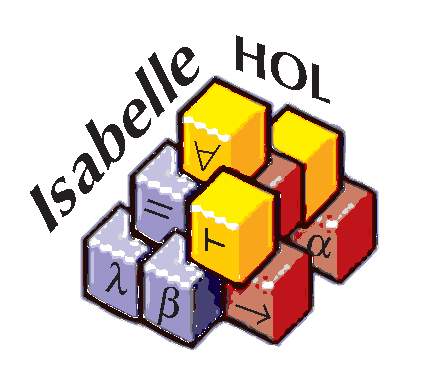
\includegraphics[scale=.8]{isabelle_hol}
       \\ \vspace{0.5cm} A Proof Assistant for Higher-Order Logic
\end{center}}
\author{Tobias Nipkow \quad Lawrence C. Paulson \quad Markus Wenzel%\\[1ex]
%Technische Universit{\"a}t M{\"u}nchen \\
%Institut f{\"u}r Informatik \\[1ex]
%University of Cambridge\\
%Computer Laboratory
}
\pagenumbering{roman}
\maketitle
\newpage

%\setcounter{page}{5}
%\vspace*{\fill}
%\begin{center}
%\LARGE In memoriam \\[1ex]
%{\sc Annette Schumann}\\[1ex]
%1959 -- 2001
%\end{center}
%\vspace*{\fill}
%\vspace*{\fill}
%\newpage

\chapter*{Preface}
\markboth{Preface}{Preface}

This volume is a self-contained introduction to interactive proof
in higher-order logic (HOL), using the proof assistant Isabelle/HOL\@. 
Compared with existing Isabelle documentation,
it provides a direct route into higher-order logic, which most people
prefer these days. It bypasses first-order logic and minimizes
discussion of meta-theory.  It is written for potential users rather
than for our colleagues in the research world.

\index{Wenzel, Markus}%
Another departure from previous documentation is that we describe Markus
Wenzel's proof script notation instead of ML tactic scripts.  The latter
make it easier to introduce new tactics on the fly, but hardly anybody
does that.  Wenzel's dedicated syntax is elegant, replacing for example
eight simplification tactics with a single method, namely \isa{simp},
with associated options.

The book has three parts.  
\begin{itemize}
\item 
The first part, \textbf{Basic Techniques},
shows how to model functional programs in higher-order logic.  Early
examples involve lists and the natural numbers.  Most proofs
are two steps long, consisting of induction on a chosen variable
followed by the \isa{auto} tactic.  But even this elementary part
covers such advanced topics as nested and mutual recursion.
\item 
The second part, \textbf{Logic and Sets}, presents a collection of
lower-level tactics that you can use to apply rules selectively.  It
also describes Isabelle/HOL's treatment of sets, functions and
relations and explains how to define sets inductively.  One of the
examples concerns the theory of model checking, and another is drawn
from a classic textbook on formal languages.
\item 
The third part, \textbf{Advanced Material}, describes a variety of
other topics.  Among these are the real numbers, records and
overloading.  Esoteric techniques are described involving induction and
recursion.  A whole chapter is devoted to an extended example: the
verification of a security protocol.
\end{itemize}

The typesetting relies on Wenzel's theory presentation tools.  An
annotated source file is run, typesetting the theory
% and any requested Isabelle responses
in the form of a \LaTeX\ source file.  This book is derived almost entirely
from output generated in this way.  The final chapter of Part~I explains how
users may produce their own formal documents in a similar fashion.

Isabelle's \hfootref{http://isabelle.in.tum.de/}{web site} contains links to
the download area and to documentation and other information.  Most Isabelle
sessions are now run from within David Aspinall's\index{Aspinall, David}
wonderful user interface, \hfootref{http://www.proofgeneral.org/}{Proof
  General}, even together with the
\hfootref{http://www.fmi.uni-passau.de/~wedler/x-symbol/}{X-Symbol} package
for XEmacs.  This book says very little about Proof General, which has its own
documentation.  In order to run Isabelle, you will need a Standard ML
compiler.  We recommend \hfootref{http://www.polyml.org/}{Poly/ML}, which is
free and gives the best performance.  The other fully supported compiler is
\hfootref{http://cm.bell-labs.com/cm/cs/what/smlnj/index.html}{Standard ML of
  New Jersey}.

This tutorial owes a lot to the constant discussions with and the valuable
feedback from the Isabelle group at Munich: Stefan Berghofer, Olaf
M{\"u}ller, Wolfgang Naraschewski, David von Oheimb, Leonor Prensa Nieto,
Cornelia Pusch, Norbert Schirmer, Martin Strecker and Markus Wenzel. Stephan
Merz was also kind enough to read and comment on a draft version.  We
received comments from Stefano Bistarelli, Gergely Buday and Tanja
Vos.

The research has been funded by many sources, including the {\sc dfg} grants
Ni~491/2, Ni~491/3, Ni~491/4 and the {\sc epsrc} grants GR\slash K57381,
GR\slash K77051, GR\slash M75440, GR\slash R01156\slash 01 and by the
\textsc{esprit} working groups 21900 and IST-1999-29001 (the \emph{Types}
project).


\tableofcontents

\cleardoublepage\pagenumbering{arabic}

\part{Elementary Techniques}
\chapter{The Basics}

\section{Introduction}

This book is a tutorial on how to use the theorem prover Isabelle/HOL as a
specification and verification system. Isabelle is a generic system for
implementing logical formalisms, and Isabelle/HOL is the specialization
of Isabelle for HOL, which abbreviates Higher-Order Logic. We introduce
HOL step by step following the equation
\[ \mbox{HOL} = \mbox{Functional Programming} + \mbox{Logic}. \]
We do not assume that you are familiar with mathematical logic. 
However, we do assume that
you are used to logical and set theoretic notation, as covered
in a good discrete mathematics course~\cite{Rosen-DMA}, and
that you are familiar with the basic concepts of functional
programming~\cite{Bird-Haskell,Hudak-Haskell,paulson-ml2,Thompson-Haskell}.
Although this tutorial initially concentrates on functional programming, do
not be misled: HOL can express most mathematical concepts, and functional
programming is just one particularly simple and ubiquitous instance.

Isabelle~\cite{paulson-isa-book} is implemented in ML~\cite{SML}.  This has
influenced some of Isabelle/HOL's concrete syntax but is otherwise irrelevant
for us: this tutorial is based on
Isabelle/Isar~\cite{isabelle-isar-ref}, an extension of Isabelle which hides
the implementation language almost completely.  Thus the full name of the
system should be Isabelle/Isar/HOL, but that is a bit of a mouthful.

There are other implementations of HOL, in particular the one by Mike Gordon
\index{Gordon, Mike}%
\emph{et al.}, which is usually referred to as ``the HOL system''
\cite{mgordon-hol}. For us, HOL refers to the logical system, and sometimes
its incarnation Isabelle/HOL\@.

A tutorial is by definition incomplete.  Currently the tutorial only
introduces the rudiments of Isar's proof language. To fully exploit the power
of Isar, in particular the ability to write readable and structured proofs,
you need to consult the Isabelle/Isar Reference
Manual~\cite{isabelle-isar-ref} and Wenzel's PhD thesis~\cite{Wenzel-PhD}
which discusses many proof patterns. If you want to use Isabelle's ML level
directly (for example for writing your own proof procedures) see the Isabelle
Reference Manual~\cite{isabelle-ref}; for details relating to HOL see the
Isabelle/HOL manual~\cite{isabelle-HOL}. All manuals have a comprehensive
index.

\section{Theories}
\label{sec:Basic:Theories}

\index{theories|(}%
Working with Isabelle means creating theories. Roughly speaking, a
\textbf{theory} is a named collection of types, functions, and theorems,
much like a module in a programming language or a specification in a
specification language. In fact, theories in HOL can be either. The general
format of a theory \texttt{T} is
\begin{ttbox}
theory T
imports B\(@1\) \(\ldots\) B\(@n\)
begin
{\rmfamily\textit{declarations, definitions, and proofs}}
end
\end{ttbox}\cmmdx{theory}\cmmdx{imports}
where \texttt{B}$@1$ \dots\ \texttt{B}$@n$ are the names of existing
theories that \texttt{T} is based on and \textit{declarations,
    definitions, and proofs} represents the newly introduced concepts
(types, functions etc.) and proofs about them. The \texttt{B}$@i$ are the
direct \textbf{parent theories}\indexbold{parent theories} of~\texttt{T}\@.
Everything defined in the parent theories (and their parents, recursively) is
automatically visible. To avoid name clashes, identifiers can be
\textbf{qualified}\indexbold{identifiers!qualified}
by theory names as in \texttt{T.f} and~\texttt{B.f}. 
Each theory \texttt{T} must
reside in a \textbf{theory file}\index{theory files} named \texttt{T.thy}.

This tutorial is concerned with introducing you to the different linguistic
constructs that can fill the \textit{declarations, definitions, and
    proofs} above.  A complete grammar of the basic
constructs is found in the Isabelle/Isar Reference
Manual~\cite{isabelle-isar-ref}.

HOL's theory collection is available online at
\begin{center}\small
    \url{http://isabelle.in.tum.de/library/HOL/}
\end{center}
and is recommended browsing. Note that most of the theories 
are based on classical Isabelle without the Isar extension. This means that
they look slightly different than the theories in this tutorial, and that all
proofs are in separate ML files.

\begin{warn}
  HOL contains a theory \thydx{Main}, the union of all the basic
  predefined theories like arithmetic, lists, sets, etc.  
  Unless you know what you are doing, always include \isa{Main}
  as a direct or indirect parent of all your theories.
\end{warn}
There is also a growing Library~\cite{HOL-Library}\index{Library}
of useful theories that are not part of \isa{Main} but can be included
among the parents of a theory and will then be loaded automatically.%
\index{theories|)}


\section{Types, Terms and Formulae}
\label{sec:TypesTermsForms}

Embedded in a theory are the types, terms and formulae of HOL\@. HOL is a typed
logic whose type system resembles that of functional programming languages
like ML or Haskell. Thus there are
\index{types|(}
\begin{description}
\item[base types,] 
in particular \tydx{bool}, the type of truth values,
and \tydx{nat}, the type of natural numbers.
\item[type constructors,]\index{type constructors}
 in particular \tydx{list}, the type of
lists, and \tydx{set}, the type of sets. Type constructors are written
postfix, e.g.\ \isa{(nat)list} is the type of lists whose elements are
natural numbers. Parentheses around single arguments can be dropped (as in
\isa{nat list}), multiple arguments are separated by commas (as in
\isa{(bool,nat)ty}).
\item[function types,]\index{function types}
denoted by \isasymFun\indexbold{$IsaFun@\isasymFun}.
  In HOL \isasymFun\ represents \emph{total} functions only. As is customary,
  \isa{$\tau@1$ \isasymFun~$\tau@2$ \isasymFun~$\tau@3$} means
  \isa{$\tau@1$ \isasymFun~($\tau@2$ \isasymFun~$\tau@3$)}. Isabelle also
  supports the notation \isa{[$\tau@1,\dots,\tau@n$] \isasymFun~$\tau$}
  which abbreviates \isa{$\tau@1$ \isasymFun~$\cdots$ \isasymFun~$\tau@n$
    \isasymFun~$\tau$}.
\item[type variables,]\index{type variables}\index{variables!type}
  denoted by \ttindexboldpos{'a}{$Isatype}, \isa{'b} etc., just like in ML\@. They give rise
  to polymorphic types like \isa{'a \isasymFun~'a}, the type of the identity
  function.
\end{description}
\begin{warn}
  Types are extremely important because they prevent us from writing
  nonsense.  Isabelle insists that all terms and formulae must be well-typed
  and will print an error message if a type mismatch is encountered. To
  reduce the amount of explicit type information that needs to be provided by
  the user, Isabelle infers the type of all variables automatically (this is
  called \bfindex{type inference}) and keeps quiet about it. Occasionally
  this may lead to misunderstandings between you and the system. If anything
  strange happens, we recommend that you set the flag\index{flags}
  \isa{show_types}\index{*show_types (flag)}.  
  Isabelle will then display type information
  that is usually suppressed.  Simply type
\begin{ttbox}
ML "set show_types"
\end{ttbox}

\noindent
This can be reversed by \texttt{ML "reset show_types"}. Various other flags,
which we introduce as we go along, can be set and reset in the same manner.%
\index{flags!setting and resetting}
\end{warn}%
\index{types|)}


\index{terms|(}
\textbf{Terms} are formed as in functional programming by
applying functions to arguments. If \isa{f} is a function of type
\isa{$\tau@1$ \isasymFun~$\tau@2$} and \isa{t} is a term of type
$\tau@1$ then \isa{f~t} is a term of type $\tau@2$. HOL also supports
infix functions like \isa{+} and some basic constructs from functional
programming, such as conditional expressions:
\begin{description}
\item[\isa{if $b$ then $t@1$ else $t@2$}]\index{*if expressions}
Here $b$ is of type \isa{bool} and $t@1$ and $t@2$ are of the same type.
\item[\isa{let $x$ = $t$ in $u$}]\index{*let expressions}
is equivalent to $u$ where all free occurrences of $x$ have been replaced by
$t$. For example,
\isa{let x = 0 in x+x} is equivalent to \isa{0+0}. Multiple bindings are separated
by semicolons: \isa{let $x@1$ = $t@1$;\dots; $x@n$ = $t@n$ in $u$}.
\item[\isa{case $e$ of $c@1$ \isasymFun~$e@1$ |~\dots~| $c@n$ \isasymFun~$e@n$}]
\index{*case expressions}
evaluates to $e@i$ if $e$ is of the form $c@i$.
\end{description}

Terms may also contain
\isasymlambda-abstractions.\index{lambda@$\lambda$ expressions}
For example,
\isa{\isasymlambda{}x.~x+1} is the function that takes an argument \isa{x} and
returns \isa{x+1}. Instead of
\isa{\isasymlambda{}x.\isasymlambda{}y.\isasymlambda{}z.~$t$} we can write
\isa{\isasymlambda{}x~y~z.~$t$}.%
\index{terms|)}

\index{formulae|(}%
\textbf{Formulae} are terms of type \tydx{bool}.
There are the basic constants \cdx{True} and \cdx{False} and
the usual logical connectives (in decreasing order of priority):
\indexboldpos{\protect\isasymnot}{$HOL0not}, \indexboldpos{\protect\isasymand}{$HOL0and},
\indexboldpos{\protect\isasymor}{$HOL0or}, and \indexboldpos{\protect\isasymimp}{$HOL0imp},
all of which (except the unary \isasymnot) associate to the right. In
particular \isa{A \isasymimp~B \isasymimp~C} means \isa{A \isasymimp~(B
  \isasymimp~C)} and is thus logically equivalent to \isa{A \isasymand~B
  \isasymimp~C} (which is \isa{(A \isasymand~B) \isasymimp~C}).

Equality\index{equality} is available in the form of the infix function
\isa{=} of type \isa{'a \isasymFun~'a
  \isasymFun~bool}. Thus \isa{$t@1$ = $t@2$} is a formula provided $t@1$
and $t@2$ are terms of the same type. If $t@1$ and $t@2$ are of type
\isa{bool} then \isa{=} acts as \rmindex{if-and-only-if}.
The formula
\isa{$t@1$~\isasymnoteq~$t@2$} is merely an abbreviation for
\isa{\isasymnot($t@1$ = $t@2$)}.

Quantifiers\index{quantifiers} are written as
\isa{\isasymforall{}x.~$P$} and \isa{\isasymexists{}x.~$P$}. 
There is even
\isa{\isasymuniqex{}x.~$P$}, which
means that there exists exactly one \isa{x} that satisfies \isa{$P$}. 
Nested quantifications can be abbreviated:
\isa{\isasymforall{}x~y~z.~$P$} means
\isa{\isasymforall{}x.\isasymforall{}y.\isasymforall{}z.~$P$}.%
\index{formulae|)}

Despite type inference, it is sometimes necessary to attach explicit
\bfindex{type constraints} to a term.  The syntax is
\isa{$t$::$\tau$} as in \isa{x < (y::nat)}. Note that
\ttindexboldpos{::}{$Isatype} binds weakly and should therefore be enclosed
in parentheses.  For instance,
\isa{x < y::nat} is ill-typed because it is interpreted as
\isa{(x < y)::nat}.  Type constraints may be needed to disambiguate
expressions
involving overloaded functions such as~\isa{+}, 
\isa{*} and~\isa{<}.  Section~\ref{sec:overloading} 
discusses overloading, while Table~\ref{tab:overloading} presents the most
important overloaded function symbols.

In general, HOL's concrete \rmindex{syntax} tries to follow the conventions of
functional programming and mathematics.  Here are the main rules that you
should be familiar with to avoid certain syntactic traps:
\begin{itemize}
\item
Remember that \isa{f t u} means \isa{(f t) u} and not \isa{f(t u)}!
\item
Isabelle allows infix functions like \isa{+}. The prefix form of function
application binds more strongly than anything else and hence \isa{f~x + y}
means \isa{(f~x)~+~y} and not \isa{f(x+y)}.
\item Remember that in HOL if-and-only-if is expressed using equality.  But
  equality has a high priority, as befitting a relation, while if-and-only-if
  typically has the lowest priority.  Thus, \isa{\isasymnot~\isasymnot~P =
    P} means \isa{\isasymnot\isasymnot(P = P)} and not
  \isa{(\isasymnot\isasymnot P) = P}. When using \isa{=} to mean
  logical equivalence, enclose both operands in parentheses, as in \isa{(A
    \isasymand~B) = (B \isasymand~A)}.
\item
Constructs with an opening but without a closing delimiter bind very weakly
and should therefore be enclosed in parentheses if they appear in subterms, as
in \isa{(\isasymlambda{}x.~x) = f}.  This includes 
\isa{if},\index{*if expressions}
\isa{let},\index{*let expressions}
\isa{case},\index{*case expressions}
\isa{\isasymlambda}, and quantifiers.
\item
Never write \isa{\isasymlambda{}x.x} or \isa{\isasymforall{}x.x=x}
because \isa{x.x} is always taken as a single qualified identifier. Write
\isa{\isasymlambda{}x.~x} and \isa{\isasymforall{}x.~x=x} instead.
\item Identifiers\indexbold{identifiers} may contain the characters \isa{_} 
and~\isa{'}, except at the beginning.
\end{itemize}

For the sake of readability, we use the usual mathematical symbols throughout
the tutorial. Their \textsc{ascii}-equivalents are shown in table~\ref{tab:ascii} in
the appendix.

\begin{warn}
A particular
problem for novices can be the priority of operators. If you are unsure, use
additional parentheses. In those cases where Isabelle echoes your
input, you can see which parentheses are dropped --- they were superfluous. If
you are unsure how to interpret Isabelle's output because you don't know
where the (dropped) parentheses go, set the flag\index{flags}
\isa{show_brackets}\index{*show_brackets (flag)}:
\begin{ttbox}
ML "set show_brackets"; \(\dots\); ML "reset show_brackets";
\end{ttbox}
\end{warn}


\section{Variables}
\label{sec:variables}
\index{variables|(}

Isabelle distinguishes free and bound variables, as is customary. Bound
variables are automatically renamed to avoid clashes with free variables. In
addition, Isabelle has a third kind of variable, called a \textbf{schematic
  variable}\index{variables!schematic} or \textbf{unknown}\index{unknowns}, 
which must have a~\isa{?} as its first character.  
Logically, an unknown is a free variable. But it may be
instantiated by another term during the proof process. For example, the
mathematical theorem $x = x$ is represented in Isabelle as \isa{?x = ?x},
which means that Isabelle can instantiate it arbitrarily. This is in contrast
to ordinary variables, which remain fixed. The programming language Prolog
calls unknowns {\em logical\/} variables.

Most of the time you can and should ignore unknowns and work with ordinary
variables. Just don't be surprised that after you have finished the proof of
a theorem, Isabelle will turn your free variables into unknowns.  It
indicates that Isabelle will automatically instantiate those unknowns
suitably when the theorem is used in some other proof.
Note that for readability we often drop the \isa{?}s when displaying a theorem.
\begin{warn}
  For historical reasons, Isabelle accepts \isa{?} as an ASCII representation
  of the \(\exists\) symbol.  However, the \isa{?} character must then be followed
  by a space, as in \isa{?~x. f(x) = 0}.  Otherwise, \isa{?x} is
  interpreted as a schematic variable.  The preferred ASCII representation of
  the \(\exists\) symbol is \isa{EX}\@. 
\end{warn}%
\index{variables|)}

\section{Interaction and Interfaces}

Interaction with Isabelle can either occur at the shell level or through more
advanced interfaces. To keep the tutorial independent of the interface, we
have phrased the description of the interaction in a neutral language. For
example, the phrase ``to abandon a proof'' means to type \isacommand{oops} at the
shell level, which is explained the first time the phrase is used. Other
interfaces perform the same act by cursor movements and/or mouse clicks.
Although shell-based interaction is quite feasible for the kind of proof
scripts currently presented in this tutorial, the recommended interface for
Isabelle/Isar is the Emacs-based \bfindex{Proof
  General}~\cite{proofgeneral,Aspinall:TACAS:2000}.

Some interfaces (including the shell level) offer special fonts with
mathematical symbols. For those that do not, remember that \textsc{ascii}-equivalents
are shown in table~\ref{tab:ascii} in the appendix.

Finally, a word about semicolons.\indexbold{$Isar@\texttt{;}} 
Commands may but need not be terminated by semicolons.
At the shell level it is advisable to use semicolons to enforce that a command
is executed immediately; otherwise Isabelle may wait for the next keyword
before it knows that the command is complete.


\section{Getting Started}

Assuming you have installed Isabelle, you start it by typing \texttt{isabelle
  -I HOL} in a shell window.\footnote{Simply executing \texttt{isabelle -I}
  starts the default logic, which usually is already \texttt{HOL}.  This is
  controlled by the \texttt{ISABELLE_LOGIC} setting, see \emph{The Isabelle
    System Manual} for more details.} This presents you with Isabelle's most
basic \textsc{ascii} interface.  In addition you need to open an editor window to
create theory files.  While you are developing a theory, we recommend that you
type each command into the file first and then enter it into Isabelle by
copy-and-paste, thus ensuring that you have a complete record of your theory.
As mentioned above, Proof General offers a much superior interface.
If you have installed Proof General, you can start it by typing \texttt{Isabelle}.

\chapter{Functional Programming in HOL}

This chapter describes how to write
functional programs in HOL and how to verify them.  However, 
most of the constructs and
proof procedures introduced are general and recur in any specification
or verification task.  We really should speak of functional
\emph{modelling} rather than functional \emph{programming}: 
our primary aim is not
to write programs but to design abstract models of systems.  HOL is
a specification language that goes well beyond what can be expressed as a
program. However, for the time being we concentrate on the computable.

If you are a purist functional programmer, please note that all functions
in HOL must be total:
they must terminate for all inputs.  Lazy data structures are not
directly available.

\section{An Introductory Theory}
\label{sec:intro-theory}

Functional programming needs datatypes and functions. Both of them can be
defined in a theory with a syntax reminiscent of languages like ML or
Haskell. As an example consider the theory in figure~\ref{fig:ToyList}.
We will now examine it line by line.

\begin{figure}[htbp]
\begin{ttbox}\makeatother
\input{ToyList2/ToyList1}\end{ttbox}
\caption{A Theory of Lists}
\label{fig:ToyList}
\end{figure}

\index{*ToyList example|(}
{\makeatother%
\begin{isabellebody}%
\def\isabellecontext{ToyList}%
%
\isadelimtheory
%
\endisadelimtheory
%
\isatagtheory
\isacommand{theory}\isamarkupfalse%
\ ToyList\isanewline
\isakeyword{imports}\ PreList\isanewline
\isakeyword{begin}%
\endisatagtheory
{\isafoldtheory}%
%
\isadelimtheory
%
\endisadelimtheory
%
\begin{isamarkuptext}%
\noindent
HOL already has a predefined theory of lists called \isa{List} ---
\isa{ToyList} is merely a small fragment of it chosen as an example. In
contrast to what is recommended in \S\ref{sec:Basic:Theories},
\isa{ToyList} is not based on \isa{Main} but on \isa{PreList}, a
theory that contains pretty much everything but lists, thus avoiding
ambiguities caused by defining lists twice.%
\end{isamarkuptext}%
\isamarkuptrue%
\isacommand{datatype}\isamarkupfalse%
\ {\isacharprime}a\ list\ {\isacharequal}\ Nil\ \ \ \ \ \ \ \ \ \ \ \ \ \ \ \ \ \ \ \ \ \ \ \ \ \ {\isacharparenleft}{\isachardoublequoteopen}{\isacharbrackleft}{\isacharbrackright}{\isachardoublequoteclose}{\isacharparenright}\isanewline
\ \ \ \ \ \ \ \ \ \ \ \ \ \ \ \ \ {\isacharbar}\ Cons\ {\isacharprime}a\ {\isachardoublequoteopen}{\isacharprime}a\ list{\isachardoublequoteclose}\ \ \ \ \ \ \ \ \ \ \ \ {\isacharparenleft}\isakeyword{infixr}\ {\isachardoublequoteopen}{\isacharhash}{\isachardoublequoteclose}\ {\isadigit{6}}{\isadigit{5}}{\isacharparenright}%
\begin{isamarkuptext}%
\noindent
The datatype\index{datatype@\isacommand {datatype} (command)}
\tydx{list} introduces two
constructors \cdx{Nil} and \cdx{Cons}, the
empty~list and the operator that adds an element to the front of a list. For
example, the term \isa{Cons True (Cons False Nil)} is a value of
type \isa{bool\ list}, namely the list with the elements \isa{True} and
\isa{False}. Because this notation quickly becomes unwieldy, the
datatype declaration is annotated with an alternative syntax: instead of
\isa{Nil} and \isa{Cons x xs} we can write
\isa{{\isacharbrackleft}{\isacharbrackright}}\index{$HOL2list@\isa{[]}|bold} and
\isa{x\ {\isacharhash}\ xs}\index{$HOL2list@\isa{\#}|bold}. In fact, this
alternative syntax is the familiar one.  Thus the list \isa{Cons True
(Cons False Nil)} becomes \isa{True\ {\isacharhash}\ False\ {\isacharhash}\ {\isacharbrackleft}{\isacharbrackright}}. The annotation
\isacommand{infixr}\index{infixr@\isacommand{infixr} (annotation)} 
means that \isa{{\isacharhash}} associates to
the right: the term \isa{x\ {\isacharhash}\ y\ {\isacharhash}\ z} is read as \isa{x\ {\isacharhash}\ {\isacharparenleft}y\ {\isacharhash}\ z{\isacharparenright}}
and not as \isa{{\isacharparenleft}x\ {\isacharhash}\ y{\isacharparenright}\ {\isacharhash}\ z}.
The \isa{{\isadigit{6}}{\isadigit{5}}} is the priority of the infix \isa{{\isacharhash}}.

\begin{warn}
  Syntax annotations can be powerful, but they are difficult to master and 
  are never necessary.  You
  could drop them from theory \isa{ToyList} and go back to the identifiers
  \isa{Nil} and \isa{Cons}.
  Novices should avoid using
  syntax annotations in their own theories.
\end{warn}
Next, two functions \isa{app} and \cdx{rev} are declared:%
\end{isamarkuptext}%
\isamarkuptrue%
\isacommand{consts}\isamarkupfalse%
\ app\ {\isacharcolon}{\isacharcolon}\ {\isachardoublequoteopen}{\isacharprime}a\ list\ {\isasymRightarrow}\ {\isacharprime}a\ list\ {\isasymRightarrow}\ {\isacharprime}a\ list{\isachardoublequoteclose}\ \ \ {\isacharparenleft}\isakeyword{infixr}\ {\isachardoublequoteopen}{\isacharat}{\isachardoublequoteclose}\ {\isadigit{6}}{\isadigit{5}}{\isacharparenright}\isanewline
\ \ \ \ \ \ \ rev\ {\isacharcolon}{\isacharcolon}\ {\isachardoublequoteopen}{\isacharprime}a\ list\ {\isasymRightarrow}\ {\isacharprime}a\ list{\isachardoublequoteclose}%
\begin{isamarkuptext}%
\noindent
In contrast to many functional programming languages,
Isabelle insists on explicit declarations of all functions
(keyword \commdx{consts}).  Apart from the declaration-before-use
restriction, the order of items in a theory file is unconstrained. Function
\isa{app} is annotated with concrete syntax too. Instead of the
prefix syntax \isa{app\ xs\ ys} the infix
\isa{xs\ {\isacharat}\ ys}\index{$HOL2list@\isa{\at}|bold} becomes the preferred
form. Both functions are defined recursively:%
\end{isamarkuptext}%
\isamarkuptrue%
\isacommand{primrec}\isamarkupfalse%
\isanewline
{\isachardoublequoteopen}{\isacharbrackleft}{\isacharbrackright}\ {\isacharat}\ ys\ \ \ \ \ \ \ {\isacharequal}\ ys{\isachardoublequoteclose}\isanewline
{\isachardoublequoteopen}{\isacharparenleft}x\ {\isacharhash}\ xs{\isacharparenright}\ {\isacharat}\ ys\ {\isacharequal}\ x\ {\isacharhash}\ {\isacharparenleft}xs\ {\isacharat}\ ys{\isacharparenright}{\isachardoublequoteclose}\isanewline
\isanewline
\isacommand{primrec}\isamarkupfalse%
\isanewline
{\isachardoublequoteopen}rev\ {\isacharbrackleft}{\isacharbrackright}\ \ \ \ \ \ \ \ {\isacharequal}\ {\isacharbrackleft}{\isacharbrackright}{\isachardoublequoteclose}\isanewline
{\isachardoublequoteopen}rev\ {\isacharparenleft}x\ {\isacharhash}\ xs{\isacharparenright}\ \ {\isacharequal}\ {\isacharparenleft}rev\ xs{\isacharparenright}\ {\isacharat}\ {\isacharparenleft}x\ {\isacharhash}\ {\isacharbrackleft}{\isacharbrackright}{\isacharparenright}{\isachardoublequoteclose}%
\begin{isamarkuptext}%
\noindent\index{*rev (constant)|(}\index{append function|(}
The equations for \isa{app} and \isa{rev} hardly need comments:
\isa{app} appends two lists and \isa{rev} reverses a list.  The
keyword \commdx{primrec} indicates that the recursion is
of a particularly primitive kind where each recursive call peels off a datatype
constructor from one of the arguments.  Thus the
recursion always terminates, i.e.\ the function is \textbf{total}.
\index{functions!total}

The termination requirement is absolutely essential in HOL, a logic of total
functions. If we were to drop it, inconsistencies would quickly arise: the
``definition'' $f(n) = f(n)+1$ immediately leads to $0 = 1$ by subtracting
$f(n)$ on both sides.
% However, this is a subtle issue that we cannot discuss here further.

\begin{warn}
  As we have indicated, the requirement for total functions is an essential characteristic of HOL\@. It is only
  because of totality that reasoning in HOL is comparatively easy.  More
  generally, the philosophy in HOL is to refrain from asserting arbitrary axioms (such as
  function definitions whose totality has not been proved) because they
  quickly lead to inconsistencies. Instead, fixed constructs for introducing
  types and functions are offered (such as \isacommand{datatype} and
  \isacommand{primrec}) which are guaranteed to preserve consistency.
\end{warn}

\index{syntax}%
A remark about syntax.  The textual definition of a theory follows a fixed
syntax with keywords like \isacommand{datatype} and \isacommand{end}.
% (see Fig.~\ref{fig:keywords} in Appendix~\ref{sec:Appendix} for a full list).
Embedded in this syntax are the types and formulae of HOL, whose syntax is
extensible (see \S\ref{sec:concrete-syntax}), e.g.\ by new user-defined infix operators.
To distinguish the two levels, everything
HOL-specific (terms and types) should be enclosed in
\texttt{"}\dots\texttt{"}. 
To lessen this burden, quotation marks around a single identifier can be
dropped, unless the identifier happens to be a keyword, as in%
\end{isamarkuptext}%
\isamarkuptrue%
\isacommand{consts}\isamarkupfalse%
\ {\isachardoublequoteopen}end{\isachardoublequoteclose}\ {\isacharcolon}{\isacharcolon}\ {\isachardoublequoteopen}{\isacharprime}a\ list\ {\isasymRightarrow}\ {\isacharprime}a{\isachardoublequoteclose}%
\begin{isamarkuptext}%
\noindent
When Isabelle prints a syntax error message, it refers to the HOL syntax as
the \textbf{inner syntax} and the enclosing theory language as the \textbf{outer syntax}.


\section{An Introductory Proof}
\label{sec:intro-proof}

Assuming you have processed the declarations and definitions of
\texttt{ToyList} presented so far, we are ready to prove a few simple
theorems. This will illustrate not just the basic proof commands but
also the typical proof process.

\subsubsection*{Main Goal.}

Our goal is to show that reversing a list twice produces the original
list.%
\end{isamarkuptext}%
\isamarkuptrue%
\isacommand{theorem}\isamarkupfalse%
\ rev{\isacharunderscore}rev\ {\isacharbrackleft}simp{\isacharbrackright}{\isacharcolon}\ {\isachardoublequoteopen}rev{\isacharparenleft}rev\ xs{\isacharparenright}\ {\isacharequal}\ xs{\isachardoublequoteclose}%
\isadelimproof
%
\endisadelimproof
%
\isatagproof
%
\begin{isamarkuptxt}%
\index{theorem@\isacommand {theorem} (command)|bold}%
\noindent
This \isacommand{theorem} command does several things:
\begin{itemize}
\item
It establishes a new theorem to be proved, namely \isa{rev\ {\isacharparenleft}rev\ xs{\isacharparenright}\ {\isacharequal}\ xs}.
\item
It gives that theorem the name \isa{rev{\isacharunderscore}rev}, for later reference.
\item
It tells Isabelle (via the bracketed attribute \attrdx{simp}) to take the eventual theorem as a simplification rule: future proofs involving
simplification will replace occurrences of \isa{rev\ {\isacharparenleft}rev\ xs{\isacharparenright}} by
\isa{xs}.
\end{itemize}
The name and the simplification attribute are optional.
Isabelle's response is to print the initial proof state consisting
of some header information (like how many subgoals there are) followed by
\begin{isabelle}%
\ {\isadigit{1}}{\isachardot}\ rev\ {\isacharparenleft}rev\ xs{\isacharparenright}\ {\isacharequal}\ xs%
\end{isabelle}
For compactness reasons we omit the header in this tutorial.
Until we have finished a proof, the \rmindex{proof state} proper
always looks like this:
\begin{isabelle}
~1.~$G\sb{1}$\isanewline
~~\vdots~~\isanewline
~$n$.~$G\sb{n}$
\end{isabelle}
The numbered lines contain the subgoals $G\sb{1}$, \dots, $G\sb{n}$
that we need to prove to establish the main goal.\index{subgoals}
Initially there is only one subgoal, which is identical with the
main goal. (If you always want to see the main goal as well,
set the flag \isa{Proof.show_main_goal}\index{*show_main_goal (flag)}
--- this flag used to be set by default.)

Let us now get back to \isa{rev\ {\isacharparenleft}rev\ xs{\isacharparenright}\ {\isacharequal}\ xs}. Properties of recursively
defined functions are best established by induction. In this case there is
nothing obvious except induction on \isa{xs}:%
\end{isamarkuptxt}%
\isamarkuptrue%
\isacommand{apply}\isamarkupfalse%
{\isacharparenleft}induct{\isacharunderscore}tac\ xs{\isacharparenright}%
\begin{isamarkuptxt}%
\noindent\index{*induct_tac (method)}%
This tells Isabelle to perform induction on variable \isa{xs}. The suffix
\isa{tac} stands for \textbf{tactic},\index{tactics}
a synonym for ``theorem proving function''.
By default, induction acts on the first subgoal. The new proof state contains
two subgoals, namely the base case (\isa{Nil}) and the induction step
(\isa{Cons}):
\begin{isabelle}%
\ {\isadigit{1}}{\isachardot}\ rev\ {\isacharparenleft}rev\ {\isacharbrackleft}{\isacharbrackright}{\isacharparenright}\ {\isacharequal}\ {\isacharbrackleft}{\isacharbrackright}\isanewline
\ {\isadigit{2}}{\isachardot}\ {\isasymAnd}a\ list{\isachardot}\isanewline
\isaindent{\ {\isadigit{2}}{\isachardot}\ \ \ \ }rev\ {\isacharparenleft}rev\ list{\isacharparenright}\ {\isacharequal}\ list\ {\isasymLongrightarrow}\ rev\ {\isacharparenleft}rev\ {\isacharparenleft}a\ {\isacharhash}\ list{\isacharparenright}{\isacharparenright}\ {\isacharequal}\ a\ {\isacharhash}\ list%
\end{isabelle}

The induction step is an example of the general format of a subgoal:\index{subgoals}
\begin{isabelle}
~$i$.~{\isasymAnd}$x\sb{1}$~\dots$x\sb{n}$.~{\it assumptions}~{\isasymLongrightarrow}~{\it conclusion}
\end{isabelle}\index{$IsaAnd@\isasymAnd|bold}
The prefix of bound variables \isasymAnd$x\sb{1}$~\dots~$x\sb{n}$ can be
ignored most of the time, or simply treated as a list of variables local to
this subgoal. Their deeper significance is explained in Chapter~\ref{chap:rules}.
The {\it assumptions}\index{assumptions!of subgoal}
are the local assumptions for this subgoal and {\it
  conclusion}\index{conclusion!of subgoal} is the actual proposition to be proved. 
Typical proof steps
that add new assumptions are induction and case distinction. In our example
the only assumption is the induction hypothesis \isa{rev\ {\isacharparenleft}rev\ list{\isacharparenright}\ {\isacharequal}\ list}, where \isa{list} is a variable name chosen by Isabelle. If there
are multiple assumptions, they are enclosed in the bracket pair
\indexboldpos{\isasymlbrakk}{$Isabrl} and
\indexboldpos{\isasymrbrakk}{$Isabrr} and separated by semicolons.

Let us try to solve both goals automatically:%
\end{isamarkuptxt}%
\isamarkuptrue%
\isacommand{apply}\isamarkupfalse%
{\isacharparenleft}auto{\isacharparenright}%
\begin{isamarkuptxt}%
\noindent
This command tells Isabelle to apply a proof strategy called
\isa{auto} to all subgoals. Essentially, \isa{auto} tries to
simplify the subgoals.  In our case, subgoal~1 is solved completely (thanks
to the equation \isa{rev\ {\isacharbrackleft}{\isacharbrackright}\ {\isacharequal}\ {\isacharbrackleft}{\isacharbrackright}}) and disappears; the simplified version
of subgoal~2 becomes the new subgoal~1:
\begin{isabelle}%
\ {\isadigit{1}}{\isachardot}\ {\isasymAnd}a\ list{\isachardot}\isanewline
\isaindent{\ {\isadigit{1}}{\isachardot}\ \ \ \ }rev\ {\isacharparenleft}rev\ list{\isacharparenright}\ {\isacharequal}\ list\ {\isasymLongrightarrow}\ rev\ {\isacharparenleft}rev\ list\ {\isacharat}\ a\ {\isacharhash}\ {\isacharbrackleft}{\isacharbrackright}{\isacharparenright}\ {\isacharequal}\ a\ {\isacharhash}\ list%
\end{isabelle}
In order to simplify this subgoal further, a lemma suggests itself.%
\end{isamarkuptxt}%
\isamarkuptrue%
%
\endisatagproof
{\isafoldproof}%
%
\isadelimproof
%
\endisadelimproof
%
\isamarkupsubsubsection{First Lemma%
}
\isamarkuptrue%
%
\begin{isamarkuptext}%
\indexbold{abandoning a proof}\indexbold{proofs!abandoning}
After abandoning the above proof attempt (at the shell level type
\commdx{oops}) we start a new proof:%
\end{isamarkuptext}%
\isamarkuptrue%
\isacommand{lemma}\isamarkupfalse%
\ rev{\isacharunderscore}app\ {\isacharbrackleft}simp{\isacharbrackright}{\isacharcolon}\ {\isachardoublequoteopen}rev{\isacharparenleft}xs\ {\isacharat}\ ys{\isacharparenright}\ {\isacharequal}\ {\isacharparenleft}rev\ ys{\isacharparenright}\ {\isacharat}\ {\isacharparenleft}rev\ xs{\isacharparenright}{\isachardoublequoteclose}%
\isadelimproof
%
\endisadelimproof
%
\isatagproof
%
\begin{isamarkuptxt}%
\noindent The keywords \commdx{theorem} and
\commdx{lemma} are interchangeable and merely indicate
the importance we attach to a proposition.  Therefore we use the words
\emph{theorem} and \emph{lemma} pretty much interchangeably, too.

There are two variables that we could induct on: \isa{xs} and
\isa{ys}. Because \isa{{\isacharat}} is defined by recursion on
the first argument, \isa{xs} is the correct one:%
\end{isamarkuptxt}%
\isamarkuptrue%
\isacommand{apply}\isamarkupfalse%
{\isacharparenleft}induct{\isacharunderscore}tac\ xs{\isacharparenright}%
\begin{isamarkuptxt}%
\noindent
This time not even the base case is solved automatically:%
\end{isamarkuptxt}%
\isamarkuptrue%
\isacommand{apply}\isamarkupfalse%
{\isacharparenleft}auto{\isacharparenright}%
\begin{isamarkuptxt}%
\begin{isabelle}%
\ {\isadigit{1}}{\isachardot}\ rev\ ys\ {\isacharequal}\ rev\ ys\ {\isacharat}\ {\isacharbrackleft}{\isacharbrackright}%
\end{isabelle}
Again, we need to abandon this proof attempt and prove another simple lemma
first. In the future the step of abandoning an incomplete proof before
embarking on the proof of a lemma usually remains implicit.%
\end{isamarkuptxt}%
\isamarkuptrue%
%
\endisatagproof
{\isafoldproof}%
%
\isadelimproof
%
\endisadelimproof
%
\isamarkupsubsubsection{Second Lemma%
}
\isamarkuptrue%
%
\begin{isamarkuptext}%
We again try the canonical proof procedure:%
\end{isamarkuptext}%
\isamarkuptrue%
\isacommand{lemma}\isamarkupfalse%
\ app{\isacharunderscore}Nil{\isadigit{2}}\ {\isacharbrackleft}simp{\isacharbrackright}{\isacharcolon}\ {\isachardoublequoteopen}xs\ {\isacharat}\ {\isacharbrackleft}{\isacharbrackright}\ {\isacharequal}\ xs{\isachardoublequoteclose}\isanewline
%
\isadelimproof
%
\endisadelimproof
%
\isatagproof
\isacommand{apply}\isamarkupfalse%
{\isacharparenleft}induct{\isacharunderscore}tac\ xs{\isacharparenright}\isanewline
\isacommand{apply}\isamarkupfalse%
{\isacharparenleft}auto{\isacharparenright}%
\begin{isamarkuptxt}%
\noindent
It works, yielding the desired message \isa{No\ subgoals{\isacharbang}}:
\begin{isabelle}%
xs\ {\isacharat}\ {\isacharbrackleft}{\isacharbrackright}\ {\isacharequal}\ xs\isanewline
No\ subgoals{\isacharbang}%
\end{isabelle}
We still need to confirm that the proof is now finished:%
\end{isamarkuptxt}%
\isamarkuptrue%
\isacommand{done}\isamarkupfalse%
%
\endisatagproof
{\isafoldproof}%
%
\isadelimproof
%
\endisadelimproof
%
\begin{isamarkuptext}%
\noindent
As a result of that final \commdx{done}, Isabelle associates the lemma just proved
with its name. In this tutorial, we sometimes omit to show that final \isacommand{done}
if it is obvious from the context that the proof is finished.

% Instead of \isacommand{apply} followed by a dot, you can simply write
% \isacommand{by}\indexbold{by}, which we do most of the time.
Notice that in lemma \isa{app{\isacharunderscore}Nil{\isadigit{2}}},
as printed out after the final \isacommand{done}, the free variable \isa{xs} has been
replaced by the unknown \isa{{\isacharquery}xs}, just as explained in
\S\ref{sec:variables}.

Going back to the proof of the first lemma%
\end{isamarkuptext}%
\isamarkuptrue%
\isacommand{lemma}\isamarkupfalse%
\ rev{\isacharunderscore}app\ {\isacharbrackleft}simp{\isacharbrackright}{\isacharcolon}\ {\isachardoublequoteopen}rev{\isacharparenleft}xs\ {\isacharat}\ ys{\isacharparenright}\ {\isacharequal}\ {\isacharparenleft}rev\ ys{\isacharparenright}\ {\isacharat}\ {\isacharparenleft}rev\ xs{\isacharparenright}{\isachardoublequoteclose}\isanewline
%
\isadelimproof
%
\endisadelimproof
%
\isatagproof
\isacommand{apply}\isamarkupfalse%
{\isacharparenleft}induct{\isacharunderscore}tac\ xs{\isacharparenright}\isanewline
\isacommand{apply}\isamarkupfalse%
{\isacharparenleft}auto{\isacharparenright}%
\begin{isamarkuptxt}%
\noindent
we find that this time \isa{auto} solves the base case, but the
induction step merely simplifies to
\begin{isabelle}%
\ {\isadigit{1}}{\isachardot}\ {\isasymAnd}a\ list{\isachardot}\isanewline
\isaindent{\ {\isadigit{1}}{\isachardot}\ \ \ \ }rev\ {\isacharparenleft}list\ {\isacharat}\ ys{\isacharparenright}\ {\isacharequal}\ rev\ ys\ {\isacharat}\ rev\ list\ {\isasymLongrightarrow}\isanewline
\isaindent{\ {\isadigit{1}}{\isachardot}\ \ \ \ }{\isacharparenleft}rev\ ys\ {\isacharat}\ rev\ list{\isacharparenright}\ {\isacharat}\ a\ {\isacharhash}\ {\isacharbrackleft}{\isacharbrackright}\ {\isacharequal}\ rev\ ys\ {\isacharat}\ rev\ list\ {\isacharat}\ a\ {\isacharhash}\ {\isacharbrackleft}{\isacharbrackright}%
\end{isabelle}
Now we need to remember that \isa{{\isacharat}} associates to the right, and that
\isa{{\isacharhash}} and \isa{{\isacharat}} have the same priority (namely the \isa{{\isadigit{6}}{\isadigit{5}}}
in their \isacommand{infixr} annotation). Thus the conclusion really is
\begin{isabelle}
~~~~~(rev~ys~@~rev~list)~@~(a~\#~[])~=~rev~ys~@~(rev~list~@~(a~\#~[]))
\end{isabelle}
and the missing lemma is associativity of \isa{{\isacharat}}.%
\end{isamarkuptxt}%
\isamarkuptrue%
%
\endisatagproof
{\isafoldproof}%
%
\isadelimproof
%
\endisadelimproof
%
\isamarkupsubsubsection{Third Lemma%
}
\isamarkuptrue%
%
\begin{isamarkuptext}%
Abandoning the previous attempt, the canonical proof procedure
succeeds without further ado.%
\end{isamarkuptext}%
\isamarkuptrue%
\isacommand{lemma}\isamarkupfalse%
\ app{\isacharunderscore}assoc\ {\isacharbrackleft}simp{\isacharbrackright}{\isacharcolon}\ {\isachardoublequoteopen}{\isacharparenleft}xs\ {\isacharat}\ ys{\isacharparenright}\ {\isacharat}\ zs\ {\isacharequal}\ xs\ {\isacharat}\ {\isacharparenleft}ys\ {\isacharat}\ zs{\isacharparenright}{\isachardoublequoteclose}\isanewline
%
\isadelimproof
%
\endisadelimproof
%
\isatagproof
\isacommand{apply}\isamarkupfalse%
{\isacharparenleft}induct{\isacharunderscore}tac\ xs{\isacharparenright}\isanewline
\isacommand{apply}\isamarkupfalse%
{\isacharparenleft}auto{\isacharparenright}\isanewline
\isacommand{done}\isamarkupfalse%
%
\endisatagproof
{\isafoldproof}%
%
\isadelimproof
%
\endisadelimproof
%
\begin{isamarkuptext}%
\noindent
Now we can prove the first lemma:%
\end{isamarkuptext}%
\isamarkuptrue%
\isacommand{lemma}\isamarkupfalse%
\ rev{\isacharunderscore}app\ {\isacharbrackleft}simp{\isacharbrackright}{\isacharcolon}\ {\isachardoublequoteopen}rev{\isacharparenleft}xs\ {\isacharat}\ ys{\isacharparenright}\ {\isacharequal}\ {\isacharparenleft}rev\ ys{\isacharparenright}\ {\isacharat}\ {\isacharparenleft}rev\ xs{\isacharparenright}{\isachardoublequoteclose}\isanewline
%
\isadelimproof
%
\endisadelimproof
%
\isatagproof
\isacommand{apply}\isamarkupfalse%
{\isacharparenleft}induct{\isacharunderscore}tac\ xs{\isacharparenright}\isanewline
\isacommand{apply}\isamarkupfalse%
{\isacharparenleft}auto{\isacharparenright}\isanewline
\isacommand{done}\isamarkupfalse%
%
\endisatagproof
{\isafoldproof}%
%
\isadelimproof
%
\endisadelimproof
%
\begin{isamarkuptext}%
\noindent
Finally, we prove our main theorem:%
\end{isamarkuptext}%
\isamarkuptrue%
\isacommand{theorem}\isamarkupfalse%
\ rev{\isacharunderscore}rev\ {\isacharbrackleft}simp{\isacharbrackright}{\isacharcolon}\ {\isachardoublequoteopen}rev{\isacharparenleft}rev\ xs{\isacharparenright}\ {\isacharequal}\ xs{\isachardoublequoteclose}\isanewline
%
\isadelimproof
%
\endisadelimproof
%
\isatagproof
\isacommand{apply}\isamarkupfalse%
{\isacharparenleft}induct{\isacharunderscore}tac\ xs{\isacharparenright}\isanewline
\isacommand{apply}\isamarkupfalse%
{\isacharparenleft}auto{\isacharparenright}\isanewline
\isacommand{done}\isamarkupfalse%
%
\endisatagproof
{\isafoldproof}%
%
\isadelimproof
%
\endisadelimproof
%
\begin{isamarkuptext}%
\noindent
The final \commdx{end} tells Isabelle to close the current theory because
we are finished with its development:%
\index{*rev (constant)|)}\index{append function|)}%
\end{isamarkuptext}%
\isamarkuptrue%
%
\isadelimtheory
%
\endisadelimtheory
%
\isatagtheory
\isacommand{end}\isamarkupfalse%
%
\endisatagtheory
{\isafoldtheory}%
%
\isadelimtheory
%
\endisadelimtheory
\isanewline
\end{isabellebody}%
%%% Local Variables:
%%% mode: latex
%%% TeX-master: "root"
%%% End:
}

The complete proof script is shown in Fig.\ts\ref{fig:ToyList-proofs}. The
concatenation of Figs.\ts\ref{fig:ToyList} and~\ref{fig:ToyList-proofs}
constitutes the complete theory \texttt{ToyList} and should reside in file
\texttt{ToyList.thy}.
% It is good practice to present all declarations and
%definitions at the beginning of a theory to facilitate browsing.%
\index{*ToyList example|)}

\begin{figure}[htbp]
\begin{ttbox}\makeatother
\input{ToyList2/ToyList2}\end{ttbox}
\caption{Proofs about Lists}
\label{fig:ToyList-proofs}
\end{figure}

\subsubsection*{Review}

This is the end of our toy proof. It should have familiarized you with
\begin{itemize}
\item the standard theorem proving procedure:
state a goal (lemma or theorem); proceed with proof until a separate lemma is
required; prove that lemma; come back to the original goal.
\item a specific procedure that works well for functional programs:
induction followed by all-out simplification via \isa{auto}.
\item a basic repertoire of proof commands.
\end{itemize}

\begin{warn}
It is tempting to think that all lemmas should have the \isa{simp} attribute
just because this was the case in the example above. However, in that example
all lemmas were equations, and the right-hand side was simpler than the
left-hand side --- an ideal situation for simplification purposes. Unless
this is clearly the case, novices should refrain from awarding a lemma the
\isa{simp} attribute, which has a global effect. Instead, lemmas can be
applied locally where they are needed, which is discussed in the following
chapter.
\end{warn}

\section{Some Helpful Commands}
\label{sec:commands-and-hints}

This section discusses a few basic commands for manipulating the proof state
and can be skipped by casual readers.

There are two kinds of commands used during a proof: the actual proof
commands and auxiliary commands for examining the proof state and controlling
the display. Simple proof commands are of the form
\commdx{apply}(\textit{method}), where \textit{method} is typically 
\isa{induct_tac} or \isa{auto}.  All such theorem proving operations
are referred to as \bfindex{methods}, and further ones are
introduced throughout the tutorial.  Unless stated otherwise, you may
assume that a method attacks merely the first subgoal. An exception is
\isa{auto}, which tries to solve all subgoals.

The most useful auxiliary commands are as follows:
\begin{description}
\item[Modifying the order of subgoals:]
\commdx{defer} moves the first subgoal to the end and
\commdx{prefer}~$n$ moves subgoal $n$ to the front.
\item[Printing theorems:]
  \commdx{thm}~\textit{name}$@1$~\dots~\textit{name}$@n$
  prints the named theorems.
\item[Reading terms and types:] \commdx{term}
  \textit{string} reads, type-checks and prints the given string as a term in
  the current context; the inferred type is output as well.
  \commdx{typ} \textit{string} reads and prints the given
  string as a type in the current context.
\end{description}
Further commands are found in the Isabelle/Isar Reference
Manual~\cite{isabelle-isar-ref}.

\begin{pgnote}
Clicking on the \textsf{State} button redisplays the current proof state.
This is helpful in case commands like \isacommand{thm} have overwritten it.
\end{pgnote}

We now examine Isabelle's functional programming constructs systematically,
starting with inductive datatypes.


\section{Datatypes}
\label{sec:datatype}

\index{datatypes|(}%
Inductive datatypes are part of almost every non-trivial application of HOL.
First we take another look at an important example, the datatype of
lists, before we turn to datatypes in general. The section closes with a
case study.


\subsection{Lists}

\index{*list (type)}%
Lists are one of the essential datatypes in computing.  We expect that you
are already familiar with their basic operations.
Theory \isa{ToyList} is only a small fragment of HOL's predefined theory
\thydx{List}\footnote{\url{http://isabelle.in.tum.de/library/HOL/List.html}}.
The latter contains many further operations. For example, the functions
\cdx{hd} (``head'') and \cdx{tl} (``tail'') return the first
element and the remainder of a list. (However, pattern-matching is usually
preferable to \isa{hd} and \isa{tl}.)  
Also available are higher-order functions like \isa{map} and \isa{filter}.
Theory \isa{List} also contains
more syntactic sugar: \isa{[}$x@1$\isa{,}\dots\isa{,}$x@n$\isa{]} abbreviates
$x@1$\isa{\#}\dots\isa{\#}$x@n$\isa{\#[]}.  In the rest of the tutorial we
always use HOL's predefined lists by building on theory \isa{Main}.


\subsection{The General Format}
\label{sec:general-datatype}

The general HOL \isacommand{datatype} definition is of the form
\[
\isacommand{datatype}~(\alpha@1, \dots, \alpha@n) \, t ~=~
C@1~\tau@{11}~\dots~\tau@{1k@1} ~\mid~ \dots ~\mid~
C@m~\tau@{m1}~\dots~\tau@{mk@m}
\]
where $\alpha@i$ are distinct type variables (the parameters), $C@i$ are distinct
constructor names and $\tau@{ij}$ are types; it is customary to capitalize
the first letter in constructor names. There are a number of
restrictions (such as that the type should not be empty) detailed
elsewhere~\cite{isabelle-HOL}. Isabelle notifies you if you violate them.

Laws about datatypes, such as \isa{[] \isasymnoteq~x\#xs} and
\isa{(x\#xs = y\#ys) = (x=y \isasymand~xs=ys)}, are used automatically
during proofs by simplification.  The same is true for the equations in
primitive recursive function definitions.

Every\footnote{Except for advanced datatypes where the recursion involves
``\isasymRightarrow'' as in {\S}\ref{sec:nested-fun-datatype}.} datatype $t$
comes equipped with a \isa{size} function from $t$ into the natural numbers
(see~{\S}\ref{sec:nat} below). For lists, \isa{size} is just the length, i.e.\
\isa{size [] = 0} and \isa{size(x \# xs) = size xs + 1}.  In general,
\cdx{size} returns
\begin{itemize}
\item zero for all constructors
that do not have an argument of type $t$\\
\item one plus the sum of the sizes of all arguments of type~$t$,
for all other constructors
\end{itemize}
Note that because
\isa{size} is defined on every datatype, it is overloaded; on lists
\isa{size} is also called \sdx{length}, which is not overloaded.
Isabelle will always show \isa{size} on lists as \isa{length}.


\subsection{Primitive Recursion}

\index{recursion!primitive}%
Functions on datatypes are usually defined by recursion. In fact, most of the
time they are defined by what is called \textbf{primitive recursion}.
The keyword \commdx{primrec} is followed by a list of
equations
\[ f \, x@1 \, \dots \, (C \, y@1 \, \dots \, y@k)\, \dots \, x@n = r \]
such that $C$ is a constructor of the datatype $t$ and all recursive calls of
$f$ in $r$ are of the form $f \, \dots \, y@i \, \dots$ for some $i$. Thus
Isabelle immediately sees that $f$ terminates because one (fixed!) argument
becomes smaller with every recursive call. There must be at most one equation
for each constructor.  Their order is immaterial.
A more general method for defining total recursive functions is introduced in
{\S}\ref{sec:recdef}.

\begin{exercise}\label{ex:Tree}
\begin{isabelle}%
%
\begin{isamarkuptext}%
\noindent
Define the datatype of binary trees%
\end{isamarkuptext}%
\isacommand{datatype}~'a~tree~=~Tip~|~Node~{"}'a~tree{"}~'a~{"}'a~tree{"}%
\begin{isamarkuptext}%
\noindent
and a function \isa{mirror} that mirrors a binary tree
by swapping subtrees (recursively). Prove%
\end{isamarkuptext}%
\isacommand{lemma}~mirror\_mirror:~{"}mirror(mirror~t)~=~t{"}\end{isabelle}%
%
\end{exercise}

%
\begin{isabellebody}%
\def\isabellecontext{case{\isaliteral{5F}{\isacharunderscore}}exprs}%
%
\isadelimtheory
%
\endisadelimtheory
%
\isatagtheory
%
\endisatagtheory
{\isafoldtheory}%
%
\isadelimtheory
%
\endisadelimtheory
%
\begin{isamarkuptext}%
\subsection{Case Expressions}
\label{sec:case-expressions}\index{*case expressions}%
HOL also features \isa{case}-expressions for analyzing
elements of a datatype. For example,
\begin{isabelle}%
\ \ \ \ \ case\ xs\ of\ {\isaliteral{5B}{\isacharbrackleft}}{\isaliteral{5D}{\isacharbrackright}}\ {\isaliteral{5C3C52696768746172726F773E}{\isasymRightarrow}}\ {\isaliteral{5B}{\isacharbrackleft}}{\isaliteral{5D}{\isacharbrackright}}\ {\isaliteral{7C}{\isacharbar}}\ y\ {\isaliteral{23}{\isacharhash}}\ ys\ {\isaliteral{5C3C52696768746172726F773E}{\isasymRightarrow}}\ y%
\end{isabelle}
evaluates to \isa{{\isaliteral{5B}{\isacharbrackleft}}{\isaliteral{5D}{\isacharbrackright}}} if \isa{xs} is \isa{{\isaliteral{5B}{\isacharbrackleft}}{\isaliteral{5D}{\isacharbrackright}}} and to \isa{y} if 
\isa{xs} is \isa{y\ {\isaliteral{23}{\isacharhash}}\ ys}. (Since the result in both branches must be of
the same type, it follows that \isa{y} is of type \isa{{\isaliteral{27}{\isacharprime}}a\ list} and hence
that \isa{xs} is of type \isa{{\isaliteral{27}{\isacharprime}}a\ list\ list}.)

In general, case expressions are of the form
\[
\begin{array}{c}
\isa{case}~e~\isa{of}\ pattern@1~\isa{{\isaliteral{5C3C52696768746172726F773E}{\isasymRightarrow}}}~e@1\ \isa{{\isaliteral{7C}{\isacharbar}}}\ \dots\
 \isa{{\isaliteral{7C}{\isacharbar}}}~pattern@m~\isa{{\isaliteral{5C3C52696768746172726F773E}{\isasymRightarrow}}}~e@m
\end{array}
\]
Like in functional programming, patterns are expressions consisting of
datatype constructors (e.g. \isa{{\isaliteral{5B}{\isacharbrackleft}}{\isaliteral{5D}{\isacharbrackright}}} and \isa{{\isaliteral{23}{\isacharhash}}})
and variables, including the wildcard ``\verb$_$''.
Not all cases need to be covered and the order of cases matters.
However, one is well-advised not to wallow in complex patterns because
complex case distinctions tend to induce complex proofs.

\begin{warn}
Internally Isabelle only knows about exhaustive case expressions with
non-nested patterns: $pattern@i$ must be of the form
$C@i~x@ {i1}~\dots~x@ {ik@i}$ and $C@1, \dots, C@m$ must be exactly the
constructors of the type of $e$.
%
More complex case expressions are automatically
translated into the simpler form upon parsing but are not translated
back for printing. This may lead to surprising output.
\end{warn}

\begin{warn}
Like \isa{if}, \isa{case}-expressions may need to be enclosed in
parentheses to indicate their scope.
\end{warn}

\subsection{Structural Induction and Case Distinction}
\label{sec:struct-ind-case}
\index{case distinctions}\index{induction!structural}%
Induction is invoked by \methdx{induct_tac}, as we have seen above; 
it works for any datatype.  In some cases, induction is overkill and a case
distinction over all constructors of the datatype suffices.  This is performed
by \methdx{case_tac}.  Here is a trivial example:%
\end{isamarkuptext}%
\isamarkuptrue%
\isacommand{lemma}\isamarkupfalse%
\ {\isaliteral{22}{\isachardoublequoteopen}}{\isaliteral{28}{\isacharparenleft}}case\ xs\ of\ {\isaliteral{5B}{\isacharbrackleft}}{\isaliteral{5D}{\isacharbrackright}}\ {\isaliteral{5C3C52696768746172726F773E}{\isasymRightarrow}}\ {\isaliteral{5B}{\isacharbrackleft}}{\isaliteral{5D}{\isacharbrackright}}\ {\isaliteral{7C}{\isacharbar}}\ y{\isaliteral{23}{\isacharhash}}ys\ {\isaliteral{5C3C52696768746172726F773E}{\isasymRightarrow}}\ xs{\isaliteral{29}{\isacharparenright}}\ {\isaliteral{3D}{\isacharequal}}\ xs{\isaliteral{22}{\isachardoublequoteclose}}\isanewline
%
\isadelimproof
%
\endisadelimproof
%
\isatagproof
\isacommand{apply}\isamarkupfalse%
{\isaliteral{28}{\isacharparenleft}}case{\isaliteral{5F}{\isacharunderscore}}tac\ xs{\isaliteral{29}{\isacharparenright}}%
\begin{isamarkuptxt}%
\noindent
results in the proof state
\begin{isabelle}%
\ {\isadigit{1}}{\isaliteral{2E}{\isachardot}}\ xs\ {\isaliteral{3D}{\isacharequal}}\ {\isaliteral{5B}{\isacharbrackleft}}{\isaliteral{5D}{\isacharbrackright}}\ {\isaliteral{5C3C4C6F6E6772696768746172726F773E}{\isasymLongrightarrow}}\ {\isaliteral{28}{\isacharparenleft}}case\ xs\ of\ {\isaliteral{5B}{\isacharbrackleft}}{\isaliteral{5D}{\isacharbrackright}}\ {\isaliteral{5C3C52696768746172726F773E}{\isasymRightarrow}}\ {\isaliteral{5B}{\isacharbrackleft}}{\isaliteral{5D}{\isacharbrackright}}\ {\isaliteral{7C}{\isacharbar}}\ y\ {\isaliteral{23}{\isacharhash}}\ ys\ {\isaliteral{5C3C52696768746172726F773E}{\isasymRightarrow}}\ xs{\isaliteral{29}{\isacharparenright}}\ {\isaliteral{3D}{\isacharequal}}\ xs\isanewline
\ {\isadigit{2}}{\isaliteral{2E}{\isachardot}}\ {\isaliteral{5C3C416E643E}{\isasymAnd}}a\ list{\isaliteral{2E}{\isachardot}}\isanewline
\isaindent{\ {\isadigit{2}}{\isaliteral{2E}{\isachardot}}\ \ \ \ }xs\ {\isaliteral{3D}{\isacharequal}}\ a\ {\isaliteral{23}{\isacharhash}}\ list\ {\isaliteral{5C3C4C6F6E6772696768746172726F773E}{\isasymLongrightarrow}}\ {\isaliteral{28}{\isacharparenleft}}case\ xs\ of\ {\isaliteral{5B}{\isacharbrackleft}}{\isaliteral{5D}{\isacharbrackright}}\ {\isaliteral{5C3C52696768746172726F773E}{\isasymRightarrow}}\ {\isaliteral{5B}{\isacharbrackleft}}{\isaliteral{5D}{\isacharbrackright}}\ {\isaliteral{7C}{\isacharbar}}\ y\ {\isaliteral{23}{\isacharhash}}\ ys\ {\isaliteral{5C3C52696768746172726F773E}{\isasymRightarrow}}\ xs{\isaliteral{29}{\isacharparenright}}\ {\isaliteral{3D}{\isacharequal}}\ xs%
\end{isabelle}
which is solved automatically:%
\end{isamarkuptxt}%
\isamarkuptrue%
\isacommand{apply}\isamarkupfalse%
{\isaliteral{28}{\isacharparenleft}}auto{\isaliteral{29}{\isacharparenright}}%
\endisatagproof
{\isafoldproof}%
%
\isadelimproof
%
\endisadelimproof
%
\begin{isamarkuptext}%
Note that we do not need to give a lemma a name if we do not intend to refer
to it explicitly in the future.
Other basic laws about a datatype are applied automatically during
simplification, so no special methods are provided for them.

\begin{warn}
  Induction is only allowed on free (or \isasymAnd-bound) variables that
  should not occur among the assumptions of the subgoal; see
  \S\ref{sec:ind-var-in-prems} for details. Case distinction
  (\isa{case{\isaliteral{5F}{\isacharunderscore}}tac}) works for arbitrary terms, which need to be
  quoted if they are non-atomic. However, apart from \isa{{\isaliteral{5C3C416E643E}{\isasymAnd}}}-bound
  variables, the terms must not contain variables that are bound outside.
  For example, given the goal \isa{{\isaliteral{5C3C666F72616C6C3E}{\isasymforall}}xs{\isaliteral{2E}{\isachardot}}\ xs\ {\isaliteral{3D}{\isacharequal}}\ {\isaliteral{5B}{\isacharbrackleft}}{\isaliteral{5D}{\isacharbrackright}}\ {\isaliteral{5C3C6F723E}{\isasymor}}\ {\isaliteral{28}{\isacharparenleft}}{\isaliteral{5C3C6578697374733E}{\isasymexists}}y\ ys{\isaliteral{2E}{\isachardot}}\ xs\ {\isaliteral{3D}{\isacharequal}}\ y\ {\isaliteral{23}{\isacharhash}}\ ys{\isaliteral{29}{\isacharparenright}}},
  \isa{case{\isaliteral{5F}{\isacharunderscore}}tac\ xs} will not work as expected because Isabelle interprets
  the \isa{xs} as a new free variable distinct from the bound
  \isa{xs} in the goal.
\end{warn}%
\end{isamarkuptext}%
\isamarkuptrue%
%
\isadelimtheory
%
\endisadelimtheory
%
\isatagtheory
%
\endisatagtheory
{\isafoldtheory}%
%
\isadelimtheory
%
\endisadelimtheory
\end{isabellebody}%
%%% Local Variables:
%%% mode: latex
%%% TeX-master: "root"
%%% End:


\begin{isabelle}%
%
\begin{isamarkuptext}%
\subsubsection{How can we model boolean expressions?}

We want to represent boolean expressions built up from variables and
constants by negation and conjunction. The following datatype serves exactly
that purpose:%
\end{isamarkuptext}%
\isacommand{datatype}~boolex~=~Const~bool~|~Var~nat~|~Neg~boolex\isanewline
~~~~~~~~~~~~~~~~|~And~boolex~boolex%
\begin{isamarkuptext}%
\noindent
The two constants are represented by \isa{Const~True} and
\isa{Const~False}. Variables are represented by terms of the form
\isa{Var~$n$}, where $n$ is a natural number (type \isa{nat}).
For example, the formula $P@0 \land \neg P@1$ is represented by the term
\isa{And~(Var~0)~(Neg(Var~1))}.

\subsubsection{What is the value of a boolean expression?}

The value of a boolean expression depends on the value of its variables.
Hence the function \isa{value} takes an additional parameter, an {\em
  environment} of type \isa{nat \isasymFun\ bool}, which maps variables to
their values:%
\end{isamarkuptext}%
\isacommand{consts}~value~::~{"}boolex~{\isasymRightarrow}~(nat~{\isasymRightarrow}~bool)~{\isasymRightarrow}~bool{"}\isanewline
\isacommand{primrec}\isanewline
{"}value~(Const~b)~env~=~b{"}\isanewline
{"}value~(Var~x)~~~env~=~env~x{"}\isanewline
{"}value~(Neg~b)~~~env~=~({\isasymnot}~value~b~env){"}\isanewline
{"}value~(And~b~c)~env~=~(value~b~env~{\isasymand}~value~c~env){"}%
\begin{isamarkuptext}%
\noindent
\subsubsection{If-expressions}

An alternative and often more efficient (because in a certain sense
canonical) representation are so-called \emph{If-expressions} built up
from constants (\isa{CIF}), variables (\isa{VIF}) and conditionals
(\isa{IF}):%
\end{isamarkuptext}%
\isacommand{datatype}~ifex~=~CIF~bool~|~VIF~nat~|~IF~ifex~ifex~ifex%
\begin{isamarkuptext}%
\noindent
The evaluation if If-expressions proceeds as for \isa{boolex}:%
\end{isamarkuptext}%
\isacommand{consts}~valif~::~{"}ifex~{\isasymRightarrow}~(nat~{\isasymRightarrow}~bool)~{\isasymRightarrow}~bool{"}\isanewline
\isacommand{primrec}\isanewline
{"}valif~(CIF~b)~~~~env~=~b{"}\isanewline
{"}valif~(VIF~x)~~~~env~=~env~x{"}\isanewline
{"}valif~(IF~b~t~e)~env~=~(if~valif~b~env~then~valif~t~env\isanewline
~~~~~~~~~~~~~~~~~~~~~~~~~~~~~~~~~~~~~~~~else~valif~e~env){"}%
\begin{isamarkuptext}%
\subsubsection{Transformation into and of If-expressions}

The type \isa{boolex} is close to the customary representation of logical
formulae, whereas \isa{ifex} is designed for efficiency. Thus we need to
translate from \isa{boolex} into \isa{ifex}:%
\end{isamarkuptext}%
\isacommand{consts}~bool2if~::~{"}boolex~{\isasymRightarrow}~ifex{"}\isanewline
\isacommand{primrec}\isanewline
{"}bool2if~(Const~b)~=~CIF~b{"}\isanewline
{"}bool2if~(Var~x)~~~=~VIF~x{"}\isanewline
{"}bool2if~(Neg~b)~~~=~IF~(bool2if~b)~(CIF~False)~(CIF~True){"}\isanewline
{"}bool2if~(And~b~c)~=~IF~(bool2if~b)~(bool2if~c)~(CIF~False){"}%
\begin{isamarkuptext}%
\noindent
At last, we have something we can verify: that \isa{bool2if} preserves the
value of its argument:%
\end{isamarkuptext}%
\isacommand{lemma}~{"}valif~(bool2if~b)~env~=~value~b~env{"}%
\begin{isamarkuptxt}%
\noindent
The proof is canonical:%
\end{isamarkuptxt}%
\isacommand{apply}(induct\_tac~b)\isanewline
\isacommand{apply}(auto)\isacommand{.}%
\begin{isamarkuptext}%
\noindent
In fact, all proofs in this case study look exactly like this. Hence we do
not show them below.

More interesting is the transformation of If-expressions into a normal form
where the first argument of \isa{IF} cannot be another \isa{IF} but
must be a constant or variable. Such a normal form can be computed by
repeatedly replacing a subterm of the form \isa{IF~(IF~b~x~y)~z~u} by
\isa{IF b (IF x z u) (IF y z u)}, which has the same value. The following
primitive recursive functions perform this task:%
\end{isamarkuptext}%
\isacommand{consts}~normif~::~{"}ifex~{\isasymRightarrow}~ifex~{\isasymRightarrow}~ifex~{\isasymRightarrow}~ifex{"}\isanewline
\isacommand{primrec}\isanewline
{"}normif~(CIF~b)~~~~t~e~=~IF~(CIF~b)~t~e{"}\isanewline
{"}normif~(VIF~x)~~~~t~e~=~IF~(VIF~x)~t~e{"}\isanewline
{"}normif~(IF~b~t~e)~u~f~=~normif~b~(normif~t~u~f)~(normif~e~u~f){"}\isanewline
\isanewline
\isacommand{consts}~norm~::~{"}ifex~{\isasymRightarrow}~ifex{"}\isanewline
\isacommand{primrec}\isanewline
{"}norm~(CIF~b)~~~~=~CIF~b{"}\isanewline
{"}norm~(VIF~x)~~~~=~VIF~x{"}\isanewline
{"}norm~(IF~b~t~e)~=~normif~b~(norm~t)~(norm~e){"}%
\begin{isamarkuptext}%
\noindent
Their interplay is a bit tricky, and we leave it to the reader to develop an
intuitive understanding. Fortunately, Isabelle can help us to verify that the
transformation preserves the value of the expression:%
\end{isamarkuptext}%
\isacommand{theorem}~{"}valif~(norm~b)~env~=~valif~b~env{"}%
\begin{isamarkuptext}%
\noindent
The proof is canonical, provided we first show the following simplification
lemma (which also helps to understand what \isa{normif} does):%
\end{isamarkuptext}%
\isacommand{lemma}~[simp]:\isanewline
~~{"}{\isasymforall}t~e.~valif~(normif~b~t~e)~env~=~valif~(IF~b~t~e)~env{"}%
\begin{isamarkuptext}%
\noindent
Note that the lemma does not have a name, but is implicitly used in the proof
of the theorem shown above because of the \isa{[simp]} attribute.

But how can we be sure that \isa{norm} really produces a normal form in
the above sense? We define a function that tests If-expressions for normality%
\end{isamarkuptext}%
\isacommand{consts}~normal~::~{"}ifex~{\isasymRightarrow}~bool{"}\isanewline
\isacommand{primrec}\isanewline
{"}normal(CIF~b)~=~True{"}\isanewline
{"}normal(VIF~x)~=~True{"}\isanewline
{"}normal(IF~b~t~e)~=~(normal~t~{\isasymand}~normal~e~{\isasymand}\isanewline
~~~~~(case~b~of~CIF~b~{\isasymRightarrow}~True~|~VIF~x~{\isasymRightarrow}~True~|~IF~x~y~z~{\isasymRightarrow}~False)){"}%
\begin{isamarkuptext}%
\noindent
and prove \isa{normal(norm b)}. Of course, this requires a lemma about
normality of \isa{normif}:%
\end{isamarkuptext}%
\isacommand{lemma}~[simp]:~{"}{\isasymforall}t~e.~normal(normif~b~t~e)~=~(normal~t~{\isasymand}~normal~e){"}\end{isabelle}%

\index{datatypes|)}


\section{Some Basic Types}

This section introduces the types of natural numbers and ordered pairs.  Also
described is type \isa{option}, which is useful for modelling exceptional
cases. 

\subsection{Natural Numbers}
\label{sec:nat}\index{natural numbers}%
\index{linear arithmetic|(}

\begin{isabelle}%
%
\begin{isamarkuptext}%
\noindent
The type \isaindexbold{nat}\index{*0|bold}\index{*Suc|bold} of natural
numbers is predefined and behaves like%
\end{isamarkuptext}%
\isacommand{datatype}~nat~=~{"}0{"}~|~Suc~nat\end{isabelle}%
%%% Local Variables:
%%% mode: latex
%%% TeX-master: "root"
%%% End:

%
\begin{isabellebody}%
\def\isabellecontext{natsum}%
\isamarkupfalse%
%
\begin{isamarkuptext}%
\noindent
In particular, there are \isa{case}-expressions, for example
\begin{isabelle}%
\ \ \ \ \ case\ n\ of\ {\isadigit{0}}\ {\isasymRightarrow}\ {\isadigit{0}}\ {\isacharbar}\ Suc\ m\ {\isasymRightarrow}\ m%
\end{isabelle}
primitive recursion, for example%
\end{isamarkuptext}%
\isamarkuptrue%
\isacommand{consts}\ sum\ {\isacharcolon}{\isacharcolon}\ {\isachardoublequote}nat\ {\isasymRightarrow}\ nat{\isachardoublequote}\isanewline
\isamarkupfalse%
\isacommand{primrec}\ {\isachardoublequote}sum\ {\isadigit{0}}\ {\isacharequal}\ {\isadigit{0}}{\isachardoublequote}\isanewline
\ \ \ \ \ \ \ \ {\isachardoublequote}sum\ {\isacharparenleft}Suc\ n{\isacharparenright}\ {\isacharequal}\ Suc\ n\ {\isacharplus}\ sum\ n{\isachardoublequote}\isamarkupfalse%
%
\begin{isamarkuptext}%
\noindent
and induction, for example%
\end{isamarkuptext}%
\isamarkuptrue%
\isacommand{lemma}\ {\isachardoublequote}sum\ n\ {\isacharplus}\ sum\ n\ {\isacharequal}\ n{\isacharasterisk}{\isacharparenleft}Suc\ n{\isacharparenright}{\isachardoublequote}\isanewline
\isamarkupfalse%
\isacommand{apply}{\isacharparenleft}induct{\isacharunderscore}tac\ n{\isacharparenright}\isanewline
\isamarkupfalse%
\isacommand{apply}{\isacharparenleft}auto{\isacharparenright}\isanewline
\isamarkupfalse%
\isacommand{done}\isamarkupfalse%
%
\begin{isamarkuptext}%
\newcommand{\mystar}{*%
}
\index{arithmetic operations!for \protect\isa{nat}}%
The arithmetic operations \isadxboldpos{+}{$HOL2arithfun},
\isadxboldpos{-}{$HOL2arithfun}, \isadxboldpos{\mystar}{$HOL2arithfun},
\sdx{div}, \sdx{mod}, \cdx{min} and
\cdx{max} are predefined, as are the relations
\isadxboldpos{\isasymle}{$HOL2arithrel} and
\isadxboldpos{<}{$HOL2arithrel}. As usual, \isa{m\ {\isacharminus}\ n\ {\isacharequal}\ {\isadigit{0}}} if
\isa{m\ {\isacharless}\ n}. There is even a least number operation
\sdx{LEAST}\@.  For example, \isa{{\isacharparenleft}LEAST\ n{\isachardot}\ {\isadigit{0}}\ {\isacharless}\ n{\isacharparenright}\ {\isacharequal}\ Suc\ {\isadigit{0}}}.
\begin{warn}\index{overloading}
  The constants \cdx{0} and \cdx{1} and the operations
  \isadxboldpos{+}{$HOL2arithfun}, \isadxboldpos{-}{$HOL2arithfun},
  \isadxboldpos{\mystar}{$HOL2arithfun}, \cdx{min},
  \cdx{max}, \isadxboldpos{\isasymle}{$HOL2arithrel} and
  \isadxboldpos{<}{$HOL2arithrel} are overloaded: they are available
  not just for natural numbers but for other types as well.
  For example, given the goal \isa{x\ {\isacharplus}\ {\isadigit{0}}\ {\isacharequal}\ x}, there is nothing to indicate
  that you are talking about natural numbers. Hence Isabelle can only infer
  that \isa{x} is of some arbitrary type where \isa{{\isadigit{0}}} and \isa{{\isacharplus}} are
  declared. As a consequence, you will be unable to prove the
  goal. To alert you to such pitfalls, Isabelle flags numerals without a
  fixed type in its output: \isa{x\ {\isacharplus}\ {\isacharparenleft}{\isadigit{0}}{\isasymColon}{\isacharprime}a{\isacharparenright}\ {\isacharequal}\ x}. (In the absence of a numeral,
  it may take you some time to realize what has happened if \pgmenu{Show
  Types} is not set).  In this particular example, you need to include
  an explicit type constraint, for example \isa{x{\isacharplus}{\isadigit{0}}\ {\isacharequal}\ {\isacharparenleft}x{\isacharcolon}{\isacharcolon}nat{\isacharparenright}}. If there
  is enough contextual information this may not be necessary: \isa{Suc\ x\ {\isacharequal}\ x} automatically implies \isa{x{\isacharcolon}{\isacharcolon}nat} because \isa{Suc} is not
  overloaded.

  For details on overloading see \S\ref{sec:overloading}.
  Table~\ref{tab:overloading} in the appendix shows the most important
  overloaded operations.
\end{warn}
\begin{warn}
  The symbols \isadxboldpos{>}{$HOL2arithrel} and
  \isadxboldpos{\isasymge}{$HOL2arithrel} are merely syntax: \isa{x\ {\isachargreater}\ y}
  stands for \isa{y\ {\isacharless}\ x} and similary for \isa{{\isasymge}} and
  \isa{{\isasymle}}.
\end{warn}
\begin{warn}
  Constant \isa{{\isadigit{1}}{\isacharcolon}{\isacharcolon}nat} is defined to equal \isa{Suc\ {\isadigit{0}}}. This definition
  (see \S\ref{sec:ConstDefinitions}) is unfolded automatically by some
  tactics (like \isa{auto}, \isa{simp} and \isa{arith}) but not by
  others (especially the single step tactics in Chapter~\ref{chap:rules}).
  If you need the full set of numerals, see~\S\ref{sec:numerals}.
  \emph{Novices are advised to stick to \isa{{\isadigit{0}}} and \isa{Suc}.}
\end{warn}

Both \isa{auto} and \isa{simp}
(a method introduced below, \S\ref{sec:Simplification}) prove 
simple arithmetic goals automatically:%
\end{isamarkuptext}%
\isamarkuptrue%
\isacommand{lemma}\ {\isachardoublequote}{\isasymlbrakk}\ {\isasymnot}\ m\ {\isacharless}\ n{\isacharsemicolon}\ m\ {\isacharless}\ n\ {\isacharplus}\ {\isacharparenleft}{\isadigit{1}}{\isacharcolon}{\isacharcolon}nat{\isacharparenright}\ {\isasymrbrakk}\ {\isasymLongrightarrow}\ m\ {\isacharequal}\ n{\isachardoublequote}\isamarkupfalse%
\isamarkupfalse%
%
\begin{isamarkuptext}%
\noindent
For efficiency's sake, this built-in prover ignores quantified formulae,
many logical connectives, and all arithmetic operations apart from addition.
In consequence, \isa{auto} and \isa{simp} cannot prove this slightly more complex goal:%
\end{isamarkuptext}%
\isamarkuptrue%
\isacommand{lemma}\ {\isachardoublequote}m\ {\isasymnoteq}\ {\isacharparenleft}n{\isacharcolon}{\isacharcolon}nat{\isacharparenright}\ {\isasymLongrightarrow}\ m\ {\isacharless}\ n\ {\isasymor}\ n\ {\isacharless}\ m{\isachardoublequote}\isamarkupfalse%
\isamarkupfalse%
%
\begin{isamarkuptext}%
\noindent The method \methdx{arith} is more general.  It attempts to
prove the first subgoal provided it is a \textbf{linear arithmetic} formula.
Such formulas may involve the usual logical connectives (\isa{{\isasymnot}},
\isa{{\isasymand}}, \isa{{\isasymor}}, \isa{{\isasymlongrightarrow}}, \isa{{\isacharequal}},
\isa{{\isasymforall}}, \isa{{\isasymexists}}), the relations \isa{{\isacharequal}},
\isa{{\isasymle}} and \isa{{\isacharless}}, and the operations \isa{{\isacharplus}}, \isa{{\isacharminus}},
\isa{min} and \isa{max}.  For example,%
\end{isamarkuptext}%
\isamarkuptrue%
\isacommand{lemma}\ {\isachardoublequote}min\ i\ {\isacharparenleft}max\ j\ {\isacharparenleft}k{\isacharasterisk}k{\isacharparenright}{\isacharparenright}\ {\isacharequal}\ max\ {\isacharparenleft}min\ {\isacharparenleft}k{\isacharasterisk}k{\isacharparenright}\ i{\isacharparenright}\ {\isacharparenleft}min\ i\ {\isacharparenleft}j{\isacharcolon}{\isacharcolon}nat{\isacharparenright}{\isacharparenright}{\isachardoublequote}\isanewline
\isamarkupfalse%
\isacommand{apply}{\isacharparenleft}arith{\isacharparenright}\isamarkupfalse%
\isamarkupfalse%
%
\begin{isamarkuptext}%
\noindent
succeeds because \isa{k\ {\isacharasterisk}\ k} can be treated as atomic. In contrast,%
\end{isamarkuptext}%
\isamarkuptrue%
\isacommand{lemma}\ {\isachardoublequote}n{\isacharasterisk}n\ {\isacharequal}\ n\ {\isasymLongrightarrow}\ n{\isacharequal}{\isadigit{0}}\ {\isasymor}\ n{\isacharequal}{\isadigit{1}}{\isachardoublequote}\isamarkupfalse%
\isamarkupfalse%
%
\begin{isamarkuptext}%
\noindent
is not proved even by \isa{arith} because the proof relies 
on properties of multiplication. Only multiplication by numerals (which is
the same as iterated addition) is allowed.

\begin{warn} The running time of \isa{arith} is exponential in the number
  of occurrences of \ttindexboldpos{-}{$HOL2arithfun}, \cdx{min} and
  \cdx{max} because they are first eliminated by case distinctions.

If \isa{k} is a numeral, \sdx{div}~\isa{k}, \sdx{mod}~\isa{k} and
\isa{k}~\sdx{dvd} are also supported, where the former two are eliminated
by case distinctions, again blowing up the running time.

If the formula involves quantifiers, \isa{arith} may take
super-exponential time and space.
\end{warn}%
\end{isamarkuptext}%
\isamarkuptrue%
\isamarkupfalse%
\end{isabellebody}%
%%% Local Variables:
%%% mode: latex
%%% TeX-master: "root"
%%% End:


\index{linear arithmetic|)}


\subsection{Pairs}
%
\begin{isabellebody}%
\def\isabellecontext{pairs}%
\isamarkupfalse%
%
\begin{isamarkuptext}%
\label{sec:pairs}\index{pairs and tuples}
HOL also has ordered pairs: \isa{($a@1$,$a@2$)} is of type $\tau@1$
\indexboldpos{\isasymtimes}{$Isatype} $\tau@2$ provided each $a@i$ is of type
$\tau@i$. The functions \cdx{fst} and
\cdx{snd} extract the components of a pair:
 \isa{fst($x$,$y$) = $x$} and \isa{snd($x$,$y$) = $y$}. Tuples
are simulated by pairs nested to the right: \isa{($a@1$,$a@2$,$a@3$)} stands
for \isa{($a@1$,($a@2$,$a@3$))} and $\tau@1 \times \tau@2 \times \tau@3$ for
$\tau@1 \times (\tau@2 \times \tau@3)$. Therefore we have
\isa{fst(snd($a@1$,$a@2$,$a@3$)) = $a@2$}.

Remarks:
\begin{itemize}
\item
There is also the type \tydx{unit}, which contains exactly one
element denoted by~\cdx{()}.  This type can be viewed
as a degenerate product with 0 components.
\item
Products, like type \isa{nat}, are datatypes, which means
in particular that \isa{induct{\isacharunderscore}tac} and \isa{case{\isacharunderscore}tac} are applicable to
terms of product type.
Both replace the term by a pair of variables.
\item
Tuples with more than two or three components become unwieldy;
records are preferable.
\end{itemize}
For more information on pairs and records see Chapter~\ref{ch:more-types}.%
\end{isamarkuptext}%
\isamarkuptrue%
\isamarkupfalse%
\end{isabellebody}%
%%% Local Variables:
%%% mode: latex
%%% TeX-master: "root"
%%% End:


\subsection{Datatype {\tt\slshape option}}
\label{sec:option}
%
\begin{isabellebody}%
\def\isabellecontext{Option{\isadigit{2}}}%
%
\begin{isamarkuptext}%
\indexbold{*option (type)}\indexbold{*None (constant)}%
\indexbold{*Some (constant)}
Our final datatype is very simple but still eminently useful:%
\end{isamarkuptext}%
\isacommand{datatype}\ {\isacharprime}a\ option\ {\isacharequal}\ None\ {\isacharbar}\ Some\ {\isacharprime}a%
\begin{isamarkuptext}%
\noindent
Frequently one needs to add a distinguished element to some existing type.
For example, type \isa{t\ option} can model the result of a computation that
may either terminate with an error (represented by \isa{None}) or return
some value \isa{v} (represented by \isa{Some\ v}).
Similarly, \isa{nat} extended with $\infty$ can be modeled by type
\isa{nat\ option}. In both cases one could define a new datatype with
customized constructors like \isa{Error} and \isa{Infinity},
but it is often simpler to use \isa{option}. For an application see
\S\ref{sec:Trie}.%
\end{isamarkuptext}%
\end{isabellebody}%
%%% Local Variables:
%%% mode: latex
%%% TeX-master: "root"
%%% End:


\section{Definitions}
\label{sec:Definitions}

A definition is simply an abbreviation, i.e.\ a new name for an existing
construction. In particular, definitions cannot be recursive. Isabelle offers
definitions on the level of types and terms. Those on the type level are
called \textbf{type synonyms}; those on the term level are simply called 
definitions.


\subsection{Type Synonyms}

\index{type synonyms}%
Type synonyms are similar to those found in ML\@. They are created by a 
\commdx{types} command:

\begin{isabelle}%
\isacommand{types}~number~~~~~~~=~nat\isanewline
~~~~~~gate~~~~~~~~~=~{"}bool~{\isasymRightarrow}~bool~{\isasymRightarrow}~bool{"}\isanewline
~~~~~~('a,'b)alist~=~{"}('a~*~'b)list{"}%
\begin{isamarkuptext}%
\noindent\indexbold{*types}%
Internally all synonyms are fully expanded.  As a consequence Isabelle's
output never contains synonyms.  Their main purpose is to improve the
readability of theory definitions.  Synonyms can be used just like any other
type:%
\end{isamarkuptext}%
\isacommand{consts}~nand~::~gate\isanewline
~~~~~~~exor~::~gate%
\begin{isamarkuptext}%
\subsection{Constant definitions}
\label{sec:ConstDefinitions}
\indexbold{definition}

The above constants \isa{nand} and \isa{exor} are non-recursive and can
therefore be defined directly by%
\end{isamarkuptext}%
\isacommand{defs}~nand\_def:~{"}nand~A~B~{\isasymequiv}~{\isasymnot}(A~{\isasymand}~B){"}\isanewline
~~~~~exor\_def:~{"}exor~A~B~{\isasymequiv}~A~{\isasymand}~{\isasymnot}B~{\isasymor}~{\isasymnot}A~{\isasymand}~B{"}%
\begin{isamarkuptext}%
\noindent%
where \isacommand{defs}\indexbold{*defs} is a keyword and \isa{nand_def} and
\isa{exor_def} are arbitrary user-supplied names.
The symbol \indexboldpos{\isasymequiv}{$IsaEq} is a special form of equality
that should only be used in constant definitions.
Declarations and definitions can also be merged%
\end{isamarkuptext}%
\isacommand{constdefs}~nor~::~gate\isanewline
~~~~~~~~~{"}nor~A~B~{\isasymequiv}~{\isasymnot}(A~{\isasymor}~B){"}\isanewline
~~~~~~~~~~exor2~::~gate\isanewline
~~~~~~~~~{"}exor2~A~B~{\isasymequiv}~(A~{\isasymor}~B)~{\isasymand}~({\isasymnot}A~{\isasymor}~{\isasymnot}B){"}%
\begin{isamarkuptext}%
\noindent\indexbold{*constdefs}%
in which case the default name of each definition is \isa{$f$_def}, where
$f$ is the name of the defined constant.%
\end{isamarkuptext}%
\end{isabelle}%


%
\begin{isabellebody}%
\def\isabellecontext{prime{\isacharunderscore}def}%
%
\begin{isamarkuptext}%
\begin{warn}
A common mistake when writing definitions is to introduce extra free
variables on the right-hand side.  Consider the following, flawed definition
(where \isa{dvd} means ``divides''):
\begin{isabelle}%
\ \ \ \ \ {\isachardoublequote}prime\ p\ {\isasymequiv}\ {\isadigit{1}}\ {\isacharless}\ p\ {\isasymand}\ {\isacharparenleft}m\ dvd\ p\ {\isasymlongrightarrow}\ m\ {\isacharequal}\ {\isadigit{1}}\ {\isasymor}\ m\ {\isacharequal}\ p{\isacharparenright}{\isachardoublequote}%
\end{isabelle}
\par\noindent\hangindent=0pt
Isabelle rejects this ``definition'' because of the extra \isa{m} on the
right-hand side, which would introduce an inconsistency (why?). 
The correct version is
\begin{isabelle}%
\ \ \ \ \ {\isachardoublequote}prime\ p\ {\isasymequiv}\ {\isadigit{1}}\ {\isacharless}\ p\ {\isasymand}\ {\isacharparenleft}{\isasymforall}m{\isachardot}\ m\ dvd\ p\ {\isasymlongrightarrow}\ m\ {\isacharequal}\ {\isadigit{1}}\ {\isasymor}\ m\ {\isacharequal}\ p{\isacharparenright}{\isachardoublequote}%
\end{isabelle}
\end{warn}%
\end{isamarkuptext}%
\end{isabellebody}%
%%% Local Variables:
%%% mode: latex
%%% TeX-master: "root"
%%% End:



\section{The Definitional Approach}
\label{sec:definitional}

\index{Definitional Approach}%
As we pointed out at the beginning of the chapter, asserting arbitrary
axioms such as $f(n) = f(n) + 1$ can easily lead to contradictions. In order
to avoid this danger, we advocate the definitional rather than
the axiomatic approach: introduce new concepts by definitions. However,  Isabelle/HOL seems to
support many richer definitional constructs, such as
\isacommand{primrec}. The point is that Isabelle reduces such constructs to first principles. For example, each
\isacommand{primrec} function definition is turned into a proper
(nonrecursive!) definition from which the user-supplied recursion equations are
automatically proved.  This process is
hidden from the user, who does not have to understand the details.  Other commands described
later, like \isacommand{recdef} and \isacommand{inductive}, work similarly.  
This strict adherence to the definitional approach reduces the risk of 
soundness errors.

\chapter{More Functional Programming}

The purpose of this chapter is to deepen your understanding of the
concepts encountered so far and to introduce advanced forms of datatypes and
recursive functions. The first two sections give a structured presentation of
theorem proving by simplification ({\S}\ref{sec:Simplification}) and discuss
important heuristics for induction ({\S}\ref{sec:InductionHeuristics}).  You can
skip them if you are not planning to perform proofs yourself.
We then present a case
study: a compiler for expressions ({\S}\ref{sec:ExprCompiler}). Advanced
datatypes, including those involving function spaces, are covered in
{\S}\ref{sec:advanced-datatypes}; it closes with another case study, search
trees (``tries'').  Finally we introduce \isacommand{recdef}, a general
form of recursive function definition that goes well beyond 
\isacommand{primrec} ({\S}\ref{sec:recdef}).


\section{Simplification}
\label{sec:Simplification}
\index{simplification|(}

So far we have proved our theorems by \isa{auto}, which simplifies
all subgoals. In fact, \isa{auto} can do much more than that. 
To go beyond toy examples, you
need to understand the ingredients of \isa{auto}.  This section covers the
method that \isa{auto} always applies first, simplification.

Simplification is one of the central theorem proving tools in Isabelle and
many other systems. The tool itself is called the \textbf{simplifier}. 
This section introduces the many features of the simplifier
and is required reading if you intend to perform proofs.  Later on,
{\S}\ref{sec:simplification-II} explains some more advanced features and a
little bit of how the simplifier works. The serious student should read that
section as well, in particular to understand why the simplifier did
something unexpected.

\subsection{What is Simplification?}

In its most basic form, simplification means repeated application of
equations from left to right. For example, taking the rules for \isa{\at}
and applying them to the term \isa{[0,1] \at\ []} results in a sequence of
simplification steps:
\begin{ttbox}\makeatother
(0#1#[]) @ []  \(\leadsto\)  0#((1#[]) @ [])  \(\leadsto\)  0#(1#([] @ []))  \(\leadsto\)  0#1#[]
\end{ttbox}
This is also known as \bfindex{term rewriting}\indexbold{rewriting} and the
equations are referred to as \bfindex{rewrite rules}.
``Rewriting'' is more honest than ``simplification'' because the terms do not
necessarily become simpler in the process.

The simplifier proves arithmetic goals as described in
{\S}\ref{sec:nat} above.  Arithmetic expressions are simplified using built-in
procedures that go beyond mere rewrite rules.  New simplification procedures
can be coded and installed, but they are definitely not a matter for this
tutorial. 

%
\begin{isabellebody}%
\def\isabellecontext{simp}%
%
\isamarkupsection{Simplification}
%
\begin{isamarkuptext}%
\label{sec:simplification-II}\index{simplification|(}
This section discusses some additional nifty features not covered so far and
gives a short introduction to the simplification process itself. The latter
is helpful to understand why a particular rule does or does not apply in some
situation.%
\end{isamarkuptext}%
%
\isamarkupsubsection{Advanced features}
%
\isamarkupsubsubsection{Congruence rules}
%
\begin{isamarkuptext}%
\label{sec:simp-cong}
It is hardwired into the simplifier that while simplifying the conclusion $Q$
of $P \isasymImp Q$ it is legal to make uses of the assumptions $P$. This
kind of contextual information can also be made available for other
operators. For example, \isa{xs\ {\isacharequal}\ {\isacharbrackleft}{\isacharbrackright}\ {\isasymlongrightarrow}\ xs\ {\isacharat}\ xs\ {\isacharequal}\ xs} simplifies to \isa{True} because we may use \isa{xs\ {\isacharequal}\ {\isacharbrackleft}{\isacharbrackright}} when simplifying \isa{xs\ {\isacharat}\ xs\ {\isacharequal}\ xs}. The generation of contextual information during simplification is
controlled by so-called \bfindex{congruence rules}. This is the one for
\isa{{\isasymlongrightarrow}}:
\begin{isabelle}%
\ \ \ \ \ {\isasymlbrakk}P\ {\isacharequal}\ P{\isacharprime}{\isacharsemicolon}\ P{\isacharprime}\ {\isasymLongrightarrow}\ Q\ {\isacharequal}\ Q{\isacharprime}{\isasymrbrakk}\ {\isasymLongrightarrow}\ {\isacharparenleft}P\ {\isasymlongrightarrow}\ Q{\isacharparenright}\ {\isacharequal}\ {\isacharparenleft}P{\isacharprime}\ {\isasymlongrightarrow}\ Q{\isacharprime}{\isacharparenright}%
\end{isabelle}
It should be read as follows:
In order to simplify \isa{P\ {\isasymlongrightarrow}\ Q} to \isa{P{\isacharprime}\ {\isasymlongrightarrow}\ Q{\isacharprime}},
simplify \isa{P} to \isa{P{\isacharprime}}
and assume \isa{P{\isacharprime}} when simplifying \isa{Q} to \isa{Q{\isacharprime}}.

Here are some more examples.  The congruence rules for bounded
quantifiers supply contextual information about the bound variable:
\begin{isabelle}%
\ \ \ \ \ {\isasymlbrakk}A\ {\isacharequal}\ B{\isacharsemicolon}\ {\isasymAnd}x{\isachardot}\ x\ {\isasymin}\ B\ {\isasymLongrightarrow}\ P\ x\ {\isacharequal}\ Q\ x{\isasymrbrakk}\isanewline
\ \ \ \ \ {\isasymLongrightarrow}\ {\isacharparenleft}{\isasymforall}x{\isasymin}A{\isachardot}\ P\ x{\isacharparenright}\ {\isacharequal}\ {\isacharparenleft}{\isasymforall}x{\isasymin}B{\isachardot}\ Q\ x{\isacharparenright}%
\end{isabelle}
The congruence rule for conditional expressions supply contextual
information for simplifying the arms:
\begin{isabelle}%
\ \ \ \ \ {\isasymlbrakk}b\ {\isacharequal}\ c{\isacharsemicolon}\ c\ {\isasymLongrightarrow}\ x\ {\isacharequal}\ u{\isacharsemicolon}\ {\isasymnot}\ c\ {\isasymLongrightarrow}\ y\ {\isacharequal}\ v{\isasymrbrakk}\isanewline
\ \ \ \ \ {\isasymLongrightarrow}\ {\isacharparenleft}if\ b\ then\ x\ else\ y{\isacharparenright}\ {\isacharequal}\ {\isacharparenleft}if\ c\ then\ u\ else\ v{\isacharparenright}%
\end{isabelle}
A congruence rule can also \emph{prevent} simplification of some arguments.
Here is an alternative congruence rule for conditional expressions:
\begin{isabelle}%
\ \ \ \ \ b\ {\isacharequal}\ c\ {\isasymLongrightarrow}\ {\isacharparenleft}if\ b\ then\ x\ else\ y{\isacharparenright}\ {\isacharequal}\ {\isacharparenleft}if\ c\ then\ x\ else\ y{\isacharparenright}%
\end{isabelle}
Only the first argument is simplified; the others remain unchanged.
This makes simplification much faster and is faithful to the evaluation
strategy in programming languages, which is why this is the default
congruence rule for \isa{if}. Analogous rules control the evaluaton of
\isa{case} expressions.

You can delare your own congruence rules with the attribute \isa{cong},
either globally, in the usual manner,
\begin{quote}
\isacommand{declare} \textit{theorem-name} \isa{{\isacharbrackleft}cong{\isacharbrackright}}
\end{quote}
or locally in a \isa{simp} call by adding the modifier
\begin{quote}
\isa{cong{\isacharcolon}} \textit{list of theorem names}
\end{quote}
The effect is reversed by \isa{cong\ del} instead of \isa{cong}.

\begin{warn}
The congruence rule \isa{conj{\isacharunderscore}cong}
\begin{isabelle}%
\ \ \ \ \ {\isasymlbrakk}P\ {\isacharequal}\ P{\isacharprime}{\isacharsemicolon}\ P{\isacharprime}\ {\isasymLongrightarrow}\ Q\ {\isacharequal}\ Q{\isacharprime}{\isasymrbrakk}\ {\isasymLongrightarrow}\ {\isacharparenleft}P\ {\isasymand}\ Q{\isacharparenright}\ {\isacharequal}\ {\isacharparenleft}P{\isacharprime}\ {\isasymand}\ Q{\isacharprime}{\isacharparenright}%
\end{isabelle}
is occasionally useful but not a default rule; you have to use it explicitly.
\end{warn}%
\end{isamarkuptext}%
%
\isamarkupsubsubsection{Permutative rewrite rules}
%
\begin{isamarkuptext}%
\index{rewrite rule!permutative|bold}
\index{rewriting!ordered|bold}
\index{ordered rewriting|bold}
\index{simplification!ordered|bold}
An equation is a \bfindex{permutative rewrite rule} if the left-hand
side and right-hand side are the same up to renaming of variables.  The most
common permutative rule is commutativity: \isa{x\ {\isacharplus}\ y\ {\isacharequal}\ y\ {\isacharplus}\ x}.  Other examples
include \isa{x\ {\isacharminus}\ y\ {\isacharminus}\ z\ {\isacharequal}\ x\ {\isacharminus}\ z\ {\isacharminus}\ y} in arithmetic and \isa{insert\ x\ {\isacharparenleft}insert\ y\ A{\isacharparenright}\ {\isacharequal}\ insert\ y\ {\isacharparenleft}insert\ x\ A{\isacharparenright}} for sets. Such rules are problematic because
once they apply, they can be used forever. The simplifier is aware of this
danger and treats permutative rules by means of a special strategy, called
\bfindex{ordered rewriting}: a permutative rewrite
rule is only applied if the term becomes ``smaller'' (w.r.t.\ some fixed
lexicographic ordering on terms). For example, commutativity rewrites
\isa{b\ {\isacharplus}\ a} to \isa{a\ {\isacharplus}\ b}, but then stops because \isa{a\ {\isacharplus}\ b} is strictly
smaller than \isa{b\ {\isacharplus}\ a}.  Permutative rewrite rules can be turned into
simplification rules in the usual manner via the \isa{simp} attribute; the
simplifier recognizes their special status automatically.

Permutative rewrite rules are most effective in the case of
associative-commutative functions.  (Associativity by itself is not
permutative.)  When dealing with an AC-function~$f$, keep the
following points in mind:
\begin{itemize}\index{associative-commutative function}
  
\item The associative law must always be oriented from left to right,
  namely $f(f(x,y),z) = f(x,f(y,z))$.  The opposite orientation, if
  used with commutativity, can lead to nontermination.

\item To complete your set of rewrite rules, you must add not just
  associativity~(A) and commutativity~(C) but also a derived rule, {\bf
    left-com\-mut\-ativ\-ity} (LC): $f(x,f(y,z)) = f(y,f(x,z))$.
\end{itemize}
Ordered rewriting with the combination of A, C, and LC sorts a term
lexicographically:
\[\def\maps#1{~\stackrel{#1}{\leadsto}~}
 f(f(b,c),a) \maps{A} f(b,f(c,a)) \maps{C} f(b,f(a,c)) \maps{LC} f(a,f(b,c)) \]

Note that ordered rewriting for \isa{{\isacharplus}} and \isa{{\isacharasterisk}} on numbers is rarely
necessary because the builtin arithmetic capabilities often take care of
this.%
\end{isamarkuptext}%
%
\isamarkupsubsection{How it works}
%
\begin{isamarkuptext}%
\label{sec:SimpHow}
Roughly speaking, the simplifier proceeds bottom-up (subterms are simplified
first) and a conditional equation is only applied if its condition could be
proved (again by simplification). Below we explain some special features of the rewriting process.%
\end{isamarkuptext}%
%
\isamarkupsubsubsection{Higher-order patterns}
%
\begin{isamarkuptext}%
\index{simplification rule|(}
So far we have pretended the simplifier can deal with arbitrary
rewrite rules. This is not quite true.  Due to efficiency (and
potentially also computability) reasons, the simplifier expects the
left-hand side of each rule to be a so-called \emph{higher-order
pattern}~\cite{nipkow-patterns}\indexbold{higher-order
pattern}\indexbold{pattern, higher-order}. This restricts where
unknowns may occur.  Higher-order patterns are terms in $\beta$-normal
form (this will always be the case unless you have done something
strange) where each occurrence of an unknown is of the form
$\Var{f}~x@1~\dots~x@n$, where the $x@i$ are distinct bound
variables. Thus all ``standard'' rewrite rules, where all unknowns are
of base type, for example \isa{{\isacharquery}m\ {\isacharplus}\ {\isacharquery}n\ {\isacharplus}\ {\isacharquery}k\ {\isacharequal}\ {\isacharquery}m\ {\isacharplus}\ {\isacharparenleft}{\isacharquery}n\ {\isacharplus}\ {\isacharquery}k{\isacharparenright}}, are OK: if an unknown is
of base type, it cannot have any arguments. Additionally, the rule
\isa{{\isacharparenleft}{\isasymforall}x{\isachardot}\ {\isacharquery}P\ x\ {\isasymand}\ {\isacharquery}Q\ x{\isacharparenright}\ {\isacharequal}\ {\isacharparenleft}{\isacharparenleft}{\isasymforall}x{\isachardot}\ {\isacharquery}P\ x{\isacharparenright}\ {\isasymand}\ {\isacharparenleft}{\isasymforall}x{\isachardot}\ {\isacharquery}Q\ x{\isacharparenright}{\isacharparenright}} is also OK, in
both directions: all arguments of the unknowns \isa{{\isacharquery}P} and
\isa{{\isacharquery}Q} are distinct bound variables.

If the left-hand side is not a higher-order pattern, not all is lost
and the simplifier will still try to apply the rule, but only if it
matches ``directly'', i.e.\ without much $\lambda$-calculus hocus
pocus. For example, \isa{{\isacharquery}f\ {\isacharquery}x\ {\isasymin}\ range\ {\isacharquery}f\ {\isacharequal}\ True} rewrites
\isa{g\ a\ {\isasymin}\ range\ g} to \isa{True}, but will fail to match
\isa{g{\isacharparenleft}h\ b{\isacharparenright}\ {\isasymin}\ range{\isacharparenleft}{\isasymlambda}x{\isachardot}\ g{\isacharparenleft}h\ x{\isacharparenright}{\isacharparenright}}.  However, you can
replace the offending subterms (in our case \isa{{\isacharquery}f\ {\isacharquery}x}, which
is not a pattern) by adding new variables and conditions: \isa{{\isacharquery}y\ {\isacharequal}\ {\isacharquery}f\ {\isacharquery}x\ {\isasymLongrightarrow}\ {\isacharquery}y\ {\isasymin}\ range\ {\isacharquery}f\ {\isacharequal}\ True} is fine
as a conditional rewrite rule since conditions can be arbitrary
terms. However, this trick is not a panacea because the newly
introduced conditions may be hard to prove, which has to take place
before the rule can actually be applied.
  
There is basically no restriction on the form of the right-hand
sides.  They may not contain extraneous term or type variables, though.%
\end{isamarkuptext}%
%
\isamarkupsubsubsection{The preprocessor}
%
\begin{isamarkuptext}%
When some theorem is declared a simplification rule, it need not be a
conditional equation already.  The simplifier will turn it into a set of
conditional equations automatically.  For example, given \isa{f\ x\ {\isacharequal}\ g\ x\ {\isasymand}\ h\ x\ {\isacharequal}\ k\ x} the simplifier will turn this into the two separate
simplifiction rules \isa{f\ x\ {\isacharequal}\ g\ x} and \isa{h\ x\ {\isacharequal}\ k\ x}. In
general, the input theorem is converted as follows:
\begin{eqnarray}
\neg P &\mapsto& P = False \nonumber\\
P \longrightarrow Q &\mapsto& P \Longrightarrow Q \nonumber\\
P \land Q &\mapsto& P,\ Q \nonumber\\
\forall x.~P~x &\mapsto& P~\Var{x}\nonumber\\
\forall x \in A.\ P~x &\mapsto& \Var{x} \in A \Longrightarrow P~\Var{x} \nonumber\\
\isa{if}\ P\ \isa{then}\ Q\ \isa{else}\ R &\mapsto&
 P \Longrightarrow Q,\ \neg P \Longrightarrow R \nonumber
\end{eqnarray}
Once this conversion process is finished, all remaining non-equations
$P$ are turned into trivial equations $P = True$.
For example, the formula \isa{{\isacharparenleft}p\ {\isasymlongrightarrow}\ q\ {\isasymand}\ r{\isacharparenright}\ {\isasymand}\ s} is converted into the three rules
\begin{center}
\isa{p\ {\isasymLongrightarrow}\ q\ {\isacharequal}\ True},\quad  \isa{p\ {\isasymLongrightarrow}\ r\ {\isacharequal}\ True},\quad  \isa{s\ {\isacharequal}\ True}.
\end{center}
\index{simplification rule|)}
\index{simplification|)}%
\end{isamarkuptext}%
\end{isabellebody}%
%%% Local Variables:
%%% mode: latex
%%% TeX-master: "root"
%%% End:


\index{simplification|)}

%
\begin{isabellebody}%
\def\isabellecontext{Itrev}%
\isamarkupfalse%
%
\isamarkupsection{Induction Heuristics%
}
\isamarkuptrue%
%
\begin{isamarkuptext}%
\label{sec:InductionHeuristics}
\index{induction heuristics|(}%
The purpose of this section is to illustrate some simple heuristics for
inductive proofs. The first one we have already mentioned in our initial
example:
\begin{quote}
\emph{Theorems about recursive functions are proved by induction.}
\end{quote}
In case the function has more than one argument
\begin{quote}
\emph{Do induction on argument number $i$ if the function is defined by
recursion in argument number $i$.}
\end{quote}
When we look at the proof of \isa{{\isacharparenleft}xs{\isacharat}ys{\isacharparenright}\ {\isacharat}\ zs\ {\isacharequal}\ xs\ {\isacharat}\ {\isacharparenleft}ys{\isacharat}zs{\isacharparenright}}
in \S\ref{sec:intro-proof} we find
\begin{itemize}
\item \isa{{\isacharat}} is recursive in
the first argument
\item \isa{xs}  occurs only as the first argument of
\isa{{\isacharat}}
\item both \isa{ys} and \isa{zs} occur at least once as
the second argument of \isa{{\isacharat}}
\end{itemize}
Hence it is natural to perform induction on~\isa{xs}.

The key heuristic, and the main point of this section, is to
\emph{generalize the goal before induction}.
The reason is simple: if the goal is
too specific, the induction hypothesis is too weak to allow the induction
step to go through. Let us illustrate the idea with an example.

Function \cdx{rev} has quadratic worst-case running time
because it calls function \isa{{\isacharat}} for each element of the list and
\isa{{\isacharat}} is linear in its first argument.  A linear time version of
\isa{rev} reqires an extra argument where the result is accumulated
gradually, using only~\isa{{\isacharhash}}:%
\end{isamarkuptext}%
\isamarkuptrue%
\isacommand{consts}\ itrev\ {\isacharcolon}{\isacharcolon}\ {\isachardoublequote}{\isacharprime}a\ list\ {\isasymRightarrow}\ {\isacharprime}a\ list\ {\isasymRightarrow}\ {\isacharprime}a\ list{\isachardoublequote}\isanewline
\isamarkupfalse%
\isacommand{primrec}\isanewline
{\isachardoublequote}itrev\ {\isacharbrackleft}{\isacharbrackright}\ \ \ \ \ ys\ {\isacharequal}\ ys{\isachardoublequote}\isanewline
{\isachardoublequote}itrev\ {\isacharparenleft}x{\isacharhash}xs{\isacharparenright}\ ys\ {\isacharequal}\ itrev\ xs\ {\isacharparenleft}x{\isacharhash}ys{\isacharparenright}{\isachardoublequote}\isamarkupfalse%
%
\begin{isamarkuptext}%
\noindent
The behaviour of \cdx{itrev} is simple: it reverses
its first argument by stacking its elements onto the second argument,
and returning that second argument when the first one becomes
empty. Note that \isa{itrev} is tail-recursive: it can be
compiled into a loop.

Naturally, we would like to show that \isa{itrev} does indeed reverse
its first argument provided the second one is empty:%
\end{isamarkuptext}%
\isamarkuptrue%
\isacommand{lemma}\ {\isachardoublequote}itrev\ xs\ {\isacharbrackleft}{\isacharbrackright}\ {\isacharequal}\ rev\ xs{\isachardoublequote}\isamarkupfalse%
%
\begin{isamarkuptxt}%
\noindent
There is no choice as to the induction variable, and we immediately simplify:%
\end{isamarkuptxt}%
\isamarkuptrue%
\isacommand{apply}{\isacharparenleft}induct{\isacharunderscore}tac\ xs{\isacharcomma}\ simp{\isacharunderscore}all{\isacharparenright}\isamarkupfalse%
%
\begin{isamarkuptxt}%
\noindent
Unfortunately, this attempt does not prove
the induction step:
\begin{isabelle}%
\ {\isadigit{1}}{\isachardot}\ {\isasymAnd}a\ list{\isachardot}\isanewline
\isaindent{\ {\isadigit{1}}{\isachardot}\ \ \ \ }itrev\ list\ {\isacharbrackleft}{\isacharbrackright}\ {\isacharequal}\ rev\ list\ {\isasymLongrightarrow}\ itrev\ list\ {\isacharbrackleft}a{\isacharbrackright}\ {\isacharequal}\ rev\ list\ {\isacharat}\ {\isacharbrackleft}a{\isacharbrackright}%
\end{isabelle}
The induction hypothesis is too weak.  The fixed
argument,~\isa{{\isacharbrackleft}{\isacharbrackright}}, prevents it from rewriting the conclusion.  
This example suggests a heuristic:
\begin{quote}\index{generalizing induction formulae}%
\emph{Generalize goals for induction by replacing constants by variables.}
\end{quote}
Of course one cannot do this na\"{\i}vely: \isa{itrev\ xs\ ys\ {\isacharequal}\ rev\ xs} is
just not true.  The correct generalization is%
\end{isamarkuptxt}%
\isamarkuptrue%
\isamarkupfalse%
\isacommand{lemma}\ {\isachardoublequote}itrev\ xs\ ys\ {\isacharequal}\ rev\ xs\ {\isacharat}\ ys{\isachardoublequote}\isamarkupfalse%
\isamarkupfalse%
%
\begin{isamarkuptxt}%
\noindent
If \isa{ys} is replaced by \isa{{\isacharbrackleft}{\isacharbrackright}}, the right-hand side simplifies to
\isa{rev\ xs}, as required.

In this instance it was easy to guess the right generalization.
Other situations can require a good deal of creativity.  

Although we now have two variables, only \isa{xs} is suitable for
induction, and we repeat our proof attempt. Unfortunately, we are still
not there:
\begin{isabelle}%
\ {\isadigit{1}}{\isachardot}\ {\isasymAnd}a\ list{\isachardot}\isanewline
\isaindent{\ {\isadigit{1}}{\isachardot}\ \ \ \ }itrev\ list\ ys\ {\isacharequal}\ rev\ list\ {\isacharat}\ ys\ {\isasymLongrightarrow}\isanewline
\isaindent{\ {\isadigit{1}}{\isachardot}\ \ \ \ }itrev\ list\ {\isacharparenleft}a\ {\isacharhash}\ ys{\isacharparenright}\ {\isacharequal}\ rev\ list\ {\isacharat}\ a\ {\isacharhash}\ ys%
\end{isabelle}
The induction hypothesis is still too weak, but this time it takes no
intuition to generalize: the problem is that \isa{ys} is fixed throughout
the subgoal, but the induction hypothesis needs to be applied with
\isa{a\ {\isacharhash}\ ys} instead of \isa{ys}. Hence we prove the theorem
for all \isa{ys} instead of a fixed one:%
\end{isamarkuptxt}%
\isamarkuptrue%
\isamarkupfalse%
\isacommand{lemma}\ {\isachardoublequote}{\isasymforall}ys{\isachardot}\ itrev\ xs\ ys\ {\isacharequal}\ rev\ xs\ {\isacharat}\ ys{\isachardoublequote}\isamarkupfalse%
\isamarkupfalse%
%
\begin{isamarkuptext}%
\noindent
This time induction on \isa{xs} followed by simplification succeeds. This
leads to another heuristic for generalization:
\begin{quote}
\emph{Generalize goals for induction by universally quantifying all free
variables {\em(except the induction variable itself!)}.}
\end{quote}
This prevents trivial failures like the one above and does not affect the
validity of the goal.  However, this heuristic should not be applied blindly.
It is not always required, and the additional quantifiers can complicate
matters in some cases, The variables that should be quantified are typically
those that change in recursive calls.

A final point worth mentioning is the orientation of the equation we just
proved: the more complex notion (\isa{itrev}) is on the left-hand
side, the simpler one (\isa{rev}) on the right-hand side. This constitutes
another, albeit weak heuristic that is not restricted to induction:
\begin{quote}
  \emph{The right-hand side of an equation should (in some sense) be simpler
    than the left-hand side.}
\end{quote}
This heuristic is tricky to apply because it is not obvious that
\isa{rev\ xs\ {\isacharat}\ ys} is simpler than \isa{itrev\ xs\ ys}. But see what
happens if you try to prove \isa{rev\ xs\ {\isacharat}\ ys\ {\isacharequal}\ itrev\ xs\ ys}!

If you have tried these heuristics and still find your
induction does not go through, and no obvious lemma suggests itself, you may
need to generalize your proposition even further. This requires insight into
the problem at hand and is beyond simple rules of thumb.  
Additionally, you can read \S\ref{sec:advanced-ind}
to learn about some advanced techniques for inductive proofs.%
\index{induction heuristics|)}%
\end{isamarkuptext}%
\isamarkuptrue%
\isamarkupfalse%
\end{isabellebody}%
%%% Local Variables:
%%% mode: latex
%%% TeX-master: "root"
%%% End:

\begin{exercise}
%
\begin{isabellebody}%
\def\isabellecontext{Plus}%
%
\isadelimtheory
%
\endisadelimtheory
%
\isatagtheory
%
\endisatagtheory
{\isafoldtheory}%
%
\isadelimtheory
%
\endisadelimtheory
%
\begin{isamarkuptext}%
\noindent Define the following addition function%
\end{isamarkuptext}%
\isamarkuptrue%
\isacommand{consts}\isamarkupfalse%
\ add\ {\isacharcolon}{\isacharcolon}\ {\isachardoublequoteopen}nat\ {\isasymRightarrow}\ nat\ {\isasymRightarrow}\ nat{\isachardoublequoteclose}\isanewline
\isacommand{primrec}\isamarkupfalse%
\isanewline
{\isachardoublequoteopen}add\ m\ {\isadigit{0}}\ {\isacharequal}\ m{\isachardoublequoteclose}\isanewline
{\isachardoublequoteopen}add\ m\ {\isacharparenleft}Suc\ n{\isacharparenright}\ {\isacharequal}\ add\ {\isacharparenleft}Suc\ m{\isacharparenright}\ n{\isachardoublequoteclose}%
\begin{isamarkuptext}%
\noindent and prove%
\end{isamarkuptext}%
\isamarkuptrue%
%
\isadelimproof
%
\endisadelimproof
%
\isatagproof
%
\endisatagproof
{\isafoldproof}%
%
\isadelimproof
%
\endisadelimproof
\isacommand{lemma}\isamarkupfalse%
\ {\isachardoublequoteopen}add\ m\ n\ {\isacharequal}\ m{\isacharplus}n{\isachardoublequoteclose}%
\isadelimproof
%
\endisadelimproof
%
\isatagproof
%
\endisatagproof
{\isafoldproof}%
%
\isadelimproof
%
\endisadelimproof
%
\isadelimtheory
%
\endisadelimtheory
%
\isatagtheory
%
\endisatagtheory
{\isafoldtheory}%
%
\isadelimtheory
%
\endisadelimtheory
\end{isabellebody}%
%%% Local Variables:
%%% mode: latex
%%% TeX-master: "root"
%%% End:
%
\end{exercise}
\begin{exercise}
%
\begin{isabellebody}%
\def\isabellecontext{Tree2}%
%
\begin{isamarkuptext}%
\noindent In Exercise~\ref{ex:Tree} we defined a function
\isa{flatten} from trees to lists. The straightforward version of
\isa{flatten} is based on \isa{{\isacharat}} and is thus, like \isa{rev},
quadratic. A linear time version of \isa{flatten} again reqires an extra
argument, the accumulator:%
\end{isamarkuptext}%
\isacommand{consts}\ flatten{\isadigit{2}}\ {\isacharcolon}{\isacharcolon}\ {\isachardoublequote}{\isacharprime}a\ tree\ {\isacharequal}{\isachargreater}\ {\isacharprime}a\ list\ {\isacharequal}{\isachargreater}\ {\isacharprime}a\ list{\isachardoublequote}%
\begin{isamarkuptext}%
\noindent Define \isa{flatten{\isadigit{2}}} and prove%
\end{isamarkuptext}%
\isacommand{lemma}\ {\isachardoublequote}flatten{\isadigit{2}}\ t\ {\isacharbrackleft}{\isacharbrackright}\ {\isacharequal}\ flatten\ t{\isachardoublequote}\end{isabellebody}%
%%% Local Variables:
%%% mode: latex
%%% TeX-master: "root"
%%% End:
%
\end{exercise}

%
\begin{isabellebody}%
\def\isabellecontext{CodeGen}%
%
\isamarkupsection{Case study: compiling expressions%
}
%
\begin{isamarkuptext}%
\label{sec:ExprCompiler}
The task is to develop a compiler from a generic type of expressions (built
up from variables, constants and binary operations) to a stack machine.  This
generic type of expressions is a generalization of the boolean expressions in
\S\ref{sec:boolex}.  This time we do not commit ourselves to a particular
type of variables or values but make them type parameters.  Neither is there
a fixed set of binary operations: instead the expression contains the
appropriate function itself.%
\end{isamarkuptext}%
\isacommand{types}\ {\isacharprime}v\ binop\ {\isacharequal}\ {\isachardoublequote}{\isacharprime}v\ {\isasymRightarrow}\ {\isacharprime}v\ {\isasymRightarrow}\ {\isacharprime}v{\isachardoublequote}\isanewline
\isacommand{datatype}\ {\isacharparenleft}{\isacharprime}a{\isacharcomma}{\isacharprime}v{\isacharparenright}expr\ {\isacharequal}\ Cex\ {\isacharprime}v\isanewline
\ \ \ \ \ \ \ \ \ \ \ \ \ \ \ \ \ \ \ \ \ {\isacharbar}\ Vex\ {\isacharprime}a\isanewline
\ \ \ \ \ \ \ \ \ \ \ \ \ \ \ \ \ \ \ \ \ {\isacharbar}\ Bex\ {\isachardoublequote}{\isacharprime}v\ binop{\isachardoublequote}\ \ {\isachardoublequote}{\isacharparenleft}{\isacharprime}a{\isacharcomma}{\isacharprime}v{\isacharparenright}expr{\isachardoublequote}\ \ {\isachardoublequote}{\isacharparenleft}{\isacharprime}a{\isacharcomma}{\isacharprime}v{\isacharparenright}expr{\isachardoublequote}%
\begin{isamarkuptext}%
\noindent
The three constructors represent constants, variables and the application of
a binary operation to two subexpressions.

The value of an expression w.r.t.\ an environment that maps variables to
values is easily defined:%
\end{isamarkuptext}%
\isacommand{consts}\ value\ {\isacharcolon}{\isacharcolon}\ {\isachardoublequote}{\isacharparenleft}{\isacharprime}a{\isacharcomma}{\isacharprime}v{\isacharparenright}expr\ {\isasymRightarrow}\ {\isacharparenleft}{\isacharprime}a\ {\isasymRightarrow}\ {\isacharprime}v{\isacharparenright}\ {\isasymRightarrow}\ {\isacharprime}v{\isachardoublequote}\isanewline
\isacommand{primrec}\isanewline
{\isachardoublequote}value\ {\isacharparenleft}Cex\ v{\isacharparenright}\ env\ {\isacharequal}\ v{\isachardoublequote}\isanewline
{\isachardoublequote}value\ {\isacharparenleft}Vex\ a{\isacharparenright}\ env\ {\isacharequal}\ env\ a{\isachardoublequote}\isanewline
{\isachardoublequote}value\ {\isacharparenleft}Bex\ f\ e{\isadigit{1}}\ e{\isadigit{2}}{\isacharparenright}\ env\ {\isacharequal}\ f\ {\isacharparenleft}value\ e{\isadigit{1}}\ env{\isacharparenright}\ {\isacharparenleft}value\ e{\isadigit{2}}\ env{\isacharparenright}{\isachardoublequote}%
\begin{isamarkuptext}%
The stack machine has three instructions: load a constant value onto the
stack, load the contents of a certain address onto the stack, and apply a
binary operation to the two topmost elements of the stack, replacing them by
the result. As for \isa{expr}, addresses and values are type parameters:%
\end{isamarkuptext}%
\isacommand{datatype}\ {\isacharparenleft}{\isacharprime}a{\isacharcomma}{\isacharprime}v{\isacharparenright}\ instr\ {\isacharequal}\ Const\ {\isacharprime}v\isanewline
\ \ \ \ \ \ \ \ \ \ \ \ \ \ \ \ \ \ \ \ \ \ \ {\isacharbar}\ Load\ {\isacharprime}a\isanewline
\ \ \ \ \ \ \ \ \ \ \ \ \ \ \ \ \ \ \ \ \ \ \ {\isacharbar}\ Apply\ {\isachardoublequote}{\isacharprime}v\ binop{\isachardoublequote}%
\begin{isamarkuptext}%
The execution of the stack machine is modelled by a function
\isa{exec} that takes a list of instructions, a store (modelled as a
function from addresses to values, just like the environment for
evaluating expressions), and a stack (modelled as a list) of values,
and returns the stack at the end of the execution---the store remains
unchanged:%
\end{isamarkuptext}%
\isacommand{consts}\ exec\ {\isacharcolon}{\isacharcolon}\ {\isachardoublequote}{\isacharparenleft}{\isacharprime}a{\isacharcomma}{\isacharprime}v{\isacharparenright}instr\ list\ {\isasymRightarrow}\ {\isacharparenleft}{\isacharprime}a{\isasymRightarrow}{\isacharprime}v{\isacharparenright}\ {\isasymRightarrow}\ {\isacharprime}v\ list\ {\isasymRightarrow}\ {\isacharprime}v\ list{\isachardoublequote}\isanewline
\isacommand{primrec}\isanewline
{\isachardoublequote}exec\ {\isacharbrackleft}{\isacharbrackright}\ s\ vs\ {\isacharequal}\ vs{\isachardoublequote}\isanewline
{\isachardoublequote}exec\ {\isacharparenleft}i{\isacharhash}is{\isacharparenright}\ s\ vs\ {\isacharequal}\ {\isacharparenleft}case\ i\ of\isanewline
\ \ \ \ Const\ v\ \ {\isasymRightarrow}\ exec\ is\ s\ {\isacharparenleft}v{\isacharhash}vs{\isacharparenright}\isanewline
\ \ {\isacharbar}\ Load\ a\ \ \ {\isasymRightarrow}\ exec\ is\ s\ {\isacharparenleft}{\isacharparenleft}s\ a{\isacharparenright}{\isacharhash}vs{\isacharparenright}\isanewline
\ \ {\isacharbar}\ Apply\ f\ \ {\isasymRightarrow}\ exec\ is\ s\ {\isacharparenleft}{\isacharparenleft}f\ {\isacharparenleft}hd\ vs{\isacharparenright}\ {\isacharparenleft}hd{\isacharparenleft}tl\ vs{\isacharparenright}{\isacharparenright}{\isacharparenright}{\isacharhash}{\isacharparenleft}tl{\isacharparenleft}tl\ vs{\isacharparenright}{\isacharparenright}{\isacharparenright}{\isacharparenright}{\isachardoublequote}%
\begin{isamarkuptext}%
\noindent
Recall that \isa{hd} and \isa{tl}
return the first element and the remainder of a list.
Because all functions are total, \isa{hd} is defined even for the empty
list, although we do not know what the result is. Thus our model of the
machine always terminates properly, although the above definition does not
tell us much about the result in situations where \isa{Apply} was executed
with fewer than two elements on the stack.

The compiler is a function from expressions to a list of instructions. Its
definition is pretty much obvious:%
\end{isamarkuptext}%
\isacommand{consts}\ comp\ {\isacharcolon}{\isacharcolon}\ {\isachardoublequote}{\isacharparenleft}{\isacharprime}a{\isacharcomma}{\isacharprime}v{\isacharparenright}expr\ {\isasymRightarrow}\ {\isacharparenleft}{\isacharprime}a{\isacharcomma}{\isacharprime}v{\isacharparenright}instr\ list{\isachardoublequote}\isanewline
\isacommand{primrec}\isanewline
{\isachardoublequote}comp\ {\isacharparenleft}Cex\ v{\isacharparenright}\ \ \ \ \ \ \ {\isacharequal}\ {\isacharbrackleft}Const\ v{\isacharbrackright}{\isachardoublequote}\isanewline
{\isachardoublequote}comp\ {\isacharparenleft}Vex\ a{\isacharparenright}\ \ \ \ \ \ \ {\isacharequal}\ {\isacharbrackleft}Load\ a{\isacharbrackright}{\isachardoublequote}\isanewline
{\isachardoublequote}comp\ {\isacharparenleft}Bex\ f\ e{\isadigit{1}}\ e{\isadigit{2}}{\isacharparenright}\ {\isacharequal}\ {\isacharparenleft}comp\ e{\isadigit{2}}{\isacharparenright}\ {\isacharat}\ {\isacharparenleft}comp\ e{\isadigit{1}}{\isacharparenright}\ {\isacharat}\ {\isacharbrackleft}Apply\ f{\isacharbrackright}{\isachardoublequote}%
\begin{isamarkuptext}%
Now we have to prove the correctness of the compiler, i.e.\ that the
execution of a compiled expression results in the value of the expression:%
\end{isamarkuptext}%
\isacommand{theorem}\ {\isachardoublequote}exec\ {\isacharparenleft}comp\ e{\isacharparenright}\ s\ {\isacharbrackleft}{\isacharbrackright}\ {\isacharequal}\ {\isacharbrackleft}value\ e\ s{\isacharbrackright}{\isachardoublequote}%
\begin{isamarkuptext}%
\noindent
This theorem needs to be generalized to%
\end{isamarkuptext}%
\isacommand{theorem}\ {\isachardoublequote}{\isasymforall}vs{\isachardot}\ exec\ {\isacharparenleft}comp\ e{\isacharparenright}\ s\ vs\ {\isacharequal}\ {\isacharparenleft}value\ e\ s{\isacharparenright}\ {\isacharhash}\ vs{\isachardoublequote}%
\begin{isamarkuptxt}%
\noindent
which is proved by induction on \isa{e} followed by simplification, once
we have the following lemma about executing the concatenation of two
instruction sequences:%
\end{isamarkuptxt}%
\isacommand{lemma}\ exec{\isacharunderscore}app{\isacharbrackleft}simp{\isacharbrackright}{\isacharcolon}\isanewline
\ \ {\isachardoublequote}{\isasymforall}vs{\isachardot}\ exec\ {\isacharparenleft}xs{\isacharat}ys{\isacharparenright}\ s\ vs\ {\isacharequal}\ exec\ ys\ s\ {\isacharparenleft}exec\ xs\ s\ vs{\isacharparenright}{\isachardoublequote}%
\begin{isamarkuptxt}%
\noindent
This requires induction on \isa{xs} and ordinary simplification for the
base cases. In the induction step, simplification leaves us with a formula
that contains two \isa{case}-expressions over instructions. Thus we add
automatic case splitting as well, which finishes the proof:%
\end{isamarkuptxt}%
\isacommand{apply}{\isacharparenleft}induct{\isacharunderscore}tac\ xs{\isacharcomma}\ simp{\isacharcomma}\ simp\ split{\isacharcolon}\ instr{\isachardot}split{\isacharparenright}%
\begin{isamarkuptext}%
\noindent
Note that because \isaindex{auto} performs simplification, it can
also be modified in the same way \isa{simp} can. Thus the proof can be
rewritten as%
\end{isamarkuptext}%
\isacommand{apply}{\isacharparenleft}induct{\isacharunderscore}tac\ xs{\isacharcomma}\ auto\ split{\isacharcolon}\ instr{\isachardot}split{\isacharparenright}%
\begin{isamarkuptext}%
\noindent
Although this is more compact, it is less clear for the reader of the proof.

We could now go back and prove \isa{exec (comp e) s [] = [value e s]}
merely by simplification with the generalized version we just proved.
However, this is unnecessary because the generalized version fully subsumes
its instance.%
\end{isamarkuptext}%
\end{isabellebody}%
%%% Local Variables:
%%% mode: latex
%%% TeX-master: "root"
%%% End:



\section{Advanced Datatypes}
\label{sec:advanced-datatypes}
\index{datatype@\isacommand {datatype} (command)|(}
\index{primrec@\isacommand {primrec} (command)|(}
%|)

This section presents advanced forms of datatypes: mutual and nested
recursion.  A series of examples will culminate in a treatment of the trie
data structure.


\subsection{Mutual Recursion}
\label{sec:datatype-mut-rec}

\begin{isabelle}%
%
\begin{isamarkuptext}%
Sometimes it is necessary to define two datatypes that depend on each
other. This is called \textbf{mutual recursion}. As an example consider a
language of arithmetic and boolean expressions where
\begin{itemize}
\item arithmetic expressions contain boolean expressions because there are
  conditional arithmetic expressions like ``if $m<n$ then $n-m$ else $m-n$'',
  and
\item boolean expressions contain arithmetic expressions because of
  comparisons like ``$m<n$''.
\end{itemize}
In Isabelle this becomes%
\end{isamarkuptext}%
\isacommand{datatype}\ {\isacharprime}a\ aexp\ {\isacharequal}\ IF\ \ \ {\isachardoublequote}{\isacharprime}a\ bexp{\isachardoublequote}\ {\isachardoublequote}{\isacharprime}a\ aexp{\isachardoublequote}\ {\isachardoublequote}{\isacharprime}a\ aexp{\isachardoublequote}\isanewline
\ \ \ \ \ \ \ \ \ \ \ \ \ \ \ \ \ {\isacharbar}\ Sum\ \ {\isachardoublequote}{\isacharprime}a\ aexp{\isachardoublequote}\ {\isachardoublequote}{\isacharprime}a\ aexp{\isachardoublequote}\isanewline
\ \ \ \ \ \ \ \ \ \ \ \ \ \ \ \ \ {\isacharbar}\ Diff\ {\isachardoublequote}{\isacharprime}a\ aexp{\isachardoublequote}\ {\isachardoublequote}{\isacharprime}a\ aexp{\isachardoublequote}\isanewline
\ \ \ \ \ \ \ \ \ \ \ \ \ \ \ \ \ {\isacharbar}\ Var\ {\isacharprime}a\isanewline
\ \ \ \ \ \ \ \ \ \ \ \ \ \ \ \ \ {\isacharbar}\ Num\ nat\isanewline
\isakeyword{and}\ \ \ \ \ \ {\isacharprime}a\ bexp\ {\isacharequal}\ Less\ {\isachardoublequote}{\isacharprime}a\ aexp{\isachardoublequote}\ {\isachardoublequote}{\isacharprime}a\ aexp{\isachardoublequote}\isanewline
\ \ \ \ \ \ \ \ \ \ \ \ \ \ \ \ \ {\isacharbar}\ And\ \ {\isachardoublequote}{\isacharprime}a\ bexp{\isachardoublequote}\ {\isachardoublequote}{\isacharprime}a\ bexp{\isachardoublequote}\isanewline
\ \ \ \ \ \ \ \ \ \ \ \ \ \ \ \ \ {\isacharbar}\ Neg\ \ {\isachardoublequote}{\isacharprime}a\ bexp{\isachardoublequote}%
\begin{isamarkuptext}%
\noindent
Type \isa{aexp} is similar to \isa{expr} in \S\ref{sec:ExprCompiler},
except that we have fixed the values to be of type \isa{nat} and that we
have fixed the two binary operations \isa{Sum} and \isa{Diff}. Boolean
expressions can be arithmetic comparisons, conjunctions and negations.
The semantics is fixed via two evaluation functions%
\end{isamarkuptext}%
\isacommand{consts}\ \ evala\ {\isacharcolon}{\isacharcolon}\ {\isachardoublequote}{\isacharprime}a\ aexp\ {\isasymRightarrow}\ {\isacharparenleft}{\isacharprime}a\ {\isasymRightarrow}\ nat{\isacharparenright}\ {\isasymRightarrow}\ nat{\isachardoublequote}\isanewline
\ \ \ \ \ \ \ \ evalb\ {\isacharcolon}{\isacharcolon}\ {\isachardoublequote}{\isacharprime}a\ bexp\ {\isasymRightarrow}\ {\isacharparenleft}{\isacharprime}a\ {\isasymRightarrow}\ nat{\isacharparenright}\ {\isasymRightarrow}\ bool{\isachardoublequote}%
\begin{isamarkuptext}%
\noindent
that take an expression and an environment (a mapping from variables \isa{'a} to values
\isa{nat}) and return its arithmetic/boolean
value. Since the datatypes are mutually recursive, so are functions that
operate on them. Hence they need to be defined in a single \isacommand{primrec}
section:%
\end{isamarkuptext}%
\isacommand{primrec}\isanewline
\ \ {\isachardoublequote}evala\ {\isacharparenleft}IF\ b\ a\isadigit{1}\ a\isadigit{2}{\isacharparenright}\ env\ {\isacharequal}\isanewline
\ \ \ \ \ {\isacharparenleft}if\ evalb\ b\ env\ then\ evala\ a\isadigit{1}\ env\ else\ evala\ a\isadigit{2}\ env{\isacharparenright}{\isachardoublequote}\isanewline
\ \ {\isachardoublequote}evala\ {\isacharparenleft}Sum\ a\isadigit{1}\ a\isadigit{2}{\isacharparenright}\ env\ {\isacharequal}\ evala\ a\isadigit{1}\ env\ {\isacharplus}\ evala\ a\isadigit{2}\ env{\isachardoublequote}\isanewline
\ \ {\isachardoublequote}evala\ {\isacharparenleft}Diff\ a\isadigit{1}\ a\isadigit{2}{\isacharparenright}\ env\ {\isacharequal}\ evala\ a\isadigit{1}\ env\ {\isacharminus}\ evala\ a\isadigit{2}\ env{\isachardoublequote}\isanewline
\ \ {\isachardoublequote}evala\ {\isacharparenleft}Var\ v{\isacharparenright}\ env\ {\isacharequal}\ env\ v{\isachardoublequote}\isanewline
\ \ {\isachardoublequote}evala\ {\isacharparenleft}Num\ n{\isacharparenright}\ env\ {\isacharequal}\ n{\isachardoublequote}\isanewline
\isanewline
\ \ {\isachardoublequote}evalb\ {\isacharparenleft}Less\ a\isadigit{1}\ a\isadigit{2}{\isacharparenright}\ env\ {\isacharequal}\ {\isacharparenleft}evala\ a\isadigit{1}\ env\ {\isacharless}\ evala\ a\isadigit{2}\ env{\isacharparenright}{\isachardoublequote}\isanewline
\ \ {\isachardoublequote}evalb\ {\isacharparenleft}And\ b\isadigit{1}\ b\isadigit{2}{\isacharparenright}\ env\ {\isacharequal}\ {\isacharparenleft}evalb\ b\isadigit{1}\ env\ {\isasymand}\ evalb\ b\isadigit{2}\ env{\isacharparenright}{\isachardoublequote}\isanewline
\ \ {\isachardoublequote}evalb\ {\isacharparenleft}Neg\ b{\isacharparenright}\ env\ {\isacharequal}\ {\isacharparenleft}{\isasymnot}\ evalb\ b\ env{\isacharparenright}{\isachardoublequote}%
\begin{isamarkuptext}%
\noindent
In the same fashion we also define two functions that perform substitution:%
\end{isamarkuptext}%
\isacommand{consts}\ substa\ {\isacharcolon}{\isacharcolon}\ {\isachardoublequote}{\isacharparenleft}{\isacharprime}a\ {\isasymRightarrow}\ {\isacharprime}b\ aexp{\isacharparenright}\ {\isasymRightarrow}\ {\isacharprime}a\ aexp\ {\isasymRightarrow}\ {\isacharprime}b\ aexp{\isachardoublequote}\isanewline
\ \ \ \ \ \ \ substb\ {\isacharcolon}{\isacharcolon}\ {\isachardoublequote}{\isacharparenleft}{\isacharprime}a\ {\isasymRightarrow}\ {\isacharprime}b\ aexp{\isacharparenright}\ {\isasymRightarrow}\ {\isacharprime}a\ bexp\ {\isasymRightarrow}\ {\isacharprime}b\ bexp{\isachardoublequote}%
\begin{isamarkuptext}%
\noindent
The first argument is a function mapping variables to expressions, the
substitution. It is applied to all variables in the second argument. As a
result, the type of variables in the expression may change from \isa{'a}
to \isa{'b}. Note that there are only arithmetic and no boolean variables.%
\end{isamarkuptext}%
\isacommand{primrec}\isanewline
\ \ {\isachardoublequote}substa\ s\ {\isacharparenleft}IF\ b\ a\isadigit{1}\ a\isadigit{2}{\isacharparenright}\ {\isacharequal}\isanewline
\ \ \ \ \ IF\ {\isacharparenleft}substb\ s\ b{\isacharparenright}\ {\isacharparenleft}substa\ s\ a\isadigit{1}{\isacharparenright}\ {\isacharparenleft}substa\ s\ a\isadigit{2}{\isacharparenright}{\isachardoublequote}\isanewline
\ \ {\isachardoublequote}substa\ s\ {\isacharparenleft}Sum\ a\isadigit{1}\ a\isadigit{2}{\isacharparenright}\ {\isacharequal}\ Sum\ {\isacharparenleft}substa\ s\ a\isadigit{1}{\isacharparenright}\ {\isacharparenleft}substa\ s\ a\isadigit{2}{\isacharparenright}{\isachardoublequote}\isanewline
\ \ {\isachardoublequote}substa\ s\ {\isacharparenleft}Diff\ a\isadigit{1}\ a\isadigit{2}{\isacharparenright}\ {\isacharequal}\ Diff\ {\isacharparenleft}substa\ s\ a\isadigit{1}{\isacharparenright}\ {\isacharparenleft}substa\ s\ a\isadigit{2}{\isacharparenright}{\isachardoublequote}\isanewline
\ \ {\isachardoublequote}substa\ s\ {\isacharparenleft}Var\ v{\isacharparenright}\ {\isacharequal}\ s\ v{\isachardoublequote}\isanewline
\ \ {\isachardoublequote}substa\ s\ {\isacharparenleft}Num\ n{\isacharparenright}\ {\isacharequal}\ Num\ n{\isachardoublequote}\isanewline
\isanewline
\ \ {\isachardoublequote}substb\ s\ {\isacharparenleft}Less\ a\isadigit{1}\ a\isadigit{2}{\isacharparenright}\ {\isacharequal}\ Less\ {\isacharparenleft}substa\ s\ a\isadigit{1}{\isacharparenright}\ {\isacharparenleft}substa\ s\ a\isadigit{2}{\isacharparenright}{\isachardoublequote}\isanewline
\ \ {\isachardoublequote}substb\ s\ {\isacharparenleft}And\ b\isadigit{1}\ b\isadigit{2}{\isacharparenright}\ {\isacharequal}\ And\ {\isacharparenleft}substb\ s\ b\isadigit{1}{\isacharparenright}\ {\isacharparenleft}substb\ s\ b\isadigit{2}{\isacharparenright}{\isachardoublequote}\isanewline
\ \ {\isachardoublequote}substb\ s\ {\isacharparenleft}Neg\ b{\isacharparenright}\ {\isacharequal}\ Neg\ {\isacharparenleft}substb\ s\ b{\isacharparenright}{\isachardoublequote}%
\begin{isamarkuptext}%
Now we can prove a fundamental theorem about the interaction between
evaluation and substitution: applying a substitution $s$ to an expression $a$
and evaluating the result in an environment $env$ yields the same result as
evaluation $a$ in the environment that maps every variable $x$ to the value
of $s(x)$ under $env$. If you try to prove this separately for arithmetic or
boolean expressions (by induction), you find that you always need the other
theorem in the induction step. Therefore you need to state and prove both
theorems simultaneously:%
\end{isamarkuptext}%
\isacommand{lemma}\ {\isachardoublequote}evala\ {\isacharparenleft}substa\ s\ a{\isacharparenright}\ env\ {\isacharequal}\ evala\ a\ {\isacharparenleft}{\isasymlambda}x{\isachardot}\ evala\ {\isacharparenleft}s\ x{\isacharparenright}\ env{\isacharparenright}\ {\isasymand}\isanewline
\ \ \ \ \ \ \ \ evalb\ {\isacharparenleft}substb\ s\ b{\isacharparenright}\ env\ {\isacharequal}\ evalb\ b\ {\isacharparenleft}{\isasymlambda}x{\isachardot}\ evala\ {\isacharparenleft}s\ x{\isacharparenright}\ env{\isacharparenright}{\isachardoublequote}\isanewline
\isacommand{apply}{\isacharparenleft}induct{\isacharunderscore}tac\ a\ \isakeyword{and}\ b{\isacharparenright}%
\begin{isamarkuptxt}%
\noindent
The resulting 8 goals (one for each constructor) are proved in one fell swoop:%
\end{isamarkuptxt}%
\isacommand{by}\ auto%
\begin{isamarkuptext}%
In general, given $n$ mutually recursive datatypes $\tau@1$, \dots, $\tau@n$,
an inductive proof expects a goal of the form
\[ P@1(x@1)\ \land \dots \land P@n(x@n) \]
where each variable $x@i$ is of type $\tau@i$. Induction is started by
\begin{ttbox}
apply(induct_tac \(x@1\) \texttt{and} \(\dots\) \texttt{and} \(x@n\));
\end{ttbox}

\begin{exercise}
  Define a function \isa{norma} of type \isa{\mbox{{\isacharprime}a}\ aexp\ {\isasymRightarrow}\ \mbox{{\isacharprime}a}\ aexp} that
  replaces \isa{IF}s with complex boolean conditions by nested
  \isa{IF}s where each condition is a \isa{Less} --- \isa{And} and
  \isa{Neg} should be eliminated completely. Prove that \isa{norma}
  preserves the value of an expression and that the result of \isa{norma}
  is really normal, i.e.\ no more \isa{And}s and \isa{Neg}s occur in
  it.  ({\em Hint:} proceed as in \S\ref{sec:boolex}).
\end{exercise}%
\end{isamarkuptext}%
\end{isabelle}%
%%% Local Variables:
%%% mode: latex
%%% TeX-master: "root"
%%% End:


\subsection{Nested Recursion}
\label{sec:nested-datatype}

{\makeatother%
\begin{isabellebody}%
\def\isabellecontext{Nested}%
\isamarkupfalse%
%
\begin{isamarkuptext}%
\index{datatypes!and nested recursion}%
So far, all datatypes had the property that on the right-hand side of their
definition they occurred only at the top-level: directly below a
constructor. Now we consider \emph{nested recursion}, where the recursive
datatype occurs nested in some other datatype (but not inside itself!).
Consider the following model of terms
where function symbols can be applied to a list of arguments:%
\end{isamarkuptext}%
\isamarkuptrue%
\isanewline
\isamarkupfalse%
\isacommand{datatype}\ {\isacharparenleft}{\isacharprime}v{\isacharcomma}{\isacharprime}f{\isacharparenright}{\isachardoublequote}term{\isachardoublequote}\ {\isacharequal}\ Var\ {\isacharprime}v\ {\isacharbar}\ App\ {\isacharprime}f\ {\isachardoublequote}{\isacharparenleft}{\isacharprime}v{\isacharcomma}{\isacharprime}f{\isacharparenright}term\ list{\isachardoublequote}\isamarkupfalse%
%
\begin{isamarkuptext}%
\noindent
Note that we need to quote \isa{term} on the left to avoid confusion with
the Isabelle command \isacommand{term}.
Parameter \isa{{\isacharprime}v} is the type of variables and \isa{{\isacharprime}f} the type of
function symbols.
A mathematical term like $f(x,g(y))$ becomes \isa{App\ f\ {\isacharbrackleft}Var\ x{\isacharcomma}\ App\ g\ {\isacharbrackleft}Var\ y{\isacharbrackright}{\isacharbrackright}}, where \isa{f}, \isa{g}, \isa{x}, \isa{y} are
suitable values, e.g.\ numbers or strings.

What complicates the definition of \isa{term} is the nested occurrence of
\isa{term} inside \isa{list} on the right-hand side. In principle,
nested recursion can be eliminated in favour of mutual recursion by unfolding
the offending datatypes, here \isa{list}. The result for \isa{term}
would be something like
\medskip

\begin{isabelle}%
\isacommand{datatype}\ ('a,'b){"}term{"}\ =\ Var\ 'a\ |\ App\ 'b\ {"}('a,'b)term\_list{"}\isanewline
\isakeyword{and}\ ('a,'b)term\_list\ =\ Nil\ |\ Cons\ {"}('a,'b)term{"}\ {"}('a,'b)term\_list{"}\end{isabelle}%
%%% Local Variables:
%%% mode: latex
%%% TeX-master: "root"
%%% End:

\medskip

\noindent
Although we do not recommend this unfolding to the user, it shows how to
simulate nested recursion by mutual recursion.
Now we return to the initial definition of \isa{term} using
nested recursion.

Let us define a substitution function on terms. Because terms involve term
lists, we need to define two substitution functions simultaneously:%
\end{isamarkuptext}%
\isamarkuptrue%
\isacommand{consts}\isanewline
subst\ {\isacharcolon}{\isacharcolon}\ {\isachardoublequote}{\isacharparenleft}{\isacharprime}v{\isasymRightarrow}{\isacharparenleft}{\isacharprime}v{\isacharcomma}{\isacharprime}f{\isacharparenright}term{\isacharparenright}\ {\isasymRightarrow}\ {\isacharparenleft}{\isacharprime}v{\isacharcomma}{\isacharprime}f{\isacharparenright}term\ \ \ \ \ \ {\isasymRightarrow}\ {\isacharparenleft}{\isacharprime}v{\isacharcomma}{\isacharprime}f{\isacharparenright}term{\isachardoublequote}\isanewline
substs{\isacharcolon}{\isacharcolon}\ {\isachardoublequote}{\isacharparenleft}{\isacharprime}v{\isasymRightarrow}{\isacharparenleft}{\isacharprime}v{\isacharcomma}{\isacharprime}f{\isacharparenright}term{\isacharparenright}\ {\isasymRightarrow}\ {\isacharparenleft}{\isacharprime}v{\isacharcomma}{\isacharprime}f{\isacharparenright}term\ list\ {\isasymRightarrow}\ {\isacharparenleft}{\isacharprime}v{\isacharcomma}{\isacharprime}f{\isacharparenright}term\ list{\isachardoublequote}\isanewline
\isanewline
\isamarkupfalse%
\isacommand{primrec}\isanewline
\ \ {\isachardoublequote}subst\ s\ {\isacharparenleft}Var\ x{\isacharparenright}\ {\isacharequal}\ s\ x{\isachardoublequote}\isanewline
\ \ subst{\isacharunderscore}App{\isacharcolon}\isanewline
\ \ {\isachardoublequote}subst\ s\ {\isacharparenleft}App\ f\ ts{\isacharparenright}\ {\isacharequal}\ App\ f\ {\isacharparenleft}substs\ s\ ts{\isacharparenright}{\isachardoublequote}\isanewline
\isanewline
\ \ {\isachardoublequote}substs\ s\ {\isacharbrackleft}{\isacharbrackright}\ {\isacharequal}\ {\isacharbrackleft}{\isacharbrackright}{\isachardoublequote}\isanewline
\ \ {\isachardoublequote}substs\ s\ {\isacharparenleft}t\ {\isacharhash}\ ts{\isacharparenright}\ {\isacharequal}\ subst\ s\ t\ {\isacharhash}\ substs\ s\ ts{\isachardoublequote}\isamarkupfalse%
%
\begin{isamarkuptext}%
\noindent
Individual equations in a \commdx{primrec} definition may be
named as shown for \isa{subst{\isacharunderscore}App}.
The significance of this device will become apparent below.

Similarly, when proving a statement about terms inductively, we need
to prove a related statement about term lists simultaneously. For example,
the fact that the identity substitution does not change a term needs to be
strengthened and proved as follows:%
\end{isamarkuptext}%
\isamarkuptrue%
\isacommand{lemma}\ subst{\isacharunderscore}id{\isacharcolon}\ {\isachardoublequote}subst\ \ Var\ t\ \ {\isacharequal}\ {\isacharparenleft}t\ {\isacharcolon}{\isacharcolon}{\isacharparenleft}{\isacharprime}v{\isacharcomma}{\isacharprime}f{\isacharparenright}term{\isacharparenright}\ \ {\isasymand}\isanewline
\ \ \ \ \ \ \ \ \ \ \ \ \ \ \ \ \ \ substs\ Var\ ts\ {\isacharequal}\ {\isacharparenleft}ts{\isacharcolon}{\isacharcolon}{\isacharparenleft}{\isacharprime}v{\isacharcomma}{\isacharprime}f{\isacharparenright}term\ list{\isacharparenright}{\isachardoublequote}\isanewline
\isamarkupfalse%
\isacommand{apply}{\isacharparenleft}induct{\isacharunderscore}tac\ t\ \isakeyword{and}\ ts{\isacharcomma}\ simp{\isacharunderscore}all{\isacharparenright}\isanewline
\isamarkupfalse%
\isacommand{done}\isamarkupfalse%
%
\begin{isamarkuptext}%
\noindent
Note that \isa{Var} is the identity substitution because by definition it
leaves variables unchanged: \isa{subst\ Var\ {\isacharparenleft}Var\ x{\isacharparenright}\ {\isacharequal}\ Var\ x}. Note also
that the type annotations are necessary because otherwise there is nothing in
the goal to enforce that both halves of the goal talk about the same type
parameters \isa{{\isacharparenleft}{\isacharprime}v{\isacharcomma}{\isacharprime}f{\isacharparenright}}. As a result, induction would fail
because the two halves of the goal would be unrelated.

\begin{exercise}
The fact that substitution distributes over composition can be expressed
roughly as follows:
\begin{isabelle}%
\ \ \ \ \ subst\ {\isacharparenleft}f\ {\isasymcirc}\ g{\isacharparenright}\ t\ {\isacharequal}\ subst\ f\ {\isacharparenleft}subst\ g\ t{\isacharparenright}%
\end{isabelle}
Correct this statement (you will find that it does not type-check),
strengthen it, and prove it. (Note: \isa{{\isasymcirc}} is function composition;
its definition is found in theorem \isa{o{\isacharunderscore}def}).
\end{exercise}
\begin{exercise}\label{ex:trev-trev}
  Define a function \isa{trev} of type \isa{{\isacharparenleft}{\isacharprime}v{\isacharcomma}\ {\isacharprime}f{\isacharparenright}\ term\ {\isasymRightarrow}\ {\isacharparenleft}{\isacharprime}v{\isacharcomma}\ {\isacharprime}f{\isacharparenright}\ term}
that recursively reverses the order of arguments of all function symbols in a
  term. Prove that \isa{trev\ {\isacharparenleft}trev\ t{\isacharparenright}\ {\isacharequal}\ t}.
\end{exercise}

The experienced functional programmer may feel that our definition of
\isa{subst} is too complicated in that \isa{substs} is
unnecessary. The \isa{App}-case can be defined directly as
\begin{isabelle}%
\ \ \ \ \ subst\ s\ {\isacharparenleft}App\ f\ ts{\isacharparenright}\ {\isacharequal}\ App\ f\ {\isacharparenleft}map\ {\isacharparenleft}subst\ s{\isacharparenright}\ ts{\isacharparenright}%
\end{isabelle}
where \isa{map} is the standard list function such that
\isa{map\ f\ {\isacharbrackleft}x{\isadigit{1}}{\isacharcomma}{\isachardot}{\isachardot}{\isachardot}{\isacharcomma}xn{\isacharbrackright}\ {\isacharequal}\ {\isacharbrackleft}f\ x{\isadigit{1}}{\isacharcomma}{\isachardot}{\isachardot}{\isachardot}{\isacharcomma}f\ xn{\isacharbrackright}}. This is true, but Isabelle
insists on the conjunctive format. Fortunately, we can easily \emph{prove}
that the suggested equation holds:%
\end{isamarkuptext}%
\isamarkuptrue%
\isamarkupfalse%
\isamarkupfalse%
\isamarkupfalse%
\isamarkupfalse%
\isamarkupfalse%
\isamarkupfalse%
\isamarkupfalse%
\isamarkupfalse%
\isamarkupfalse%
\isamarkupfalse%
\isamarkupfalse%
\isanewline
\isanewline
\isamarkupfalse%
\isacommand{lemma}\ {\isacharbrackleft}simp{\isacharbrackright}{\isacharcolon}\ {\isachardoublequote}subst\ s\ {\isacharparenleft}App\ f\ ts{\isacharparenright}\ {\isacharequal}\ App\ f\ {\isacharparenleft}map\ {\isacharparenleft}subst\ s{\isacharparenright}\ ts{\isacharparenright}{\isachardoublequote}\isanewline
\isamarkupfalse%
\isacommand{apply}{\isacharparenleft}induct{\isacharunderscore}tac\ ts{\isacharcomma}\ simp{\isacharunderscore}all{\isacharparenright}\isanewline
\isamarkupfalse%
\isacommand{done}\isamarkupfalse%
%
\begin{isamarkuptext}%
\noindent
What is more, we can now disable the old defining equation as a
simplification rule:%
\end{isamarkuptext}%
\isamarkuptrue%
\isacommand{declare}\ subst{\isacharunderscore}App\ {\isacharbrackleft}simp\ del{\isacharbrackright}\isamarkupfalse%
%
\begin{isamarkuptext}%
\noindent
The advantage is that now we have replaced \isa{substs} by
\isa{map}, we can profit from the large number of pre-proved lemmas
about \isa{map}.  Unfortunately inductive proofs about type
\isa{term} are still awkward because they expect a conjunction. One
could derive a new induction principle as well (see
\S\ref{sec:derive-ind}), but simpler is to stop using \isacommand{primrec}
and to define functions with \isacommand{recdef} instead.
Simple uses of \isacommand{recdef} are described in \S\ref{sec:recdef} below,
and later (\S\ref{sec:nested-recdef}) we shall see how \isacommand{recdef} can 
handle nested recursion.

Of course, you may also combine mutual and nested recursion of datatypes. For example,
constructor \isa{Sum} in \S\ref{sec:datatype-mut-rec} could take a list of
expressions as its argument: \isa{Sum}~\isa{{\isachardoublequote}{\isacharprime}a\ aexp\ list{\isachardoublequote}}.%
\end{isamarkuptext}%
\isamarkuptrue%
\isanewline
\isamarkupfalse%
\end{isabellebody}%
%%% Local Variables:
%%% mode: latex
%%% TeX-master: "root"
%%% End:
}


\subsection{The Limits of Nested Recursion}
\label{sec:nested-fun-datatype}

How far can we push nested recursion? By the unfolding argument above, we can
reduce nested to mutual recursion provided the nested recursion only involves
previously defined datatypes. This does not include functions:
\begin{isabelle}
\isacommand{datatype} t = C "t \isasymRightarrow\ bool"
\end{isabelle}
This declaration is a real can of worms.
In HOL it must be ruled out because it requires a type
\isa{t} such that \isa{t} and its power set \isa{t \isasymFun\ bool} have the
same cardinality --- an impossibility. For the same reason it is not possible
to allow recursion involving the type \isa{t set}, which is isomorphic to
\isa{t \isasymFun\ bool}.

Fortunately, a limited form of recursion
involving function spaces is permitted: the recursive type may occur on the
right of a function arrow, but never on the left. Hence the above can of worms
is ruled out but the following example of a potentially 
\index{infinitely branching trees}%
infinitely branching tree is accepted:
\smallskip

%
\begin{isabellebody}%
\def\isabellecontext{Fundata}%
\isamarkupfalse%
\isacommand{datatype}\ {\isacharparenleft}{\isacharprime}a{\isacharcomma}{\isacharprime}i{\isacharparenright}bigtree\ {\isacharequal}\ Tip\ {\isacharbar}\ Br\ {\isacharprime}a\ {\isachardoublequote}{\isacharprime}i\ {\isasymRightarrow}\ {\isacharparenleft}{\isacharprime}a{\isacharcomma}{\isacharprime}i{\isacharparenright}bigtree{\isachardoublequote}\isamarkupfalse%
%
\begin{isamarkuptext}%
\noindent
Parameter \isa{{\isacharprime}a} is the type of values stored in
the \isa{Br}anches of the tree, whereas \isa{{\isacharprime}i} is the index
type over which the tree branches. If \isa{{\isacharprime}i} is instantiated to
\isa{bool}, the result is a binary tree; if it is instantiated to
\isa{nat}, we have an infinitely branching tree because each node
has as many subtrees as there are natural numbers. How can we possibly
write down such a tree? Using functional notation! For example, the term
\begin{isabelle}%
\ \ \ \ \ Br\ {\isadigit{0}}\ {\isacharparenleft}{\isasymlambda}i{\isachardot}\ Br\ i\ {\isacharparenleft}{\isasymlambda}n{\isachardot}\ Tip{\isacharparenright}{\isacharparenright}%
\end{isabelle}
of type \isa{{\isacharparenleft}nat{\isacharcomma}\ nat{\isacharparenright}\ bigtree} is the tree whose
root is labeled with 0 and whose $i$th subtree is labeled with $i$ and
has merely \isa{Tip}s as further subtrees.

Function \isa{map{\isacharunderscore}bt} applies a function to all labels in a \isa{bigtree}:%
\end{isamarkuptext}%
\isamarkuptrue%
\isacommand{consts}\ map{\isacharunderscore}bt\ {\isacharcolon}{\isacharcolon}\ {\isachardoublequote}{\isacharparenleft}{\isacharprime}a\ {\isasymRightarrow}\ {\isacharprime}b{\isacharparenright}\ {\isasymRightarrow}\ {\isacharparenleft}{\isacharprime}a{\isacharcomma}{\isacharprime}i{\isacharparenright}bigtree\ {\isasymRightarrow}\ {\isacharparenleft}{\isacharprime}b{\isacharcomma}{\isacharprime}i{\isacharparenright}bigtree{\isachardoublequote}\isanewline
\isamarkupfalse%
\isacommand{primrec}\isanewline
{\isachardoublequote}map{\isacharunderscore}bt\ f\ Tip\ \ \ \ \ \ {\isacharequal}\ Tip{\isachardoublequote}\isanewline
{\isachardoublequote}map{\isacharunderscore}bt\ f\ {\isacharparenleft}Br\ a\ F{\isacharparenright}\ {\isacharequal}\ Br\ {\isacharparenleft}f\ a{\isacharparenright}\ {\isacharparenleft}{\isasymlambda}i{\isachardot}\ map{\isacharunderscore}bt\ f\ {\isacharparenleft}F\ i{\isacharparenright}{\isacharparenright}{\isachardoublequote}\isamarkupfalse%
%
\begin{isamarkuptext}%
\noindent This is a valid \isacommand{primrec} definition because the
recursive calls of \isa{map{\isacharunderscore}bt} involve only subtrees obtained from
\isa{F}: the left-hand side. Thus termination is assured.  The
seasoned functional programmer might try expressing
\isa{{\isasymlambda}i{\isachardot}\ map{\isacharunderscore}bt\ f\ {\isacharparenleft}F\ i{\isacharparenright}} as \isa{map{\isacharunderscore}bt\ f\ {\isasymcirc}\ F}, which Isabelle 
however will reject.  Applying \isa{map{\isacharunderscore}bt} to only one of its arguments
makes the termination proof less obvious.

The following lemma has a simple proof by induction:%
\end{isamarkuptext}%
\isamarkuptrue%
\isacommand{lemma}\ {\isachardoublequote}map{\isacharunderscore}bt\ {\isacharparenleft}g\ o\ f{\isacharparenright}\ T\ {\isacharequal}\ map{\isacharunderscore}bt\ g\ {\isacharparenleft}map{\isacharunderscore}bt\ f\ T{\isacharparenright}{\isachardoublequote}\isanewline
\isamarkupfalse%
\isacommand{apply}{\isacharparenleft}induct{\isacharunderscore}tac\ T{\isacharcomma}\ simp{\isacharunderscore}all{\isacharparenright}\isanewline
\isamarkupfalse%
\isacommand{done}\isamarkupfalse%
\isamarkupfalse%
\isamarkupfalse%
%
\begin{isamarkuptxt}%
\noindent
Because of the function type, the 
the proof state after induction looks unusual.
Notice the quantified induction hypothesis:
\begin{isabelle}%
\ {\isadigit{1}}{\isachardot}\ map{\isacharunderscore}bt\ {\isacharparenleft}g\ {\isasymcirc}\ f{\isacharparenright}\ Tip\ {\isacharequal}\ map{\isacharunderscore}bt\ g\ {\isacharparenleft}map{\isacharunderscore}bt\ f\ Tip{\isacharparenright}\isanewline
\ {\isadigit{2}}{\isachardot}\ {\isasymAnd}a\ F{\isachardot}\ {\isacharparenleft}{\isasymAnd}x{\isachardot}\ map{\isacharunderscore}bt\ {\isacharparenleft}g\ {\isasymcirc}\ f{\isacharparenright}\ {\isacharparenleft}F\ x{\isacharparenright}\ {\isacharequal}\ map{\isacharunderscore}bt\ g\ {\isacharparenleft}map{\isacharunderscore}bt\ f\ {\isacharparenleft}F\ x{\isacharparenright}{\isacharparenright}{\isacharparenright}\ {\isasymLongrightarrow}\isanewline
\isaindent{\ {\isadigit{2}}{\isachardot}\ {\isasymAnd}a\ F{\isachardot}\ }map{\isacharunderscore}bt\ {\isacharparenleft}g\ {\isasymcirc}\ f{\isacharparenright}\ {\isacharparenleft}Br\ a\ F{\isacharparenright}\ {\isacharequal}\ map{\isacharunderscore}bt\ g\ {\isacharparenleft}map{\isacharunderscore}bt\ f\ {\isacharparenleft}Br\ a\ F{\isacharparenright}{\isacharparenright}%
\end{isabelle}%
\end{isamarkuptxt}%
\isamarkuptrue%
\isamarkupfalse%
\isamarkupfalse%
\end{isabellebody}%
%%% Local Variables:
%%% mode: latex
%%% TeX-master: "root"
%%% End:


If you need nested recursion on the left of a function arrow, there are
alternatives to pure HOL\@.  In the Logic for Computable Functions 
(\rmindex{LCF}), types like
\begin{isabelle}
\isacommand{datatype} lam = C "lam \isasymrightarrow\ lam"
\end{isabelle}
do indeed make sense~\cite{paulson87}.  Note the different arrow,
\isa{\isasymrightarrow} instead of \isa{\isasymRightarrow},
expressing the type of \emph{continuous} functions. 
There is even a version of LCF on top of HOL,
called \rmindex{HOLCF}~\cite{MuellerNvOS99}.
\index{datatype@\isacommand {datatype} (command)|)}
\index{primrec@\isacommand {primrec} (command)|)}


\subsection{Case Study: Tries}
\label{sec:Trie}

\index{tries|(}%
Tries are a classic search tree data structure~\cite{Knuth3-75} for fast
indexing with strings. Figure~\ref{fig:trie} gives a graphical example of a
trie containing the words ``all'', ``an'', ``ape'', ``can'', ``car'' and
``cat''.  When searching a string in a trie, the letters of the string are
examined sequentially. Each letter determines which subtrie to search next.
In this case study we model tries as a datatype, define a lookup and an
update function, and prove that they behave as expected.

\begin{figure}[htbp]
\begin{center}
\unitlength1mm
\begin{picture}(60,30)
\put( 5, 0){\makebox(0,0)[b]{l}}
\put(25, 0){\makebox(0,0)[b]{e}}
\put(35, 0){\makebox(0,0)[b]{n}}
\put(45, 0){\makebox(0,0)[b]{r}}
\put(55, 0){\makebox(0,0)[b]{t}}
%
\put( 5, 9){\line(0,-1){5}}
\put(25, 9){\line(0,-1){5}}
\put(44, 9){\line(-3,-2){9}}
\put(45, 9){\line(0,-1){5}}
\put(46, 9){\line(3,-2){9}}
%
\put( 5,10){\makebox(0,0)[b]{l}}
\put(15,10){\makebox(0,0)[b]{n}}
\put(25,10){\makebox(0,0)[b]{p}}
\put(45,10){\makebox(0,0)[b]{a}}
%
\put(14,19){\line(-3,-2){9}}
\put(15,19){\line(0,-1){5}}
\put(16,19){\line(3,-2){9}}
\put(45,19){\line(0,-1){5}}
%
\put(15,20){\makebox(0,0)[b]{a}}
\put(45,20){\makebox(0,0)[b]{c}}
%
\put(30,30){\line(-3,-2){13}}
\put(30,30){\line(3,-2){13}}
\end{picture}
\end{center}
\caption{A Sample Trie}
\label{fig:trie}
\end{figure}

Proper tries associate some value with each string. Since the
information is stored only in the final node associated with the string, many
nodes do not carry any value. This distinction is modeled with the help
of the predefined datatype \isa{option} (see {\S}\ref{sec:option}).
%
\begin{isabellebody}%
\def\isabellecontext{Trie}%
%
\isadelimtheory
%
\endisadelimtheory
%
\isatagtheory
%
\endisatagtheory
{\isafoldtheory}%
%
\isadelimtheory
%
\endisadelimtheory
\isamarkuptrue%
%
\begin{isamarkuptext}%
To minimize running time, each node of a trie should contain an array that maps
letters to subtries. We have chosen a
representation where the subtries are held in an association list, i.e.\ a
list of (letter,trie) pairs.  Abstracting over the alphabet \isa{{\isacharprime}a} and the
values \isa{{\isacharprime}v} we define a trie as follows:%
\end{isamarkuptext}%
\isamarkupfalse%
\isacommand{datatype}\ {\isacharparenleft}{\isacharprime}a{\isacharcomma}{\isacharprime}v{\isacharparenright}trie\ {\isacharequal}\ Trie\ \ {\isachardoublequote}{\isacharprime}v\ option{\isachardoublequote}\ \ {\isachardoublequote}{\isacharparenleft}{\isacharprime}a\ {\isacharasterisk}\ {\isacharparenleft}{\isacharprime}a{\isacharcomma}{\isacharprime}v{\isacharparenright}trie{\isacharparenright}list{\isachardoublequote}\isamarkuptrue%
%
\begin{isamarkuptext}%
\noindent
\index{datatypes!and nested recursion}%
The first component is the optional value, the second component the
association list of subtries.  This is an example of nested recursion involving products,
which is fine because products are datatypes as well.
We define two selector functions:%
\end{isamarkuptext}%
\isamarkupfalse%
\isacommand{consts}\ value\ {\isacharcolon}{\isacharcolon}\ {\isachardoublequote}{\isacharparenleft}{\isacharprime}a{\isacharcomma}{\isacharprime}v{\isacharparenright}trie\ {\isasymRightarrow}\ {\isacharprime}v\ option{\isachardoublequote}\isanewline
\ \ \ \ \ \ \ alist\ {\isacharcolon}{\isacharcolon}\ {\isachardoublequote}{\isacharparenleft}{\isacharprime}a{\isacharcomma}{\isacharprime}v{\isacharparenright}trie\ {\isasymRightarrow}\ {\isacharparenleft}{\isacharprime}a\ {\isacharasterisk}\ {\isacharparenleft}{\isacharprime}a{\isacharcomma}{\isacharprime}v{\isacharparenright}trie{\isacharparenright}list{\isachardoublequote}\isanewline
\isamarkupfalse%
\isacommand{primrec}\ {\isachardoublequote}value{\isacharparenleft}Trie\ ov\ al{\isacharparenright}\ {\isacharequal}\ ov{\isachardoublequote}\isanewline
\isamarkupfalse%
\isacommand{primrec}\ {\isachardoublequote}alist{\isacharparenleft}Trie\ ov\ al{\isacharparenright}\ {\isacharequal}\ al{\isachardoublequote}\isamarkuptrue%
%
\begin{isamarkuptext}%
\noindent
Association lists come with a generic lookup function.  Its result
involves type \isa{option} because a lookup can fail:%
\end{isamarkuptext}%
\isamarkupfalse%
\isacommand{consts}\ \ \ assoc\ {\isacharcolon}{\isacharcolon}\ {\isachardoublequote}{\isacharparenleft}{\isacharprime}key\ {\isacharasterisk}\ {\isacharprime}val{\isacharparenright}list\ {\isasymRightarrow}\ {\isacharprime}key\ {\isasymRightarrow}\ {\isacharprime}val\ option{\isachardoublequote}\isanewline
\isamarkupfalse%
\isacommand{primrec}\ {\isachardoublequote}assoc\ {\isacharbrackleft}{\isacharbrackright}\ x\ {\isacharequal}\ None{\isachardoublequote}\isanewline
\ \ \ \ \ \ \ \ {\isachardoublequote}assoc\ {\isacharparenleft}p{\isacharhash}ps{\isacharparenright}\ x\ {\isacharequal}\isanewline
\ \ \ \ \ \ \ \ \ \ \ {\isacharparenleft}let\ {\isacharparenleft}a{\isacharcomma}b{\isacharparenright}\ {\isacharequal}\ p\ in\ if\ a{\isacharequal}x\ then\ Some\ b\ else\ assoc\ ps\ x{\isacharparenright}{\isachardoublequote}\isamarkuptrue%
%
\begin{isamarkuptext}%
Now we can define the lookup function for tries. It descends into the trie
examining the letters of the search string one by one. As
recursion on lists is simpler than on tries, let us express this as primitive
recursion on the search string argument:%
\end{isamarkuptext}%
\isamarkupfalse%
\isacommand{consts}\ \ \ lookup\ {\isacharcolon}{\isacharcolon}\ {\isachardoublequote}{\isacharparenleft}{\isacharprime}a{\isacharcomma}{\isacharprime}v{\isacharparenright}trie\ {\isasymRightarrow}\ {\isacharprime}a\ list\ {\isasymRightarrow}\ {\isacharprime}v\ option{\isachardoublequote}\isanewline
\isamarkupfalse%
\isacommand{primrec}\ {\isachardoublequote}lookup\ t\ {\isacharbrackleft}{\isacharbrackright}\ {\isacharequal}\ value\ t{\isachardoublequote}\isanewline
\ \ \ \ \ \ \ \ {\isachardoublequote}lookup\ t\ {\isacharparenleft}a{\isacharhash}as{\isacharparenright}\ {\isacharequal}\ {\isacharparenleft}case\ assoc\ {\isacharparenleft}alist\ t{\isacharparenright}\ a\ of\isanewline
\ \ \ \ \ \ \ \ \ \ \ \ \ \ \ \ \ \ \ \ \ \ \ \ \ \ \ \ \ \ None\ {\isasymRightarrow}\ None\isanewline
\ \ \ \ \ \ \ \ \ \ \ \ \ \ \ \ \ \ \ \ \ \ \ \ \ \ \ \ {\isacharbar}\ Some\ at\ {\isasymRightarrow}\ lookup\ at\ as{\isacharparenright}{\isachardoublequote}\isamarkuptrue%
%
\begin{isamarkuptext}%
As a first simple property we prove that looking up a string in the empty
trie \isa{Trie\ None\ {\isacharbrackleft}{\isacharbrackright}} always returns \isa{None}. The proof merely
distinguishes the two cases whether the search string is empty or not:%
\end{isamarkuptext}%
\isamarkupfalse%
\isacommand{lemma}\ {\isacharbrackleft}simp{\isacharbrackright}{\isacharcolon}\ {\isachardoublequote}lookup\ {\isacharparenleft}Trie\ None\ {\isacharbrackleft}{\isacharbrackright}{\isacharparenright}\ as\ {\isacharequal}\ None{\isachardoublequote}\isanewline
%
\isadelimproof
%
\endisadelimproof
%
\isatagproof
\isamarkupfalse%
\isacommand{apply}{\isacharparenleft}case{\isacharunderscore}tac\ as{\isacharcomma}\ simp{\isacharunderscore}all{\isacharparenright}\isanewline
\isamarkupfalse%
\isacommand{done}%
\endisatagproof
{\isafoldproof}%
%
\isadelimproof
%
\endisadelimproof
\isamarkuptrue%
%
\begin{isamarkuptext}%
Things begin to get interesting with the definition of an update function
that adds a new (string, value) pair to a trie, overwriting the old value
associated with that string:%
\end{isamarkuptext}%
\isamarkupfalse%
\isacommand{consts}\ update\ {\isacharcolon}{\isacharcolon}\ {\isachardoublequote}{\isacharparenleft}{\isacharprime}a{\isacharcomma}{\isacharprime}v{\isacharparenright}trie\ {\isasymRightarrow}\ {\isacharprime}a\ list\ {\isasymRightarrow}\ {\isacharprime}v\ {\isasymRightarrow}\ {\isacharparenleft}{\isacharprime}a{\isacharcomma}{\isacharprime}v{\isacharparenright}trie{\isachardoublequote}\isanewline
\isamarkupfalse%
\isacommand{primrec}\isanewline
\ \ {\isachardoublequote}update\ t\ {\isacharbrackleft}{\isacharbrackright}\ \ \ \ \ v\ {\isacharequal}\ Trie\ {\isacharparenleft}Some\ v{\isacharparenright}\ {\isacharparenleft}alist\ t{\isacharparenright}{\isachardoublequote}\isanewline
\ \ {\isachardoublequote}update\ t\ {\isacharparenleft}a{\isacharhash}as{\isacharparenright}\ v\ {\isacharequal}\isanewline
\ \ \ \ \ {\isacharparenleft}let\ tt\ {\isacharequal}\ {\isacharparenleft}case\ assoc\ {\isacharparenleft}alist\ t{\isacharparenright}\ a\ of\isanewline
\ \ \ \ \ \ \ \ \ \ \ \ \ \ \ \ \ \ None\ {\isasymRightarrow}\ Trie\ None\ {\isacharbrackleft}{\isacharbrackright}\ {\isacharbar}\ Some\ at\ {\isasymRightarrow}\ at{\isacharparenright}\isanewline
\ \ \ \ \ \ in\ Trie\ {\isacharparenleft}value\ t{\isacharparenright}\ {\isacharparenleft}{\isacharparenleft}a{\isacharcomma}update\ tt\ as\ v{\isacharparenright}\ {\isacharhash}\ alist\ t{\isacharparenright}{\isacharparenright}{\isachardoublequote}\isamarkuptrue%
%
\begin{isamarkuptext}%
\noindent
The base case is obvious. In the recursive case the subtrie
\isa{tt} associated with the first letter \isa{a} is extracted,
recursively updated, and then placed in front of the association list.
The old subtrie associated with \isa{a} is still in the association list
but no longer accessible via \isa{assoc}. Clearly, there is room here for
optimizations!

Before we start on any proofs about \isa{update} we tell the simplifier to
expand all \isa{let}s and to split all \isa{case}-constructs over
options:%
\end{isamarkuptext}%
\isamarkupfalse%
\isacommand{declare}\ Let{\isacharunderscore}def{\isacharbrackleft}simp{\isacharbrackright}\ option{\isachardot}split{\isacharbrackleft}split{\isacharbrackright}\isamarkuptrue%
%
\begin{isamarkuptext}%
\noindent
The reason becomes clear when looking (probably after a failed proof
attempt) at the body of \isa{update}: it contains both
\isa{let} and a case distinction over type \isa{option}.

Our main goal is to prove the correct interaction of \isa{update} and
\isa{lookup}:%
\end{isamarkuptext}%
\isamarkupfalse%
\isacommand{theorem}\ {\isachardoublequote}{\isasymforall}t\ v\ bs{\isachardot}\ lookup\ {\isacharparenleft}update\ t\ as\ v{\isacharparenright}\ bs\ {\isacharequal}\isanewline
\ \ \ \ \ \ \ \ \ \ \ \ \ \ \ \ \ \ \ \ {\isacharparenleft}if\ as{\isacharequal}bs\ then\ Some\ v\ else\ lookup\ t\ bs{\isacharparenright}{\isachardoublequote}%
\isadelimproof
%
\endisadelimproof
%
\isatagproof
\isamarkuptrue%
%
\begin{isamarkuptxt}%
\noindent
Our plan is to induct on \isa{as}; hence the remaining variables are
quantified. From the definitions it is clear that induction on either
\isa{as} or \isa{bs} is required. The choice of \isa{as} is 
guided by the intuition that simplification of \isa{lookup} might be easier
if \isa{update} has already been simplified, which can only happen if
\isa{as} is instantiated.
The start of the proof is conventional:%
\end{isamarkuptxt}%
\isamarkupfalse%
\isacommand{apply}{\isacharparenleft}induct{\isacharunderscore}tac\ as{\isacharcomma}\ auto{\isacharparenright}\isamarkuptrue%
%
\begin{isamarkuptxt}%
\noindent
Unfortunately, this time we are left with three intimidating looking subgoals:
\begin{isabelle}
~1.~\dots~{\isasymLongrightarrow}~lookup~\dots~bs~=~lookup~t~bs\isanewline
~2.~\dots~{\isasymLongrightarrow}~lookup~\dots~bs~=~lookup~t~bs\isanewline
~3.~\dots~{\isasymLongrightarrow}~lookup~\dots~bs~=~lookup~t~bs
\end{isabelle}
Clearly, if we want to make headway we have to instantiate \isa{bs} as
well now. It turns out that instead of induction, case distinction
suffices:%
\end{isamarkuptxt}%
\isamarkupfalse%
\isacommand{apply}{\isacharparenleft}case{\isacharunderscore}tac{\isacharbrackleft}{\isacharbang}{\isacharbrackright}\ bs{\isacharcomma}\ auto{\isacharparenright}\isanewline
\isamarkupfalse%
\isacommand{done}%
\endisatagproof
{\isafoldproof}%
%
\isadelimproof
%
\endisadelimproof
\isamarkuptrue%
%
\begin{isamarkuptext}%
\noindent
\index{subgoal numbering}%
All methods ending in \isa{tac} take an optional first argument that
specifies the range of subgoals they are applied to, where \isa{{\isacharbrackleft}{\isacharbang}{\isacharbrackright}} means
all subgoals, i.e.\ \isa{{\isacharbrackleft}{\isadigit{1}}{\isacharminus}{\isadigit{3}}{\isacharbrackright}} in our case. Individual subgoal numbers,
e.g. \isa{{\isacharbrackleft}{\isadigit{2}}{\isacharbrackright}} are also allowed.

This proof may look surprisingly straightforward. However, note that this
comes at a cost: the proof script is unreadable because the intermediate
proof states are invisible, and we rely on the (possibly brittle) magic of
\isa{auto} (\isa{simp{\isacharunderscore}all} will not do --- try it) to split the subgoals
of the induction up in such a way that case distinction on \isa{bs} makes
sense and solves the proof. 

\begin{exercise}
  Modify \isa{update} (and its type) such that it allows both insertion and
  deletion of entries with a single function.  Prove the corresponding version 
  of the main theorem above.
  Optimize your function such that it shrinks tries after
  deletion if possible.
\end{exercise}

\begin{exercise}
  Write an improved version of \isa{update} that does not suffer from the
  space leak (pointed out above) caused by not deleting overwritten entries
  from the association list. Prove the main theorem for your improved
  \isa{update}.
\end{exercise}

\begin{exercise}
  Conceptually, each node contains a mapping from letters to optional
  subtries. Above we have implemented this by means of an association
  list. Replay the development replacing \isa{{\isacharparenleft}{\isacharprime}a\ {\isasymtimes}\ {\isacharparenleft}{\isacharprime}a{\isacharcomma}\ {\isacharprime}v{\isacharparenright}\ trie{\isacharparenright}\ list}
  with \isa{{\isacharprime}a\ {\isasymrightharpoonup}\ {\isacharparenleft}{\isacharprime}a{\isacharcomma}\ {\isacharprime}v{\isacharparenright}\ trie}.
\end{exercise}%
\end{isamarkuptext}%
%
\isadelimproof
%
\endisadelimproof
%
\isatagproof
%
\endisatagproof
{\isafoldproof}%
%
\isadelimproof
%
\endisadelimproof
%
\isadelimproof
%
\endisadelimproof
%
\isatagproof
%
\endisatagproof
{\isafoldproof}%
%
\isadelimproof
%
\endisadelimproof
%
\isadelimproof
%
\endisadelimproof
%
\isatagproof
%
\endisatagproof
{\isafoldproof}%
%
\isadelimproof
%
\endisadelimproof
%
\isadelimproof
%
\endisadelimproof
%
\isatagproof
%
\endisatagproof
{\isafoldproof}%
%
\isadelimproof
%
\endisadelimproof
%
\isadelimproof
%
\endisadelimproof
%
\isatagproof
%
\endisatagproof
{\isafoldproof}%
%
\isadelimproof
%
\endisadelimproof
%
\isadelimtheory
%
\endisadelimtheory
%
\isatagtheory
%
\endisatagtheory
{\isafoldtheory}%
%
\isadelimtheory
%
\endisadelimtheory
\end{isabellebody}%
%%% Local Variables:
%%% mode: latex
%%% TeX-master: "root"
%%% End:

\index{tries|)}

\section{Total Recursive Functions}
\label{sec:recdef}
\index{recdef@\isacommand {recdef} (command)|(}\index{functions!total|(}

Although many total functions have a natural primitive recursive definition,
this is not always the case. Arbitrary total recursive functions can be
defined by means of \isacommand{recdef}: you can use full pattern-matching,
recursion need not involve datatypes, and termination is proved by showing
that the arguments of all recursive calls are smaller in a suitable (user
supplied) sense. In this section we restrict ourselves to measure functions;
more advanced termination proofs are discussed in {\S}\ref{sec:beyond-measure}.

\subsection{Defining Recursive Functions}
\label{sec:recdef-examples}
\begin{isabelle}%
%
\begin{isamarkuptext}%
Here is a simple example, the Fibonacci function:%
\end{isamarkuptext}%
\isacommand{consts}\ fib\ ::\ {"}nat\ {\isasymRightarrow}\ nat{"}\isanewline
\isacommand{recdef}\ fib\ {"}measure({\isasymlambda}n.\ n){"}\isanewline
\ \ {"}fib\ 0\ =\ 0{"}\isanewline
\ \ {"}fib\ 1\ =\ 1{"}\isanewline
\ \ {"}fib\ (Suc(Suc\ x))\ =\ fib\ x\ +\ fib\ (Suc\ x){"}%
\begin{isamarkuptext}%
\noindent
The definition of \isa{fib} is accompanied by a \bfindex{measure function}
\isa{{\isasymlambda}n.\ n} which maps the argument of \isa{fib} to a
natural number. The requirement is that in each equation the measure of the
argument on the left-hand side is strictly greater than the measure of the
argument of each recursive call. In the case of \isa{fib} this is
obviously true because the measure function is the identity and
\isa{Suc\ (Suc\ x)} is strictly greater than both \isa{x} and
\isa{Suc\ x}.

Slightly more interesting is the insertion of a fixed element
between any two elements of a list:%
\end{isamarkuptext}%
\isacommand{consts}\ sep\ ::\ {"}'a\ *\ 'a\ list\ {\isasymRightarrow}\ 'a\ list{"}\isanewline
\isacommand{recdef}\ sep\ {"}measure\ ({\isasymlambda}(a,xs).\ length\ xs){"}\isanewline
\ \ {"}sep(a,\ [])\ \ \ \ \ =\ []{"}\isanewline
\ \ {"}sep(a,\ [x])\ \ \ \ =\ [x]{"}\isanewline
\ \ {"}sep(a,\ x\#y\#zs)\ =\ x\ \#\ a\ \#\ sep(a,y\#zs){"}%
\begin{isamarkuptext}%
\noindent
This time the measure is the length of the list, which decreases with the
recursive call; the first component of the argument tuple is irrelevant.

Pattern matching need not be exhaustive:%
\end{isamarkuptext}%
\isacommand{consts}\ last\ ::\ {"}'a\ list\ {\isasymRightarrow}\ 'a{"}\isanewline
\isacommand{recdef}\ last\ {"}measure\ ({\isasymlambda}xs.\ length\ xs){"}\isanewline
\ \ {"}last\ [x]\ \ \ \ \ \ =\ x{"}\isanewline
\ \ {"}last\ (x\#y\#zs)\ =\ last\ (y\#zs){"}%
\begin{isamarkuptext}%
Overlapping patterns are disambiguated by taking the order of equations into
account, just as in functional programming:%
\end{isamarkuptext}%
\isacommand{consts}\ sep1\ ::\ {"}'a\ *\ 'a\ list\ {\isasymRightarrow}\ 'a\ list{"}\isanewline
\isacommand{recdef}\ sep1\ {"}measure\ ({\isasymlambda}(a,xs).\ length\ xs){"}\isanewline
\ \ {"}sep1(a,\ x\#y\#zs)\ =\ x\ \#\ a\ \#\ sep1(a,y\#zs){"}\isanewline
\ \ {"}sep1(a,\ xs)\ \ \ \ \ =\ xs{"}%
\begin{isamarkuptext}%
\noindent
This defines exactly the same function as \isa{sep} above, i.e.\
\isa{sep1 = sep}.

\begin{warn}
  \isacommand{recdef} only takes the first argument of a (curried)
  recursive function into account. This means both the termination measure
  and pattern matching can only use that first argument. In general, you will
  therefore have to combine several arguments into a tuple. In case only one
  argument is relevant for termination, you can also rearrange the order of
  arguments as in the following definition:
\end{warn}%
\end{isamarkuptext}%
\isacommand{consts}\ sep2\ ::\ {"}'a\ list\ {\isasymRightarrow}\ 'a\ {\isasymRightarrow}\ 'a\ list{"}\isanewline
\isacommand{recdef}\ sep2\ {"}measure\ length{"}\isanewline
\ \ {"}sep2\ (x\#y\#zs)\ =\ ({\isasymlambda}a.\ x\ \#\ a\ \#\ sep2\ zs\ a){"}\isanewline
\ \ {"}sep2\ xs\ \ \ \ \ \ \ =\ ({\isasymlambda}a.\ xs){"}%
\begin{isamarkuptext}%
Because of its pattern-matching syntax, \isacommand{recdef} is also useful
for the definition of non-recursive functions:%
\end{isamarkuptext}%
\isacommand{consts}\ swap12\ ::\ {"}'a\ list\ {\isasymRightarrow}\ 'a\ list{"}\isanewline
\isacommand{recdef}\ swap12\ {"}{\isabraceleft}{\isabraceright}{"}\isanewline
\ \ {"}swap12\ (x\#y\#zs)\ =\ y\#x\#zs{"}\isanewline
\ \ {"}swap12\ zs\ \ \ \ \ \ \ =\ zs{"}%
\begin{isamarkuptext}%
\noindent
For non-recursive functions the termination measure degenerates to the empty
set \isa{\{\}}.%
\end{isamarkuptext}%
\end{isabelle}%
%%% Local Variables:
%%% mode: latex
%%% TeX-master: "root"
%%% End:


\subsection{Proving Termination}
%
\begin{isabellebody}%
\def\isabellecontext{termination}%
\isamarkupfalse%
%
\begin{isamarkuptext}%
When a function~$f$ is defined via \isacommand{recdef}, Isabelle tries to prove
its termination with the help of the user-supplied measure.  Each of the examples
above is simple enough that Isabelle can automatically prove that the
argument's measure decreases in each recursive call. As a result,
$f$\isa{{\isachardot}simps} will contain the defining equations (or variants derived
from them) as theorems. For example, look (via \isacommand{thm}) at
\isa{sep{\isachardot}simps} and \isa{sep{\isadigit{1}}{\isachardot}simps} to see that they define
the same function. What is more, those equations are automatically declared as
simplification rules.

Isabelle may fail to prove the termination condition for some
recursive call.  Let us try the following artificial function:%
\end{isamarkuptext}%
\isamarkuptrue%
\isacommand{consts}\ f\ {\isacharcolon}{\isacharcolon}\ {\isachardoublequote}nat{\isasymtimes}nat\ {\isasymRightarrow}\ nat{\isachardoublequote}\isanewline
\isamarkupfalse%
\isacommand{recdef}\ f\ {\isachardoublequote}measure{\isacharparenleft}{\isasymlambda}{\isacharparenleft}x{\isacharcomma}y{\isacharparenright}{\isachardot}\ x{\isacharminus}y{\isacharparenright}{\isachardoublequote}\isanewline
\ \ {\isachardoublequote}f{\isacharparenleft}x{\isacharcomma}y{\isacharparenright}\ {\isacharequal}\ {\isacharparenleft}if\ x\ {\isasymle}\ y\ then\ x\ else\ f{\isacharparenleft}x{\isacharcomma}y{\isacharplus}{\isadigit{1}}{\isacharparenright}{\isacharparenright}{\isachardoublequote}\isamarkupfalse%
%
\begin{isamarkuptext}%
\noindent This definition fails, and Isabelle prints an error message
showing you what it was unable to prove. You will then have to prove it as a
separate lemma before you attempt the definition of your function once
more. In our case the required lemma is the obvious one:%
\end{isamarkuptext}%
\isamarkuptrue%
\isacommand{lemma}\ termi{\isacharunderscore}lem{\isacharcolon}\ {\isachardoublequote}{\isasymnot}\ x\ {\isasymle}\ y\ {\isasymLongrightarrow}\ x\ {\isacharminus}\ Suc\ y\ {\isacharless}\ x\ {\isacharminus}\ y{\isachardoublequote}\isamarkupfalse%
%
\begin{isamarkuptxt}%
\noindent
It was not proved automatically because of the awkward behaviour of subtraction
on type \isa{nat}. This requires more arithmetic than is tried by default:%
\end{isamarkuptxt}%
\isamarkuptrue%
\isacommand{apply}{\isacharparenleft}arith{\isacharparenright}\isanewline
\isamarkupfalse%
\isacommand{done}\isamarkupfalse%
%
\begin{isamarkuptext}%
\noindent
Because \isacommand{recdef}'s termination prover involves simplification,
we include in our second attempt a hint: the \attrdx{recdef_simp} attribute 
says to use \isa{termi{\isacharunderscore}lem} as a simplification rule.%
\end{isamarkuptext}%
\isamarkuptrue%
\isamarkupfalse%
\isamarkupfalse%
\isacommand{recdef}\ f\ {\isachardoublequote}measure{\isacharparenleft}{\isasymlambda}{\isacharparenleft}x{\isacharcomma}y{\isacharparenright}{\isachardot}\ x{\isacharminus}y{\isacharparenright}{\isachardoublequote}\isanewline
\ \ {\isachardoublequote}f{\isacharparenleft}x{\isacharcomma}y{\isacharparenright}\ {\isacharequal}\ {\isacharparenleft}if\ x\ {\isasymle}\ y\ then\ x\ else\ f{\isacharparenleft}x{\isacharcomma}y{\isacharplus}{\isadigit{1}}{\isacharparenright}{\isacharparenright}{\isachardoublequote}\isanewline
{\isacharparenleft}\isakeyword{hints}\ recdef{\isacharunderscore}simp{\isacharcolon}\ termi{\isacharunderscore}lem{\isacharparenright}\isamarkupfalse%
\isamarkupfalse%
%
\begin{isamarkuptext}%
\noindent
This time everything works fine. Now \isa{f{\isachardot}simps} contains precisely
the stated recursion equation for \isa{{\isacharquery}{\isacharquery}{\isachardot}f}, which has been stored as a
simplification rule.  Thus we can automatically prove results such as this one:%
\end{isamarkuptext}%
\isamarkuptrue%
\isacommand{theorem}\ {\isachardoublequote}f{\isacharparenleft}{\isadigit{1}}{\isacharcomma}{\isadigit{0}}{\isacharparenright}\ {\isacharequal}\ f{\isacharparenleft}{\isadigit{1}}{\isacharcomma}{\isadigit{1}}{\isacharparenright}{\isachardoublequote}\isanewline
\isamarkupfalse%
\isacommand{apply}{\isacharparenleft}simp{\isacharparenright}\isanewline
\isamarkupfalse%
\isacommand{done}\isamarkupfalse%
%
\begin{isamarkuptext}%
\noindent
More exciting theorems require induction, which is discussed below.

If the termination proof requires a new lemma that is of general use, you can
turn it permanently into a simplification rule, in which case the above
\isacommand{hint} is not necessary. But our \isa{termi{\isacharunderscore}lem} is not
sufficiently general to warrant this distinction.%
\end{isamarkuptext}%
\isamarkuptrue%
\isamarkupfalse%
\end{isabellebody}%
%%% Local Variables:
%%% mode: latex
%%% TeX-master: "root"
%%% End:


\subsection{Simplification and Recursive Functions}
\label{sec:recdef-simplification}
%
\begin{isabellebody}%
\def\isabellecontext{simplification}%
\isamarkupfalse%
%
\isadelimtheory
%
\endisadelimtheory
%
\isatagtheory
%
\endisatagtheory
{\isafoldtheory}%
%
\isadelimtheory
%
\endisadelimtheory
%
\begin{isamarkuptext}%
Once we have proved all the termination conditions, the \isacommand{recdef} 
recursion equations become simplification rules, just as with
\isacommand{primrec}. In most cases this works fine, but there is a subtle
problem that must be mentioned: simplification may not
terminate because of automatic splitting of \isa{if}.
\index{*if expressions!splitting of}
Let us look at an example:%
\end{isamarkuptext}%
\isamarkuptrue%
\isacommand{consts}\isamarkupfalse%
\ gcd\ {\isacharcolon}{\isacharcolon}\ {\isachardoublequoteopen}nat{\isasymtimes}nat\ {\isasymRightarrow}\ nat{\isachardoublequoteclose}\isanewline
\isacommand{recdef}\isamarkupfalse%
\ gcd\ {\isachardoublequoteopen}measure\ {\isacharparenleft}{\isasymlambda}{\isacharparenleft}m{\isacharcomma}n{\isacharparenright}{\isachardot}n{\isacharparenright}{\isachardoublequoteclose}\isanewline
\ \ {\isachardoublequoteopen}gcd\ {\isacharparenleft}m{\isacharcomma}\ n{\isacharparenright}\ {\isacharequal}\ {\isacharparenleft}if\ n{\isacharequal}{\isadigit{0}}\ then\ m\ else\ gcd{\isacharparenleft}n{\isacharcomma}\ m\ mod\ n{\isacharparenright}{\isacharparenright}{\isachardoublequoteclose}%
\begin{isamarkuptext}%
\noindent
According to the measure function, the second argument should decrease with
each recursive call. The resulting termination condition
\begin{isabelle}%
\ \ \ \ \ n\ {\isasymnoteq}\ {\isadigit{0}}\ {\isasymLongrightarrow}\ m\ mod\ n\ {\isacharless}\ n%
\end{isabelle}
is proved automatically because it is already present as a lemma in
HOL\@.  Thus the recursion equation becomes a simplification
rule. Of course the equation is nonterminating if we are allowed to unfold
the recursive call inside the \isa{else} branch, which is why programming
languages and our simplifier don't do that. Unfortunately the simplifier does
something else that leads to the same problem: it splits 
each \isa{if}-expression unless its
condition simplifies to \isa{True} or \isa{False}.  For
example, simplification reduces
\begin{isabelle}%
\ \ \ \ \ simplification{\isachardot}gcd\ {\isacharparenleft}m{\isacharcomma}\ n{\isacharparenright}\ {\isacharequal}\ k%
\end{isabelle}
in one step to
\begin{isabelle}%
\ \ \ \ \ {\isacharparenleft}if\ n\ {\isacharequal}\ {\isadigit{0}}\ then\ m\ else\ simplification{\isachardot}gcd\ {\isacharparenleft}n{\isacharcomma}\ m\ mod\ n{\isacharparenright}{\isacharparenright}\ {\isacharequal}\ k%
\end{isabelle}
where the condition cannot be reduced further, and splitting leads to
\begin{isabelle}%
\ \ \ \ \ {\isacharparenleft}n\ {\isacharequal}\ {\isadigit{0}}\ {\isasymlongrightarrow}\ m\ {\isacharequal}\ k{\isacharparenright}\ {\isasymand}\ {\isacharparenleft}n\ {\isasymnoteq}\ {\isadigit{0}}\ {\isasymlongrightarrow}\ simplification{\isachardot}gcd\ {\isacharparenleft}n{\isacharcomma}\ m\ mod\ n{\isacharparenright}\ {\isacharequal}\ k{\isacharparenright}%
\end{isabelle}
Since the recursive call \isa{simplification{\isachardot}gcd\ {\isacharparenleft}n{\isacharcomma}\ m\ mod\ n{\isacharparenright}} is no longer protected by
an \isa{if}, it is unfolded again, which leads to an infinite chain of
simplification steps. Fortunately, this problem can be avoided in many
different ways.

The most radical solution is to disable the offending theorem
\isa{split{\isacharunderscore}if},
as shown in \S\ref{sec:AutoCaseSplits}.  However, we do not recommend this
approach: you will often have to invoke the rule explicitly when
\isa{if} is involved.

If possible, the definition should be given by pattern matching on the left
rather than \isa{if} on the right. In the case of \isa{simplification{\isachardot}gcd} the
following alternative definition suggests itself:%
\end{isamarkuptext}%
\isamarkuptrue%
\isacommand{consts}\isamarkupfalse%
\ gcd{\isadigit{1}}\ {\isacharcolon}{\isacharcolon}\ {\isachardoublequoteopen}nat{\isasymtimes}nat\ {\isasymRightarrow}\ nat{\isachardoublequoteclose}\isanewline
\isacommand{recdef}\isamarkupfalse%
\ gcd{\isadigit{1}}\ {\isachardoublequoteopen}measure\ {\isacharparenleft}{\isasymlambda}{\isacharparenleft}m{\isacharcomma}n{\isacharparenright}{\isachardot}n{\isacharparenright}{\isachardoublequoteclose}\isanewline
\ \ {\isachardoublequoteopen}gcd{\isadigit{1}}\ {\isacharparenleft}m{\isacharcomma}\ {\isadigit{0}}{\isacharparenright}\ {\isacharequal}\ m{\isachardoublequoteclose}\isanewline
\ \ {\isachardoublequoteopen}gcd{\isadigit{1}}\ {\isacharparenleft}m{\isacharcomma}\ n{\isacharparenright}\ {\isacharequal}\ gcd{\isadigit{1}}{\isacharparenleft}n{\isacharcomma}\ m\ mod\ n{\isacharparenright}{\isachardoublequoteclose}%
\begin{isamarkuptext}%
\noindent
The order of equations is important: it hides the side condition
\isa{n\ {\isasymnoteq}\ {\isadigit{0}}}.  Unfortunately, in general the case distinction
may not be expressible by pattern matching.

A simple alternative is to replace \isa{if} by \isa{case}, 
which is also available for \isa{bool} and is not split automatically:%
\end{isamarkuptext}%
\isamarkuptrue%
\isacommand{consts}\isamarkupfalse%
\ gcd{\isadigit{2}}\ {\isacharcolon}{\isacharcolon}\ {\isachardoublequoteopen}nat{\isasymtimes}nat\ {\isasymRightarrow}\ nat{\isachardoublequoteclose}\isanewline
\isacommand{recdef}\isamarkupfalse%
\ gcd{\isadigit{2}}\ {\isachardoublequoteopen}measure\ {\isacharparenleft}{\isasymlambda}{\isacharparenleft}m{\isacharcomma}n{\isacharparenright}{\isachardot}n{\isacharparenright}{\isachardoublequoteclose}\isanewline
\ \ {\isachardoublequoteopen}gcd{\isadigit{2}}{\isacharparenleft}m{\isacharcomma}n{\isacharparenright}\ {\isacharequal}\ {\isacharparenleft}case\ n{\isacharequal}{\isadigit{0}}\ of\ True\ {\isasymRightarrow}\ m\ {\isacharbar}\ False\ {\isasymRightarrow}\ gcd{\isadigit{2}}{\isacharparenleft}n{\isacharcomma}m\ mod\ n{\isacharparenright}{\isacharparenright}{\isachardoublequoteclose}%
\begin{isamarkuptext}%
\noindent
This is probably the neatest solution next to pattern matching, and it is
always available.

A final alternative is to replace the offending simplification rules by
derived conditional ones. For \isa{simplification{\isachardot}gcd} it means we have to prove
these lemmas:%
\end{isamarkuptext}%
\isamarkuptrue%
\isacommand{lemma}\isamarkupfalse%
\ {\isacharbrackleft}simp{\isacharbrackright}{\isacharcolon}\ {\isachardoublequoteopen}gcd\ {\isacharparenleft}m{\isacharcomma}\ {\isadigit{0}}{\isacharparenright}\ {\isacharequal}\ m{\isachardoublequoteclose}\isanewline
%
\isadelimproof
%
\endisadelimproof
%
\isatagproof
\isacommand{apply}\isamarkupfalse%
{\isacharparenleft}simp{\isacharparenright}\isanewline
\isacommand{done}\isamarkupfalse%
%
\endisatagproof
{\isafoldproof}%
%
\isadelimproof
\isanewline
%
\endisadelimproof
\isanewline
\isacommand{lemma}\isamarkupfalse%
\ {\isacharbrackleft}simp{\isacharbrackright}{\isacharcolon}\ {\isachardoublequoteopen}n\ {\isasymnoteq}\ {\isadigit{0}}\ {\isasymLongrightarrow}\ gcd{\isacharparenleft}m{\isacharcomma}\ n{\isacharparenright}\ {\isacharequal}\ gcd{\isacharparenleft}n{\isacharcomma}\ m\ mod\ n{\isacharparenright}{\isachardoublequoteclose}\isanewline
%
\isadelimproof
%
\endisadelimproof
%
\isatagproof
\isacommand{apply}\isamarkupfalse%
{\isacharparenleft}simp{\isacharparenright}\isanewline
\isacommand{done}\isamarkupfalse%
%
\endisatagproof
{\isafoldproof}%
%
\isadelimproof
%
\endisadelimproof
%
\begin{isamarkuptext}%
\noindent
Simplification terminates for these proofs because the condition of the \isa{if} simplifies to \isa{True} or \isa{False}.
Now we can disable the original simplification rule:%
\end{isamarkuptext}%
\isamarkuptrue%
\isacommand{declare}\isamarkupfalse%
\ gcd{\isachardot}simps\ {\isacharbrackleft}simp\ del{\isacharbrackright}\isanewline
%
\isadelimtheory
%
\endisadelimtheory
%
\isatagtheory
%
\endisatagtheory
{\isafoldtheory}%
%
\isadelimtheory
%
\endisadelimtheory
\end{isabellebody}%
%%% Local Variables:
%%% mode: latex
%%% TeX-master: "root"
%%% End:


\subsection{Induction and Recursive Functions}
\index{induction!recursion|(}
\index{recursion induction|(}

%
\begin{isabellebody}%
\def\isabellecontext{Induction}%
%
\isadelimtheory
%
\endisadelimtheory
%
\isatagtheory
\isamarkupfalse%
%
\endisatagtheory
{\isafoldtheory}%
%
\isadelimtheory
%
\endisadelimtheory
%
\isamarkupsection{Case distinction and induction \label{sec:Induct}%
}
\isamarkuptrue%
%
\begin{isamarkuptext}%
Computer science applications abound with inductively defined
structures, which is why we treat them in more detail. HOL already
comes with a datatype of lists with the two constructors \isa{Nil}
and \isa{Cons}. \isa{Nil} is written \isa{{\isacharbrackleft}{\isacharbrackright}} and \isa{Cons\ x\ xs} is written \isa{x\ {\isacharhash}\ xs}.%
\end{isamarkuptext}%
\isamarkuptrue%
%
\isamarkupsubsection{Case distinction\label{sec:CaseDistinction}%
}
\isamarkuptrue%
%
\begin{isamarkuptext}%
We have already met the \isa{cases} method for performing
binary case splits. Here is another example:%
\end{isamarkuptext}%
\isamarkuptrue%
\isacommand{lemma}\isamarkupfalse%
\ {\isachardoublequoteopen}{\isasymnot}\ A\ {\isasymor}\ A{\isachardoublequoteclose}\isanewline
%
\isadelimproof
%
\endisadelimproof
%
\isatagproof
\isacommand{proof}\isamarkupfalse%
\ cases\isanewline
\ \ \isacommand{assume}\isamarkupfalse%
\ {\isachardoublequoteopen}A{\isachardoublequoteclose}\ \isacommand{thus}\isamarkupfalse%
\ {\isacharquery}thesis\ \isacommand{{\isachardot}{\isachardot}}\isamarkupfalse%
\isanewline
\isacommand{next}\isamarkupfalse%
\isanewline
\ \ \isacommand{assume}\isamarkupfalse%
\ {\isachardoublequoteopen}{\isasymnot}\ A{\isachardoublequoteclose}\ \isacommand{thus}\isamarkupfalse%
\ {\isacharquery}thesis\ \isacommand{{\isachardot}{\isachardot}}\isamarkupfalse%
\isanewline
\isacommand{qed}\isamarkupfalse%
%
\endisatagproof
{\isafoldproof}%
%
\isadelimproof
%
\endisadelimproof
%
\begin{isamarkuptext}%
\noindent The two cases must come in this order because \isa{cases} merely abbreviates \isa{{\isacharparenleft}rule\ case{\isacharunderscore}split{\isacharunderscore}thm{\isacharparenright}} where
\isa{case{\isacharunderscore}split{\isacharunderscore}thm} is \isa{{\isasymlbrakk}{\isacharquery}P\ {\isasymLongrightarrow}\ {\isacharquery}Q{\isacharsemicolon}\ {\isasymnot}\ {\isacharquery}P\ {\isasymLongrightarrow}\ {\isacharquery}Q{\isasymrbrakk}\ {\isasymLongrightarrow}\ {\isacharquery}Q}. If we reverse
the order of the two cases in the proof, the first case would prove
\isa{{\isasymnot}\ A\ {\isasymLongrightarrow}\ {\isasymnot}\ A\ {\isasymor}\ A} which would solve the first premise of
\isa{case{\isacharunderscore}split{\isacharunderscore}thm}, instantiating \isa{{\isacharquery}P} with \isa{{\isasymnot}\ A}, thus making the second premise \isa{{\isasymnot}\ {\isasymnot}\ A\ {\isasymLongrightarrow}\ {\isasymnot}\ A\ {\isasymor}\ A}.
Therefore the order of subgoals is not always completely arbitrary.

The above proof is appropriate if \isa{A} is textually small.
However, if \isa{A} is large, we do not want to repeat it. This can
be avoided by the following idiom%
\end{isamarkuptext}%
\isamarkuptrue%
\isacommand{lemma}\isamarkupfalse%
\ {\isachardoublequoteopen}{\isasymnot}\ A\ {\isasymor}\ A{\isachardoublequoteclose}\isanewline
%
\isadelimproof
%
\endisadelimproof
%
\isatagproof
\isacommand{proof}\isamarkupfalse%
\ {\isacharparenleft}cases\ {\isachardoublequoteopen}A{\isachardoublequoteclose}{\isacharparenright}\isanewline
\ \ \isacommand{case}\isamarkupfalse%
\ True\ \isacommand{thus}\isamarkupfalse%
\ {\isacharquery}thesis\ \isacommand{{\isachardot}{\isachardot}}\isamarkupfalse%
\isanewline
\isacommand{next}\isamarkupfalse%
\isanewline
\ \ \isacommand{case}\isamarkupfalse%
\ False\ \isacommand{thus}\isamarkupfalse%
\ {\isacharquery}thesis\ \isacommand{{\isachardot}{\isachardot}}\isamarkupfalse%
\isanewline
\isacommand{qed}\isamarkupfalse%
%
\endisatagproof
{\isafoldproof}%
%
\isadelimproof
%
\endisadelimproof
%
\begin{isamarkuptext}%
\noindent which is like the previous proof but instantiates
\isa{{\isacharquery}P} right away with \isa{A}. Thus we could prove the two
cases in any order. The phrase `\isakeyword{case}~\isa{True}'
abbreviates `\isakeyword{assume}~\isa{True{\isacharcolon}\ A}' and analogously for
\isa{False} and \isa{{\isasymnot}\ A}.

The same game can be played with other datatypes, for example lists,
where \isa{tl} is the tail of a list, and \isa{length} returns a
natural number (remember: $0-1=0$):%
\end{isamarkuptext}%
\isamarkuptrue%
\isamarkupfalse%
\isacommand{lemma}\isamarkupfalse%
\ {\isachardoublequoteopen}length{\isacharparenleft}tl\ xs{\isacharparenright}\ {\isacharequal}\ length\ xs\ {\isacharminus}\ {\isadigit{1}}{\isachardoublequoteclose}\isanewline
%
\isadelimproof
%
\endisadelimproof
%
\isatagproof
\isacommand{proof}\isamarkupfalse%
\ {\isacharparenleft}cases\ xs{\isacharparenright}\isanewline
\ \ \isacommand{case}\isamarkupfalse%
\ Nil\ \isacommand{thus}\isamarkupfalse%
\ {\isacharquery}thesis\ \isacommand{by}\isamarkupfalse%
\ simp\isanewline
\isacommand{next}\isamarkupfalse%
\isanewline
\ \ \isacommand{case}\isamarkupfalse%
\ Cons\ \isacommand{thus}\isamarkupfalse%
\ {\isacharquery}thesis\ \isacommand{by}\isamarkupfalse%
\ simp\isanewline
\isacommand{qed}\isamarkupfalse%
%
\endisatagproof
{\isafoldproof}%
%
\isadelimproof
%
\endisadelimproof
%
\begin{isamarkuptext}%
\noindent Here `\isakeyword{case}~\isa{Nil}' abbreviates
`\isakeyword{assume}~\isa{Nil{\isacharcolon}}~\isa{xs\ {\isacharequal}\ {\isacharbrackleft}{\isacharbrackright}}' and
`\isakeyword{case}~\isa{Cons}'
abbreviates `\isakeyword{fix}~\isa{{\isacharquery}\ {\isacharquery}{\isacharquery}}
\isakeyword{assume}~\isa{Cons{\isacharcolon}}~\isa{xs\ {\isacharequal}\ {\isacharquery}\ {\isacharhash}\ {\isacharquery}{\isacharquery}}'
where \isa{{\isacharquery}} and \isa{{\isacharquery}{\isacharquery}}
stand for variable names that have been chosen by the system.
Therefore we cannot refer to them.
Luckily, this proof is simple enough we do not need to refer to them.
However, sometimes one may have to. Hence Isar offers a simple scheme for
naming those variables: replace the anonymous \isa{Cons} by
\isa{{\isacharparenleft}Cons\ y\ ys{\isacharparenright}}, which abbreviates `\isakeyword{fix}~\isa{y\ ys}
\isakeyword{assume}~\isa{Cons{\isacharcolon}}~\isa{xs\ {\isacharequal}\ y\ {\isacharhash}\ ys}'.
In each \isakeyword{case} the assumption can be
referred to inside the proof by the name of the constructor. In
Section~\ref{sec:full-Ind} below we will come across an example
of this.%
\end{isamarkuptext}%
\isamarkuptrue%
%
\isamarkupsubsection{Structural induction%
}
\isamarkuptrue%
%
\begin{isamarkuptext}%
We start with an inductive proof where both cases are proved automatically:%
\end{isamarkuptext}%
\isamarkuptrue%
\isacommand{lemma}\isamarkupfalse%
\ {\isachardoublequoteopen}{\isadigit{2}}\ {\isacharasterisk}\ {\isacharparenleft}{\isasymSum}i{\isacharcolon}{\isacharcolon}nat{\isasymle}n{\isachardot}\ i{\isacharparenright}\ {\isacharequal}\ n{\isacharasterisk}{\isacharparenleft}n{\isacharplus}{\isadigit{1}}{\isacharparenright}{\isachardoublequoteclose}\isanewline
%
\isadelimproof
%
\endisadelimproof
%
\isatagproof
\isacommand{by}\isamarkupfalse%
\ {\isacharparenleft}induct\ n{\isacharcomma}\ simp{\isacharunderscore}all{\isacharparenright}%
\endisatagproof
{\isafoldproof}%
%
\isadelimproof
%
\endisadelimproof
%
\begin{isamarkuptext}%
\noindent The constraint \isa{{\isacharcolon}{\isacharcolon}nat} is needed because all of
the operations involved are overloaded.

If we want to expose more of the structure of the
proof, we can use pattern matching to avoid having to repeat the goal
statement:%
\end{isamarkuptext}%
\isamarkuptrue%
\isacommand{lemma}\isamarkupfalse%
\ {\isachardoublequoteopen}{\isadigit{2}}\ {\isacharasterisk}\ {\isacharparenleft}{\isasymSum}i{\isacharcolon}{\isacharcolon}nat{\isasymle}n{\isachardot}\ i{\isacharparenright}\ {\isacharequal}\ n{\isacharasterisk}{\isacharparenleft}n{\isacharplus}{\isadigit{1}}{\isacharparenright}{\isachardoublequoteclose}\ {\isacharparenleft}\isakeyword{is}\ {\isachardoublequoteopen}{\isacharquery}P\ n{\isachardoublequoteclose}{\isacharparenright}\isanewline
%
\isadelimproof
%
\endisadelimproof
%
\isatagproof
\isacommand{proof}\isamarkupfalse%
\ {\isacharparenleft}induct\ n{\isacharparenright}\isanewline
\ \ \isacommand{show}\isamarkupfalse%
\ {\isachardoublequoteopen}{\isacharquery}P\ {\isadigit{0}}{\isachardoublequoteclose}\ \isacommand{by}\isamarkupfalse%
\ simp\isanewline
\isacommand{next}\isamarkupfalse%
\isanewline
\ \ \isacommand{fix}\isamarkupfalse%
\ n\ \isacommand{assume}\isamarkupfalse%
\ {\isachardoublequoteopen}{\isacharquery}P\ n{\isachardoublequoteclose}\isanewline
\ \ \isacommand{thus}\isamarkupfalse%
\ {\isachardoublequoteopen}{\isacharquery}P{\isacharparenleft}Suc\ n{\isacharparenright}{\isachardoublequoteclose}\ \isacommand{by}\isamarkupfalse%
\ simp\isanewline
\isacommand{qed}\isamarkupfalse%
%
\endisatagproof
{\isafoldproof}%
%
\isadelimproof
%
\endisadelimproof
%
\begin{isamarkuptext}%
\noindent We could refine this further to show more of the equational
proof. Instead we explore the same avenue as for case distinctions:
introducing context via the \isakeyword{case} command:%
\end{isamarkuptext}%
\isamarkuptrue%
\isacommand{lemma}\isamarkupfalse%
\ {\isachardoublequoteopen}{\isadigit{2}}\ {\isacharasterisk}\ {\isacharparenleft}{\isasymSum}i{\isacharcolon}{\isacharcolon}nat\ {\isasymle}\ n{\isachardot}\ i{\isacharparenright}\ {\isacharequal}\ n{\isacharasterisk}{\isacharparenleft}n{\isacharplus}{\isadigit{1}}{\isacharparenright}{\isachardoublequoteclose}\isanewline
%
\isadelimproof
%
\endisadelimproof
%
\isatagproof
\isacommand{proof}\isamarkupfalse%
\ {\isacharparenleft}induct\ n{\isacharparenright}\isanewline
\ \ \isacommand{case}\isamarkupfalse%
\ {\isadigit{0}}\ \isacommand{show}\isamarkupfalse%
\ {\isacharquery}case\ \isacommand{by}\isamarkupfalse%
\ simp\isanewline
\isacommand{next}\isamarkupfalse%
\isanewline
\ \ \isacommand{case}\isamarkupfalse%
\ Suc\ \isacommand{thus}\isamarkupfalse%
\ {\isacharquery}case\ \isacommand{by}\isamarkupfalse%
\ simp\isanewline
\isacommand{qed}\isamarkupfalse%
%
\endisatagproof
{\isafoldproof}%
%
\isadelimproof
%
\endisadelimproof
%
\begin{isamarkuptext}%
\noindent The implicitly defined \isa{{\isacharquery}case} refers to the
corresponding case to be proved, i.e.\ \isa{{\isacharquery}P\ {\isadigit{0}}} in the first case and
\isa{{\isacharquery}P{\isacharparenleft}Suc\ n{\isacharparenright}} in the second case. Context \isakeyword{case}~\isa{{\isadigit{0}}} is
empty whereas \isakeyword{case}~\isa{Suc} assumes \isa{{\isacharquery}P\ n}. Again we
have the same problem as with case distinctions: we cannot refer to an anonymous \isa{n}
in the induction step because it has not been introduced via \isakeyword{fix}
(in contrast to the previous proof). The solution is the one outlined for
\isa{Cons} above: replace \isa{Suc} by \isa{{\isacharparenleft}Suc\ i{\isacharparenright}}:%
\end{isamarkuptext}%
\isamarkuptrue%
\isacommand{lemma}\isamarkupfalse%
\ \isakeyword{fixes}\ n{\isacharcolon}{\isacharcolon}nat\ \isakeyword{shows}\ {\isachardoublequoteopen}n\ {\isacharless}\ n{\isacharasterisk}n\ {\isacharplus}\ {\isadigit{1}}{\isachardoublequoteclose}\isanewline
%
\isadelimproof
%
\endisadelimproof
%
\isatagproof
\isacommand{proof}\isamarkupfalse%
\ {\isacharparenleft}induct\ n{\isacharparenright}\isanewline
\ \ \isacommand{case}\isamarkupfalse%
\ {\isadigit{0}}\ \isacommand{show}\isamarkupfalse%
\ {\isacharquery}case\ \isacommand{by}\isamarkupfalse%
\ simp\isanewline
\isacommand{next}\isamarkupfalse%
\isanewline
\ \ \isacommand{case}\isamarkupfalse%
\ {\isacharparenleft}Suc\ i{\isacharparenright}\ \isacommand{thus}\isamarkupfalse%
\ {\isachardoublequoteopen}Suc\ i\ {\isacharless}\ Suc\ i\ {\isacharasterisk}\ Suc\ i\ {\isacharplus}\ {\isadigit{1}}{\isachardoublequoteclose}\ \isacommand{by}\isamarkupfalse%
\ simp\isanewline
\isacommand{qed}\isamarkupfalse%
%
\endisatagproof
{\isafoldproof}%
%
\isadelimproof
%
\endisadelimproof
%
\begin{isamarkuptext}%
\noindent Of course we could again have written
\isakeyword{thus}~\isa{{\isacharquery}case} instead of giving the term explicitly
but we wanted to use \isa{i} somewhere.%
\end{isamarkuptext}%
\isamarkuptrue%
%
\isamarkupsubsection{Induction formulae involving \isa{{\isasymAnd}} or \isa{{\isasymLongrightarrow}}\label{sec:full-Ind}%
}
\isamarkuptrue%
%
\begin{isamarkuptext}%
Let us now consider the situation where the goal to be proved contains
\isa{{\isasymAnd}} or \isa{{\isasymLongrightarrow}}, say \isa{{\isasymAnd}x{\isachardot}\ P\ x\ {\isasymLongrightarrow}\ Q\ x} --- motivation and a
real example follow shortly.  This means that in each case of the induction,
\isa{{\isacharquery}case} would be of the form \isa{{\isasymAnd}x{\isachardot}\ P{\isacharprime}\ x\ {\isasymLongrightarrow}\ Q{\isacharprime}\ x}.  Thus the
first proof steps will be the canonical ones, fixing \isa{x} and assuming
\isa{P{\isacharprime}\ x}. To avoid this tedium, induction performs these steps
automatically: for example in case \isa{{\isacharparenleft}Suc\ n{\isacharparenright}}, \isa{{\isacharquery}case} is only
\isa{Q{\isacharprime}\ x} whereas the assumptions (named \isa{Suc}!) contain both the
usual induction hypothesis \emph{and} \isa{P{\isacharprime}\ x}.
It should be clear how this generalises to more complex formulae.

As an example we will now prove complete induction via
structural induction.%
\end{isamarkuptext}%
\isamarkuptrue%
\isacommand{lemma}\isamarkupfalse%
\ \isakeyword{assumes}\ A{\isacharcolon}\ {\isachardoublequoteopen}{\isacharparenleft}{\isasymAnd}n{\isachardot}\ {\isacharparenleft}{\isasymAnd}m{\isachardot}\ m\ {\isacharless}\ n\ {\isasymLongrightarrow}\ P\ m{\isacharparenright}\ {\isasymLongrightarrow}\ P\ n{\isacharparenright}{\isachardoublequoteclose}\isanewline
\ \ \isakeyword{shows}\ {\isachardoublequoteopen}P{\isacharparenleft}n{\isacharcolon}{\isacharcolon}nat{\isacharparenright}{\isachardoublequoteclose}\isanewline
%
\isadelimproof
%
\endisadelimproof
%
\isatagproof
\isacommand{proof}\isamarkupfalse%
\ {\isacharparenleft}rule\ A{\isacharparenright}\isanewline
\ \ \isacommand{show}\isamarkupfalse%
\ {\isachardoublequoteopen}{\isasymAnd}m{\isachardot}\ m\ {\isacharless}\ n\ {\isasymLongrightarrow}\ P\ m{\isachardoublequoteclose}\isanewline
\ \ \isacommand{proof}\isamarkupfalse%
\ {\isacharparenleft}induct\ n{\isacharparenright}\isanewline
\ \ \ \ \isacommand{case}\isamarkupfalse%
\ {\isadigit{0}}\ \isacommand{thus}\isamarkupfalse%
\ {\isacharquery}case\ \isacommand{by}\isamarkupfalse%
\ simp\isanewline
\ \ \isacommand{next}\isamarkupfalse%
\isanewline
\ \ \ \ \isacommand{case}\isamarkupfalse%
\ {\isacharparenleft}Suc\ n{\isacharparenright}\ \ \ %
\isamarkupcmt{\isakeyword{fix} \isa{m} \isakeyword{assume} \isa{Suc}: \isa{{\isachardoublequote}{\isacharquery}m\ {\isacharless}\ n\ {\isasymLongrightarrow}\ P\ {\isacharquery}m{\isachardoublequote}} \isa{{\isachardoublequote}m\ {\isacharless}\ Suc\ n{\isachardoublequote}}%
}
\isanewline
\ \ \ \ \isacommand{show}\isamarkupfalse%
\ {\isacharquery}case\ \ \ \ %
\isamarkupcmt{\isa{P\ m}%
}
\isanewline
\ \ \ \ \isacommand{proof}\isamarkupfalse%
\ cases\isanewline
\ \ \ \ \ \ \isacommand{assume}\isamarkupfalse%
\ eq{\isacharcolon}\ {\isachardoublequoteopen}m\ {\isacharequal}\ n{\isachardoublequoteclose}\isanewline
\ \ \ \ \ \ \isacommand{from}\isamarkupfalse%
\ Suc\ \isakeyword{and}\ A\ \isacommand{have}\isamarkupfalse%
\ {\isachardoublequoteopen}P\ n{\isachardoublequoteclose}\ \isacommand{by}\isamarkupfalse%
\ blast\isanewline
\ \ \ \ \ \ \isacommand{with}\isamarkupfalse%
\ eq\ \isacommand{show}\isamarkupfalse%
\ {\isachardoublequoteopen}P\ m{\isachardoublequoteclose}\ \isacommand{by}\isamarkupfalse%
\ simp\isanewline
\ \ \ \ \isacommand{next}\isamarkupfalse%
\isanewline
\ \ \ \ \ \ \isacommand{assume}\isamarkupfalse%
\ {\isachardoublequoteopen}m\ {\isasymnoteq}\ n{\isachardoublequoteclose}\isanewline
\ \ \ \ \ \ \isacommand{with}\isamarkupfalse%
\ Suc\ \isacommand{have}\isamarkupfalse%
\ {\isachardoublequoteopen}m\ {\isacharless}\ n{\isachardoublequoteclose}\ \isacommand{by}\isamarkupfalse%
\ arith\isanewline
\ \ \ \ \ \ \isacommand{thus}\isamarkupfalse%
\ {\isachardoublequoteopen}P\ m{\isachardoublequoteclose}\ \isacommand{by}\isamarkupfalse%
{\isacharparenleft}rule\ Suc{\isacharparenright}\isanewline
\ \ \ \ \isacommand{qed}\isamarkupfalse%
\isanewline
\ \ \isacommand{qed}\isamarkupfalse%
\isanewline
\isacommand{qed}\isamarkupfalse%
%
\endisatagproof
{\isafoldproof}%
%
\isadelimproof
%
\endisadelimproof
%
\begin{isamarkuptext}%
\noindent Given the explanations above and the comments in the
proof text (only necessary for novices), the proof should be quite
readable.

The statement of the lemma is interesting because it deviates from the style in
the Tutorial~\cite{LNCS2283}, which suggests to introduce \isa{{\isasymforall}} or
\isa{{\isasymlongrightarrow}} into a theorem to strengthen it for induction. In Isar
proofs we can use \isa{{\isasymAnd}} and \isa{{\isasymLongrightarrow}} instead. This simplifies the
proof and means we do not have to convert between the two kinds of
connectives.

Note that in a nested induction over the same data type, the inner
case labels hide the outer ones of the same name. If you want to refer
to the outer ones inside, you need to name them on the outside, e.g.\
\isakeyword{note}~\isa{outer{\isacharunderscore}IH\ {\isacharequal}\ Suc}.%
\end{isamarkuptext}%
\isamarkuptrue%
%
\isamarkupsubsection{Rule induction%
}
\isamarkuptrue%
%
\begin{isamarkuptext}%
HOL also supports inductively defined sets. See \cite{LNCS2283}
for details. As an example we define our own version of the reflexive
transitive closure of a relation --- HOL provides a predefined one as well.%
\end{isamarkuptext}%
\isamarkuptrue%
\isacommand{consts}\isamarkupfalse%
\ rtc\ {\isacharcolon}{\isacharcolon}\ {\isachardoublequoteopen}{\isacharparenleft}{\isacharprime}a\ {\isasymtimes}\ {\isacharprime}a{\isacharparenright}set\ {\isasymRightarrow}\ {\isacharparenleft}{\isacharprime}a\ {\isasymtimes}\ {\isacharprime}a{\isacharparenright}set{\isachardoublequoteclose}\ \ \ {\isacharparenleft}{\isachardoublequoteopen}{\isacharunderscore}{\isacharasterisk}{\isachardoublequoteclose}\ {\isacharbrackleft}{\isadigit{1}}{\isadigit{0}}{\isadigit{0}}{\isadigit{0}}{\isacharbrackright}\ {\isadigit{9}}{\isadigit{9}}{\isadigit{9}}{\isacharparenright}\isanewline
\isacommand{inductive}\isamarkupfalse%
\ {\isachardoublequoteopen}r{\isacharasterisk}{\isachardoublequoteclose}\isanewline
\isakeyword{intros}\isanewline
refl{\isacharcolon}\ \ {\isachardoublequoteopen}{\isacharparenleft}x{\isacharcomma}x{\isacharparenright}\ {\isasymin}\ r{\isacharasterisk}{\isachardoublequoteclose}\isanewline
step{\isacharcolon}\ \ {\isachardoublequoteopen}{\isasymlbrakk}\ {\isacharparenleft}x{\isacharcomma}y{\isacharparenright}\ {\isasymin}\ r{\isacharsemicolon}\ {\isacharparenleft}y{\isacharcomma}z{\isacharparenright}\ {\isasymin}\ r{\isacharasterisk}\ {\isasymrbrakk}\ {\isasymLongrightarrow}\ {\isacharparenleft}x{\isacharcomma}z{\isacharparenright}\ {\isasymin}\ r{\isacharasterisk}{\isachardoublequoteclose}%
\begin{isamarkuptext}%
\noindent
First the constant is declared as a function on binary
relations (with concrete syntax \isa{r{\isacharasterisk}} instead of \isa{rtc\ r}), then the defining clauses are given. We will now prove that
\isa{r{\isacharasterisk}} is indeed transitive:%
\end{isamarkuptext}%
\isamarkuptrue%
\isacommand{lemma}\isamarkupfalse%
\ \isakeyword{assumes}\ A{\isacharcolon}\ {\isachardoublequoteopen}{\isacharparenleft}x{\isacharcomma}y{\isacharparenright}\ {\isasymin}\ r{\isacharasterisk}{\isachardoublequoteclose}\ \isakeyword{shows}\ {\isachardoublequoteopen}{\isacharparenleft}y{\isacharcomma}z{\isacharparenright}\ {\isasymin}\ r{\isacharasterisk}\ {\isasymLongrightarrow}\ {\isacharparenleft}x{\isacharcomma}z{\isacharparenright}\ {\isasymin}\ r{\isacharasterisk}{\isachardoublequoteclose}\isanewline
%
\isadelimproof
%
\endisadelimproof
%
\isatagproof
\isacommand{using}\isamarkupfalse%
\ A\isanewline
\isacommand{proof}\isamarkupfalse%
\ induct\isanewline
\ \ \isacommand{case}\isamarkupfalse%
\ refl\ \isacommand{thus}\isamarkupfalse%
\ {\isacharquery}case\ \isacommand{{\isachardot}}\isamarkupfalse%
\isanewline
\isacommand{next}\isamarkupfalse%
\isanewline
\ \ \isacommand{case}\isamarkupfalse%
\ step\ \isacommand{thus}\isamarkupfalse%
\ {\isacharquery}case\ \isacommand{by}\isamarkupfalse%
{\isacharparenleft}blast\ intro{\isacharcolon}\ rtc{\isachardot}step{\isacharparenright}\isanewline
\isacommand{qed}\isamarkupfalse%
%
\endisatagproof
{\isafoldproof}%
%
\isadelimproof
%
\endisadelimproof
%
\begin{isamarkuptext}%
\noindent Rule induction is triggered by a fact $(x_1,\dots,x_n)
\in R$ piped into the proof, here \isakeyword{using}~\isa{A}. The
proof itself follows the inductive definition very
closely: there is one case for each rule, and it has the same name as
the rule, analogous to structural induction.

However, this proof is rather terse. Here is a more readable version:%
\end{isamarkuptext}%
\isamarkuptrue%
\isacommand{lemma}\isamarkupfalse%
\ \isakeyword{assumes}\ A{\isacharcolon}\ {\isachardoublequoteopen}{\isacharparenleft}x{\isacharcomma}y{\isacharparenright}\ {\isasymin}\ r{\isacharasterisk}{\isachardoublequoteclose}\ \isakeyword{and}\ B{\isacharcolon}\ {\isachardoublequoteopen}{\isacharparenleft}y{\isacharcomma}z{\isacharparenright}\ {\isasymin}\ r{\isacharasterisk}{\isachardoublequoteclose}\isanewline
\ \ \isakeyword{shows}\ {\isachardoublequoteopen}{\isacharparenleft}x{\isacharcomma}z{\isacharparenright}\ {\isasymin}\ r{\isacharasterisk}{\isachardoublequoteclose}\isanewline
%
\isadelimproof
%
\endisadelimproof
%
\isatagproof
\isacommand{proof}\isamarkupfalse%
\ {\isacharminus}\isanewline
\ \ \isacommand{from}\isamarkupfalse%
\ A\ B\ \isacommand{show}\isamarkupfalse%
\ {\isacharquery}thesis\isanewline
\ \ \isacommand{proof}\isamarkupfalse%
\ induct\isanewline
\ \ \ \ \isacommand{fix}\isamarkupfalse%
\ x\ \isacommand{assume}\isamarkupfalse%
\ {\isachardoublequoteopen}{\isacharparenleft}x{\isacharcomma}z{\isacharparenright}\ {\isasymin}\ r{\isacharasterisk}{\isachardoublequoteclose}\ \ %
\isamarkupcmt{\isa{B}[\isa{y} := \isa{x}]%
}
\isanewline
\ \ \ \ \isacommand{thus}\isamarkupfalse%
\ {\isachardoublequoteopen}{\isacharparenleft}x{\isacharcomma}z{\isacharparenright}\ {\isasymin}\ r{\isacharasterisk}{\isachardoublequoteclose}\ \isacommand{{\isachardot}}\isamarkupfalse%
\isanewline
\ \ \isacommand{next}\isamarkupfalse%
\isanewline
\ \ \ \ \isacommand{fix}\isamarkupfalse%
\ x{\isacharprime}\ x\ y\isanewline
\ \ \ \ \isacommand{assume}\isamarkupfalse%
\ {\isadigit{1}}{\isacharcolon}\ {\isachardoublequoteopen}{\isacharparenleft}x{\isacharprime}{\isacharcomma}x{\isacharparenright}\ {\isasymin}\ r{\isachardoublequoteclose}\ \isakeyword{and}\isanewline
\ \ \ \ \ \ \ \ \ \ \ IH{\isacharcolon}\ {\isachardoublequoteopen}{\isacharparenleft}y{\isacharcomma}z{\isacharparenright}\ {\isasymin}\ r{\isacharasterisk}\ {\isasymLongrightarrow}\ {\isacharparenleft}x{\isacharcomma}z{\isacharparenright}\ {\isasymin}\ r{\isacharasterisk}{\isachardoublequoteclose}\ \isakeyword{and}\isanewline
\ \ \ \ \ \ \ \ \ \ \ B{\isacharcolon}\ \ {\isachardoublequoteopen}{\isacharparenleft}y{\isacharcomma}z{\isacharparenright}\ {\isasymin}\ r{\isacharasterisk}{\isachardoublequoteclose}\isanewline
\ \ \ \ \isacommand{from}\isamarkupfalse%
\ {\isadigit{1}}\ IH{\isacharbrackleft}OF\ B{\isacharbrackright}\ \isacommand{show}\isamarkupfalse%
\ {\isachardoublequoteopen}{\isacharparenleft}x{\isacharprime}{\isacharcomma}z{\isacharparenright}\ {\isasymin}\ r{\isacharasterisk}{\isachardoublequoteclose}\ \isacommand{by}\isamarkupfalse%
{\isacharparenleft}rule\ rtc{\isachardot}step{\isacharparenright}\isanewline
\ \ \isacommand{qed}\isamarkupfalse%
\isanewline
\isacommand{qed}\isamarkupfalse%
%
\endisatagproof
{\isafoldproof}%
%
\isadelimproof
%
\endisadelimproof
%
\begin{isamarkuptext}%
\noindent We start the proof with \isakeyword{from}~\isa{A\ B}. Only \isa{A} is ``consumed'' by the induction step.
Since \isa{B} is left over we don't just prove \isa{{\isacharquery}thesis} but \isa{B\ {\isasymLongrightarrow}\ {\isacharquery}thesis}, just as in the previous proof. The
base case is trivial. In the assumptions for the induction step we can
see very clearly how things fit together and permit ourselves the
obvious forward step \isa{IH{\isacharbrackleft}OF\ B{\isacharbrackright}}.

The notation `\isakeyword{case}~\isa{(}\emph{constructor} \emph{vars}\isa{)}'
is also supported for inductive definitions. The \emph{constructor} is (the
name of) the rule and the \emph{vars} fix the free variables in the
rule; the order of the \emph{vars} must correspond to the
\emph{alphabetical order} of the variables as they appear in the rule.
For example, we could start the above detailed proof of the induction
with \isakeyword{case}~\isa{(step x' x y)}. However, we can then only
refer to the assumptions named \isa{step} collectively and not
individually, as the above proof requires.%
\end{isamarkuptext}%
\isamarkuptrue%
%
\isamarkupsubsection{More induction%
}
\isamarkuptrue%
%
\begin{isamarkuptext}%
We close the section by demonstrating how arbitrary induction
rules are applied. As a simple example we have chosen recursion
induction, i.e.\ induction based on a recursive function
definition. However, most of what we show works for induction in
general.

The example is an unusual definition of rotation:%
\end{isamarkuptext}%
\isamarkuptrue%
\isacommand{consts}\isamarkupfalse%
\ rot\ {\isacharcolon}{\isacharcolon}\ {\isachardoublequoteopen}{\isacharprime}a\ list\ {\isasymRightarrow}\ {\isacharprime}a\ list{\isachardoublequoteclose}\isanewline
\isacommand{recdef}\isamarkupfalse%
\ rot\ {\isachardoublequoteopen}measure\ length{\isachardoublequoteclose}\ \ %
\isamarkupcmt{for the internal termination proof%
}
\isanewline
{\isachardoublequoteopen}rot\ {\isacharbrackleft}{\isacharbrackright}\ {\isacharequal}\ {\isacharbrackleft}{\isacharbrackright}{\isachardoublequoteclose}\isanewline
{\isachardoublequoteopen}rot\ {\isacharbrackleft}x{\isacharbrackright}\ {\isacharequal}\ {\isacharbrackleft}x{\isacharbrackright}{\isachardoublequoteclose}\isanewline
{\isachardoublequoteopen}rot\ {\isacharparenleft}x{\isacharhash}y{\isacharhash}zs{\isacharparenright}\ {\isacharequal}\ y\ {\isacharhash}\ rot{\isacharparenleft}x{\isacharhash}zs{\isacharparenright}{\isachardoublequoteclose}%
\begin{isamarkuptext}%
\noindent This yields, among other things, the induction rule
\isa{rot{\isachardot}induct}: \begin{isabelle}%
{\isasymlbrakk}P\ {\isacharbrackleft}{\isacharbrackright}{\isacharsemicolon}\ {\isasymAnd}x{\isachardot}\ P\ {\isacharbrackleft}x{\isacharbrackright}{\isacharsemicolon}\ {\isasymAnd}x\ y\ zs{\isachardot}\ P\ {\isacharparenleft}x\ {\isacharhash}\ zs{\isacharparenright}\ {\isasymLongrightarrow}\ P\ {\isacharparenleft}x\ {\isacharhash}\ y\ {\isacharhash}\ zs{\isacharparenright}{\isasymrbrakk}\ {\isasymLongrightarrow}\ P\ x%
\end{isabelle}
In the following proof we rely on a default naming scheme for cases: they are
called 1, 2, etc, unless they have been named explicitly. The latter happens
only with datatypes and inductively defined sets, but not with recursive
functions.%
\end{isamarkuptext}%
\isamarkuptrue%
\isacommand{lemma}\isamarkupfalse%
\ {\isachardoublequoteopen}xs\ {\isasymnoteq}\ {\isacharbrackleft}{\isacharbrackright}\ {\isasymLongrightarrow}\ rot\ xs\ {\isacharequal}\ tl\ xs\ {\isacharat}\ {\isacharbrackleft}hd\ xs{\isacharbrackright}{\isachardoublequoteclose}\isanewline
%
\isadelimproof
%
\endisadelimproof
%
\isatagproof
\isacommand{proof}\isamarkupfalse%
\ {\isacharparenleft}induct\ xs\ rule{\isacharcolon}\ rot{\isachardot}induct{\isacharparenright}\isanewline
\ \ \isacommand{case}\isamarkupfalse%
\ {\isadigit{1}}\ \isacommand{thus}\isamarkupfalse%
\ {\isacharquery}case\ \isacommand{by}\isamarkupfalse%
\ simp\isanewline
\isacommand{next}\isamarkupfalse%
\isanewline
\ \ \isacommand{case}\isamarkupfalse%
\ {\isadigit{2}}\ \isacommand{show}\isamarkupfalse%
\ {\isacharquery}case\ \isacommand{by}\isamarkupfalse%
\ simp\isanewline
\isacommand{next}\isamarkupfalse%
\isanewline
\ \ \isacommand{case}\isamarkupfalse%
\ {\isacharparenleft}{\isadigit{3}}\ a\ b\ cs{\isacharparenright}\isanewline
\ \ \isacommand{have}\isamarkupfalse%
\ {\isachardoublequoteopen}rot\ {\isacharparenleft}a\ {\isacharhash}\ b\ {\isacharhash}\ cs{\isacharparenright}\ {\isacharequal}\ b\ {\isacharhash}\ rot{\isacharparenleft}a\ {\isacharhash}\ cs{\isacharparenright}{\isachardoublequoteclose}\ \isacommand{by}\isamarkupfalse%
\ simp\isanewline
\ \ \isacommand{also}\isamarkupfalse%
\ \isacommand{have}\isamarkupfalse%
\ {\isachardoublequoteopen}{\isasymdots}\ {\isacharequal}\ b\ {\isacharhash}\ tl{\isacharparenleft}a\ {\isacharhash}\ cs{\isacharparenright}\ {\isacharat}\ {\isacharbrackleft}hd{\isacharparenleft}a\ {\isacharhash}\ cs{\isacharparenright}{\isacharbrackright}{\isachardoublequoteclose}\ \isacommand{by}\isamarkupfalse%
{\isacharparenleft}simp\ add{\isacharcolon}{\isadigit{3}}{\isacharparenright}\isanewline
\ \ \isacommand{also}\isamarkupfalse%
\ \isacommand{have}\isamarkupfalse%
\ {\isachardoublequoteopen}{\isasymdots}\ {\isacharequal}\ tl\ {\isacharparenleft}a\ {\isacharhash}\ b\ {\isacharhash}\ cs{\isacharparenright}\ {\isacharat}\ {\isacharbrackleft}hd\ {\isacharparenleft}a\ {\isacharhash}\ b\ {\isacharhash}\ cs{\isacharparenright}{\isacharbrackright}{\isachardoublequoteclose}\ \isacommand{by}\isamarkupfalse%
\ simp\isanewline
\ \ \isacommand{finally}\isamarkupfalse%
\ \isacommand{show}\isamarkupfalse%
\ {\isacharquery}case\ \isacommand{{\isachardot}}\isamarkupfalse%
\isanewline
\isacommand{qed}\isamarkupfalse%
%
\endisatagproof
{\isafoldproof}%
%
\isadelimproof
%
\endisadelimproof
%
\begin{isamarkuptext}%
\noindent
The third case is only shown in gory detail (see \cite{BauerW-TPHOLs01}
for how to reason with chains of equations) to demonstrate that the
`\isakeyword{case}~\isa{(}\emph{constructor} \emph{vars}\isa{)}' notation also
works for arbitrary induction theorems with numbered cases. The order
of the \emph{vars} corresponds to the order of the
\isa{{\isasymAnd}}-quantified variables in each case of the induction
theorem. For induction theorems produced by \isakeyword{recdef} it is
the order in which the variables appear on the left-hand side of the
equation.

The proof is so simple that it can be condensed to%
\end{isamarkuptext}%
\isamarkuptrue%
\isamarkupfalse%
%
\isadelimproof
%
\endisadelimproof
%
\isatagproof
\isacommand{by}\isamarkupfalse%
\ {\isacharparenleft}induct\ xs\ rule{\isacharcolon}\ rot{\isachardot}induct{\isacharcomma}\ simp{\isacharunderscore}all{\isacharparenright}\isanewline
%
\endisatagproof
{\isafoldproof}%
%
\isadelimproof
%
\endisadelimproof
%
\isadelimtheory
%
\endisadelimtheory
%
\isatagtheory
\isamarkupfalse%
%
\endisatagtheory
{\isafoldtheory}%
%
\isadelimtheory
%
\endisadelimtheory
\end{isabellebody}%
%%% Local Variables:
%%% mode: latex
%%% TeX-master: "root"
%%% End:

\label{sec:recdef-induction}

\index{induction!recursion|)}
\index{recursion induction|)}
\index{recdef@\isacommand {recdef} (command)|)}\index{functions!total|)}


\chapter{Presenting theories}
\label{ch:thy-present}

Due to the previous chapters the reader should have become sufficiently
acquainted with basic formal theory development in Isabelle/HOL.  The
following interlude covers the seemingly ``marginal'' issue of presenting
theories in a typographically pleasing manner.  Isabelle provides a rich
infrastructure for concrete syntax (input and output of the $\lambda$-calculus
language), as well as document preparation of theory texts based on existing
PDF-{\LaTeX} technology.

As has been pointed out by Leibniz\index{Leibniz, Gottfried Wilhelm} more than
300 years ago, \emph{notions} are in principle more important than
\emph{notations}, but fair textual representation of ideas is very important
to reduce the mental effort in actual applications.

%
\begin{isabellebody}%
\def\isabellecontext{Documents}%
\isamarkupfalse%
%
\isamarkupsection{Concrete Syntax \label{sec:concrete-syntax}%
}
\isamarkuptrue%
%
\begin{isamarkuptext}%
The core concept of Isabelle's framework for concrete syntax is that
  of \bfindex{mixfix annotations}.  Associated with any kind of
  constant declaration, mixfixes affect both the grammar productions
  for the parser and output templates for the pretty printer.

  In full generality, parser and pretty printer configuration is a
  subtle affair \cite{isabelle-ref}.  Your syntax specifications need
  to interact properly with the existing setup of Isabelle/Pure and
  Isabelle/HOL\@.  To avoid creating ambiguities with existing
  elements, it is particularly important to give new syntactic
  constructs the right precedence.

  \medskip Subsequently we introduce a few simple syntax declaration
  forms that already cover many common situations fairly well.%
\end{isamarkuptext}%
\isamarkuptrue%
%
\isamarkupsubsection{Infix Annotations%
}
\isamarkuptrue%
%
\begin{isamarkuptext}%
Syntax annotations may be included wherever constants are declared,
  such as \isacommand{consts} and \isacommand{constdefs} --- and also
  \isacommand{datatype}, which declares constructor operations.
  Type-constructors may be annotated as well, although this is less
  frequently encountered in practice (the infix type \isa{{\isasymtimes}} comes
  to mind).

  Infix declarations\index{infix annotations} provide a useful special
  case of mixfixes.  The following example of the exclusive-or
  operation on boolean values illustrates typical infix declarations.%
\end{isamarkuptext}%
\isamarkuptrue%
\isacommand{constdefs}\isanewline
\ \ xor\ {\isacharcolon}{\isacharcolon}\ {\isachardoublequote}bool\ {\isasymRightarrow}\ bool\ {\isasymRightarrow}\ bool{\isachardoublequote}\ \ \ \ {\isacharparenleft}\isakeyword{infixl}\ {\isachardoublequote}{\isacharbrackleft}{\isacharplus}{\isacharbrackright}{\isachardoublequote}\ {\isadigit{6}}{\isadigit{0}}{\isacharparenright}\isanewline
\ \ {\isachardoublequote}A\ {\isacharbrackleft}{\isacharplus}{\isacharbrackright}\ B\ {\isasymequiv}\ {\isacharparenleft}A\ {\isasymand}\ {\isasymnot}\ B{\isacharparenright}\ {\isasymor}\ {\isacharparenleft}{\isasymnot}\ A\ {\isasymand}\ B{\isacharparenright}{\isachardoublequote}\isamarkupfalse%
%
\begin{isamarkuptext}%
\noindent Now \isa{xor\ A\ B} and \isa{A\ {\isacharbrackleft}{\isacharplus}{\isacharbrackright}\ B} refer to the
  same expression internally.  Any curried function with at least two
  arguments may be given infix syntax.  For partial applications with
  fewer than two operands, there is a notation using the prefix~\isa{op}.  For instance, \isa{xor} without arguments is represented as
  \isa{op\ {\isacharbrackleft}{\isacharplus}{\isacharbrackright}}; together with ordinary function application, this
  turns \isa{xor\ A} into \isa{op\ {\isacharbrackleft}{\isacharplus}{\isacharbrackright}\ A}.

  \medskip The keyword \isakeyword{infixl} seen above specifies an
  infix operator that is nested to the \emph{left}: in iterated
  applications the more complex expression appears on the left-hand
  side, and \isa{A\ {\isacharbrackleft}{\isacharplus}{\isacharbrackright}\ B\ {\isacharbrackleft}{\isacharplus}{\isacharbrackright}\ C} stands for \isa{{\isacharparenleft}A\ {\isacharbrackleft}{\isacharplus}{\isacharbrackright}\ B{\isacharparenright}\ {\isacharbrackleft}{\isacharplus}{\isacharbrackright}\ C}.  Similarly, \isakeyword{infixr} means nesting to the
  \emph{right}, reading \isa{A\ {\isacharbrackleft}{\isacharplus}{\isacharbrackright}\ B\ {\isacharbrackleft}{\isacharplus}{\isacharbrackright}\ C} as \isa{A\ {\isacharbrackleft}{\isacharplus}{\isacharbrackright}\ {\isacharparenleft}B\ {\isacharbrackleft}{\isacharplus}{\isacharbrackright}\ C{\isacharparenright}}.  A \emph{non-oriented} declaration via \isakeyword{infix}
  would render \isa{A\ {\isacharbrackleft}{\isacharplus}{\isacharbrackright}\ B\ {\isacharbrackleft}{\isacharplus}{\isacharbrackright}\ C} illegal, but demand explicit
  parentheses to indicate the intended grouping.

  The string \isa{{\isachardoublequote}{\isacharbrackleft}{\isacharplus}{\isacharbrackright}{\isachardoublequote}} in our annotation refers to the
  concrete syntax to represent the operator (a literal token), while
  the number \isa{{\isadigit{6}}{\isadigit{0}}} determines the precedence of the construct:
  the syntactic priorities of the arguments and result.  Isabelle/HOL
  already uses up many popular combinations of ASCII symbols for its
  own use, including both \isa{{\isacharplus}} and \isa{{\isacharplus}{\isacharplus}}.  Longer
  character combinations are more likely to be still available for
  user extensions, such as our~\isa{{\isacharbrackleft}{\isacharplus}{\isacharbrackright}}.

  Operator precedences have a range of 0--1000.  Very low or high
  priorities are reserved for the meta-logic.  HOL syntax mainly uses
  the range of 10--100: the equality infix \isa{{\isacharequal}} is centered at
  50; logical connectives (like \isa{{\isasymor}} and \isa{{\isasymand}}) are
  below 50; algebraic ones (like \isa{{\isacharplus}} and \isa{{\isacharasterisk}}) are
  above 50.  User syntax should strive to coexist with common HOL
  forms, or use the mostly unused range 100--900.%
\end{isamarkuptext}%
\isamarkuptrue%
%
\isamarkupsubsection{Mathematical Symbols \label{sec:syntax-symbols}%
}
\isamarkuptrue%
%
\begin{isamarkuptext}%
Concrete syntax based on ASCII characters has inherent limitations.
  Mathematical notation demands a larger repertoire of glyphs.
  Several standards of extended character sets have been proposed over
  decades, but none has become universally available so far.  Isabelle
  has its own notion of \bfindex{symbols} as the smallest entities of
  source text, without referring to internal encodings.  There are
  three kinds of such ``generalized characters'':

  \begin{enumerate}

  \item 7-bit ASCII characters

  \item named symbols: \verb,\,\verb,<,$ident$\verb,>,

  \item named control symbols: \verb,\,\verb,<^,$ident$\verb,>,

  \end{enumerate}

  Here $ident$ may be any identifier according to the usual Isabelle
  conventions.  This results in an infinite store of symbols, whose
  interpretation is left to further front-end tools.  For example, the
  user-interface of Proof~General + X-Symbol and the Isabelle document
  processor (see \S\ref{sec:document-preparation}) display the
  \verb,\,\verb,<forall>, symbol as~\isa{{\isasymforall}}.

  A list of standard Isabelle symbols is given in
  \cite[appendix~A]{isabelle-sys}.  You may introduce your own
  interpretation of further symbols by configuring the appropriate
  front-end tool accordingly, e.g.\ by defining certain {\LaTeX}
  macros (see also \S\ref{sec:doc-prep-symbols}).  There are also a
  few predefined control symbols, such as \verb,\,\verb,<^sub>, and
  \verb,\,\verb,<^sup>, for sub- and superscript of the subsequent
  printable symbol, respectively.  For example, \verb,A\<^sup>\<star>, is
  output as \isa{A\isactrlsup {\isasymstar}}.

  \medskip Replacing our definition of \isa{xor} by the following
  specifies a Isabelle symbol for the new operator:%
\end{isamarkuptext}%
\isamarkuptrue%
\isamarkupfalse%
\isamarkupfalse%
\isacommand{constdefs}\isanewline
\ \ xor\ {\isacharcolon}{\isacharcolon}\ {\isachardoublequote}bool\ {\isasymRightarrow}\ bool\ {\isasymRightarrow}\ bool{\isachardoublequote}\ \ \ \ {\isacharparenleft}\isakeyword{infixl}\ {\isachardoublequote}{\isasymoplus}{\isachardoublequote}\ {\isadigit{6}}{\isadigit{0}}{\isacharparenright}\isanewline
\ \ {\isachardoublequote}A\ {\isasymoplus}\ B\ {\isasymequiv}\ {\isacharparenleft}A\ {\isasymand}\ {\isasymnot}\ B{\isacharparenright}\ {\isasymor}\ {\isacharparenleft}{\isasymnot}\ A\ {\isasymand}\ B{\isacharparenright}{\isachardoublequote}\isamarkupfalse%
\isamarkupfalse%
%
\begin{isamarkuptext}%
\noindent The X-Symbol package within Proof~General provides several
  input methods to enter \isa{{\isasymoplus}} in the text.  If all fails one may
  just type a named entity \verb,\,\verb,<oplus>, by hand; the
  corresponding symbol will be displayed after further input.

  \medskip More flexible is to provide alternative syntax forms
  through the \bfindex{print mode} concept~\cite{isabelle-ref}.  By
  convention, the mode of ``$xsymbols$'' is enabled whenever
  Proof~General's X-Symbol mode or {\LaTeX} output is active.  Now
  consider the following hybrid declaration of \isa{xor}:%
\end{isamarkuptext}%
\isamarkuptrue%
\isamarkupfalse%
\isamarkupfalse%
\isacommand{constdefs}\isanewline
\ \ xor\ {\isacharcolon}{\isacharcolon}\ {\isachardoublequote}bool\ {\isasymRightarrow}\ bool\ {\isasymRightarrow}\ bool{\isachardoublequote}\ \ \ \ {\isacharparenleft}\isakeyword{infixl}\ {\isachardoublequote}{\isacharbrackleft}{\isacharplus}{\isacharbrackright}{\isasymignore}{\isachardoublequote}\ {\isadigit{6}}{\isadigit{0}}{\isacharparenright}\isanewline
\ \ {\isachardoublequote}A\ {\isacharbrackleft}{\isacharplus}{\isacharbrackright}{\isasymignore}\ B\ {\isasymequiv}\ {\isacharparenleft}A\ {\isasymand}\ {\isasymnot}\ B{\isacharparenright}\ {\isasymor}\ {\isacharparenleft}{\isasymnot}\ A\ {\isasymand}\ B{\isacharparenright}{\isachardoublequote}\isanewline
\isanewline
\isamarkupfalse%
\isacommand{syntax}\ {\isacharparenleft}xsymbols{\isacharparenright}\isanewline
\ \ xor\ {\isacharcolon}{\isacharcolon}\ {\isachardoublequote}bool\ {\isasymRightarrow}\ bool\ {\isasymRightarrow}\ bool{\isachardoublequote}\ \ \ \ {\isacharparenleft}\isakeyword{infixl}\ {\isachardoublequote}{\isasymoplus}{\isasymignore}{\isachardoublequote}\ {\isadigit{6}}{\isadigit{0}}{\isacharparenright}\isamarkupfalse%
\isamarkupfalse%
%
\begin{isamarkuptext}%
The \commdx{syntax} command introduced here acts like
  \isakeyword{consts}, but without declaring a logical constant.  The
  print mode specification of \isakeyword{syntax}, here \isa{{\isacharparenleft}xsymbols{\isacharparenright}}, is optional.  Also note that its type merely serves
  for syntactic purposes, and is \emph{not} checked for consistency
  with the real constant.

  \medskip We may now write \isa{A\ {\isacharbrackleft}{\isacharplus}{\isacharbrackright}\ B} or \isa{A\ {\isasymoplus}\ B} in
  input, while output uses the nicer syntax of $xsymbols$ whenever
  that print mode is active.  Such an arrangement is particularly
  useful for interactive development, where users may type ASCII text
  and see mathematical symbols displayed during proofs.%
\end{isamarkuptext}%
\isamarkuptrue%
%
\isamarkupsubsection{Prefix Annotations%
}
\isamarkuptrue%
%
\begin{isamarkuptext}%
Prefix syntax annotations\index{prefix annotation} are another form
  of mixfixes \cite{isabelle-ref}, without any template arguments or
  priorities --- just some literal syntax.  The following example
  associates common symbols with the constructors of a datatype.%
\end{isamarkuptext}%
\isamarkuptrue%
\isacommand{datatype}\ currency\ {\isacharequal}\isanewline
\ \ \ \ Euro\ nat\ \ \ \ {\isacharparenleft}{\isachardoublequote}{\isasymeuro}{\isachardoublequote}{\isacharparenright}\isanewline
\ \ {\isacharbar}\ Pounds\ nat\ \ {\isacharparenleft}{\isachardoublequote}{\isasympounds}{\isachardoublequote}{\isacharparenright}\isanewline
\ \ {\isacharbar}\ Yen\ nat\ \ \ \ \ {\isacharparenleft}{\isachardoublequote}{\isasymyen}{\isachardoublequote}{\isacharparenright}\isanewline
\ \ {\isacharbar}\ Dollar\ nat\ \ {\isacharparenleft}{\isachardoublequote}{\isachardollar}{\isachardoublequote}{\isacharparenright}\isamarkupfalse%
%
\begin{isamarkuptext}%
\noindent Here the mixfix annotations on the rightmost column happen
  to consist of a single Isabelle symbol each: \verb,\,\verb,<euro>,,
  \verb,\,\verb,<pounds>,, \verb,\,\verb,<yen>,, and \verb,$,.  Recall
  that a constructor like \isa{Euro} actually is a function \isa{nat\ {\isasymRightarrow}\ currency}.  The expression \isa{Euro\ {\isadigit{1}}{\isadigit{0}}} will be
  printed as \isa{{\isasymeuro}\ {\isadigit{1}}{\isadigit{0}}}; only the head of the application is
  subject to our concrete syntax.  This rather simple form already
  achieves conformance with notational standards of the European
  Commission.

  Prefix syntax works the same way for \isakeyword{consts} or
  \isakeyword{constdefs}.%
\end{isamarkuptext}%
\isamarkuptrue%
%
\isamarkupsubsection{Syntax Translations \label{sec:syntax-translations}%
}
\isamarkuptrue%
%
\begin{isamarkuptext}%
Mixfix syntax annotations merely decorate particular constant
  application forms with concrete syntax, for instance replacing \
  \isa{xor\ A\ B} by \isa{A\ {\isasymoplus}\ B}.  Occasionally, the
  relationship between some piece of notation and its internal form is
  more complicated.  Here we need \bfindex{syntax translations}.

  Using the \isakeyword{syntax}\index{syntax (command)}, command we
  introduce uninterpreted notational elements.  Then
  \commdx{translations} relate input forms to complex logical
  expressions.  This provides a simple mechanism for syntactic macros;
  even heavier transformations may be written in ML
  \cite{isabelle-ref}.

  \medskip A typical use of syntax translations is to introduce
  relational notation for membership in a set of pair, replacing \
  \isa{{\isacharparenleft}x{\isacharcomma}\ y{\isacharparenright}\ {\isasymin}\ sim} by \isa{x\ {\isasymapprox}\ y}.%
\end{isamarkuptext}%
\isamarkuptrue%
\isacommand{consts}\isanewline
\ \ sim\ {\isacharcolon}{\isacharcolon}\ {\isachardoublequote}{\isacharparenleft}{\isacharprime}a\ {\isasymtimes}\ {\isacharprime}a{\isacharparenright}\ set{\isachardoublequote}\isanewline
\isanewline
\isamarkupfalse%
\isacommand{syntax}\isanewline
\ \ {\isachardoublequote}{\isacharunderscore}sim{\isachardoublequote}\ {\isacharcolon}{\isacharcolon}\ {\isachardoublequote}{\isacharprime}a\ {\isasymRightarrow}\ {\isacharprime}a\ {\isasymRightarrow}\ bool{\isachardoublequote}\ \ \ \ {\isacharparenleft}\isakeyword{infix}\ {\isachardoublequote}{\isasymapprox}{\isachardoublequote}\ {\isadigit{5}}{\isadigit{0}}{\isacharparenright}\isanewline
\isamarkupfalse%
\isacommand{translations}\isanewline
\ \ {\isachardoublequote}x\ {\isasymapprox}\ y{\isachardoublequote}\ {\isasymrightleftharpoons}\ {\isachardoublequote}{\isacharparenleft}x{\isacharcomma}\ y{\isacharparenright}\ {\isasymin}\ sim{\isachardoublequote}\isamarkupfalse%
%
\begin{isamarkuptext}%
\noindent Here the name of the dummy constant \isa{{\isacharunderscore}sim} does
  not matter, as long as it is not used elsewhere.  Prefixing an
  underscore is a common convention.  The \isakeyword{translations}
  declaration already uses concrete syntax on the left-hand side;
  internally we relate a raw application \isa{{\isacharunderscore}sim\ x\ y} with
  \isa{{\isacharparenleft}x{\isacharcomma}\ y{\isacharparenright}\ {\isasymin}\ sim}.

  \medskip Another common application of syntax translations is to
  provide variant versions of fundamental relational expressions, such
  as \isa{{\isasymnoteq}} for negated equalities.  The following declaration
  stems from Isabelle/HOL itself:%
\end{isamarkuptext}%
\isamarkuptrue%
\isacommand{syntax}\ {\isachardoublequote}{\isacharunderscore}not{\isacharunderscore}equal{\isachardoublequote}\ {\isacharcolon}{\isacharcolon}\ {\isachardoublequote}{\isacharprime}a\ {\isasymRightarrow}\ {\isacharprime}a\ {\isasymRightarrow}\ bool{\isachardoublequote}\ \ \ \ {\isacharparenleft}\isakeyword{infixl}\ {\isachardoublequote}{\isasymnoteq}{\isasymignore}{\isachardoublequote}\ {\isadigit{5}}{\isadigit{0}}{\isacharparenright}\isanewline
\isamarkupfalse%
\isacommand{translations}\ {\isachardoublequote}x\ {\isasymnoteq}{\isasymignore}\ y{\isachardoublequote}\ {\isasymrightleftharpoons}\ {\isachardoublequote}{\isasymnot}\ {\isacharparenleft}x\ {\isacharequal}\ y{\isacharparenright}{\isachardoublequote}\isamarkupfalse%
%
\begin{isamarkuptext}%
\noindent Normally one would introduce derived concepts like this
  within the logic, using \isakeyword{consts} + \isakeyword{defs}
  instead of \isakeyword{syntax} + \isakeyword{translations}.  The
  present formulation has the virtue that expressions are immediately
  replaced by the ``definition'' upon parsing; the effect is reversed
  upon printing.

  This sort of translation is appropriate when the defined concept is
  a trivial variation on an existing one.  On the other hand, syntax
  translations do not scale up well to large hierarchies of concepts.
  Translations do not replace definitions!%
\end{isamarkuptext}%
\isamarkuptrue%
%
\isamarkupsection{Document Preparation \label{sec:document-preparation}%
}
\isamarkuptrue%
%
\begin{isamarkuptext}%
Isabelle/Isar is centered around the concept of \bfindex{formal
  proof documents}\index{documents|bold}.  The outcome of a formal
  development effort is meant to be a human-readable record, presented
  as browsable PDF file or printed on paper.  The overall document
  structure follows traditional mathematical articles, with sections,
  intermediate explanations, definitions, theorems and proofs.

  \medskip The Isabelle document preparation system essentially acts
  as a front-end to {\LaTeX}.  After checking specifications and
  proofs formally, the theory sources are turned into typesetting
  instructions in a schematic manner.  This lets you write authentic
  reports on theory developments with little effort: many technical
  consistency checks are handled by the system.

  Here is an example to illustrate the idea of Isabelle document
  preparation.%
\end{isamarkuptext}%
\isamarkuptrue%
%
\begin{quotation}
%
\begin{isamarkuptext}%
The following datatype definition of \isa{{\isacharprime}a\ bintree} models
  binary trees with nodes being decorated by elements of type \isa{{\isacharprime}a}.%
\end{isamarkuptext}%
\isamarkuptrue%
\isacommand{datatype}\ {\isacharprime}a\ bintree\ {\isacharequal}\isanewline
\ \ \ \ \ Leaf\ {\isacharbar}\ Branch\ {\isacharprime}a\ \ {\isachardoublequote}{\isacharprime}a\ bintree{\isachardoublequote}\ \ {\isachardoublequote}{\isacharprime}a\ bintree{\isachardoublequote}\isamarkupfalse%
%
\begin{isamarkuptext}%
\noindent The datatype induction rule generated here is of the form
  \begin{isabelle}%
\ {\isasymlbrakk}P\ Leaf{\isacharsemicolon}\isanewline
\isaindent{\ \ \ \ }{\isasymAnd}a\ bintree{\isadigit{1}}\ bintree{\isadigit{2}}{\isachardot}\isanewline
\isaindent{\ \ \ \ \ \ \ }{\isasymlbrakk}P\ bintree{\isadigit{1}}{\isacharsemicolon}\ P\ bintree{\isadigit{2}}{\isasymrbrakk}\ {\isasymLongrightarrow}\ P\ {\isacharparenleft}Branch\ a\ bintree{\isadigit{1}}\ bintree{\isadigit{2}}{\isacharparenright}{\isasymrbrakk}\isanewline
\isaindent{\ }{\isasymLongrightarrow}\ P\ bintree%
\end{isabelle}%
\end{isamarkuptext}%
\isamarkuptrue%
%
\end{quotation}
%
\begin{isamarkuptext}%
\noindent The above document output has been produced as follows:

  \begin{ttbox}
  text {\ttlbrace}*
    The following datatype definition of {\at}{\ttlbrace}text "'a bintree"{\ttrbrace}
    models binary trees with nodes being decorated by elements
    of type {\at}{\ttlbrace}typ 'a{\ttrbrace}.
  *{\ttrbrace}

  datatype 'a bintree =
    Leaf | Branch 'a  "'a bintree"  "'a bintree"
  \end{ttbox}
  \begin{ttbox}
  text {\ttlbrace}*
    {\ttback}noindent The datatype induction rule generated here is
    of the form {\at}{\ttlbrace}thm [display] bintree.induct [no_vars]{\ttrbrace}
  *{\ttrbrace}
  \end{ttbox}\vspace{-\medskipamount}

  \noindent Here we have augmented the theory by formal comments
  (using \isakeyword{text} blocks), the informal parts may again refer
  to formal entities by means of ``antiquotations'' (such as
  \texttt{\at}\verb,{text "'a bintree"}, or
  \texttt{\at}\verb,{typ 'a},), see also \S\ref{sec:doc-prep-text}.%
\end{isamarkuptext}%
\isamarkuptrue%
%
\isamarkupsubsection{Isabelle Sessions%
}
\isamarkuptrue%
%
\begin{isamarkuptext}%
In contrast to the highly interactive mode of Isabelle/Isar theory
  development, the document preparation stage essentially works in
  batch-mode.  An Isabelle \bfindex{session} consists of a collection
  of source files that may contribute to an output document.  Each
  session is derived from a single parent, usually an object-logic
  image like \texttt{HOL}.  This results in an overall tree structure,
  which is reflected by the output location in the file system
  (usually rooted at \verb,~/isabelle/browser_info,).

  \medskip The easiest way to manage Isabelle sessions is via
  \texttt{isatool mkdir} (generates an initial session source setup)
  and \texttt{isatool make} (run sessions controlled by
  \texttt{IsaMakefile}).  For example, a new session
  \texttt{MySession} derived from \texttt{HOL} may be produced as
  follows:

\begin{verbatim}
  isatool mkdir HOL MySession
  isatool make
\end{verbatim}

  The \texttt{isatool make} job also informs about the file-system
  location of the ultimate results.  The above dry run should be able
  to produce some \texttt{document.pdf} (with dummy title, empty table
  of contents etc.).  Any failure at this stage usually indicates
  technical problems of the {\LaTeX} installation.\footnote{Especially
  make sure that \texttt{pdflatex} is present; if in doubt one may
  fall back on DVI output by changing \texttt{usedir} options in
  \texttt{IsaMakefile} \cite{isabelle-sys}.}

  \medskip The detailed arrangement of the session sources is as
  follows.

  \begin{itemize}

  \item Directory \texttt{MySession} holds the required theory files
  $T@1$\texttt{.thy}, \dots, $T@n$\texttt{.thy}.

  \item File \texttt{MySession/ROOT.ML} holds appropriate ML commands
  for loading all wanted theories, usually just
  ``\texttt{use_thy"$T@i$";}'' for any $T@i$ in leaf position of the
  dependency graph.

  \item Directory \texttt{MySession/document} contains everything
  required for the {\LaTeX} stage; only \texttt{root.tex} needs to be
  provided initially.

  The latter file holds appropriate {\LaTeX} code to commence a
  document (\verb,\documentclass, etc.), and to include the generated
  files $T@i$\texttt{.tex} for each theory.  Isabelle will generate a
  file \texttt{session.tex} holding {\LaTeX} commands to include all
  generated theory output files in topologically sorted order, so
  \verb,\input{a6.tex}

%%% Local Variables:
%%% mode: latex
%%% TeX-master: "root"
%%% End:
, in the body of \texttt{root.tex} does the job
  in most situations.

  \item \texttt{IsaMakefile} holds appropriate dependencies and
  invocations of Isabelle tools to control the batch job.  In fact,
  several sessions may be managed by the same \texttt{IsaMakefile}.
  See the \emph{Isabelle System Manual} \cite{isabelle-sys} 
  for further details, especially on
  \texttt{isatool usedir} and \texttt{isatool make}.

  \end{itemize}

  One may now start to populate the directory \texttt{MySession}, and
  the file \texttt{MySession/ROOT.ML} accordingly.  The file
  \texttt{MySession/document/root.tex} should also be adapted at some
  point; the default version is mostly self-explanatory.  Note that
  \verb,\isabellestyle, enables fine-tuning of the general appearance
  of characters and mathematical symbols (see also
  \S\ref{sec:doc-prep-symbols}).

  Especially observe the included {\LaTeX} packages \texttt{isabelle}
  (mandatory), \texttt{isabellesym} (required for mathematical
  symbols), and the final \texttt{pdfsetup} (provides sane defaults
  for \texttt{hyperref}, including URL markup).  All three are
  distributed with Isabelle. Further packages may be required in
  particular applications, say for unusual mathematical symbols.

  \medskip Any additional files for the {\LaTeX} stage go into the
  \texttt{MySession/document} directory as well.  In particular,
  adding a file named \texttt{root.bib} causes an automatic run of
  \texttt{bibtex} to process a bibliographic database; see also
  \texttt{isatool document} \cite{isabelle-sys}.

  \medskip Any failure of the document preparation phase in an
  Isabelle batch session leaves the generated sources in their target
  location, identified by the accompanying error message.  This lets
  you trace {\LaTeX} problems with the generated files at hand.%
\end{isamarkuptext}%
\isamarkuptrue%
%
\isamarkupsubsection{Structure Markup%
}
\isamarkuptrue%
%
\begin{isamarkuptext}%
The large-scale structure of Isabelle documents follows existing
  {\LaTeX} conventions, with chapters, sections, subsubsections etc.
  The Isar language includes separate \bfindex{markup commands}, which
  do not affect the formal meaning of a theory (or proof), but result
  in corresponding {\LaTeX} elements.

  There are separate markup commands depending on the textual context:
  in header position (just before \isakeyword{theory}), within the
  theory body, or within a proof.  The header needs to be treated
  specially here, since ordinary theory and proof commands may only
  occur \emph{after} the initial \isakeyword{theory} specification.

  \medskip

  \begin{tabular}{llll}
  header & theory & proof & default meaning \\\hline
    & \commdx{chapter} & & \verb,\chapter, \\
  \commdx{header} & \commdx{section} & \commdx{sect} & \verb,\section, \\
    & \commdx{subsection} & \commdx{subsect} & \verb,\subsection, \\
    & \commdx{subsubsection} & \commdx{subsubsect} & \verb,\subsubsection, \\
  \end{tabular}

  \medskip

  From the Isabelle perspective, each markup command takes a single
  $text$ argument (delimited by \verb,",~\isa{{\isasymdots}}~\verb,", or
  \verb,{,\verb,*,~\isa{{\isasymdots}}~\verb,*,\verb,},).  After stripping any
  surrounding white space, the argument is passed to a {\LaTeX} macro
  \verb,\isamarkupXYZ, for command \isakeyword{XYZ}.  These macros are
  defined in \verb,isabelle.sty, according to the meaning given in the
  rightmost column above.

  \medskip The following source fragment illustrates structure markup
  of a theory.  Note that {\LaTeX} labels may be included inside of
  section headings as well.

  \begin{ttbox}
  header {\ttlbrace}* Some properties of Foo Bar elements *{\ttrbrace}

  theory Foo_Bar = Main:

  subsection {\ttlbrace}* Basic definitions *{\ttrbrace}

  consts
    foo :: \dots
    bar :: \dots

  defs \dots

  subsection {\ttlbrace}* Derived rules *{\ttrbrace}

  lemma fooI: \dots
  lemma fooE: \dots

  subsection {\ttlbrace}* Main theorem {\ttback}label{\ttlbrace}sec:main-theorem{\ttrbrace} *{\ttrbrace}

  theorem main: \dots

  end
  \end{ttbox}\vspace{-\medskipamount}

  You may occasionally want to change the meaning of markup commands,
  say via \verb,\renewcommand, in \texttt{root.tex}.  For example,
  \verb,\isamarkupheader, is a good candidate for some tuning.  We
  could move it up in the hierarchy to become \verb,\chapter,.

\begin{verbatim}
  \renewcommand{\isamarkupheader}[1]{\chapter{#1}}
\end{verbatim}

  \noindent Now we must change the document class given in
  \texttt{root.tex} to something that supports chapters.  A suitable
  command is \verb,\documentclass{report},.

  \medskip The {\LaTeX} macro \verb,\isabellecontext, is maintained to
  hold the name of the current theory context.  This is particularly
  useful for document headings:

\begin{verbatim}
  \renewcommand{\isamarkupheader}[1]
  {\chapter{#1}\markright{THEORY~\isabellecontext}}
\end{verbatim}

  \noindent Make sure to include something like
  \verb,\pagestyle{headings}, in \texttt{root.tex}; the document
  should have more than two pages to show the effect.%
\end{isamarkuptext}%
\isamarkuptrue%
%
\isamarkupsubsection{Formal Comments and Antiquotations \label{sec:doc-prep-text}%
}
\isamarkuptrue%
%
\begin{isamarkuptext}%
Isabelle \bfindex{source comments}, which are of the form
  \verb,(,\verb,*,~\isa{{\isasymdots}}~\verb,*,\verb,),, essentially act like
  white space and do not really contribute to the content.  They
  mainly serve technical purposes to mark certain oddities in the raw
  input text.  In contrast, \bfindex{formal comments} are portions of
  text that are associated with formal Isabelle/Isar commands
  (\bfindex{marginal comments}), or as standalone paragraphs within a
  theory or proof context (\bfindex{text blocks}).

  \medskip Marginal comments are part of each command's concrete
  syntax \cite{isabelle-ref}; the common form is ``\verb,--,~$text$''
  where $text$ is delimited by \verb,",\isa{{\isasymdots}}\verb,", or
  \verb,{,\verb,*,~\isa{{\isasymdots}}~\verb,*,\verb,}, as before.  Multiple
  marginal comments may be given at the same time.  Here is a simple
  example:%
\end{isamarkuptext}%
\isamarkuptrue%
\isacommand{lemma}\ {\isachardoublequote}A\ {\isacharminus}{\isacharminus}{\isachargreater}\ A{\isachardoublequote}\isanewline
\ \ %
\isamarkupcmt{a triviality of propositional logic%
}
\isanewline
\ \ %
\isamarkupcmt{(should not really bother)%
}
\isanewline
\ \ \isamarkupfalse%
\isacommand{by}\ {\isacharparenleft}rule\ impI{\isacharparenright}\ %
\isamarkupcmt{implicit assumption step involved here%
}
\isamarkupfalse%
%
\begin{isamarkuptext}%
\noindent The above output has been produced as follows:

\begin{verbatim}
  lemma "A --> A"
    -- "a triviality of propositional logic"
    -- "(should not really bother)"
    by (rule impI) -- "implicit assumption step involved here"
\end{verbatim}

  From the {\LaTeX} viewpoint, ``\verb,--,'' acts like a markup
  command, associated with the macro \verb,\isamarkupcmt, (taking a
  single argument).

  \medskip Text blocks are introduced by the commands \bfindex{text}
  and \bfindex{txt}, for theory and proof contexts, respectively.
  Each takes again a single $text$ argument, which is interpreted as a
  free-form paragraph in {\LaTeX} (surrounded by some additional
  vertical space).  This behavior may be changed by redefining the
  {\LaTeX} environments of \verb,isamarkuptext, or
  \verb,isamarkuptxt,, respectively (via \verb,\renewenvironment,) The
  text style of the body is determined by \verb,\isastyletext, and
  \verb,\isastyletxt,; the default setup uses a smaller font within
  proofs.  This may be changed as follows:

\begin{verbatim}
  \renewcommand{\isastyletxt}{\isastyletext}
\end{verbatim}

  \medskip The $text$ part of Isabelle markup commands essentially
  inserts \emph{quoted material} into a formal text, mainly for
  instruction of the reader.  An \bfindex{antiquotation} is again a
  formal object embedded into such an informal portion.  The
  interpretation of antiquotations is limited to some well-formedness
  checks, with the result being pretty printed to the resulting
  document.  Quoted text blocks together with antiquotations provide
  an attractive means of referring to formal entities, with good
  confidence in getting the technical details right (especially syntax
  and types).

  The general syntax of antiquotations is as follows:
  \texttt{{\at}{\ttlbrace}$name$ $arguments${\ttrbrace}}, or
  \texttt{{\at}{\ttlbrace}$name$ [$options$] $arguments${\ttrbrace}}
  for a comma-separated list of options consisting of a $name$ or
  \texttt{$name$=$value$} each.  The syntax of $arguments$ depends on
  the kind of antiquotation, it generally follows the same conventions
  for types, terms, or theorems as in the formal part of a theory.

  \medskip This sentence demonstrates quotations and antiquotations:
  \isa{{\isasymlambda}x\ y{\isachardot}\ x} is a well-typed term.

  \medskip\noindent The output above was produced as follows:
  \begin{ttbox}
text {\ttlbrace}*
  This sentence demonstrates quotations and antiquotations:
  {\at}{\ttlbrace}term "%x y. x"{\ttrbrace} is a well-typed term.
*{\ttrbrace}
  \end{ttbox}\vspace{-\medskipamount}

  The notational change from the ASCII character~\verb,%, to the
  symbol~\isa{{\isasymlambda}} reveals that Isabelle printed this term, after
  parsing and type-checking.  Document preparation enables symbolic
  output by default.

  \medskip The next example includes an option to modify Isabelle's
  \verb,show_types, flag.  The antiquotation
  \texttt{{\at}}\verb,{term [show_types] "%x y. x"}, produces the
  output \isa{{\isasymlambda}{\isacharparenleft}x{\isasymColon}{\isacharprime}a{\isacharparenright}\ y{\isasymColon}{\isacharprime}b{\isachardot}\ x}.  Type inference has figured
  out the most general typings in the present theory context.  Terms
  may acquire different typings due to constraints imposed by their
  environment; within a proof, for example, variables are given the
  same types as they have in the main goal statement.

  \medskip Several further kinds of antiquotations and options are
  available \cite{isabelle-sys}.  Here are a few commonly used
  combinations:

  \medskip

  \begin{tabular}{ll}
  \texttt{\at}\verb,{typ,~$\tau$\verb,}, & print type $\tau$ \\
  \texttt{\at}\verb,{term,~$t$\verb,}, & print term $t$ \\
  \texttt{\at}\verb,{prop,~$\phi$\verb,}, & print proposition $\phi$ \\
  \texttt{\at}\verb,{prop [display],~$\phi$\verb,}, & print large proposition $\phi$ (with linebreaks) \\
  \texttt{\at}\verb,{prop [source],~$\phi$\verb,}, & check proposition $\phi$, print its input \\
  \texttt{\at}\verb,{thm,~$a$\verb,}, & print fact $a$ \\
  \texttt{\at}\verb,{thm,~$a$~\verb,[no_vars]}, & print fact $a$, fixing schematic variables \\
  \texttt{\at}\verb,{thm [source],~$a$\verb,}, & check availability of fact $a$, print its name \\
  \texttt{\at}\verb,{text,~$s$\verb,}, & print uninterpreted text $s$ \\
  \end{tabular}

  \medskip

  Note that \attrdx{no_vars} given above is \emph{not} an
  antiquotation option, but an attribute of the theorem argument given
  here.  This might be useful with a diagnostic command like
  \isakeyword{thm}, too.

  \medskip The \texttt{\at}\verb,{text, $s$\verb,}, antiquotation is
  particularly interesting.  Embedding uninterpreted text within an
  informal body might appear useless at first sight.  Here the key
  virtue is that the string $s$ is processed as Isabelle output,
  interpreting Isabelle symbols appropriately.

  For example, \texttt{\at}\verb,{text "\<forall>\<exists>"}, produces \isa{{\isasymforall}{\isasymexists}}, according to the standard interpretation of these symbol
  (cf.\ \S\ref{sec:doc-prep-symbols}).  Thus we achieve consistent
  mathematical notation in both the formal and informal parts of the
  document very easily, independently of the term language of
  Isabelle.  Manual {\LaTeX} code would leave more control over the
  typesetting, but is also slightly more tedious.%
\end{isamarkuptext}%
\isamarkuptrue%
%
\isamarkupsubsection{Interpretation of Symbols \label{sec:doc-prep-symbols}%
}
\isamarkuptrue%
%
\begin{isamarkuptext}%
As has been pointed out before (\S\ref{sec:syntax-symbols}),
  Isabelle symbols are the smallest syntactic entities --- a
  straightforward generalization of ASCII characters.  While Isabelle
  does not impose any interpretation of the infinite collection of
  named symbols, {\LaTeX} documents use canonical glyphs for certain
  standard symbols \cite[appendix~A]{isabelle-sys}.

  The {\LaTeX} code produced from Isabelle text follows a simple
  scheme.  You can tune the final appearance by redefining certain
  macros, say in \texttt{root.tex} of the document.

  \begin{enumerate}

  \item 7-bit ASCII characters: letters \texttt{A\dots Z} and
  \texttt{a\dots z} are output directly, digits are passed as an
  argument to the \verb,\isadigit, macro, other characters are
  replaced by specifically named macros of the form
  \verb,\isacharXYZ,.

  \item Named symbols: \verb,\,\verb,<XYZ>, is turned into
  \verb,{\isasymXYZ},; note the additional braces.

  \item Named control symbols: \verb,\,\verb,<^XYZ>, is turned into
  \verb,\isactrlXYZ,; subsequent symbols may act as arguments if the
  control macro is defined accordingly.

  \end{enumerate}

  You may occasionally wish to give new {\LaTeX} interpretations of
  named symbols.  This merely requires an appropriate definition of
  \verb,\isasymXYZ,, for \verb,\,\verb,<XYZ>, (see
  \texttt{isabelle.sty} for working examples).  Control symbols are
  slightly more difficult to get right, though.

  \medskip The \verb,\isabellestyle, macro provides a high-level
  interface to tune the general appearance of individual symbols.  For
  example, \verb,\isabellestyle{it}, uses the italics text style to
  mimic the general appearance of the {\LaTeX} math mode; double
  quotes are not printed at all.  The resulting quality of typesetting
  is quite good, so this should be the default style for work that
  gets distributed to a broader audience.%
\end{isamarkuptext}%
\isamarkuptrue%
%
\isamarkupsubsection{Suppressing Output \label{sec:doc-prep-suppress}%
}
\isamarkuptrue%
%
\begin{isamarkuptext}%
By default, Isabelle's document system generates a {\LaTeX} file for
  each theory that gets loaded while running the session.  The
  generated \texttt{session.tex} will include all of these in order of
  appearance, which in turn gets included by the standard
  \texttt{root.tex}.  Certainly one may change the order or suppress
  unwanted theories by ignoring \texttt{session.tex} and load
  individual files directly in \texttt{root.tex}.  On the other hand,
  such an arrangement requires additional maintenance whenever the
  collection of theories changes.

  Alternatively, one may tune the theory loading process in
  \texttt{ROOT.ML} itself: traversal of the theory dependency graph
  may be fine-tuned by adding \verb,use_thy, invocations, although
  topological sorting still has to be observed.  Moreover, the ML
  operator \verb,no_document, temporarily disables document generation
  while executing a theory loader command.  Its usage is like this:

\begin{verbatim}
  no_document use_thy "T";
\end{verbatim}

  \medskip Theory output may be suppressed more selectively.  Research
  articles and slides usually do not include the formal content in
  full.  Delimiting \bfindex{ignored material} by the special source
  comments \verb,(,\verb,*,\verb,<,\verb,*,\verb,), and
  \verb,(,\verb,*,\verb,>,\verb,*,\verb,), tells the document
  preparation system to suppress these parts; the formal checking of
  the theory is unchanged.

  In this example, we hide a theory's \isakeyword{theory} and
  \isakeyword{end} brackets:

  \medskip

  \begin{tabular}{l}
  \verb,(,\verb,*,\verb,<,\verb,*,\verb,), \\
  \texttt{theory T = Main:} \\
  \verb,(,\verb,*,\verb,>,\verb,*,\verb,), \\
  ~~$\vdots$ \\
  \verb,(,\verb,*,\verb,<,\verb,*,\verb,), \\
  \texttt{end} \\
  \verb,(,\verb,*,\verb,>,\verb,*,\verb,), \\
  \end{tabular}

  \medskip

  Text may be suppressed in a fine-grained manner.  We may even hide
  vital parts of a proof, pretending that things have been simpler
  than they really were.  For example, this ``fully automatic'' proof
  is actually a fake:%
\end{isamarkuptext}%
\isamarkuptrue%
\isacommand{lemma}\ {\isachardoublequote}x\ {\isasymnoteq}\ {\isacharparenleft}{\isadigit{0}}{\isacharcolon}{\isacharcolon}int{\isacharparenright}\ {\isasymLongrightarrow}\ {\isadigit{0}}\ {\isacharless}\ x\ {\isacharasterisk}\ x{\isachardoublequote}\isanewline
\ \ \isamarkupfalse%
\isacommand{by}\ {\isacharparenleft}auto{\isacharparenright}\isamarkupfalse%
%
\begin{isamarkuptext}%
\noindent Here the real source of the proof has been as follows:

\begin{verbatim}
  by (auto(*<*)simp add: int_less_le(*>*))
\end{verbatim}
%(*

  \medskip Suppressing portions of printed text demands care.  You
  should not misrepresent the underlying theory development.  It is
  easy to invalidate the visible text by hiding references to
  questionable axioms.

  Authentic reports of Isabelle/Isar theories, say as part of a
  library, should suppress nothing.  Other users may need the full
  information for their own derivative work.  If a particular
  formalization appears inadequate for general public coverage, it is
  often more appropriate to think of a better way in the first place.

  \medskip Some technical subtleties of the
  \verb,(,\verb,*,\verb,<,\verb,*,\verb,),~\verb,(,\verb,*,\verb,>,\verb,*,\verb,),
  elements need to be kept in mind, too --- the system performs few
  sanity checks here.  Arguments of markup commands and formal
  comments must not be hidden, otherwise presentation fails.  Open and
  close parentheses need to be inserted carefully; it is easy to hide
  the wrong parts, especially after rearranging the theory text.%
\end{isamarkuptext}%
\isamarkuptrue%
\isamarkupfalse%
\end{isabellebody}%
%%% Local Variables:
%%% mode: latex
%%% TeX-master: "root"
%%% End:


%%% Local Variables: 
%%% mode: latex
%%% TeX-master: t
%%% End: 


\part{Logic and Sets}
\chapter{The Rules of the Game}
\label{chap:rules}
 
Until now, we have proved everything using only induction and simplification.
Substantial proofs require more elaborate forms of inference.  This chapter
outlines the concepts and techniques that underlie reasoning in Isabelle. The examples
are mainly drawn from predicate logic.  The first examples in this
chapter will consist of detailed, low-level proof steps.  Later, we shall
see how to automate such reasoning using the methods \isa{blast},
\isa{auto} and others. 

\section{Natural deduction}

In Isabelle, proofs are constructed using inference rules. The 
most familiar inference rule is probably \emph{modus ponens}: 
\[ \infer{Q}{P\imp Q & P} \]
This rule says that from $P\imp Q$ and $P$  
we may infer~$Q$.  

%Early logical formalisms had this  
%rule and at most one or two others, along with many complicated 
%axioms. Any desired theorem could be obtained by applying \emph{modus 
%ponens} or other rules to the axioms, but proofs were 
%hard to find. For example, a standard inference system has 
%these two axioms (amongst others): 
%\begin{gather*}
%  P\imp(Q\imp P) \tag{K}\\
%  (P\imp(Q\imp R))\imp ((P\imp Q)\imp(P\imp R))  \tag{S}
%\end{gather*}
%Try proving the trivial fact $P\imp P$ using these axioms and \emph{modus
%ponens}!

\textbf{Natural deduction} is an attempt to formalize logic in a way 
that mirrors human reasoning patterns. 
%
%Instead of having a few 
%inference rules and many axioms, it has many inference rules 
%and few axioms. 
%
For each logical symbol (say, $\conj$), there 
are two kinds of rules: \textbf{introduction} and \textbf{elimination} rules. 
The introduction rules allow us to infer this symbol (say, to 
infer conjunctions). The elimination rules allow us to deduce 
consequences from this symbol. Ideally each rule should mention 
one symbol only.  For predicate logic this can be 
done, but when users define their own concepts they typically 
have to refer to other symbols as well.  It is best not be dogmatic.

Natural deduction generally deserves its name.  It is easy to use.  Each
proof step consists of identifying the outermost symbol of a formula and
applying the corresponding rule.  It creates new subgoals in
an obvious way from parts of the chosen formula.  Expanding the
definitions of constants can blow up the goal enormously.  Deriving natural
deduction rules for such constants lets us reason in terms of their key
properties, which might otherwise be obscured by the technicalities of its
definition.  Natural deduction rules also lend themselves to automation.
Isabelle's
\textbf{classical  reasoner} accepts any suitable  collection of natural deduction
rules and uses them to search for proofs automatically.  Isabelle is designed around
natural deduction and many of its  tools use the terminology of introduction and
elimination rules.


\section{Introduction rules}

An \textbf{introduction} rule tells us when we can infer a formula 
containing a specific logical symbol. For example, the conjunction 
introduction rule says that if we have $P$ and if we have $Q$ then 
we have $P\conj Q$. In a mathematics text, it is typically shown 
like this:
\[  \infer{P\conj Q}{P & Q} \]
The rule introduces the conjunction
symbol~($\conj$) in its conclusion.  Of course, in Isabelle proofs we
mainly  reason backwards.  When we apply this rule, the subgoal already has
the form of a conjunction; the proof step makes this conjunction symbol
disappear. 

In Isabelle notation, the rule looks like this:
\begin{isabelle}
\isasymlbrakk?P;\ ?Q\isasymrbrakk\ \isasymLongrightarrow\ ?P\ \isasymand\ ?Q\rulename{conjI}
\end{isabelle}
Carefully examine the syntax.  The premises appear to the
left of the arrow and the conclusion to the right.  The premises (if 
more than one) are grouped using the fat brackets.  The question marks
indicate \textbf{schematic variables} (also called \textbf{unknowns}): they may
be replaced by arbitrary formulas.  If we use the rule backwards, Isabelle
tries to unify the current subgoal with the conclusion of the rule, which
has the form \isa{?P\ \isasymand\ ?Q}.  (Unification is discussed below,
\S\ref{sec:unification}.)  If successful,
it yields new subgoals given by the formulas assigned to 
\isa{?P} and \isa{?Q}.

The following trivial proof illustrates this point. 
\begin{isabelle}
\isacommand{lemma}\ conj_rule:\ "{\isasymlbrakk}P;\
Q\isasymrbrakk\ \isasymLongrightarrow\ P\ \isasymand\
(Q\ \isasymand\ P)"\isanewline
\isacommand{apply}\ (rule\ conjI)\isanewline
\ \isacommand{apply}\ assumption\isanewline
\isacommand{apply}\ (rule\ conjI)\isanewline
\ \isacommand{apply}\ assumption\isanewline
\isacommand{apply}\ assumption
\end{isabelle}
At the start, Isabelle presents 
us with the assumptions (\isa{P} and~\isa{Q}) and with the goal to be proved,
\isa{P\ \isasymand\
(Q\ \isasymand\ P)}.  We are working backwards, so when we
apply conjunction introduction, the rule removes the outermost occurrence
of the \isa{\isasymand} symbol.  To apply a  rule to a subgoal, we apply
the proof method {\isa{rule}} --- here with {\isa{conjI}}, the  conjunction
introduction rule. 
\begin{isabelle}
%{\isasymlbrakk}P;\ Q\isasymrbrakk\ \isasymLongrightarrow\ P\ \isasymand\ Q\
%\isasymand\ P\isanewline
\ 1.\ {\isasymlbrakk}P;\ Q\isasymrbrakk\ \isasymLongrightarrow\ P\isanewline
\ 2.\ {\isasymlbrakk}P;\ Q\isasymrbrakk\ \isasymLongrightarrow\ Q\ \isasymand\ P
\end{isabelle}
Isabelle leaves two new subgoals: the two halves of the original conjunction. 
The first is simply \isa{P}, which is trivial, since \isa{P} is among 
the assumptions.  We can apply the {\isa{assumption}} 
method, which proves a subgoal by finding a matching assumption.
\begin{isabelle}
\ 1.\ {\isasymlbrakk}P;\ Q\isasymrbrakk\ \isasymLongrightarrow\ 
Q\ \isasymand\ P
\end{isabelle}
We are left with the subgoal of proving  
\isa{Q\ \isasymand\ P} from the assumptions \isa{P} and~\isa{Q}.  We apply
\isa{rule conjI} again. 
\begin{isabelle}
\ 1.\ {\isasymlbrakk}P;\ Q\isasymrbrakk\ \isasymLongrightarrow\ Q\isanewline
\ 2.\ {\isasymlbrakk}P;\ Q\isasymrbrakk\ \isasymLongrightarrow\ P
\end{isabelle}
We are left with two new subgoals, \isa{Q} and~\isa{P}, each of which can be proved
using the {\isa{assumption}} method. 


\section{Elimination rules}

\textbf{Elimination} rules work in the opposite direction from introduction 
rules. In the case of conjunction, there are two such rules. 
From $P\conj Q$ we infer $P$. also, from $P\conj Q$  
we infer $Q$:
\[ \infer{P}{P\conj Q} \qquad \infer{Q}{P\conj Q}  \]

Now consider disjunction. There are two introduction rules, which resemble inverted forms of the
conjunction elimination rules:
\[ \infer{P\disj Q}{P} \qquad \infer{P\disj Q}{Q}  \]

What is the disjunction elimination rule?  The situation is rather different from 
conjunction.  From $P\disj Q$ we cannot conclude  that $P$ is true and we
cannot conclude that $Q$ is true; there are no direct
elimination rules of the sort that we have seen for conjunction.  Instead,
there is an elimination  rule that works indirectly.  If we are trying  to prove
something else, say $R$, and we know that $P\disj Q$ holds,  then we have to consider
two cases.  We can assume that $P$ is true  and prove $R$ and then assume that $Q$ is
true and prove $R$ a second  time.  Here we see a fundamental concept used in natural
deduction:  that of the \textbf{assumptions}. We have to prove $R$ twice, under
different assumptions.  The assumptions are local to these subproofs and are visible 
nowhere else. 

In a logic text, the disjunction elimination rule might be shown 
like this:
\[ \infer{R}{P\disj Q & \infer*{R}{[P]} & \infer*{R}{[Q]}} \]
The assumptions $[P]$ and $[Q]$ are bracketed 
to emphasize that they are local to their subproofs.  In Isabelle 
notation, the already-familiar \isa\isasymLongrightarrow syntax serves the
same  purpose:
\begin{isabelle}
\isasymlbrakk?P\ \isasymor\ ?Q;\ ?P\ \isasymLongrightarrow\ ?R;\ ?Q\ \isasymLongrightarrow\ ?R\isasymrbrakk\ \isasymLongrightarrow\ ?R\rulename{disjE}
\end{isabelle}
When we use this sort of elimination rule backwards, it produces 
a case split.  (We have this before, in proofs by induction.)  The following  proof
illustrates the use of disjunction elimination.  
\begin{isabelle}
\isacommand{lemma}\ disj_swap:\ "P\ \isasymor\ Q\ 
\isasymLongrightarrow\ Q\ \isasymor\ P"\isanewline
\isacommand{apply}\ (erule\ disjE)\isanewline
\ \isacommand{apply}\ (rule\ disjI2)\isanewline
\ \isacommand{apply}\ assumption\isanewline
\isacommand{apply}\ (rule\ disjI1)\isanewline
\isacommand{apply}\ assumption
\end{isabelle}
We assume \isa{P\ \isasymor\ Q} and
must prove \isa{Q\ \isasymor\ P}\@.  Our first step uses the disjunction
elimination rule, \isa{disjE}.  The method {\isa{erule}}  applies an
elimination rule to the assumptions, searching for one that matches the
rule's first premise.  Deleting that assumption, it
return the subgoals for the remaining premises.  Most of the
time, this is  the best way to use elimination rules; only rarely is there
any  point in keeping the assumption.

\begin{isabelle}
%P\ \isasymor\ Q\ \isasymLongrightarrow\ Q\ \isasymor\ P\isanewline
\ 1.\ P\ \isasymLongrightarrow\ Q\ \isasymor\ P\isanewline
\ 2.\ Q\ \isasymLongrightarrow\ Q\ \isasymor\ P
\end{isabelle}
Here it leaves us with two subgoals.  The first assumes \isa{P} and the 
second assumes \isa{Q}.  Tackling the first subgoal, we need to 
show \isa{Q\ \isasymor\ P}\@.  The second introduction rule (\isa{disjI2})
can reduce this  to \isa{P}, which matches the assumption. So, we apply the
{\isa{rule}}  method with \isa{disjI2} \ldots
\begin{isabelle}
\ 1.\ P\ \isasymLongrightarrow\ P\isanewline
\ 2.\ Q\ \isasymLongrightarrow\ Q\ \isasymor\ P
\end{isabelle}
\ldots and finish off with the {\isa{assumption}} 
method.  We are left with the other subgoal, which 
assumes \isa{Q}.  
\begin{isabelle}
\ 1.\ Q\ \isasymLongrightarrow\ Q\ \isasymor\ P
\end{isabelle}
Its proof is similar, using the introduction 
rule \isa{disjI1}. 

The result of this proof is a new inference rule \isa{disj_swap}, which is neither 
an introduction nor an elimination rule, but which might 
be useful.  We can use it to replace any goal of the form $Q\disj P$
by a one of the form $P\disj Q$.



\section{Destruction rules: some examples}

Now let us examine the analogous proof for conjunction. 
\begin{isabelle}
\isacommand{lemma}\ conj_swap:\ "P\ \isasymand\ Q\ \isasymLongrightarrow\ Q\ \isasymand\ P"\isanewline
\isacommand{apply}\ (rule\ conjI)\isanewline
\ \isacommand{apply}\ (drule\ conjunct2)\isanewline
\ \isacommand{apply}\ assumption\isanewline
\isacommand{apply}\ (drule\ conjunct1)\isanewline
\isacommand{apply}\ assumption
\end{isabelle}
Recall that the conjunction elimination rules --- whose Isabelle names are 
\isa{conjunct1} and \isa{conjunct2} --- simply return the first or second half
of a conjunction.  Rules of this sort (where the conclusion is a subformula of a
premise) are called \textbf{destruction} rules, by analogy with the destructor
functions of functional programming.%
\footnote{This Isabelle terminology has no counterpart in standard logic texts, 
although the distinction between the two forms of elimination rule is well known. 
Girard \cite[page 74]{girard89}, for example, writes ``The elimination rules are very
bad.  What is catastrophic about them is the parasitic presence of a formula [$R$]
which has no structural link with the formula which is eliminated.''}

The first proof step applies conjunction introduction, leaving 
two subgoals: 
\begin{isabelle}
%P\ \isasymand\ Q\ \isasymLongrightarrow\ Q\ \isasymand\ P\isanewline
\ 1.\ P\ \isasymand\ Q\ \isasymLongrightarrow\ Q\isanewline
\ 2.\ P\ \isasymand\ Q\ \isasymLongrightarrow\ P
\end{isabelle}

To invoke the elimination rule, we apply a new method, \isa{drule}. 
Think of the \isa{d} as standing for \textbf{destruction} (or \textbf{direct}, if
you prefer).   Applying the 
second conjunction rule using \isa{drule} replaces the assumption 
\isa{P\ \isasymand\ Q} by \isa{Q}. 
\begin{isabelle}
\ 1.\ Q\ \isasymLongrightarrow\ Q\isanewline
\ 2.\ P\ \isasymand\ Q\ \isasymLongrightarrow\ P
\end{isabelle}
The resulting subgoal can be proved by applying \isa{assumption}.
The other subgoal is similarly proved, using the \isa{conjunct1} rule and the 
\isa{assumption} method.

Choosing among the methods \isa{rule}, \isa{erule} and \isa{drule} is up to 
you.  Isabelle does not attempt to work out whether a rule 
is an introduction rule or an elimination rule.  The 
method determines how the rule will be interpreted. Many rules 
can be used in more than one way.  For example, \isa{disj_swap} can 
be applied to assumptions as well as to goals; it replaces any
assumption of the form
$P\disj Q$ by a one of the form $Q\disj P$.

Destruction rules are simpler in form than indirect rules such as \isa{disjE},
but they can be inconvenient.  Each of the conjunction rules discards half 
of the formula, when usually we want to take both parts of the conjunction as new
assumptions.  The easiest way to do so is by using an 
alternative conjunction elimination rule that resembles \isa{disjE}.  It is seldom,
if ever, seen in logic books.  In Isabelle syntax it looks like this: 
\begin{isabelle}
\isasymlbrakk?P\ \isasymand\ ?Q;\ \isasymlbrakk?P;\ ?Q\isasymrbrakk\ \isasymLongrightarrow\ ?R\isasymrbrakk\ \isasymLongrightarrow\ ?R\rulename{conjE}
\end{isabelle}

\begin{exercise}
Use the rule {\isa{conjE}} to shorten the proof above. 
\end{exercise}


\section{Implication}

At the start of this chapter, we saw the rule \textit{modus ponens}.  It is, in fact,
a destruction rule. The matching introduction rule looks like this 
in Isabelle: 
\begin{isabelle}
(?P\ \isasymLongrightarrow\ ?Q)\ \isasymLongrightarrow\ ?P\
\isasymlongrightarrow\ ?Q\rulename{impI}
\end{isabelle}
And this is \textit{modus ponens}:
\begin{isabelle}
\isasymlbrakk?P\ \isasymlongrightarrow\ ?Q;\ ?P\isasymrbrakk\
\isasymLongrightarrow\ ?Q
\rulename{mp}
\end{isabelle}

Here is a proof using the rules for implication.  This 
lemma performs a sort of uncurrying, replacing the two antecedents 
of a nested implication by a conjunction. 
\begin{isabelle}
\isacommand{lemma}\ imp_uncurry:\
"P\ \isasymlongrightarrow\ (Q\
\isasymlongrightarrow\ R)\ \isasymLongrightarrow\ P\
\isasymand\ Q\ \isasymlongrightarrow\
R"\isanewline
\isacommand{apply}\ (rule\ impI)\isanewline
\isacommand{apply}\ (erule\ conjE)\isanewline
\isacommand{apply}\ (drule\ mp)\isanewline
\ \isacommand{apply}\ assumption\isanewline
\isacommand{apply}\ (drule\ mp)\isanewline
\ \ \isacommand{apply}\ assumption\isanewline
\ \isacommand{apply}\ assumption
\end{isabelle}
First, we state the lemma and apply implication introduction (\isa{rule impI}), 
which moves the conjunction to the assumptions. 
\begin{isabelle}
%P\ \isasymlongrightarrow\ Q\ \isasymlongrightarrow\ R\ \isasymLongrightarrow\ P\
%\isasymand\ Q\ \isasymlongrightarrow\ R\isanewline
\ 1.\ {\isasymlbrakk}P\ \isasymlongrightarrow\ Q\ \isasymlongrightarrow\ R;\ P\ \isasymand\ Q\isasymrbrakk\ \isasymLongrightarrow\ R
\end{isabelle}
Next, we apply conjunction elimination (\isa{erule conjE}), which splits this
conjunction into two  parts. 
\begin{isabelle}
\ 1.\ {\isasymlbrakk}P\ \isasymlongrightarrow\ Q\ \isasymlongrightarrow\ R;\ P;\
Q\isasymrbrakk\ \isasymLongrightarrow\ R
\end{isabelle}
Now, we work on the assumption \isa{P\ \isasymlongrightarrow\ (Q\
\isasymlongrightarrow\ R)}, where the parentheses have been inserted for
clarity.  The nested implication requires two applications of
\textit{modus ponens}: \isa{drule mp}.  The first use  yields the
implication \isa{Q\
\isasymlongrightarrow\ R}, but first we must prove the extra subgoal 
\isa{P}, which we do by assumption. 
\begin{isabelle}
\ 1.\ {\isasymlbrakk}P;\ Q\isasymrbrakk\ \isasymLongrightarrow\ P\isanewline
\ 2.\ {\isasymlbrakk}P;\ Q;\ Q\ \isasymlongrightarrow\ R\isasymrbrakk\ \isasymLongrightarrow\ R
\end{isabelle}
Repeating these steps for \isa{Q\
\isasymlongrightarrow\ R} yields the conclusion we seek, namely~\isa{R}.
\begin{isabelle}
\ 1.\ {\isasymlbrakk}P;\ Q;\ Q\ \isasymlongrightarrow\ R\isasymrbrakk\
\isasymLongrightarrow\ R
\end{isabelle}

The symbols \isa{\isasymLongrightarrow} and \isa{\isasymlongrightarrow}
both stand for implication, but they differ in many respects.  Isabelle
uses \isa{\isasymLongrightarrow} to express inference rules; the symbol is
built-in and Isabelle's inference mechanisms treat it specially.  On the
other hand, \isa{\isasymlongrightarrow} is just one of the many connectives
available in higher-order logic.  We reason about it using inference rules
such as \isa{impI} and \isa{mp}, just as we reason about the other
connectives.  You will have to use \isa{\isasymlongrightarrow} in any
context that requires a formula of higher-order logic.  Use
\isa{\isasymLongrightarrow} to separate a theorem's preconditions from its
conclusion.  

When using induction, often the desired theorem results in an induction
hypothesis that is too weak.  In such cases you may have to invent a more
complicated induction formula, typically involving
\isa{\isasymlongrightarrow} and \isa{\isasymforall}.  From this lemma you
derive the desired theorem , typically involving
\isa{\isasymLongrightarrow}.  We shall see an example below,
\S\ref{sec:proving-euclid}.


\section{Unification and substitution}\label{sec:unification}

As we have seen, Isabelle rules involve variables that begin  with a
question mark. These are called \textbf{schematic} variables  and act as
placeholders for terms. \textbf{Unification} refers to  the process of
making two terms identical, possibly by replacing  their variables by
terms. The simplest case is when the two terms  are already the same. Next
simplest is when the variables in only one of the term
 are replaced; this is called \textbf{pattern-matching}.  The
{\isa{rule}} method typically  matches the rule's conclusion
against the current subgoal.  In the most complex case,  variables in both
terms are replaced; the {\isa{rule}} method can do this the goal
itself contains schematic variables.  Other occurrences of the variables in
the rule or proof state are updated at the same time.

Schematic variables in goals are sometimes called \textbf{unknowns}.  They
are useful because they let us proceed with a proof even  when we do not
know what certain terms should be --- as when the goal is $\exists x.\,P$. 
They can be  filled in later, often automatically. 

 Unification is well known to Prolog programmers. Isabelle uses \textbf{higher-order} 
unification, which is unification in the
typed $\lambda$-calculus.  The general case is
undecidable, but for our purposes, the differences from ordinary
unification are straightforward.  It handles bound  variables
correctly, avoiding capture.  The two terms \isa{{\isasymlambda}x.\ ?P} and
\isa{{\isasymlambda}x.\ t x}  are not unifiable; replacing \isa{?P} by
\isa{t x} is forbidden because the free occurrence of~\isa{x} would become
bound.  The two terms
\isa{{\isasymlambda}x.\ f(x,z)} and \isa{{\isasymlambda}y.\ f(y,z)} are
trivially unifiable because they differ only by a bound variable renaming.

Higher-order unification sometimes must invent
$\lambda$-terms to replace function  variables,
which can lead to a combinatorial explosion. However,  Isabelle proofs tend
to involve easy cases where there are few possibilities for the
$\lambda$-term being constructed. In the easiest case, the
function variable is applied only to bound variables, 
as when we try to unify \isa{{\isasymlambda}x\ y.\ f(?h x y)} and
\isa{{\isasymlambda}x\ y.\ f(x+y+a)}.  The only solution is to replace
\isa{?h} by \isa{{\isasymlambda}x\ y.\ x+y+a}.  Such cases admit at most
one unifier, like ordinary unification.  A harder case is
unifying \isa{?h a} with~\isa{a+b}; it admits two solutions for \isa{?h},
namely \isa{{\isasymlambda}x.~a+b} and \isa{{\isasymlambda}x.~x+b}. 
Unifying \isa{?h a} with~\isa{a+a+b} admits four solutions; their number is
exponential in the number of occurrences of~\isa{a} in the second term.

Isabelle also uses function variables to express \textbf{substitution}. 
A typical substitution rule allows us to replace one term by 
another if we know that two terms are equal. 
\[ \infer{P[t/x]}{s=t & P[s/x]} \]
The conclusion uses a notation for substitution: $P[t/x]$ is the result of
replacing $x$ by~$t$ in~$P$.  The rule only substitutes in the positions
designated by~$x$, which gives it additional power. For example, it can
derive symmetry of equality from reflexivity.  Using $x=s$ for~$P$
replaces just the first $s$ in $s=s$ by~$t$.
\[ \infer{t=s}{s=t & \infer{s=s}{}} \]

The Isabelle version of the substitution rule looks like this: 
\begin{isabelle}
\isasymlbrakk?t\ =\ ?s;\ ?P\ ?s\isasymrbrakk\ \isasymLongrightarrow\ ?P\
?t
\rulename{ssubst}
\end{isabelle}
Crucially, \isa{?P} is a function 
variable: it can be replaced by a $\lambda$-expression 
involving one bound variable whose occurrences identify the places 
in which $s$ will be replaced by~$t$.  The proof above requires
\isa{{\isasymlambda}x.~x=s}.

The \isa{simp} method replaces equals by equals, but using the substitution
rule gives us more control. Consider this proof: 
\begin{isabelle}
\isacommand{lemma}\
"{\isasymlbrakk}\ x\
=\ f\ x;\ odd(f\
x)\ \isasymrbrakk\ \isasymLongrightarrow\ odd\
x"\isanewline
\isacommand{apply}\ (erule\ ssubst)\isanewline
\isacommand{apply}\ assumption\isanewline
\isacommand{done}\end{isabelle}
%
The simplifier might loop, replacing \isa{x} by \isa{f x} and then by
\isa{f(f x)} and so forth. (Actually, \isa{simp} 
sees the danger and re-orients this equality, but in more complicated cases
it can be fooled.) When we apply substitution,  Isabelle replaces every
\isa{x} in the subgoal by \isa{f x} just once: it cannot loop.  The
resulting subgoal is trivial by assumption. 

We are using the \isa{erule} method it in a novel way. Hitherto, 
the conclusion of the rule was just a variable such as~\isa{?R}, but it may
be any term. The conclusion is unified with the subgoal just as 
it would be with the \isa{rule} method. At the same time \isa{erule} looks 
for an assumption that matches the rule's first premise, as usual.  With
\isa{ssubst} the effect is to find, use and delete an equality 
assumption.


Higher-order unification can be tricky, as this example indicates: 
\begin{isabelle}
\isacommand{lemma}\ "{\isasymlbrakk}\ x\ =\
f\ x;\ triple\ (f\ x)\
(f\ x)\ x\ \isasymrbrakk\
\isasymLongrightarrow\ triple\ x\ x\ x"\isanewline
\isacommand{apply}\ (erule\ ssubst)\isanewline
\isacommand{back}\isanewline
\isacommand{back}\isanewline
\isacommand{back}\isanewline
\isacommand{back}\isanewline
\isacommand{apply}\ assumption\isanewline
\isacommand{done}
\end{isabelle}
%
By default, Isabelle tries to substitute for all the 
occurrences.  Applying \isa{erule\ ssubst} yields this subgoal:
\begin{isabelle}
\ 1.\ triple\ (f\ x)\ (f\ x)\ x\ \isasymLongrightarrow\ triple\ (f\ x)\ (f\ x)\ (f\ x)
\end{isabelle}
The substitution should have been done in the first two occurrences 
of~\isa{x} only. Isabelle has gone too far. The \isa{back} 
method allows us to reject this possibility and get a new one: 
\begin{isabelle}
\ 1.\ triple\ (f\ x)\ (f\ x)\ x\ \isasymLongrightarrow\ triple\ x\ (f\ x)\ (f\ x)
\end{isabelle}
%
Now Isabelle has left the first occurrence of~\isa{x} alone. That is 
promising but it is not the desired combination. So we use \isa{back} 
again:
\begin{isabelle}
\ 1.\ triple\ (f\ x)\ (f\ x)\ x\ \isasymLongrightarrow\ triple\ (f\ x)\ x\ (f\ x)
\end{isabelle}
%
This also is wrong, so we use \isa{back} again: 
\begin{isabelle}
\ 1.\ triple\ (f\ x)\ (f\ x)\ x\ \isasymLongrightarrow\ triple\ x\ x\ (f\ x)
\end{isabelle}
%
And this one is wrong too. Looking carefully at the series 
of alternatives, we see a binary countdown with reversed bits: 111,
011, 101, 001.  Invoke \isa{back} again: 
\begin{isabelle}
\ 1.\ triple\ (f\ x)\ (f\ x)\ x\ \isasymLongrightarrow\ triple\ (f\ x)\ (f\ x)\ x%
\end{isabelle}
At last, we have the right combination!  This goal follows by assumption.

Never use {\isa{back}} in the final version of a proof. 
It should only be used for exploration. One way to get rid of {\isa{back}} 
to combine two methods in a single \textbf{apply} command. Isabelle 
applies the first method and then the second. If the second method 
fails then Isabelle automatically backtracks. This process continues until 
the first method produces an output that the second method can 
use. We get a one-line proof of our example: 
\begin{isabelle}
\isacommand{lemma}\
"{\isasymlbrakk}\ x\
=\ f\ x;\ triple\ (f\
x)\ (f\ x)\ x\
\isasymrbrakk\
\isasymLongrightarrow\ triple\ x\ x\ x"\isanewline
\isacommand{apply}\ (erule\ ssubst,\ assumption)\isanewline
\isacommand{done}
\end{isabelle}

The most general way to get rid of the {\isa{back}} command is 
to instantiate variables in the rule.  The method {\isa{rule\_tac}} is
similar to \isa{rule}, but it
makes some of the rule's variables  denote specified terms.  
Also available are {\isa{drule\_tac}}  and \isa{erule\_tac}.  Here we need
\isa{erule\_tac} since above we used
\isa{erule}.
\begin{isabelle}
\isacommand{lemma}\ "{\isasymlbrakk}\ x\ =\ f\ x;\ triple\ (f\ x)\ (f\ x)\ x\ \isasymrbrakk\ \isasymLongrightarrow\ triple\ x\ x\ x"\isanewline
\isacommand{apply}\ (erule_tac\
P="{\isasymlambda}u.\ triple\ u\
u\ x"\ \isakeyword{in}\
ssubst)\isanewline
\isacommand{apply}\ assumption\isanewline
\isacommand{done}
\end{isabelle}
%
To specify a desired substitution 
requires instantiating the variable \isa{?P} with a $\lambda$-expression. 
The bound variable occurrences in \isa{{\isasymlambda}u.\ P\ u\
u\ x} indicate that the first two arguments have to be substituted, leaving
the third unchanged.

An alternative to {\isa{rule\_tac}} is to use \isa{rule} with the
{\isa{of}}  directive, described in \S\ref{sec:forward} below.   An
advantage  of {\isa{rule\_tac}} is that the instantiations may refer to 
variables bound in the current subgoal.


\section{Negation}
 
Negation causes surprising complexity in proofs.  Its natural 
deduction rules are straightforward, but additional rules seem 
necessary in order to handle negated assumptions gracefully. 

Negation introduction deduces $\neg P$ if assuming $P$ leads to a 
contradiction. Negation elimination deduces any formula in the 
presence of $\neg P$ together with~$P$: 
\begin{isabelle}
(?P\ \isasymLongrightarrow\ False)\ \isasymLongrightarrow\ \isasymnot\ ?P%
\rulename{notI}\isanewline
\isasymlbrakk{\isasymnot}\ ?P;\ ?P\isasymrbrakk\ \isasymLongrightarrow\ ?R%
\rulename{notE}
\end{isabelle}
%
Classical logic allows us to assume $\neg P$ 
when attempting to prove~$P$: 
\begin{isabelle}
(\isasymnot\ ?P\ \isasymLongrightarrow\ ?P)\ \isasymLongrightarrow\ ?P%
\rulename{classical}
\end{isabelle}
%
Three further rules are variations on the theme of contrapositive. 
They differ in the placement of the negation symbols: 
\begin{isabelle}
\isasymlbrakk?Q;\ \isasymnot\ ?P\ \isasymLongrightarrow\ \isasymnot\ ?Q\isasymrbrakk\ \isasymLongrightarrow\ ?P%
\rulename{contrapos_pp}\isanewline
\isasymlbrakk{\isasymnot}\ ?Q;\ \isasymnot\ ?P\ \isasymLongrightarrow\ ?Q\isasymrbrakk\ \isasymLongrightarrow\ ?P%
\rulename{contrapos_np}\isanewline
\isasymlbrakk{\isasymnot}\ ?Q;\ ?P\ \isasymLongrightarrow\ ?Q\isasymrbrakk\ \isasymLongrightarrow\ \isasymnot\ ?P%
\rulename{contrapos_nn}
\end{isabelle}
%
These rules are typically applied using the {\isa{erule}} method, where 
their effect is to form a contrapositive from an 
assumption and the goal's conclusion.  

The most important of these is \isa{contrapos_np}.  It is useful
for applying introduction rules to negated assumptions.  For instance, 
the assumption $\neg(P\imp Q)$ is equivalent to the conclusion $P\imp Q$ and we 
might want to use conjunction introduction on it. 
Before we can do so, we must move that assumption so that it 
becomes the conclusion. The following proof demonstrates this 
technique: 
\begin{isabelle}
\isacommand{lemma}\ "\isasymlbrakk{\isasymnot}(P{\isasymlongrightarrow}Q);\
\isasymnot(R{\isasymlongrightarrow}Q)\isasymrbrakk\ \isasymLongrightarrow\
R"\isanewline
\isacommand{apply}\ (erule_tac\ Q="R{\isasymlongrightarrow}Q"\ \isakeyword{in}\
contrapos_np)\isanewline
\isacommand{apply}\ intro\isanewline
\isacommand{apply}\ (erule\ notE,\ assumption)\isanewline
\isacommand{done}
\end{isabelle}
%
There are two negated assumptions and we need to exchange the conclusion with the
second one.  The method \isa{erule contrapos_np} would select the first assumption,
which we do not want.  So we specify the desired assumption explicitly, using
\isa{erule_tac}.  This is the resulting subgoal: 
\begin{isabelle}
\ 1.\ \isasymlbrakk{\isasymnot}\ (P\ \isasymlongrightarrow\ Q);\ \isasymnot\
R\isasymrbrakk\ \isasymLongrightarrow\ R\ \isasymlongrightarrow\ Q%
\end{isabelle}
The former conclusion, namely \isa{R}, now appears negated among the assumptions,
while the negated formula \isa{R\ \isasymlongrightarrow\ Q} becomes the new
conclusion.

We can now apply introduction rules.  We use the {\isa{intro}} method, which
repeatedly  applies built-in introduction rules.  Here its effect is equivalent
to \isa{rule impI}.\begin{isabelle}
\ 1.\ \isasymlbrakk{\isasymnot}\ (P\ \isasymlongrightarrow\ Q);\ \isasymnot\ R;\
R\isasymrbrakk\ \isasymLongrightarrow\ Q%
\end{isabelle}
We can see a contradiction in the form of assumptions \isa{\isasymnot\ R}
and~\isa{R}, which suggests using negation elimination.  If applied on its own,
however, it will select the first negated assumption, which is useless.   Instead,
we combine the rule with  the
\isa{assumption} method:
\begin{isabelle}
\ \ \ \ \ (erule\ notE,\ assumption)
\end{isabelle}
Now when Isabelle selects the first assumption, it tries to prove \isa{P\
\isasymlongrightarrow\ Q} and fails; it then backtracks, finds the 
assumption~\isa{\isasymnot\ R} and finally proves \isa{R} by assumption.  That
concludes the proof.

\medskip

Here is another example. 
\begin{isabelle}
\isacommand{lemma}\ "(P\ \isasymor\ Q)\ \isasymand\ R\
\isasymLongrightarrow\ P\ \isasymor\ Q\ \isasymand\ R"\isanewline
\isacommand{apply}\ intro%


\isacommand{apply}\ (elim\ conjE\ disjE)\isanewline
\ \isacommand{apply}\ assumption
\isanewline
\isacommand{apply}\ (erule\ contrapos_np,\ rule\ conjI)\isanewline
\ \ \isacommand{apply}\ assumption\isanewline
\ \isacommand{apply}\ assumption\isanewline
\isacommand{done}
\end{isabelle}
%
The first proof step applies the {\isa{intro}} method, which repeatedly 
uses built-in introduction rules.  Here it creates the negative assumption \isa{\isasymnot\ (Q\ \isasymand\
R)}.
\begin{isabelle}
\ 1.\ \isasymlbrakk(P\ \isasymor\ Q)\ \isasymand\ R;\ \isasymnot\ (Q\ \isasymand\
R)\isasymrbrakk\ \isasymLongrightarrow\ P%
\end{isabelle}
It comes from \isa{disjCI},  a disjunction introduction rule that is more
powerful than the separate rules  \isa{disjI1} and  \isa{disjI2}.

Next we apply the {\isa{elim}} method, which repeatedly applies 
elimination rules; here, the elimination rules given 
in the command.  One of the subgoals is trivial, leaving us with one other:
\begin{isabelle}
\ 1.\ \isasymlbrakk{\isasymnot}\ (Q\ \isasymand\ R);\ R;\ Q\isasymrbrakk\ \isasymLongrightarrow\ P%
\end{isabelle}
%
Now we must move the formula \isa{Q\ \isasymand\ R} to be the conclusion.  The
combination 
\begin{isabelle}
\ \ \ \ \ (erule\ contrapos_np,\ rule\ conjI)
\end{isabelle}
is robust: the \isa{conjI} forces the \isa{erule} to select a
conjunction.  The two subgoals are the ones we would expect from applying
conjunction introduction to
\isa{Q\
\isasymand\ R}:  
\begin{isabelle}
\ 1.\ {\isasymlbrakk}R;\ Q;\ \isasymnot\ P\isasymrbrakk\ \isasymLongrightarrow\
Q\isanewline
\ 2.\ {\isasymlbrakk}R;\ Q;\ \isasymnot\ P\isasymrbrakk\ \isasymLongrightarrow\ R%
\end{isabelle}
The rest of the proof is trivial.


\section{The universal quantifier}

Quantifiers require formalizing syntactic substitution and the notion of \textbf{arbitrary
value}.  Consider the universal quantifier.  In a logic book, its
introduction  rule looks like this: 
\[ \infer{\forall x.\,P}{P} \]
Typically, a proviso written in English says that $x$ must not
occur in the assumptions.  This proviso guarantees that $x$ can be regarded as
arbitrary, since it has not been assumed to satisfy any special conditions. 
Isabelle's  underlying formalism, called the
\textbf{meta-logic}, eliminates the  need for English.  It provides its own universal
quantifier (\isasymAnd) to express the notion of an arbitrary value.  We have
already seen  another symbol of the meta-logic, namely
\isa\isasymLongrightarrow, which expresses  inference rules and the treatment of
assumptions. The only other  symbol in the meta-logic is \isa\isasymequiv, which
can be used to define constants.

Returning to the universal quantifier, we find that having a similar quantifier
as part of the meta-logic makes the introduction rule trivial to express:
\begin{isabelle}
({\isasymAnd}x.\ ?P\ x)\ \isasymLongrightarrow\ {\isasymforall}x.\ ?P\ x\rulename{allI}
\end{isabelle}


The following trivial proof demonstrates how the universal introduction 
rule works. 
\begin{isabelle}
\isacommand{lemma}\ "{\isasymforall}x.\ P\ x\ \isasymlongrightarrow\ P\ x"\isanewline
\isacommand{apply}\ (rule\ allI)\isanewline
\isacommand{apply}\ (rule\ impI)\isanewline
\isacommand{apply}\ assumption
\end{isabelle}
The first step invokes the rule by applying the method \isa{rule allI}. 
\begin{isabelle}
%{\isasymforall}x.\ P\ x\ \isasymlongrightarrow\ P\ x\isanewline
\ 1.\ {\isasymAnd}x.\ P\ x\ \isasymlongrightarrow\ P\ x
\end{isabelle}
Note  that the resulting proof state has a bound variable,
namely~\bigisa{x}.  The rule has replaced the universal quantifier of
higher-order  logic by Isabelle's meta-level quantifier.  Our goal is to
prove
\isa{P\ x\ \isasymlongrightarrow\ P\ x} for arbitrary~\isa{x}; it is 
an implication, so we apply the corresponding introduction rule (\isa{impI}). 
\begin{isabelle}
\ 1.\ {\isasymAnd}x.\ P\ x\ \isasymLongrightarrow\ P\ x
\end{isabelle}
The {\isa{assumption}} method proves this last subgoal. 

\medskip
Now consider universal elimination. In a logic text, 
the rule looks like this: 
\[ \infer{P[t/x]}{\forall x.\,P} \]
The conclusion is $P$ with $t$ substituted for the variable~$x$.  
Isabelle expresses substitution using a function variable: 
\begin{isabelle}
{\isasymforall}x.\ ?P\ x\ \isasymLongrightarrow\ ?P\ ?x\rulename{spec}
\end{isabelle}
This destruction rule takes a 
universally quantified formula and removes the quantifier, replacing 
the bound variable \bigisa{x} by the schematic variable \bigisa{?x}.  Recall that a
schematic variable starts with a question mark and acts as a
placeholder: it can be replaced by any term. 

To see how this works, let us derive a rule about reducing 
the scope of a universal quantifier.  In mathematical notation we write
\[ \infer{P\imp\forall x.\,Q}{\forall x.\,P\imp Q} \]
with the proviso `$x$ not free in~$P$.'  Isabelle's treatment of
substitution makes the proviso unnecessary.  The conclusion is expressed as
\isa{P\
\isasymlongrightarrow\ ({\isasymforall}x.\ Q\ x)}. No substitution for the
variable \isa{P} can introduce a dependence upon~\isa{x}: that would be a
bound variable capture.  Here is the isabelle proof in full:
\begin{isabelle}
\isacommand{lemma}\ "({\isasymforall}x.\ P\
\isasymlongrightarrow\ Q\ x)\ \isasymLongrightarrow\ P\
\isasymlongrightarrow\ ({\isasymforall}x.\ Q\ x)"\isanewline
\isacommand{apply}\ (rule\ impI)\isanewline
\isacommand{apply}\ (rule\ allI)\isanewline
\isacommand{apply}\ (drule\ spec)\isanewline
\isacommand{apply}\ (drule\ mp)\isanewline
\ \ \isacommand{apply}\ assumption\isanewline
\ \isacommand{apply}\ assumption
\end{isabelle}
First we apply implies introduction (\isa{rule impI}), 
which moves the \isa{P} from the conclusion to the assumptions. Then 
we apply universal introduction (\isa{rule allI}).  
\begin{isabelle}
%{\isasymforall}x.\ P\ \isasymlongrightarrow\ Q\ x\ \isasymLongrightarrow\ P\
%\isasymlongrightarrow\ ({\isasymforall}x.\ Q\ x)\isanewline
\ 1.\ {\isasymAnd}x.\ \isasymlbrakk{\isasymforall}x.\ P\ \isasymlongrightarrow\ Q\ x;\ P\isasymrbrakk\ \isasymLongrightarrow\ Q\ x
\end{isabelle}
As before, it replaces the HOL 
quantifier by a meta-level quantifier, producing a subgoal that 
binds the variable~\bigisa{x}.  The leading bound variables
(here \isa{x}) and the assumptions (here \isa{{\isasymforall}x.\ P\
\isasymlongrightarrow\ Q\ x} and \isa{P}) form the \textbf{context} for the
conclusion, here \isa{Q\ x}.  At each proof step, the subgoals inherit the
previous context, though some context elements may be added or deleted. 
Applying \isa{erule} deletes an assumption, while many natural deduction
rules add bound variables or assumptions.

Now, to reason from the universally quantified 
assumption, we apply the elimination rule using the {\isa{drule}} 
method.  This rule is called \isa{spec} because it specializes a universal formula
to a particular term.
\begin{isabelle}
\ 1.\ {\isasymAnd}x.\ {\isasymlbrakk}P;\ P\ \isasymlongrightarrow\ Q\ (?x2\
x){\isasymrbrakk}\ \isasymLongrightarrow\ Q\ x
\end{isabelle}
Observe how the context has changed.  The quantified formula is gone,
replaced by a new assumption derived from its body.  Informally, we have
removed the quantifier.  The quantified variable
has been replaced by the curious term 
\bigisa{?x2~x}; it acts as a placeholder that may be replaced 
by any term that can be built up from~\bigisa{x}.  (Formally, \bigisa{?x2} is an
unknown of function type, applied to the argument~\bigisa{x}.)  This new assumption is
an implication, so we can  use \emph{modus ponens} on it. As before, it requires
proving the  antecedent (in this case \isa{P}) and leaves us with the consequent. 
\begin{isabelle}
\ 1.\ {\isasymAnd}x.\ {\isasymlbrakk}P;\ Q\ (?x2\ x){\isasymrbrakk}\
\isasymLongrightarrow\ Q\ x
\end{isabelle}
The consequent is \isa{Q} applied to that placeholder.  It may be replaced by any
term built from~\bigisa{x}, and here 
it should simply be~\bigisa{x}.  The \isa{assumption} method will do this.
The assumption need not be identical to the conclusion, provided the two formulas are
unifiable.  

\medskip
Note that \isa{drule spec} removes the universal quantifier and --- as
usual with elimination rules --- discards the original formula.  Sometimes, a
universal formula has to be kept so that it can be used again.  Then we use a new
method: \isa{frule}.  It acts like \isa{drule} but copies rather than replaces
the selected assumption.  The \isa{f} is for `forward.'

In this example, we intuitively see that to go from \isa{P\ a} to \isa{P(f\ (f\
a))} requires two uses of the quantified assumption, one for each
additional~\isa{f}.
\begin{isabelle}
\isacommand{lemma}\ "\isasymlbrakk{\isasymforall}x.\ P\ x\ \isasymlongrightarrow\ P\ (f\ x);
\ P\ a\isasymrbrakk\ \isasymLongrightarrow\ P(f\ (f\ a))"\isanewline
\isacommand{apply}\ (frule\ spec)\isanewline
\isacommand{apply}\ (drule\ mp,\ assumption)\isanewline
\isacommand{apply}\ (drule\ spec)\isanewline
\isacommand{apply}\ (drule\ mp,\ assumption,\ assumption)\isanewline
\isacommand{done}
\end{isabelle}
%
Applying \isa{frule\ spec} leaves this subgoal:
\begin{isabelle}
\ 1.\ \isasymlbrakk{\isasymforall}x.\ P\ x\ \isasymlongrightarrow\ P\ (f\ x);\ P\ a;\ P\ ?x\ \isasymlongrightarrow\ P\ (f\ ?x)\isasymrbrakk\ \isasymLongrightarrow\ P\ (f\ (f\ a))
\end{isabelle}
It is just what  \isa{drule} would have left except that the quantified
assumption is still present.  The next step is to apply \isa{mp} to the
implication and the assumption \isa{P\ a}, which leaves this subgoal:
\begin{isabelle}
\ 1.\ \isasymlbrakk{\isasymforall}x.\ P\ x\ \isasymlongrightarrow\ P\ (f\ x);\ P\ a;\ P\ (f\ a)\isasymrbrakk\ \isasymLongrightarrow\ P\ (f\ (f\ a))
\end{isabelle}
%
We have created the assumption \isa{P(f\ a)}, which is progress.  To finish the
proof, we apply \isa{spec} one last time, using \isa{drule}.  One final trick: if
we then apply
\begin{isabelle}
\ \ \ \ \ (drule\ mp,\ assumption)
\end{isabelle}
it will add a second copy of \isa{P(f\ a)} instead of the desired \isa{P(f\
(f\ a))}.  Bundling both \isa{assumption} calls with \isa{drule mp} causes
Isabelle to backtrack and find the correct one.


\section{The existential quantifier}

The concepts just presented also apply to the existential quantifier,
whose introduction rule looks like this in Isabelle: 
\begin{isabelle}
?P\ ?x\ \isasymLongrightarrow\ {\isasymexists}x.\ ?P\ x\rulename{exI}
\end{isabelle}
If we can exhibit some $x$ such that $P(x)$ is true, then $\exists x.
P(x)$ is also true. It is essentially a dual of the universal elimination rule, and
logic texts present it using the same notation for substitution.  The existential
elimination rule looks like this
in a logic text: 
\[ \infer{R}{\exists x.\,P & \infer*{R}{[P]}} \]
%
It looks like this in Isabelle: 
\begin{isabelle}
\isasymlbrakk{\isasymexists}x.\ ?P\ x;\ {\isasymAnd}x.\ ?P\ x\ \isasymLongrightarrow\ ?Q\isasymrbrakk\ \isasymLongrightarrow\ ?Q\rulename{exE}
\end{isabelle}
%
Given an existentially quantified theorem and some
formula $Q$ to prove, it creates a new assumption by removing the quantifier.  As with
the universal introduction  rule, the textbook version imposes a proviso on the
quantified variable, which Isabelle expresses using its meta-logic.  Note that it is
enough to have a universal quantifier in the meta-logic; we do not need an existential
quantifier to be built in as well.\remark{EX example needed?}
 
Isabelle/HOL also provides Hilbert's
$\epsilon$-operator.  The term $\epsilon x. P(x)$ denotes some $x$ such that $P(x)$ is
true, provided such a value exists.  Using this operator, we can express an
existential destruction rule:
\[ \infer{P[(\epsilon x. P) / \, x]}{\exists x.\,P} \]
This rule is seldom used, for it can cause exponential blow-up.  The
main use of $\epsilon x. P(x)$ is in definitions when $P(x)$ characterizes $x$
uniquely.  For instance, we can define the cardinality of a finite set~$A$ to be that
$n$ such that $A$ is in one-to-one correspondence with $\{1,\ldots,n\}$.  We can then
prove that the cardinality of the empty set is zero (since $n=0$ satisfies the
description) and proceed to prove other facts.\remark{SOME theorems
and example}

\begin{exercise}
Prove the lemma
\[ \exists x.\, P\conj Q(x)\Imp P\conj(\exists x.\, Q(x)). \]
\emph{Hint}: the proof is similar 
to the one just above for the universal quantifier. 
\end{exercise}


\section{Some proofs that fail}

Most of the examples in this tutorial involve proving theorems.  But not every 
conjecture is true, and it can be instructive to see how  
proofs fail. Here we attempt to prove a distributive law involving 
the existential quantifier and conjunction. 
\begin{isabelle}
\isacommand{lemma}\ "({\isasymexists}x.\ P\ x)\ \isasymand\ ({\isasymexists}x.\ Q\ x)\ \isasymLongrightarrow\ {\isasymexists}x.\ P\ x\ \isasymand\ Q\ x"\isanewline
\isacommand{apply}\ (erule\ conjE)\isanewline
\isacommand{apply}\ (erule\ exE)\isanewline
\isacommand{apply}\ (erule\ exE)\isanewline
\isacommand{apply}\ (rule\ exI)\isanewline
\isacommand{apply}\ (rule\ conjI)\isanewline
\ \isacommand{apply}\ assumption\isanewline
\isacommand{oops}
\end{isabelle}
The first steps are  routine.  We apply conjunction elimination (\isa{erule
conjE}) to split the assumption  in two, leaving two existentially quantified
assumptions.  Applying existential elimination  (\isa{erule exE}) removes one of
the quantifiers. 
\begin{isabelle}
%({\isasymexists}x.\ P\ x)\ \isasymand\ ({\isasymexists}x.\ Q\ x)\
%\isasymLongrightarrow\ {\isasymexists}x.\ P\ x\ \isasymand\ Q\ x\isanewline
\ 1.\ {\isasymAnd}x.\ \isasymlbrakk{\isasymexists}x.\ Q\ x;\ P\ x\isasymrbrakk\ \isasymLongrightarrow\ {\isasymexists}x.\ P\ x\ \isasymand\ Q\ x
\end{isabelle}
%
When we remove the other quantifier, we get a different bound 
variable in the subgoal.  (The name \isa{xa} is generated automatically.)
\begin{isabelle}
\ 1.\ {\isasymAnd}x\ xa.\ {\isasymlbrakk}P\ x;\ Q\ xa\isasymrbrakk\
\isasymLongrightarrow\ {\isasymexists}x.\ P\ x\ \isasymand\ Q\ x
\end{isabelle}
The proviso of the existential elimination rule has forced the variables to
differ: we can hardly expect two arbitrary values to be equal!  There is
no way to prove this subgoal.  Removing the
conclusion's existential quantifier yields two
identical placeholders, which can become  any term involving the variables \bigisa{x}
and~\bigisa{xa}.  We need one to become \bigisa{x}
and the other to become~\bigisa{xa}, but Isabelle requires all instances of a
placeholder to be identical. 
\begin{isabelle}
\ 1.\ {\isasymAnd}x\ xa.\ {\isasymlbrakk}P\ x;\ Q\ xa\isasymrbrakk\
\isasymLongrightarrow\ P\ (?x3\ x\ xa)\isanewline
\ 2.\ {\isasymAnd}x\ xa.\ {\isasymlbrakk}P\ x;\ Q\ xa\isasymrbrakk\ \isasymLongrightarrow\ Q\ (?x3\ x\ xa)
\end{isabelle}
We can prove either subgoal 
using the \isa{assumption} method.  If we prove the first one, the placeholder
changes  into~\bigisa{x}. 
\begin{isabelle}
\ 1.\ {\isasymAnd}x\ xa.\ {\isasymlbrakk}P\ x;\ Q\ xa\isasymrbrakk\
\isasymLongrightarrow\ Q\ x
\end{isabelle}
We are left with a subgoal that cannot be proved, 
because there is no way to prove that \bigisa{x}
equals~\bigisa{xa}.  Applying the \isa{assumption} method results in an
error message:
\begin{isabelle}
*** empty result sequence -- proof command failed
\end{isabelle}
We can tell Isabelle to abandon a failed proof using the \isacommand{oops} command.

\medskip 

Here is another abortive proof, illustrating the interaction between 
bound variables and unknowns.  
If $R$ is a reflexive relation, 
is there an $x$ such that $R\,x\,y$ holds for all $y$?  Let us see what happens when
we attempt to prove it. 
\begin{isabelle}
\isacommand{lemma}\ "{\isasymforall}z.\ R\ z\ z\ \isasymLongrightarrow\
{\isasymexists}x.\ {\isasymforall}y.\ R\ x\ y"\isanewline
\isacommand{apply}\ (rule\ exI)\isanewline
\isacommand{apply}\ (rule\ allI)\isanewline
\isacommand{apply}\ (drule\ spec)\isanewline
\isacommand{oops}
\end{isabelle}
First, 
we remove the existential quantifier. The new proof state has 
an unknown, namely~\bigisa{?x}. 
\begin{isabelle}
%{\isasymforall}z.\ R\ z\ z\ \isasymLongrightarrow\ {\isasymexists}x.\
%{\isasymforall}y.\ R\ x\ y\isanewline
\ 1.\ {\isasymforall}z.\ R\ z\ z\ \isasymLongrightarrow\ {\isasymforall}y.\ R\ ?x\ y
\end{isabelle}
Next, we remove the universal quantifier 
from the conclusion, putting the bound variable~\isa{y} into the subgoal. 
\begin{isabelle}
\ 1.\ {\isasymAnd}y.\ {\isasymforall}z.\ R\ z\ z\ \isasymLongrightarrow\ R\ ?x\ y
\end{isabelle}
Finally, we try to apply our reflexivity assumption.  We obtain a 
new assumption whose identical placeholders may be replaced by 
any term involving~\bigisa{y}. 
\begin{isabelle}
\ 1.\ {\isasymAnd}y.\ R\ (?z2\ y)\ (?z2\ y)\ \isasymLongrightarrow\ R\ ?x\ y
\end{isabelle}
This subgoal can only be proved by putting \bigisa{y} for all the placeholders,
making the assumption and conclusion become \isa{R\ y\ y}. 
But Isabelle refuses to substitute \bigisa{y}, a bound variable, for
\bigisa{?x}; that would be a bound variable capture.  The proof fails.
Note that Isabelle can replace \bigisa{?z2~y} by \bigisa{y}; this involves
instantiating
\bigisa{?z2} to the identity function.

This example is typical of how Isabelle enforces sound quantifier reasoning. 


\section{Proving theorems using the \emph{\texttt{blast}} method}

It is hard to prove substantial theorems using the methods 
described above. A proof may be dozens or hundreds of steps long.  You 
may need to search among different ways of proving certain 
subgoals. Often a choice that proves one subgoal renders another 
impossible to prove.  There are further complications that we have not
discussed, concerning negation and disjunction.  Isabelle's
\textbf{classical reasoner} is a family of tools that perform such
proofs automatically.  The most important of these is the 
{\isa{blast}} method. 

In this section, we shall first see how to use the classical 
reasoner in its default mode and then how to insert additional 
rules, enabling it to work in new problem domains. 

 We begin with examples from pure predicate logic. The following 
example is known as Andrew's challenge. Peter Andrews designed 
it to be hard to prove by automatic means.%
\footnote{Pelletier~\cite{pelletier86} describes it and many other
problems for automatic theorem provers.}
The nested biconditionals cause an exponential explosion: the formal
proof is  enormous.  However, the {\isa{blast}} method proves it in
a fraction  of a second. 
\begin{isabelle}
\isacommand{lemma}\
"(({\isasymexists}x.\
{\isasymforall}y.\
p(x){=}p(y))\
=\
(({\isasymexists}x.\
q(x))=({\isasymforall}y.\
p(y))))\
\ \ =\ \ \ \ \isanewline
\ \ \ \ \ \ \ \
(({\isasymexists}x.\
{\isasymforall}y.\
q(x){=}q(y))\
=\
(({\isasymexists}x.\
p(x))=({\isasymforall}y.\
q(y))))"\isanewline
\isacommand{apply}\ blast\isanewline
\isacommand{done}
\end{isabelle}
The next example is a logic problem composed by Lewis Carroll. 
The {\isa{blast}} method finds it trivial. Moreover, it turns out 
that not all of the assumptions are necessary. We can easily 
experiment with variations of this formula and see which ones 
can be proved. 
\begin{isabelle}
\isacommand{lemma}\
"({\isasymforall}x.\
honest(x)\ \isasymand\
industrious(x)\ \isasymlongrightarrow\
healthy(x))\
\isasymand\ \ \isanewline
\ \ \ \ \ \ \ \ \isasymnot\ ({\isasymexists}x.\
grocer(x)\ \isasymand\
healthy(x))\
\isasymand\ \isanewline
\ \ \ \ \ \ \ \ ({\isasymforall}x.\
industrious(x)\ \isasymand\
grocer(x)\ \isasymlongrightarrow\
honest(x))\
\isasymand\ \isanewline
\ \ \ \ \ \ \ \ ({\isasymforall}x.\
cyclist(x)\ \isasymlongrightarrow\
industrious(x))\
\isasymand\ \isanewline
\ \ \ \ \ \ \ \ ({\isasymforall}x.\
{\isasymnot}healthy(x)\ \isasymand\
cyclist(x)\ \isasymlongrightarrow\
{\isasymnot}honest(x))\
\ \isanewline
\ \ \ \ \ \ \ \ \isasymlongrightarrow\
({\isasymforall}x.\
grocer(x)\ \isasymlongrightarrow\
{\isasymnot}cyclist(x))"\isanewline
\isacommand{apply}\ blast\isanewline
\isacommand{done}
\end{isabelle}
The {\isa{blast}} method is also effective for set theory, which is
described in the next chapter.  This formula below may look horrible, but
the \isa{blast} method proves it easily. 
\begin{isabelle}
\isacommand{lemma}\ "({\isasymUnion}i{\isasymin}I.\ A(i))\ \isasyminter\ ({\isasymUnion}j{\isasymin}J.\ B(j))\ =\isanewline
\ \ \ \ \ \ \ \ ({\isasymUnion}i{\isasymin}I.\ {\isasymUnion}j{\isasymin}J.\ A(i)\ \isasyminter\ B(j))"\isanewline
\isacommand{apply}\ blast\isanewline
\isacommand{done}
\end{isabelle}

Few subgoals are couched purely in predicate logic and set theory.
We can extend the scope of the classical reasoner by giving it new rules. 
Extending it effectively requires understanding the notions of
introduction, elimination and destruction rules.  Moreover, there is a
distinction between  safe and unsafe rules. A \textbf{safe} rule is one
that can be applied  backwards without losing information; an
\textbf{unsafe} rule loses  information, perhaps transforming the subgoal
into one that cannot be proved.  The safe/unsafe
distinction affects the proof search: if a proof attempt fails, the
classical reasoner backtracks to the most recent unsafe rule application
and makes another choice. 

An important special case avoids all these complications.  A logical 
equivalence, which in higher-order logic is an equality between 
formulas, can be given to the classical 
reasoner and simplifier by using the attribute {\isa{iff}}.  You 
should do so if the right hand side of the equivalence is  
simpler than the left-hand side.  

For example, here is a simple fact about list concatenation. 
The result of appending two lists is empty if and only if both 
of the lists are themselves empty. Obviously, applying this equivalence 
will result in a simpler goal. When stating this lemma, we include 
the {\isa{iff}} attribute. Once we have proved the lemma, Isabelle 
will make it known to the classical reasoner (and to the simplifier). 
\begin{isabelle}
\isacommand{lemma}\
[iff]:\
"(xs{\isacharat}ys\ =\
\isacharbrackleft{]})\ =\
(xs=[]\
\isacharampersand\
ys=[])"\isanewline
\isacommand{apply}\ (induct_tac\
xs)\isanewline
\isacommand{apply}\ (simp_all)
\isanewline
\isacommand{done}
\end{isabelle}
%
This fact about multiplication is also appropriate for 
the {\isa{iff}} attribute:\remark{the ?s are ugly here but we need
them again when talking about \isa{of}; we need a consistent style}
\begin{isabelle}
(\mbox{?m}\ \isacharasterisk\ \mbox{?n}\ =\ 0)\ =\ (\mbox{?m}\ =\ 0\ \isasymor\ \mbox{?n}\ =\ 0)
\end{isabelle}
A product is zero if and only if one of the factors is zero.  The
reasoning  involves a logical \textsc{or}.  Proving new rules for
disjunctive reasoning  is hard, but translating to an actual disjunction
works:  the classical reasoner handles disjunction properly.

In more detail, this is how the {\isa{iff}} attribute works.  It converts
the equivalence $P=Q$ to a pair of rules: the introduction
rule $Q\Imp P$ and the destruction rule $P\Imp Q$.  It gives both to the
classical reasoner as safe rules, ensuring that all occurrences of $P$ in
a subgoal are replaced by~$Q$.  The simplifier performs the same
replacement, since \isa{iff} gives $P=Q$ to the
simplifier.  But classical reasoning is different from
simplification.  Simplification is deterministic: it applies rewrite rules
repeatedly, as long as possible, in order to \emph{transform} a goal.  Classical
reasoning uses search and backtracking in order to \emph{prove} a goal. 


\section{Proving the correctness of Euclid's algorithm}
\label{sec:proving-euclid}

A brief development will illustrate advanced use of  
\isa{blast}.  In \S\ref{sec:recdef-simplification}, we declared the
recursive function {\isa{gcd}}:
\begin{isabelle}
\isacommand{consts}\ gcd\ ::\ "nat{\isacharasterisk}nat\ \isasymRightarrow\ nat"\
\
\
\ \ \ \ \ \ \ \ \ \ \ \ \isanewline
\isacommand{recdef}\ gcd\ "measure\ ((\isasymlambda(m,n).n)\
::nat{\isacharasterisk}nat\ \isasymRightarrow\ nat)"\isanewline
\ \ \ \ "gcd\ (m,n)\ =\ (if\ n=0\ then\ m\ else\ gcd(n,\ m\ mod\ n))"
\end{isabelle}
Let us prove that it computes the greatest common
divisor of its two arguments.  
%
%The declaration yields a recursion
%equation  for {\isa{gcd}}.  Simplifying with this equation can 
%cause looping, expanding to ever-larger expressions of if-then-else 
%and {\isa{gcd}} calls.  To prevent this, we prove separate simplification rules
%for $n=0$\ldots
%\begin{isabelle}
%\isacommand{lemma}\ gcd_0\ [simp]:\ "gcd(m,0)\ =\ m"\isanewline
%\isacommand{apply}\ (simp)\isanewline
%\isacommand{done}
%\end{isabelle}
%\ldots{} and for $n>0$:
%\begin{isabelle}
%\isacommand{lemma}\ gcd_non_0:\ "0{\isacharless}n\ \isasymLongrightarrow\ gcd(m,n)\ =\ gcd\ (n,\ m\ mod\ n)"\isanewline
%\isacommand{apply}\ (simp)\isanewline
%\isacommand{done}
%\end{isabelle}
%This second rule is similar to the original equation but
%does not loop because it is conditional.  It can be applied only
%when the second argument is known to be non-zero.
%Armed with our two new simplification rules, we now delete the 
%original {\isa{gcd}} recursion equation. 
%\begin{isabelle}
%\isacommand{declare}\ gcd.simps\ [simp\ del]
%\end{isabelle}
%
%Now we can prove  some interesting facts about the {\isa{gcd}} function,
%for exampe, that it computes a common divisor of its arguments.  
%
The theorem is expressed in terms of the familiar
\textbf{divides} relation from number theory: 
\begin{isabelle}
?m\ dvd\ ?n\ \isasymequiv\ {\isasymexists}k.\ ?n\ =\ ?m\ \isacharasterisk\ k
\rulename{dvd_def}
\end{isabelle}
%
A simple induction proves the theorem.  Here \isa{gcd.induct} refers to the
induction rule returned by \isa{recdef}.  The proof relies on the simplification
rules proved in \S\ref{sec:recdef-simplification}, since rewriting by the
definition of \isa{gcd} can cause looping.
\begin{isabelle}
\isacommand{lemma}\ gcd_dvd_both:\ "(gcd(m,n)\ dvd\ m)\ \isasymand\ (gcd(m,n)\ dvd\ n)"\isanewline
\isacommand{apply}\ (induct_tac\ m\ n\ rule:\ gcd.induct)\isanewline
\isacommand{apply}\ (case_tac\ "n=0")\isanewline
\isacommand{apply}\ (simp_all)\isanewline
\isacommand{apply}\ (blast\ dest:\ dvd_mod_imp_dvd)\isanewline
\isacommand{done}%
\end{isabelle}
Notice that the induction formula 
is a conjunction.  This is necessary: in the inductive step, each 
half of the conjunction establishes the other. The first three proof steps 
are applying induction, performing a case analysis on \isa{n}, 
and simplifying.  Let us pass over these quickly and consider
the use of {\isa{blast}}.  We have reached the following 
subgoal: 
\begin{isabelle}
%gcd\ (m,\ n)\ dvd\ m\ \isasymand\ gcd\ (m,\ n)\ dvd\ n\isanewline
\ 1.\ {\isasymAnd}m\ n.\ \isasymlbrakk0\ \isacharless\ n;\isanewline
 \ \ \ \ \ \ \ \ \ \ \ \ gcd\ (n,\ m\ mod\ n)\ dvd\ n\ \isasymand\ gcd\ (n,\ m\ mod\ n)\ dvd\ (m\ mod\ n){\isasymrbrakk}\isanewline
\ \ \ \ \ \ \ \ \ \ \isasymLongrightarrow\ gcd\ (n,\ m\ mod\ n)\ dvd\ m
\end{isabelle}
%
One of the assumptions, the induction hypothesis, is a conjunction. 
The two divides relationships it asserts are enough to prove 
the conclusion, for we have the following theorem at our disposal: 
\begin{isabelle}
\isasymlbrakk?k\ dvd\ (?m\ mod\ ?n){;}\ ?k\ dvd\ ?n\isasymrbrakk\ \isasymLongrightarrow\ ?k\ dvd\ ?m%
\rulename{dvd_mod_imp_dvd}
\end{isabelle}
%
This theorem can be applied in various ways.  As an introduction rule, it
would cause backward chaining from  the conclusion (namely
\isa{?k\ dvd\ ?m}) to the two premises, which 
also involve the divides relation. This process does not look promising
and could easily loop.  More sensible is  to apply the rule in the forward
direction; each step would eliminate  the \isa{mod} symbol from an
assumption, so the process must terminate.  

So the final proof step applies the \isa{blast} method.
Attaching the {\isa{dest}} attribute to \isa{dvd_mod_imp_dvd} tells \isa{blast}
to use it as destruction rule: in the forward direction.

\medskip
We have proved a conjunction.  Now, let us give names to each of the
two halves:
\begin{isabelle}
\isacommand{lemmas}\ gcd_dvd1\ [iff]\ =\ gcd_dvd_both\ [THEN\ conjunct1]\isanewline
\isacommand{lemmas}\ gcd_dvd2\ [iff]\ =\ gcd_dvd_both\ [THEN\ conjunct2]%
\end{isabelle}

Several things are happening here. The keyword \isacommand{lemmas}
tells Isabelle to transform a theorem in some way and to
give a name to the resulting theorem.  Attributes can be given,
here \isa{iff}, which supplies the new theorems to the classical reasoner
and the simplifier.  The directive {\isa{THEN}}, which will be explained
below, supplies the lemma 
\isa{gcd_dvd_both} to the
destruction rule \isa{conjunct1} in order to extract the first part.
\begin{isabelle}
\ \ \ \ \ gcd\
(?m1,\
?n1)\ dvd\
?m1%
\end{isabelle}
The variable names \isa{?m1} and \isa{?n1} arise because
Isabelle renames schematic variables to prevent 
clashes.  The second \isacommand{lemmas} declaration yields
\begin{isabelle}
\ \ \ \ \ gcd\
(?m1,\
?n1)\ dvd\
?n1%
\end{isabelle}
Later, we shall explore this type of forward reasoning in detail. 

To complete the verification of the {\isa{gcd}} function, we must 
prove that it returns the greatest of all the common divisors 
of its arguments.  The proof is by induction and simplification.
\begin{isabelle}
\isacommand{lemma}\ gcd_greatest\
[rule_format]:\isanewline
\ \ \ \ \ \ \ "(k\ dvd\
m)\ \isasymlongrightarrow\ (k\ dvd\
n)\ \isasymlongrightarrow\ k\ dvd\
gcd(m,n)"\isanewline
\isacommand{apply}\ (induct_tac\ m\ n\
rule:\ gcd.induct)\isanewline
\isacommand{apply}\ (case_tac\ "n=0")\isanewline
\isacommand{apply}\ (simp_all\ add:\ gcd_non_0\ dvd_mod)\isanewline
\isacommand{done}
\end{isabelle}
%
Note that the theorem has been expressed using HOL implication,
\isa{\isasymlongrightarrow}, because the induction affects the two
preconditions.  The directive \isa{rule_format} tells Isabelle to replace
each \isa{\isasymlongrightarrow} by \isa{\isasymLongrightarrow} before
storing the theorem we have proved.  This directive also removes outer
universal quantifiers, converting a theorem into the usual format for
inference rules.

The facts proved above can be summarized as a single logical 
equivalence.  This step gives us a chance to see another application
of \isa{blast}, and it is worth doing for sound logical reasons.
\begin{isabelle}
\isacommand{theorem}\ gcd_greatest_iff\ [iff]:\isanewline
\ \ \ \ \ \ \ \ \ "k\ dvd\ gcd(m,n)\ =\ (k\ dvd\ m\ \isasymand\ k\ dvd\ n)"\isanewline
\isacommand{apply}\ (blast\ intro!:\ gcd_greatest\ intro:\ dvd_trans)\isanewline
\isacommand{done}
\end{isabelle}
This theorem concisely expresses the correctness of the {\isa{gcd}} 
function. 
We state it with the {\isa{iff}} attribute so that 
Isabelle can use it to remove some occurrences of {\isa{gcd}}. 
The theorem has a one-line 
proof using {\isa{blast}} supplied with four introduction 
rules: note the {\isa{intro}} attribute. The exclamation mark 
({\isa{intro}}{\isa{!}})\ signifies safe rules, which are 
applied aggressively.  Rules given without the exclamation mark 
are applied reluctantly and their uses can be undone if 
the search backtracks.  Here the unsafe rule expresses transitivity  
of the divides relation:
\begin{isabelle}
\isasymlbrakk?m\ dvd\ ?n;\ ?n\ dvd\ ?p\isasymrbrakk\ \isasymLongrightarrow\ ?m\ dvd\ ?p%
\rulename{dvd_trans}
\end{isabelle}
Applying \isa{dvd_trans} as 
an introduction rule entails a risk of looping, for it multiplies 
occurrences of the divides symbol. However, this proof relies 
on transitivity reasoning.  The rule {\isa{gcd\_greatest}} is safe to apply 
aggressively because it yields simpler subgoals.  The proof implicitly
uses \isa{gcd_dvd1} and \isa{gcd_dvd2} as safe rules, because they were
declared using \isa{iff}.


\section{Other classical reasoning methods}
 
The {\isa{blast}} method is our main workhorse for proving theorems 
automatically. Other components of the classical reasoner interact 
with the simplifier. Still others perform classical reasoning 
to a limited extent, giving the user fine control over the proof. 

Of the latter methods, the most useful is {\isa{clarify}}. It performs 
all obvious reasoning steps without splitting the goal into multiple 
parts. It does not apply rules that could render the 
goal unprovable (so-called unsafe rules). By performing the obvious 
steps, {\isa{clarify}} lays bare the difficult parts of the problem, 
where human intervention is necessary. 

For example, the following conjecture is false:
\begin{isabelle}
\isacommand{lemma}\ "({\isasymforall}x.\ P\ x)\ \isasymand\
({\isasymexists}x.\ Q\ x)\ \isasymlongrightarrow\ ({\isasymforall}x.\ P\ x\
\isasymand\ Q\ x)"\isanewline
\isacommand{apply}\ clarify
\end{isabelle}
The {\isa{blast}} method would simply fail, but {\isa{clarify}} presents 
a subgoal that helps us see why we cannot continue the proof. 
\begin{isabelle}
\ 1.\ {\isasymAnd}x\ xa.\ \isasymlbrakk{\isasymforall}x.\ P\ x;\ Q\
xa\isasymrbrakk\ \isasymLongrightarrow\ P\ x\ \isasymand\ Q\ x
\end{isabelle}
The proof must fail because the assumption \isa{Q\ xa} and conclusion \isa{Q\ x}
refer to distinct bound variables.  To reach this state, \isa{clarify} applied
the introduction rules for \isa{\isasymlongrightarrow} and \isa{\isasymforall}
and the elimination rule for ~\isa{\isasymand}.  It did not apply the introduction
rule for  \isa{\isasymand} because of its policy never to split goals.

Also available is {\isa{clarsimp}}, a method that interleaves {\isa{clarify}}
and {\isa{simp}}.  Also there is \isa{safe}, which like \isa{clarify} performs
obvious steps and even applies those that split goals.

The {\isa{force}} method applies the classical reasoner and simplifier 
to one goal. 
\remark{example needed? most
things done by blast, simp or auto can also be done by force, so why add a new
one?}
Unless it can prove the goal, it fails. Contrast 
that with the auto method, which also combines classical reasoning 
with simplification. The latter's purpose is to prove all the 
easy subgoals and parts of subgoals. Unfortunately, it can produce 
large numbers of new subgoals; also, since it proves some subgoals 
and splits others, it obscures the structure of the proof tree. 
The {\isa{force}} method does not have these drawbacks. Another 
difference: {\isa{force}} tries harder than {\isa{auto}} to prove 
its goal, so it can take much longer to terminate.

Older components of the classical reasoner have largely been 
superseded by {\isa{blast}}, but they still have niche applications. 
Most important among these are {\isa{fast}} and {\isa{best}}. While {\isa{blast}} 
searches for proofs using a built-in first-order reasoner, these 
earlier methods search for proofs using standard Isabelle inference. 
That makes them slower but enables them to work correctly in the 
presence of the more unusual features of Isabelle rules, such 
as type classes and function unknowns. For example, the introduction rule
for Hilbert's epsilon-operator has the following form: 
\begin{isabelle}
?P\ ?x\ \isasymLongrightarrow\ ?P\ (Eps\ ?P)
\rulename{someI}
\end{isabelle}

The repeated occurrence of the variable \isa{?P} makes this rule tricky 
to apply. Consider this contrived example: 
\begin{isabelle}
\isacommand{lemma}\ "{\isasymlbrakk}Q\ a;\ P\ a\isasymrbrakk\isanewline
\ \ \ \ \ \ \ \ \,\isasymLongrightarrow\ P\ (SOME\ x.\ P\ x\ \isasymand\ Q\ x)\
\isasymand\ Q\ (SOME\ x.\ P\ x\ \isasymand\ Q\ x)"\isanewline
\isacommand{apply}\ (rule\ someI)
\end{isabelle}
%
We can apply rule \isa{someI} explicitly.  It yields the 
following subgoal: 
\begin{isabelle}
\ 1.\ {\isasymlbrakk}Q\ a;\ P\ a\isasymrbrakk\ \isasymLongrightarrow\ P\ ?x\
\isasymand\ Q\ ?x%
\end{isabelle}
The proof from this point is trivial.  The question now arises, could we have
proved the theorem with a single command? Not using {\isa{blast}} method: it
cannot perform  the higher-order unification that is necessary here.  The
{\isa{fast}}  method succeeds: 
\begin{isabelle}
\isacommand{apply}\ (fast\ intro!:\ someI)
\end{isabelle}

The {\isa{best}} method is similar to {\isa{fast}} but it uses a 
best-first search instead of depth-first search. Accordingly, 
it is slower but is less susceptible to divergence. Transitivity 
rules usually cause {\isa{fast}} to loop where often {\isa{best}} 
can manage.

Here is a summary of the classical reasoning methods:
\begin{itemize}
\item \isa{blast} works automatically and is the fastest
\item \isa{clarify} and \isa{clarsimp} perform obvious steps without splitting the
goal; \isa{safe} even splits goals
\item \isa{force} uses classical reasoning and simplification to prove a goal;
 \isa{auto} is similar but leaves what it cannot prove
\item \isa{fast} and \isa{best} are legacy methods that work well with rules involving
unusual features
\end{itemize}
A table illustrates the relationships among four of these methods. 
\begin{center}
\begin{tabular}{r|l|l|}
           & no split   & split \\ \hline
  no simp  & \isa{clarify}    & \isa{safe} \\ \hline
     simp  & \isa{clarsimp}   & \isa{auto} \\ \hline
\end{tabular}
\end{center}




\section{Forward proof}\label{sec:forward}

Forward proof means deriving new facts from old ones.  It is  the
most fundamental type of proof.  Backward proof, by working  from goals to
subgoals, can help us find a difficult proof.  But it is
not always the best way of presenting the proof so found.  Forward
proof is particularly good for reasoning from the general
to the specific.  For example, consider the following distributive law for
the 
\isa{gcd} function:
\[ k\times\gcd(m,n) = \gcd(k\times m,k\times n)\]

Putting $m=1$ we get (since $\gcd(1,n)=1$ and $k\times1=k$) 
\[ k = \gcd(k,k\times n)\]
We have derived a new fact about \isa{gcd}; if re-oriented, it might be
useful for simplification.  After re-orienting it and putting $n=1$, we
derive another useful law: 
\[ \gcd(k,k)=k \]
Substituting values for variables --- instantiation --- is a forward step. 
Re-orientation works by applying the symmetry of equality to 
an equation, so it too is a forward step.  

Now let us reproduce our examples in Isabelle.  Here is the distributive
law:
\begin{isabelle}%
?k\ \isacharasterisk\ gcd\ (?m,\ ?n)\ =\ gcd\ (?k\ \isacharasterisk\ ?m,\ ?k\ \isacharasterisk\ ?n)
\rulename{gcd_mult_distrib2}
\end{isabelle}%
The first step is to replace \isa{?m} by~1 in this law.  We refer to the
variables not by name but by their position in the theorem, from left to
right.  In this case, the variables  are \isa{?k}, \isa{?m} and~\isa{?n}.
So, the expression
\hbox{\texttt{[of k 1]}} replaces \isa{?k} by~\isa{k} and \isa{?m}
by~\isa{1}.
\begin{isabelle}
\isacommand{lemmas}\ gcd_mult_0\ =\ gcd_mult_distrib2\ [of\ k\ 1]
\end{isabelle}
%
The command 
\isa{thm gcd_mult_0}
displays the resulting theorem:
\begin{isabelle}
\ \ \ \ \ k\ \isacharasterisk\ gcd\ (1,\ ?n)\ =\ gcd\ (k\ \isacharasterisk\ 1,\ k\ \isacharasterisk\ ?n)
\end{isabelle}
Something is odd: {\isa{k}} is an ordinary variable, while {\isa{?n}} 
is schematic.  We did not specify an instantiation 
for {\isa{?n}}.  In its present form, the theorem does not allow 
substitution for {\isa{k}}.  One solution is to avoid giving an instantiation for
\isa{?k}: instead of a term we can put an underscore~(\isa{_}).  For example,
\begin{isabelle}
\ \ \ \ \ gcd_mult_distrib2\ [of\ _\ 1]
\end{isabelle}
replaces \isa{?m} by~\isa{1} but leaves \isa{?k} unchanged.  Anyway, let us put
the theorem \isa{gcd_mult_0} into a simplified form: 
\begin{isabelle}
\isacommand{lemmas}\
gcd_mult_1\ =\ gcd_mult_0\
[simplified]%
\end{isabelle}
%
Again, we display the resulting theorem:
\begin{isabelle}
\ \ \ \ \ k\ =\ gcd\ (k,\ k\ \isacharasterisk\ ?n)
\end{isabelle}
%
To re-orient the equation requires the symmetry rule:
\begin{isabelle}
?s\ =\ ?t\
\isasymLongrightarrow\ ?t\ =\
?s%
\rulename{sym}
\end{isabelle}
The following declaration gives our equation to \isa{sym}:
\begin{isabelle}
\ \ \ \isacommand{lemmas}\ gcd_mult\ =\ gcd_mult_1\
[THEN\ sym]
\end{isabelle}
%
Here is the result:
\begin{isabelle}
\ \ \ \ \ gcd\ (k,\ k\ \isacharasterisk\
?n)\ =\ k%
\end{isabelle}
\isa{THEN~sym} gives the current theorem to the rule \isa{sym} and returns the
resulting conclusion.\remark{figure necessary?}  The effect is to exchange the
two operands of the equality. Typically {\isa{THEN}} is used with destruction
rules.  Above we have used
\isa{THEN~conjunct1} to extract the first part of the theorem
\isa{gcd_dvd_both}.  Also useful is \isa{THEN~spec}, which removes the quantifier
from a theorem of the form $\forall x.\,P$, and \isa{THEN~mp}, which converts the
implication $P\imp Q$ into the rule $\vcenter{\infer{Q}{P}}$.
Similar to \isa{mp} are the following two rules, which extract 
the two directions of reasoning about a boolean equivalence:
\begin{isabelle}
\isasymlbrakk?Q\ =\
?P;\ ?Q\isasymrbrakk\
\isasymLongrightarrow\ ?P%
\rulename{iffD1}%
\isanewline
\isasymlbrakk?P\ =\ ?Q;\ ?Q\isasymrbrakk\
\isasymLongrightarrow\ ?P%
\rulename{iffD2}
\end{isabelle}
%
Normally we would never name the intermediate theorems
such as \isa{gcd_mult_0} and
\isa{gcd_mult_1} but would combine
the three forward steps: 
\begin{isabelle}
\isacommand{lemmas}\ gcd_mult\ =\ gcd_mult_distrib2\ [of\ k\ 1,\ simplified,\ THEN\ sym]%
\end{isabelle}
The directives, or attributes, are processed from left to right.  This
declaration of \isa{gcd_mult} is equivalent to the
previous one.

Such declarations can make the proof script hard to read: 
what is being proved?  More legible   
is to state the new lemma explicitly and to prove it using a single
\isa{rule} method whose operand is expressed using forward reasoning:
\begin{isabelle}
\isacommand{lemma}\ gcd_mult\
[simp]:\
"gcd(k,\
k{\isacharasterisk}n)\ =\
k"\isanewline
\isacommand{apply}\ (rule\ gcd_mult_distrib2\ [of\ k\ 1,\ simplified,\ THEN\ sym])\isanewline
\isacommand{done}
\end{isabelle}
Compared with the previous proof of \isa{gcd_mult}, this
version shows the reader what has been proved.  Also, it receives
the usual Isabelle treatment.  In particular, Isabelle generalizes over all
variables: the resulting theorem will have {\isa{?k}} instead of {\isa{k}}.

At the start  of this section, we also saw a proof of $\gcd(k,k)=k$.  Here
is the Isabelle version: 
\begin{isabelle}
\isacommand{lemma}\ gcd_self\ [simp]:\ "gcd(k,k)\ =\ k"\isanewline
\isacommand{apply}\ (rule\ gcd_mult\ [of\ k\ 1,\ simplified])\isanewline
\isacommand{done}
\end{isabelle}

Recall that \isa{of} generates an instance of a rule by specifying
values for its variables.  Analogous is \isa{OF}, which generates an
instance of a rule by specifying facts for its premises.  Let us try
it with this rule:
\begin{isabelle}
{\isasymlbrakk}gcd(?k,?n){=}1;\ ?k\ dvd\ (?m * ?n){\isasymrbrakk}\
\isasymLongrightarrow\ ?k\ dvd\ ?m
\rulename{relprime_dvd_mult}
\end{isabelle}
First, we
prove an instance of its first premise:
\begin{isabelle}
\isacommand{lemma}\ relprime_20_81:\ "gcd(\#20,\#81)\ =\ 1"\isanewline
\isacommand{apply}\ (simp\ add:\ gcd.simps)\isanewline
\isacommand{done}%
\end{isabelle}
We have evaluated an application of the \isa{gcd} function by
simplification.  Expression evaluation  is not guaranteed to terminate, and
certainly is not  efficient; Isabelle performs arithmetic operations by 
rewriting symbolic bit strings.  Here, however, the simplification takes
less than one second.  We can specify this new lemma to {\isa{OF}},
generating an instance of \isa{relprime_dvd_mult}.  The expression
\begin{isabelle}
\ \ \ \ \ relprime_dvd_mult [OF relprime_20_81]
\end{isabelle}
yields the theorem
\begin{isabelle}
\ \ \ \ \ \isacharhash20\ dvd\ (?m\ \isacharasterisk\ \isacharhash81)\ \isasymLongrightarrow\ \isacharhash20\ dvd\ ?m%
\end{isabelle}
%
{\isa{OF}} takes any number of operands.  Consider 
the following facts about the divides relation: 
\begin{isabelle}
\isasymlbrakk?k\ dvd\ ?m;\
?k\ dvd\ ?n\isasymrbrakk\
\isasymLongrightarrow\ ?k\ dvd\
(?m\ \isacharplus\
?n)
\rulename{dvd_add}\isanewline
?m\ dvd\ ?m%
\rulename{dvd_refl}
\end{isabelle}
Let us supply \isa{dvd_refl} for each of the premises of \isa{dvd_add}:
\begin{isabelle}
\ \ \ \ \ dvd_add [OF dvd_refl dvd_refl]
\end{isabelle}
Here is the theorem that we have expressed: 
\begin{isabelle}
\ \ \ \ \ ?k\ dvd\ (?k\ \isacharplus\ ?k)
\end{isabelle}
As with \isa{of}, we can use the \isa{_} symbol to leave some positions
unspecified:
\begin{isabelle}
\ \ \ \ \ dvd_add [OF _ dvd_refl]
\end{isabelle}
The result is 
\begin{isabelle}
\ \ \ \ \ ?k\ dvd\ ?m\ \isasymLongrightarrow\ ?k\ dvd\ (?m\ \isacharplus\ ?k)
\end{isabelle}

You may have noticed that {\isa{THEN}} and {\isa{OF}} are based on 
the same idea, namely to combine two rules.  They differ in the
order of the combination and thus in their effect.  We use \isa{THEN}
typically with a destruction rule to extract a subformula of the current
theorem.  We use \isa{OF} with a list of facts to generate an instance of
the current theorem.


Here is a summary of the primitives for forward reasoning:
\begin{itemize}
\item {\isa{of}} instantiates the variables of a rule to a list of terms
\item {\isa{OF}} applies a rule to a list of theorems
\item {\isa{THEN}} gives a theorem to a named rule and returns the
conclusion 
\end{itemize}


\section{Methods for forward proof}

We have seen that forward proof works well within a backward 
proof.  Also in that spirit is the \isa{insert} method, which inserts a
given theorem as a new assumption of the current subgoal.  This already
is a forward step; moreover, we may (as always when using a theorem) apply
{\isa{of}}, {\isa{THEN}} and other directives.  The new assumption can then
be used to help prove the subgoal.

For example, consider this theorem about the divides relation. 
Only the first proof step is given; it inserts the distributive law for
\isa{gcd}.  We specify its variables as shown. 
\begin{isabelle}
\isacommand{lemma}\
relprime_dvd_mult:\isanewline
\ \ \ \ \ \ \ "{\isasymlbrakk}\ gcd(k,n){=}1;\
k\ dvd\ (m*n)\
{\isasymrbrakk}\
\isasymLongrightarrow\ k\ dvd\
m"\isanewline
\isacommand{apply}\ (insert\ gcd_mult_distrib2\ [of\ m\ k\
n])
\end{isabelle}
In the resulting subgoal, note how the equation has been 
inserted: 
\begin{isabelle}
{\isasymlbrakk}gcd\ (k,\ n)\ =\ 1;\ k\
dvd\ (m\ \isacharasterisk\
n){\isasymrbrakk}\ \isasymLongrightarrow\ k\ dvd\
m\isanewline
\ 1.\ {\isasymlbrakk}gcd\ (k,\ n)\ =\ 1;\ k\ dvd\ (m\ \isacharasterisk\ n){;}\isanewline
\ \ \ \ \ m\ \isacharasterisk\ gcd\
(k,\ n)\
=\ gcd\ (m\ \isacharasterisk\
k,\ m\ \isacharasterisk\
n){\isasymrbrakk}\isanewline
\ \ \ \ \isasymLongrightarrow\ k\ dvd\ m
\end{isabelle}
The next proof step, \isa{\isacommand{apply}(simp)}, 
utilizes the assumption \isa{gcd(k,n)\ =\
1}. Here is the result: 
\begin{isabelle}
{\isasymlbrakk}gcd\ (k,\
n)\ =\ 1;\ k\
dvd\ (m\ \isacharasterisk\
n){\isasymrbrakk}\ \isasymLongrightarrow\ k\ dvd\
m\isanewline
\ 1.\ {\isasymlbrakk}gcd\ (k,\ n)\ =\ 1;\ k\ dvd\ (m\ \isacharasterisk\ n){;}\isanewline
\ \ \ \ \ m\ =\ gcd\ (m\
\isacharasterisk\ k,\ m\ \isacharasterisk\
n){\isasymrbrakk}\isanewline
\ \ \ \ \isasymLongrightarrow\ k\ dvd\ m
\end{isabelle}
Simplification has yielded an equation for \isa{m} that will be used to
complete the proof. 

\medskip
Here is another proof using \isa{insert}.  \remark{Effect with unknowns?}
Division  and remainder obey a well-known law: 
\begin{isabelle}
(?m\ div\ ?n)\ \isacharasterisk\
?n\ \isacharplus\ ?m\ mod\ ?n\
=\ ?m
\rulename{mod_div_equality}
\end{isabelle}

We refer to this law explicitly in the following proof: 
\begin{isabelle}
\isacommand{lemma}\ div_mult_self_is_m:\ \isanewline
\ \ \ \ \ \ "0{\isacharless}n\ \isasymLongrightarrow\ (m{\isacharasterisk}n)\ div\ n\ =\ (m::nat)"\isanewline
\isacommand{apply}\ (insert\ mod_div_equality\ [of\ "m{\isacharasterisk}n"\ n])\isanewline
\isacommand{apply}\ (simp)\isanewline
\isacommand{done}
\end{isabelle}
The first step inserts the law, specifying \isa{m*n} and
\isa{n} for its variables.  Notice that non-trivial expressions must be
enclosed in quotation marks.  Here is the resulting 
subgoal, with its new assumption: 
\begin{isabelle}
%0\ \isacharless\ n\ \isasymLongrightarrow\ (m\
%\isacharasterisk\ n)\ div\ n\ =\ m\isanewline
\ 1.\ \isasymlbrakk0\ \isacharless\
n;\ \ (m\ \isacharasterisk\ n)\ div\ n\
\isacharasterisk\ n\ \isacharplus\ (m\ \isacharasterisk\ n)\ mod\ n\
=\ m\ \isacharasterisk\ n\isasymrbrakk\isanewline
\ \ \ \ \isasymLongrightarrow\ (m\ \isacharasterisk\ n)\ div\ n\
=\ m
\end{isabelle}
Simplification reduces \isa{(m\ \isacharasterisk\ n)\ mod\ n} to zero.
Then it cancels the factor~\isa{n} on both
sides of the equation, proving the theorem. 

\medskip
A similar method is {\isa{subgoal\_tac}}. Instead of inserting 
a theorem as an assumption, it inserts an arbitrary formula. 
This formula must be proved later as a separate subgoal. The 
idea is to claim that the formula holds on the basis of the current 
assumptions, to use this claim to complete the proof, and finally 
to justify the claim. It is a valuable means of giving the proof 
some structure. The explicit formula will be more readable than 
proof commands that yield that formula indirectly.

Look at the following example. 
\begin{isabelle}
\isacommand{lemma}\ "\isasymlbrakk(z::int)\ <\ \#37;\ \#66\ <\ \#2*z;\ z*z\
\isasymnoteq\ \#1225;\ Q(\#34);\ Q(\#36)\isasymrbrakk\isanewline
\ \ \ \ \ \ \ \ \,\isasymLongrightarrow\ Q(z)"\isanewline
\isacommand{apply}\ (subgoal_tac\ "z\ =\ \#34\ \isasymor\ z\ =\
\#36")\isanewline
\isacommand{apply}\ blast\isanewline
\isacommand{apply}\ (subgoal_tac\ "z\ \isasymnoteq\ \#35")\isanewline
\isacommand{apply}\ arith\isanewline
\isacommand{apply}\ force\isanewline
\isacommand{done}
\end{isabelle}
Let us prove it informally.  The first assumption tells us 
that \isa{z} is no greater than 36. The second tells us that \isa{z} 
is at least 34. The third assumption tells us that \isa{z} cannot be 35, since
$35\times35=1225$.  So \isa{z} is either 34 or 36, and since \isa{Q} holds for
both of those  values, we have the conclusion. 

The Isabelle proof closely follows this reasoning. The first 
step is to claim that \isa{z} is either 34 or 36. The resulting proof 
state gives us two subgoals: 
\begin{isabelle}
%{\isasymlbrakk}z\ <\ \#37;\ \#66\ <\ \#2\ *\ z;\ z\ *\ z\ \isasymnoteq\ \#1225;\
%Q\ \#34;\ Q\ \#36\isasymrbrakk\ \isasymLongrightarrow\ Q\ z\isanewline
\ 1.\ {\isasymlbrakk}z\ <\ \#37;\ \#66\ <\ \#2\ *\ z;\ z\ *\ z\ \isasymnoteq\ \#1225;\ Q\ \#34;\ Q\ \#36;\isanewline
\ \ \ \ \ z\ =\ \#34\ \isasymor\ z\ =\ \#36\isasymrbrakk\isanewline
\ \ \ \ \isasymLongrightarrow\ Q\ z\isanewline
\ 2.\ {\isasymlbrakk}z\ <\ \#37;\ \#66\ <\ \#2\ *\ z;\ z\ *\ z\ \isasymnoteq\ \#1225;\ Q\ \#34;\ Q\ \#36\isasymrbrakk\isanewline
\ \ \ \ \isasymLongrightarrow\ z\ =\ \#34\ \isasymor\ z\ =\ \#36
\end{isabelle}

The first subgoal is trivial, but for the second Isabelle needs help to eliminate
the case
\isa{z}=35.  The second invocation  of {\isa{subgoal\_tac}} leaves two
subgoals: 
\begin{isabelle}
\ 1.\ {\isasymlbrakk}z\ <\ \#37;\ \#66\ <\ \#2\ *\ z;\ z\ *\ z\ \isasymnoteq\
\#1225;\ Q\ \#34;\ Q\ \#36;\isanewline
\ \ \ \ \ z\ \isasymnoteq\ \#35\isasymrbrakk\isanewline
\ \ \ \ \isasymLongrightarrow\ z\ =\ \#34\ \isasymor\ z\ =\ \#36\isanewline
\ 2.\ {\isasymlbrakk}z\ <\ \#37;\ \#66\ <\ \#2\ *\ z;\ z\ *\ z\ \isasymnoteq\ \#1225;\ Q\ \#34;\ Q\ \#36\isasymrbrakk\isanewline
\ \ \ \ \isasymLongrightarrow\ z\ \isasymnoteq\ \#35
\end{isabelle}

Assuming that \isa{z} is not 35, the first subgoal follows by linear arithmetic:
the method {\isa{arith}}. For the second subgoal we apply the method {\isa{force}}, 
which proceeds by assuming that \isa{z}=35 and arriving at a contradiction.


\medskip
Summary of these methods:
\begin{itemize}
\item {\isa{insert}} adds a theorem as a new assumption
\item {\isa{subgoal_tac}} adds a formula as a new assumption and leaves the
subgoal of proving that formula
\end{itemize}

% $Id$
\chapter{Sets, Functions and Relations}

This chapter describes the formalization of typed set theory, which is
the basis of much else in HOL\@.  For example, an
inductive definition yields a set, and the abstract theories of relations
regard a relation as a set of pairs.  The chapter introduces the well-known
constants such as union and intersection, as well as the main operations on relations, such as converse, composition and
transitive closure.  Functions are also covered.  They are not sets in
HOL, but many of their properties concern sets: the range of a
function is a set, and the inverse image of a function maps sets to sets.

This chapter will be useful to anybody who plans to develop a substantial
proof.  Sets are convenient for formalizing  computer science concepts such
as grammars, logical calculi and state transition systems.  Isabelle can
prove many statements involving sets automatically.

This chapter ends with a case study concerning model checking for the
temporal logic CTL\@.  Most of the other examples are simple.  The
chapter presents a small selection of built-in theorems in order to point
out some key properties of the various constants and to introduce you to
the notation. 

Natural deduction rules are provided for the set theory constants, but they
are seldom used directly, so only a few are presented here.  


\section{Sets}

\index{sets|(}%
HOL's set theory should not be confused with traditional,  untyped set
theory, in which everything is a set.  Our sets are typed. In a given set,
all elements have the same type, say~$\tau$,  and the set itself has type
$\tau$~\tydx{set}. 

We begin with \textbf{intersection}, \textbf{union} and
\textbf{complement}. In addition to the
\textbf{membership relation}, there  is a symbol for its negation. These
points can be seen below.  

Here are the natural deduction rules for \rmindex{intersection}.  Note
the  resemblance to those for conjunction.  
\begin{isabelle}
\isasymlbrakk c\ \isasymin\ A;\ c\ \isasymin\ B\isasymrbrakk\ 
\isasymLongrightarrow\ c\ \isasymin\ A\ \isasyminter\ B%
\rulenamedx{IntI}\isanewline
c\ \isasymin\ A\ \isasyminter\ B\ \isasymLongrightarrow\ c\ \isasymin\ A
\rulenamedx{IntD1}\isanewline
c\ \isasymin\ A\ \isasyminter\ B\ \isasymLongrightarrow\ c\ \isasymin\ B
\rulenamedx{IntD2}
\end{isabelle}

Here are two of the many installed theorems concerning set
complement.\index{complement!of a set}
Note that it is denoted by a minus sign.
\begin{isabelle}
(c\ \isasymin\ -\ A)\ =\ (c\ \isasymnotin\ A)
\rulenamedx{Compl_iff}\isanewline
-\ (A\ \isasymunion\ B)\ =\ -\ A\ \isasyminter\ -\ B
\rulename{Compl_Un}
\end{isabelle}

Set \textbf{difference}\indexbold{difference!of sets} is the intersection
of a set with the  complement of another set. Here we also see the syntax
for the  empty set and for the universal set. 
\begin{isabelle}
A\ \isasyminter\ (B\ -\ A)\ =\ \isacharbraceleft\isacharbraceright
\rulename{Diff_disjoint}\isanewline
A\ \isasymunion\ -\ A\ =\ UNIV%
\rulename{Compl_partition}
\end{isabelle}

The \bfindex{subset relation} holds between two sets just if every element 
of one is also an element of the other. This relation is reflexive.  These
are its natural deduction rules:
\begin{isabelle}
({\isasymAnd}x.\ x\ \isasymin\ A\ \isasymLongrightarrow\ x\ \isasymin\ B)\ \isasymLongrightarrow\ A\ \isasymsubseteq\ B%
\rulenamedx{subsetI}%
\par\smallskip%          \isanewline didn't leave enough space
\isasymlbrakk A\ \isasymsubseteq\ B;\ c\ \isasymin\
A\isasymrbrakk\ \isasymLongrightarrow\ c\
\isasymin\ B%
\rulenamedx{subsetD}
\end{isabelle}
In harder proofs, you may need to apply \isa{subsetD} giving a specific term
for~\isa{c}.  However, \isa{blast} can instantly prove facts such as this
one: 
\begin{isabelle}
(A\ \isasymunion\ B\ \isasymsubseteq\ C)\ =\
(A\ \isasymsubseteq\ C\ \isasymand\ B\ \isasymsubseteq\ C)
\rulenamedx{Un_subset_iff}
\end{isabelle}
Here is another example, also proved automatically:
\begin{isabelle}
\isacommand{lemma}\ "(A\
\isasymsubseteq\ -B)\ =\ (B\ \isasymsubseteq\ -A)"\isanewline
\isacommand{by}\ blast
\end{isabelle}
%
This is the same example using \textsc{ascii} syntax, illustrating a pitfall: 
\begin{isabelle}
\isacommand{lemma}\ "(A\ <=\ -B)\ =\ (B\ <=\ -A)"
\end{isabelle}
%
The proof fails.  It is not a statement about sets, due to overloading;
the relation symbol~\isa{<=} can be any relation, not just  
subset. 
In this general form, the statement is not valid.  Putting
in a type constraint forces the variables to denote sets, allowing the
proof to succeed:

\begin{isabelle}
\isacommand{lemma}\ "((A::\ {\isacharprime}a\ set)\ <=\ -B)\ =\ (B\ <=\
-A)"
\end{isabelle}
Section~\ref{sec:axclass} below describes overloading.  Incidentally,
\isa{A~\isasymsubseteq~-B} asserts that the sets \isa{A} and \isa{B} are
disjoint.

\medskip
Two sets are \textbf{equal}\indexbold{equality!of sets} if they contain the
same elements.   This is
the principle of \textbf{extensionality}\indexbold{extensionality!for sets}
for sets. 
\begin{isabelle}
({\isasymAnd}x.\ (x\ {\isasymin}\ A)\ =\ (x\ {\isasymin}\ B))\
{\isasymLongrightarrow}\ A\ =\ B
\rulenamedx{set_ext}
\end{isabelle}
Extensionality can be expressed as 
$A=B\iff (A\subseteq B)\conj (B\subseteq A)$.  
The following rules express both
directions of this equivalence.  Proving a set equation using
\isa{equalityI} allows the two inclusions to be proved independently.
\begin{isabelle}
\isasymlbrakk A\ \isasymsubseteq\ B;\ B\ \isasymsubseteq\
A\isasymrbrakk\ \isasymLongrightarrow\ A\ =\ B
\rulenamedx{equalityI}
\par\smallskip%          \isanewline didn't leave enough space
\isasymlbrakk A\ =\ B;\ \isasymlbrakk A\ \isasymsubseteq\ B;\ B\
\isasymsubseteq\ A\isasymrbrakk\ \isasymLongrightarrow\ P\isasymrbrakk\
\isasymLongrightarrow\ P%
\rulenamedx{equalityE}
\end{isabelle}


\subsection{Finite Set Notation} 

\indexbold{sets!notation for finite}
Finite sets are expressed using the constant \cdx{insert}, which is
a form of union:
\begin{isabelle}
insert\ a\ A\ =\ \isacharbraceleft a\isacharbraceright\ \isasymunion\ A
\rulename{insert_is_Un}
\end{isabelle}
%
The finite set expression \isa{\isacharbraceleft
a,b\isacharbraceright} abbreviates
\isa{insert\ a\ (insert\ b\ \isacharbraceleft\isacharbraceright)}.
Many facts about finite sets can be proved automatically: 
\begin{isabelle}
\isacommand{lemma}\
"\isacharbraceleft a,b\isacharbraceright\
\isasymunion\ \isacharbraceleft c,d\isacharbraceright\ =\
\isacharbraceleft a,b,c,d\isacharbraceright"\isanewline
\isacommand{by}\ blast
\end{isabelle}


Not everything that we would like to prove is valid. 
Consider this attempt: 
\begin{isabelle}
\isacommand{lemma}\ "\isacharbraceleft a,b\isacharbraceright\ \isasyminter\ \isacharbraceleft b,c\isacharbraceright\ =\
\isacharbraceleft b\isacharbraceright"\isanewline
\isacommand{apply}\ auto
\end{isabelle}
%
The proof fails, leaving the subgoal \isa{b=c}. To see why it 
fails, consider a correct version: 
\begin{isabelle}
\isacommand{lemma}\ "\isacharbraceleft a,b\isacharbraceright\ \isasyminter\ 
\isacharbraceleft b,c\isacharbraceright\ =\ (if\ a=c\ then\
\isacharbraceleft a,b\isacharbraceright\ else\ \isacharbraceleft
b\isacharbraceright)"\isanewline
\isacommand{apply}\ simp\isanewline
\isacommand{by}\ blast
\end{isabelle}

Our mistake was to suppose that the various items were distinct.  Another
remark: this proof uses two methods, namely {\isa{simp}}  and
{\isa{blast}}. Calling {\isa{simp}} eliminates the
\isa{if}-\isa{then}-\isa{else} expression,  which {\isa{blast}}
cannot break down. The combined methods (namely {\isa{force}}  and
\isa{auto}) can prove this fact in one step. 


\subsection{Set Comprehension}

\index{set comprehensions|(}%
The set comprehension \isa{\isacharbraceleft x.\
P\isacharbraceright} expresses the set of all elements that satisfy the
predicate~\isa{P}.  Two laws describe the relationship between set 
comprehension and the membership relation:
\begin{isabelle}
(a\ \isasymin\
\isacharbraceleft x.\ P\ x\isacharbraceright)\ =\ P\ a
\rulename{mem_Collect_eq}\isanewline
\isacharbraceleft x.\ x\ \isasymin\ A\isacharbraceright\ =\ A
\rulename{Collect_mem_eq}
\end{isabelle}

\smallskip
Facts such as these have trivial proofs:
\begin{isabelle}
\isacommand{lemma}\ "\isacharbraceleft x.\ P\ x\ \isasymor\
x\ \isasymin\ A\isacharbraceright\ =\
\isacharbraceleft x.\ P\ x\isacharbraceright\ \isasymunion\ A"
\par\smallskip
\isacommand{lemma}\ "\isacharbraceleft x.\ P\ x\
\isasymlongrightarrow\ Q\ x\isacharbraceright\ =\
-\isacharbraceleft x.\ P\ x\isacharbraceright\
\isasymunion\ \isacharbraceleft x.\ Q\ x\isacharbraceright"
\end{isabelle}

\smallskip
Isabelle has a general syntax for comprehension, which is best 
described through an example: 
\begin{isabelle}
\isacommand{lemma}\ "\isacharbraceleft p*q\ \isacharbar\ p\ q.\ 
p{\isasymin}prime\ \isasymand\ q{\isasymin}prime\isacharbraceright\ =\ 
\isanewline
\ \ \ \ \ \ \ \ \isacharbraceleft z.\ \isasymexists p\ q.\ z\ =\ p*q\
\isasymand\ p{\isasymin}prime\ \isasymand\
q{\isasymin}prime\isacharbraceright"
\end{isabelle}
The left and right hand sides
of this equation are identical. The syntax used in the 
left-hand side abbreviates the right-hand side: in this case, all numbers
that are the product of two primes.  The syntax provides a neat
way of expressing any set given by an expression built up from variables
under specific constraints.  The drawback is that it hides the true form of
the expression, with its existential quantifiers. 

\smallskip
\emph{Remark}.  We do not need sets at all.  They are essentially equivalent
to predicate variables, which are allowed in  higher-order logic.  The main
benefit of sets is their notation;  we can write \isa{x{\isasymin}A}
and
\isa{\isacharbraceleft z.\ P\isacharbraceright} where predicates would
require writing
\isa{A(x)} and
\isa{{\isasymlambda}z.\ P}. 
\index{set comprehensions|)}


\subsection{Binding Operators}

\index{quantifiers!for sets|(}%
Universal and existential quantifications may range over sets, 
with the obvious meaning.  Here are the natural deduction rules for the
bounded universal quantifier.  Occasionally you will need to apply
\isa{bspec} with an explicit instantiation of the variable~\isa{x}:
%
\begin{isabelle}
({\isasymAnd}x.\ x\ \isasymin\ A\ \isasymLongrightarrow\ P\ x)\ \isasymLongrightarrow\ {\isasymforall}x\isasymin
A.\ P\ x%
\rulenamedx{ballI}%
\isanewline
\isasymlbrakk{\isasymforall}x\isasymin A.\
P\ x;\ x\ \isasymin\
A\isasymrbrakk\ \isasymLongrightarrow\ P\
x%
\rulenamedx{bspec}
\end{isabelle}
%
Dually, here are the natural deduction rules for the
bounded existential quantifier.  You may need to apply
\isa{bexI} with an explicit instantiation:
\begin{isabelle}
\isasymlbrakk P\ x;\
x\ \isasymin\ A\isasymrbrakk\
\isasymLongrightarrow\
\isasymexists x\isasymin A.\ P\
x%
\rulenamedx{bexI}%
\isanewline
\isasymlbrakk\isasymexists x\isasymin A.\
P\ x;\ {\isasymAnd}x.\
{\isasymlbrakk}x\ \isasymin\ A;\
P\ x\isasymrbrakk\ \isasymLongrightarrow\
Q\isasymrbrakk\ \isasymLongrightarrow\ Q%
\rulenamedx{bexE}
\end{isabelle}
\index{quantifiers!for sets|)}

\index{union!indexed}%
Unions can be formed over the values of a given  set.  The syntax is
\mbox{\isa{\isasymUnion x\isasymin A.\ B}} or \isa{UN
x\isasymin A.\ B} in \textsc{ascii}. Indexed union satisfies this basic law:
\begin{isabelle}
(b\ \isasymin\
(\isasymUnion \isactrlbsub x\isasymin A\isactrlesub \ B\ x) =\ (\isasymexists x\isasymin A.\
b\ \isasymin\ B\ x)
\rulenamedx{UN_iff}
\end{isabelle}
It has two natural deduction rules similar to those for the existential
quantifier.  Sometimes \isa{UN_I} must be applied explicitly:
\begin{isabelle}
\isasymlbrakk a\ \isasymin\
A;\ b\ \isasymin\
B\ a\isasymrbrakk\ \isasymLongrightarrow\
b\ \isasymin\
(\isasymUnion \isactrlbsub x\isasymin A\isactrlesub \ B\ x)
\rulenamedx{UN_I}%
\isanewline
\isasymlbrakk b\ \isasymin\
(\isasymUnion \isactrlbsub x\isasymin A\isactrlesub \ B\ x);\
{\isasymAnd}x.\ {\isasymlbrakk}x\ \isasymin\
A;\ b\ \isasymin\
B\ x\isasymrbrakk\ \isasymLongrightarrow\
R\isasymrbrakk\ \isasymLongrightarrow\ R%
\rulenamedx{UN_E}
\end{isabelle}
%
The following built-in syntax translation (see {\S}\ref{sec:syntax-translations})
lets us express the union over a \emph{type}:
\begin{isabelle}
\ \ \ \ \
({\isasymUnion}x.\ B\ x)\ {\isasymrightleftharpoons}\
({\isasymUnion}\isactrlbsub x{\isasymin}UNIV\isactrlesub\ B\ x)
\end{isabelle}
%Abbreviations work as you might expect.  The term on the left-hand side of
%the \isasymrightleftharpoons\ symbol is automatically translated to the right-hand side when the
%term is parsed, the reverse translation being done when the term is
%displayed.

We may also express the union of a set of sets, written \isa{Union\ C} in
\textsc{ascii}: 
\begin{isabelle}
(A\ \isasymin\ \isasymUnion C)\ =\ (\isasymexists X\isasymin C.\ A\
\isasymin\ X)
\rulenamedx{Union_iff}
\end{isabelle}

\index{intersection!indexed}%
Intersections are treated dually, although they seem to be used less often
than unions.  The syntax below would be \isa{INT
x:\ A.\ B} and \isa{Inter\ C} in \textsc{ascii}.  Among others, these
theorems are available:
\begin{isabelle}
(b\ \isasymin\
(\isasymInter \isactrlbsub x\isasymin A\isactrlesub \ B\ x))\
=\
({\isasymforall}x\isasymin A.\
b\ \isasymin\ B\ x)
\rulenamedx{INT_iff}%
\isanewline
(A\ \isasymin\
\isasymInter C)\ =\
({\isasymforall}X\isasymin C.\
A\ \isasymin\ X)
\rulenamedx{Inter_iff}
\end{isabelle}

Isabelle uses logical equivalences such as those above in automatic proof. 
Unions, intersections and so forth are not simply replaced by their
definitions.  Instead, membership tests are simplified.  For example,  $x\in
A\cup B$ is replaced by $x\in A\lor x\in B$.

The internal form of a comprehension involves the constant  
\cdx{Collect},
which occasionally appears when a goal or theorem
is displayed.  For example, \isa{Collect\ P}  is the same term as
\isa{\isacharbraceleft x.\ P\ x\isacharbraceright}.  The same thing can
happen with quantifiers:   \hbox{\isa{All\ P}}\index{*All (constant)}
is 
\isa{{\isasymforall}x.\ P\ x} and 
\hbox{\isa{Ex\ P}}\index{*Ex (constant)} is \isa{\isasymexists x.\ P\ x}; 
also \isa{Ball\ A\ P}\index{*Ball (constant)} is 
\isa{{\isasymforall}x\isasymin A.\ P\ x} and 
\isa{Bex\ A\ P}\index{*Bex (constant)} is 
\isa{\isasymexists x\isasymin A.\ P\ x}.  For indexed unions and
intersections, you may see the constants 
\cdx{UNION} and  \cdx{INTER}\@.
The internal constant for $\varepsilon x.P(x)$ is~\cdx{Eps}.

We have only scratched the surface of Isabelle/HOL's set theory, which provides
hundreds of theorems for your use.


\subsection{Finiteness and Cardinality}

\index{sets!finite}%
The predicate \sdx{finite} holds of all finite sets.  Isabelle/HOL
includes many familiar theorems about finiteness and cardinality 
(\cdx{card}). For example, we have theorems concerning the
cardinalities of unions, intersections and the
powerset:\index{cardinality}
%
\begin{isabelle}
{\isasymlbrakk}finite\ A;\ finite\ B\isasymrbrakk\isanewline
\isasymLongrightarrow\ card\ A\ \isacharplus\ card\ B\ =\ card\ (A\ \isasymunion\ B)\ \isacharplus\ card\ (A\ \isasyminter\ B)
\rulenamedx{card_Un_Int}%
\isanewline
\isanewline
finite\ A\ \isasymLongrightarrow\ card\
(Pow\ A)\  =\ 2\ \isacharcircum\ card\ A%
\rulenamedx{card_Pow}%
\isanewline
\isanewline
finite\ A\ \isasymLongrightarrow\isanewline
card\ \isacharbraceleft B.\ B\ \isasymsubseteq\
A\ \isasymand\ card\ B\ =\
k\isacharbraceright\ =\ card\ A\ choose\ k%
\rulename{n_subsets}
\end{isabelle}
Writing $|A|$ as $n$, the last of these theorems says that the number of
$k$-element subsets of~$A$ is \index{binomial coefficients}
$\binom{n}{k}$.

\begin{warn}
The term \isa{finite\ A} is defined via a syntax translation as an
abbreviation for \isa{A {\isasymin} Finites}, where the constant
\cdx{Finites} denotes the set of all finite sets of a given type.  There
is no constant \isa{finite}.
\end{warn}
\index{sets|)}


\section{Functions}

\index{functions|(}%
This section describes a few concepts that involve
functions.  Some of the more important theorems are given along with the 
names. A few sample proofs appear. Unlike with set theory, however, 
we cannot simply state lemmas and expect them to be proved using
\isa{blast}. 

\subsection{Function Basics}

Two functions are \textbf{equal}\indexbold{equality!of functions}
if they yield equal results given equal
arguments.  This is the principle of
\textbf{extensionality}\indexbold{extensionality!for functions} for
functions:
\begin{isabelle}
({\isasymAnd}x.\ f\ x\ =\ g\ x)\ {\isasymLongrightarrow}\ f\ =\ g
\rulenamedx{ext}
\end{isabelle}

\indexbold{updating a function}%
Function \textbf{update} is useful for modelling machine states. It has 
the obvious definition and many useful facts are proved about 
it.  In particular, the following equation is installed as a simplification
rule:
\begin{isabelle}
(f(x:=y))\ z\ =\ (if\ z\ =\ x\ then\ y\ else\ f\ z)
\rulename{fun_upd_apply}
\end{isabelle}
Two syntactic points must be noted.  In
\isa{(f(x:=y))\ z} we are applying an updated function to an
argument; the outer parentheses are essential.  A series of two or more
updates can be abbreviated as shown on the left-hand side of this theorem:
\begin{isabelle}
f(x:=y,\ x:=z)\ =\ f(x:=z)
\rulename{fun_upd_upd}
\end{isabelle}
Note also that we can write \isa{f(x:=z)} with only one pair of parentheses
when it is not being applied to an argument.

\medskip
The \bfindex{identity function} and function 
\textbf{composition}\indexbold{composition!of functions} are
defined:
\begin{isabelle}%
id\ \isasymequiv\ {\isasymlambda}x.\ x%
\rulenamedx{id_def}\isanewline
f\ \isasymcirc\ g\ \isasymequiv\
{\isasymlambda}x.\ f\
(g\ x)%
\rulenamedx{o_def}
\end{isabelle}
%
Many familiar theorems concerning the identity and composition 
are proved. For example, we have the associativity of composition: 
\begin{isabelle}
f\ \isasymcirc\ (g\ \isasymcirc\ h)\ =\ f\ \isasymcirc\ g\ \isasymcirc\ h
\rulename{o_assoc}
\end{isabelle}

\subsection{Injections, Surjections, Bijections}

\index{injections}\index{surjections}\index{bijections}%
A function may be \textbf{injective}, \textbf{surjective} or \textbf{bijective}: 
\begin{isabelle}
inj_on\ f\ A\ \isasymequiv\ {\isasymforall}x\isasymin A.\
{\isasymforall}y\isasymin  A.\ f\ x\ =\ f\ y\ \isasymlongrightarrow\ x\
=\ y%
\rulenamedx{inj_on_def}\isanewline
surj\ f\ \isasymequiv\ {\isasymforall}y.\
\isasymexists x.\ y\ =\ f\ x%
\rulenamedx{surj_def}\isanewline
bij\ f\ \isasymequiv\ inj\ f\ \isasymand\ surj\ f
\rulenamedx{bij_def}
\end{isabelle}
The second argument
of \isa{inj_on} lets us express that a function is injective over a
given set. This refinement is useful in higher-order logic, where
functions are total; in some cases, a function's natural domain is a subset
of its domain type.  Writing \isa{inj\ f} abbreviates \isa{inj_on\ f\
UNIV}, for when \isa{f} is injective everywhere.

The operator \isa{inv} expresses the 
\textbf{inverse}\indexbold{inverse!of a function}
of a function. In 
general the inverse may not be well behaved.  We have the usual laws,
such as these: 
\begin{isabelle}
inj\ f\ \ \isasymLongrightarrow\ inv\ f\ (f\ x)\ =\ x%
\rulename{inv_f_f}\isanewline
surj\ f\ \isasymLongrightarrow\ f\ (inv\ f\ y)\ =\ y
\rulename{surj_f_inv_f}\isanewline
bij\ f\ \ \isasymLongrightarrow\ inv\ (inv\ f)\ =\ f
\rulename{inv_inv_eq}
\end{isabelle}
%
%Other useful facts are that the inverse of an injection 
%is a surjection and vice versa; the inverse of a bijection is 
%a bijection. 
%\begin{isabelle}
%inj\ f\ \isasymLongrightarrow\ surj\
%(inv\ f)
%\rulename{inj_imp_surj_inv}\isanewline
%surj\ f\ \isasymLongrightarrow\ inj\ (inv\ f)
%\rulename{surj_imp_inj_inv}\isanewline
%bij\ f\ \isasymLongrightarrow\ bij\ (inv\ f)
%\rulename{bij_imp_bij_inv}
%\end{isabelle}
%
%The converses of these results fail.  Unless a function is 
%well behaved, little can be said about its inverse. Here is another 
%law: 
%\begin{isabelle}
%{\isasymlbrakk}bij\ f;\ bij\ g\isasymrbrakk\ \isasymLongrightarrow\ inv\ (f\ \isasymcirc\ g)\ =\ inv\ g\ \isasymcirc\ inv\ f%
%\rulename{o_inv_distrib}
%\end{isabelle}

Theorems involving these concepts can be hard to prove. The following 
example is easy, but it cannot be proved automatically. To begin 
with, we need a law that relates the equality of functions to 
equality over all arguments: 
\begin{isabelle}
(f\ =\ g)\ =\ ({\isasymforall}x.\ f\ x\ =\ g\ x)
\rulename{expand_fun_eq}
\end{isabelle}
%
This is just a restatement of
extensionality.\indexbold{extensionality!for functions}
Our lemma
states  that an injection can be cancelled from the left  side of
function composition: 
\begin{isabelle}
\isacommand{lemma}\ "inj\ f\ \isasymLongrightarrow\ (f\ o\ g\ =\ f\ o\ h)\ =\ (g\ =\ h)"\isanewline
\isacommand{apply}\ (simp\ add:\ expand_fun_eq\ inj_on_def)\isanewline
\isacommand{apply}\ auto\isanewline
\isacommand{done}
\end{isabelle}

The first step of the proof invokes extensionality and the definitions 
of injectiveness and composition. It leaves one subgoal:
\begin{isabelle}
\ 1.\ {\isasymforall}x\ y.\ f\ x\ =\ f\ y\ \isasymlongrightarrow\ x\ =\ y\
\isasymLongrightarrow\isanewline
\ \ \ \ ({\isasymforall}x.\ f\ (g\ x)\ =\ f\ (h\ x))\ =\ ({\isasymforall}x.\ g\ x\ =\ h\ x)
\end{isabelle}
This can be proved using the \isa{auto} method. 


\subsection{Function Image}

The \textbf{image}\indexbold{image!under a function}
of a set under a function is a most useful notion.  It
has the obvious definition: 
\begin{isabelle}
f\ `\ A\ \isasymequiv\ \isacharbraceleft y.\ \isasymexists x\isasymin
A.\ y\ =\ f\ x\isacharbraceright
\rulenamedx{image_def}
\end{isabelle}
%
Here are some of the many facts proved about image: 
\begin{isabelle}
(f\ \isasymcirc\ g)\ `\ r\ =\ f\ `\ g\ `\ r
\rulename{image_compose}\isanewline
f`(A\ \isasymunion\ B)\ =\ f`A\ \isasymunion\ f`B
\rulename{image_Un}\isanewline
inj\ f\ \isasymLongrightarrow\ f`(A\ \isasyminter\
B)\ =\ f`A\ \isasyminter\ f`B
\rulename{image_Int}
%\isanewline
%bij\ f\ \isasymLongrightarrow\ f\ `\ (-\ A)\ =\ -\ f\ `\ A%
%\rulename{bij_image_Compl_eq}
\end{isabelle}


Laws involving image can often be proved automatically. Here 
are two examples, illustrating connections with indexed union and with the
general syntax for comprehension:
\begin{isabelle}
\isacommand{lemma}\ "f`A\ \isasymunion\ g`A\ =\ ({\isasymUnion}x{\isasymin}A.\ \isacharbraceleft f\ x,\ g\
x\isacharbraceright)"
\par\smallskip
\isacommand{lemma}\ "f\ `\ \isacharbraceleft(x,y){.}\ P\ x\ y\isacharbraceright\ =\ \isacharbraceleft f(x,y)\ \isacharbar\ x\ y.\ P\ x\
y\isacharbraceright"
\end{isabelle}

\medskip
\index{range!of a function}%
A function's \textbf{range} is the set of values that the function can 
take on. It is, in fact, the image of the universal set under 
that function. There is no constant \isa{range}.  Instead,
\sdx{range}  abbreviates an application of image to \isa{UNIV}: 
\begin{isabelle}
\ \ \ \ \ range\ f\
{\isasymrightleftharpoons}\ f`UNIV
\end{isabelle}
%
Few theorems are proved specifically 
for {\isa{range}}; in most cases, you should look for a more general
theorem concerning images.

\medskip
\textbf{Inverse image}\index{inverse image!of a function} is also  useful.
It is defined as follows: 
\begin{isabelle}
f\ -`\ B\ \isasymequiv\ \isacharbraceleft x.\ f\ x\ \isasymin\ B\isacharbraceright
\rulenamedx{vimage_def}
\end{isabelle}
%
This is one of the facts proved about it:
\begin{isabelle}
f\ -`\ (-\ A)\ =\ -\ f\ -`\ A%
\rulename{vimage_Compl}
\end{isabelle}
\index{functions|)}


\section{Relations}
\label{sec:Relations}

\index{relations|(}%
A \textbf{relation} is a set of pairs.  As such, the set operations apply
to them.  For instance, we may form the union of two relations.  Other
primitives are defined specifically for relations. 

\subsection{Relation Basics}

The \bfindex{identity relation}, also known as equality, has the obvious 
definition: 
\begin{isabelle}
Id\ \isasymequiv\ \isacharbraceleft p.\ \isasymexists x.\ p\ =\ (x,x){\isacharbraceright}%
\rulenamedx{Id_def}
\end{isabelle}

\indexbold{composition!of relations}%
\textbf{Composition} of relations (the infix \sdx{O}) is also
available: 
\begin{isabelle}
r\ O\ s\ \isasymequiv\ \isacharbraceleft(x,z).\ \isasymexists y.\ (x,y)\ \isasymin\ s\ \isasymand\ (y,z)\ \isasymin\ r\isacharbraceright
\rulenamedx{rel_comp_def}
\end{isabelle}
%
This is one of the many lemmas proved about these concepts: 
\begin{isabelle}
R\ O\ Id\ =\ R
\rulename{R_O_Id}
\end{isabelle}
%
Composition is monotonic, as are most of the primitives appearing 
in this chapter.  We have many theorems similar to the following 
one: 
\begin{isabelle}
\isasymlbrakk r\isacharprime\ \isasymsubseteq\ r;\ s\isacharprime\
\isasymsubseteq\ s\isasymrbrakk\ \isasymLongrightarrow\ r\isacharprime\ O\
s\isacharprime\ \isasymsubseteq\ r\ O\ s%
\rulename{rel_comp_mono}
\end{isabelle}

\indexbold{converse!of a relation}%
\indexbold{inverse!of a relation}%
The \textbf{converse} or inverse of a
relation exchanges the roles  of the two operands.  We use the postfix
notation~\isa{r\isasyminverse} or
\isa{r\isacharcircum-1} in ASCII\@.
\begin{isabelle}
((a,b)\ \isasymin\ r\isasyminverse)\ =\
((b,a)\ \isasymin\ r)
\rulenamedx{converse_iff}
\end{isabelle}
%
Here is a typical law proved about converse and composition: 
\begin{isabelle}
(r\ O\ s)\isasyminverse\ =\ s\isasyminverse\ O\ r\isasyminverse
\rulename{converse_rel_comp}
\end{isabelle}

\indexbold{image!under a relation}%
The \textbf{image} of a set under a relation is defined
analogously  to image under a function: 
\begin{isabelle}
(b\ \isasymin\ r\ ``\ A)\ =\ (\isasymexists x\isasymin
A.\ (x,b)\ \isasymin\ r)
\rulenamedx{Image_iff}
\end{isabelle}
It satisfies many similar laws.

\index{domain!of a relation}%
\index{range!of a relation}%
The \textbf{domain} and \textbf{range} of a relation are defined in the 
standard way: 
\begin{isabelle}
(a\ \isasymin\ Domain\ r)\ =\ (\isasymexists y.\ (a,y)\ \isasymin\
r)
\rulenamedx{Domain_iff}%
\isanewline
(a\ \isasymin\ Range\ r)\
\ =\ (\isasymexists y.\
(y,a)\
\isasymin\ r)
\rulenamedx{Range_iff}
\end{isabelle}

Iterated composition of a relation is available.  The notation overloads 
that of exponentiation.  Two simplification rules are installed: 
\begin{isabelle}
R\ \isacharcircum\ \isadigit{0}\ =\ Id\isanewline
R\ \isacharcircum\ Suc\ n\ =\ R\ O\ R\isacharcircum n
\end{isabelle}

\subsection{The Reflexive and Transitive Closure}

\index{reflexive and transitive closure|(}%
The \textbf{reflexive and transitive closure} of the
relation~\isa{r} is written with a
postfix syntax.  In ASCII we write \isa{r\isacharcircum*} and in
symbol notation~\isa{r\isactrlsup *}.  It is the least solution of the
equation
\begin{isabelle}
r\isactrlsup *\ =\ Id\ \isasymunion \ (r\ O\ r\isactrlsup *)
\rulename{rtrancl_unfold}
\end{isabelle}
%
Among its basic properties are three that serve as introduction 
rules:
\begin{isabelle}
(a,\ a)\ \isasymin \ r\isactrlsup *
\rulenamedx{rtrancl_refl}\isanewline
p\ \isasymin \ r\ \isasymLongrightarrow \ p\ \isasymin \ r\isactrlsup *
\rulenamedx{r_into_rtrancl}\isanewline
\isasymlbrakk (a,b)\ \isasymin \ r\isactrlsup *;\ 
(b,c)\ \isasymin \ r\isactrlsup *\isasymrbrakk \ \isasymLongrightarrow \
(a,c)\ \isasymin \ r\isactrlsup *
\rulenamedx{rtrancl_trans}
\end{isabelle}
%
Induction over the reflexive transitive closure is available: 
\begin{isabelle}
\isasymlbrakk (a,\ b)\ \isasymin \ r\isactrlsup *;\ P\ a;\ \isasymAnd y\ z.\ \isasymlbrakk (a,\ y)\ \isasymin \ r\isactrlsup *;\ (y,\ z)\ \isasymin \ r;\ P\ y\isasymrbrakk \ \isasymLongrightarrow \ P\ z\isasymrbrakk \isanewline
\isasymLongrightarrow \ P\ b%
\rulename{rtrancl_induct}
\end{isabelle}
%
Idempotence is one of the laws proved about the reflexive transitive 
closure: 
\begin{isabelle}
(r\isactrlsup *)\isactrlsup *\ =\ r\isactrlsup *
\rulename{rtrancl_idemp}
\end{isabelle}

\smallskip
The transitive closure is similar.  The ASCII syntax is
\isa{r\isacharcircum+}.  It has two  introduction rules: 
\begin{isabelle}
p\ \isasymin \ r\ \isasymLongrightarrow \ p\ \isasymin \ r\isactrlsup +
\rulenamedx{r_into_trancl}\isanewline
\isasymlbrakk (a,\ b)\ \isasymin \ r\isactrlsup +;\ (b,\ c)\ \isasymin \ r\isactrlsup +\isasymrbrakk \ \isasymLongrightarrow \ (a,\ c)\ \isasymin \ r\isactrlsup +
\rulenamedx{trancl_trans}
\end{isabelle}
%
The induction rule resembles the one shown above. 
A typical lemma states that transitive closure commutes with the converse
operator: 
\begin{isabelle}
(r\isasyminverse )\isactrlsup +\ =\ (r\isactrlsup +)\isasyminverse 
\rulename{trancl_converse}
\end{isabelle}

\subsection{A Sample Proof}

The reflexive transitive closure also commutes with the converse
operator.  Let us examine the proof. Each direction of the equivalence
is  proved separately. The two proofs are almost identical. Here 
is the first one: 
\begin{isabelle}
\isacommand{lemma}\ rtrancl_converseD:\ "(x,y)\ \isasymin \
(r\isasyminverse)\isactrlsup *\ \isasymLongrightarrow \ (y,x)\ \isasymin
\ r\isactrlsup *"\isanewline
\isacommand{apply}\ (erule\ rtrancl_induct)\isanewline
\ \isacommand{apply}\ (rule\ rtrancl_refl)\isanewline
\isacommand{apply}\ (blast\ intro:\ rtrancl_trans)\isanewline
\isacommand{done}
\end{isabelle}
%
The first step of the proof applies induction, leaving these subgoals: 
\begin{isabelle}
\ 1.\ (x,\ x)\ \isasymin \ r\isactrlsup *\isanewline
\ 2.\ \isasymAnd y\ z.\ \isasymlbrakk (x,y)\ \isasymin \
(r\isasyminverse)\isactrlsup *;\ (y,z)\ \isasymin \ r\isasyminverse ;\
(y,x)\ \isasymin \ r\isactrlsup *\isasymrbrakk \isanewline
\ \ \ \ \ \ \ \ \ \ \isasymLongrightarrow \ (z,x)\ \isasymin \ r\isactrlsup *
\end{isabelle}
%
The first subgoal is trivial by reflexivity. The second follows 
by first eliminating the converse operator, yielding the
assumption \isa{(z,y)\
\isasymin\ r}, and then
applying the introduction rules shown above.  The same proof script handles
the other direction: 
\begin{isabelle}
\isacommand{lemma}\ rtrancl_converseI:\ "(y,x)\ \isasymin \ r\isactrlsup *\ \isasymLongrightarrow \ (x,y)\ \isasymin \ (r\isasyminverse)\isactrlsup *"\isanewline
\isacommand{apply}\ (erule\ rtrancl_induct)\isanewline
\ \isacommand{apply}\ (rule\ rtrancl_refl)\isanewline
\isacommand{apply}\ (blast\ intro:\ rtrancl_trans)\isanewline
\isacommand{done}
\end{isabelle}


Finally, we combine the two lemmas to prove the desired equation: 
\begin{isabelle}
\isacommand{lemma}\ rtrancl_converse:\ "(r\isasyminverse)\isactrlsup *\ =\ (r\isactrlsup *)\isasyminverse"\isanewline
\isacommand{by}\ (auto\ intro:\ rtrancl_converseI\ dest:\
rtrancl_converseD)
\end{isabelle}

\begin{warn}
This trivial proof requires \isa{auto} rather than \isa{blast} because
of a subtle issue involving ordered pairs.  Here is a subgoal that
arises internally after  the rules
\isa{equalityI} and \isa{subsetI} have been applied:
\begin{isabelle}
\ 1.\ \isasymAnd x.\ x\ \isasymin \ (r\isasyminverse )\isactrlsup *\ \isasymLongrightarrow \ x\ \isasymin \ (r\isactrlsup
*)\isasyminverse
%ignore subgoal 2
%\ 2.\ \isasymAnd x.\ x\ \isasymin \ (r\isactrlsup *)\isasyminverse \
%\isasymLongrightarrow \ x\ \isasymin \ (r\isasyminverse )\isactrlsup *
\end{isabelle}
\par\noindent
We cannot apply \isa{rtrancl_converseD}\@.  It refers to
ordered pairs, while \isa{x} is a variable of product type.
The \isa{simp} and \isa{blast} methods can do nothing, so let us try
\isa{clarify}:
\begin{isabelle}
\ 1.\ \isasymAnd a\ b.\ (a,b)\ \isasymin \ (r\isasyminverse )\isactrlsup *\ \isasymLongrightarrow \ (b,a)\ \isasymin \ r\isactrlsup
*
\end{isabelle}
Now that \isa{x} has been replaced by the pair \isa{(a,b)}, we can
proceed.  Other methods that split variables in this way are \isa{force},
\isa{auto}, \isa{fast} and \isa{best}.  Section~\ref{sec:products} will discuss proof
techniques for ordered pairs in more detail.
\end{warn}
\index{relations|)}\index{reflexive and transitive closure|)}


\section{Well-Founded Relations and Induction}
\label{sec:Well-founded}

\index{relations!well-founded|(}%
A well-founded relation captures the notion of a terminating process. 
Each \commdx{recdef}
declaration must specify a well-founded relation that
justifies the termination of the desired recursive function.  Most of the
forms of induction found in mathematics are merely special cases of
induction over a well-founded relation.

Intuitively, the relation~$\prec$ is \textbf{well-founded} if it admits no
infinite  descending chains
\[ \cdots \prec a@2 \prec a@1 \prec a@0. \]
Well-foundedness can be hard to show. The various 
formulations are all complicated.  However,  often a relation
is well-founded by construction.  HOL provides
theorems concerning ways of constructing  a well-founded relation.  The
most familiar way is to specify a 
\index{measure functions}\textbf{measure function}~\isa{f} into
the natural numbers, when $\isa{x}\prec \isa{y}\iff \isa{f x} < \isa{f y}$;
we write this particular relation as
\isa{measure~f}.

\begin{warn}
You may want to skip the rest of this section until you need to perform a
complex recursive function definition or induction.  The induction rule
returned by
\isacommand{recdef} is good enough for most purposes.  We use an explicit
well-founded induction only in {\S}\ref{sec:CTL-revisited}.
\end{warn}

Isabelle/HOL declares \cdx{less_than} as a relation object, 
that is, a set of pairs of natural numbers. Two theorems tell us that this
relation  behaves as expected and that it is well-founded: 
\begin{isabelle}
((x,y)\ \isasymin\ less_than)\ =\ (x\ <\ y)
\rulenamedx{less_than_iff}\isanewline
wf\ less_than
\rulenamedx{wf_less_than}
\end{isabelle}

The notion of measure generalizes to the 
\index{inverse image!of a relation}\textbf{inverse image} of
a relation. Given a relation~\isa{r} and a function~\isa{f}, we express  a
new relation using \isa{f} as a measure.  An infinite descending chain on
this new relation would give rise to an infinite descending chain
on~\isa{r}.  Isabelle/HOL defines this concept and proves a
theorem stating that it preserves well-foundedness: 
\begin{isabelle}
inv_image\ r\ f\ \isasymequiv\ \isacharbraceleft(x,y).\ (f\ x,\ f\ y)\
\isasymin\ r\isacharbraceright
\rulenamedx{inv_image_def}\isanewline
wf\ r\ \isasymLongrightarrow\ wf\ (inv_image\ r\ f)
\rulenamedx{wf_inv_image}
\end{isabelle}

A measure function involves the natural numbers.  The relation \isa{measure
size} justifies primitive recursion and structural induction over a
datatype.  Isabelle/HOL defines
\isa{measure} as shown: 
\begin{isabelle}
measure\ \isasymequiv\ inv_image\ less_than%
\rulenamedx{measure_def}\isanewline
wf\ (measure\ f)
\rulenamedx{wf_measure}
\end{isabelle}

Of the other constructions, the most important is the
\bfindex{lexicographic product} of two relations. It expresses the
standard dictionary  ordering over pairs.  We write \isa{ra\ <*lex*>\
rb}, where \isa{ra} and \isa{rb} are the two operands.  The
lexicographic product satisfies the usual  definition and it preserves
well-foundedness: 
\begin{isabelle}
ra\ <*lex*>\ rb\ \isasymequiv \isanewline
\ \ \isacharbraceleft ((a,b),(a',b')).\ (a,a')\ \isasymin \ ra\
\isasymor\isanewline
\ \ \ \ \ \ \ \ \ \ \ \ \ \ \ \ \ \ \ \ \,a=a'\ \isasymand \ (b,b')\
\isasymin \ rb\isacharbraceright 
\rulenamedx{lex_prod_def}%
\par\smallskip
\isasymlbrakk wf\ ra;\ wf\ rb\isasymrbrakk \ \isasymLongrightarrow \ wf\ (ra\ <*lex*>\ rb)
\rulenamedx{wf_lex_prod}
\end{isabelle}

These constructions can be used in a
\textbf{recdef} declaration ({\S}\ref{sec:recdef-simplification}) to define
the well-founded relation used to prove termination.

The \bfindex{multiset ordering}, useful for hard termination proofs, is
available in the Library~\cite{HOL-Library}.
Baader and Nipkow \cite[{\S}2.5]{Baader-Nipkow} discuss it. 

\medskip
Induction\index{induction!well-founded|(}
comes in many forms,
including traditional mathematical  induction, structural induction on
lists and induction on size.  All are instances of the following rule,
for a suitable well-founded relation~$\prec$: 
\[ \infer{P(a)}{\infer*{P(x)}{[\forall y.\, y\prec x \imp P(y)]}} \]
To show $P(a)$ for a particular term~$a$, it suffices to show $P(x)$ for
arbitrary~$x$ under the assumption that $P(y)$ holds for $y\prec x$. 
Intuitively, the well-foundedness of $\prec$ ensures that the chains of
reasoning are finite.

\smallskip
In Isabelle, the induction rule is expressed like this:
\begin{isabelle}
{\isasymlbrakk}wf\ r;\ 
  {\isasymAnd}x.\ {\isasymforall}y.\ (y,x)\ \isasymin\ r\
\isasymlongrightarrow\ P\ y\ \isasymLongrightarrow\ P\ x\isasymrbrakk\
\isasymLongrightarrow\ P\ a
\rulenamedx{wf_induct}
\end{isabelle}
Here \isa{wf\ r} expresses that the relation~\isa{r} is well-founded.

Many familiar induction principles are instances of this rule. 
For example, the predecessor relation on the natural numbers 
is well-founded; induction over it is mathematical induction. 
The ``tail of'' relation on lists is well-founded; induction over 
it is structural induction.%
\index{induction!well-founded|)}%
\index{relations!well-founded|)}


\section{Fixed Point Operators}

\index{fixed points|(}%
Fixed point operators define sets
recursively.  They are invoked implicitly when making an inductive
definition, as discussed in Chap.\ts\ref{chap:inductive} below.  However,
they can be used directly, too. The
\emph{least}  or \emph{strongest} fixed point yields an inductive
definition;  the \emph{greatest} or \emph{weakest} fixed point yields a
coinductive  definition.  Mathematicians may wish to note that the
existence  of these fixed points is guaranteed by the Knaster-Tarski
theorem. 

\begin{warn}
Casual readers should skip the rest of this section.  We use fixed point
operators only in {\S}\ref{sec:VMC}.
\end{warn}

The theory applies only to monotonic functions.\index{monotone functions|bold} 
Isabelle's definition of monotone is overloaded over all orderings:
\begin{isabelle}
mono\ f\ \isasymequiv\ {\isasymforall}A\ B.\ A\ \isasymle\ B\ \isasymlongrightarrow\ f\ A\ \isasymle\ f\ B%
\rulenamedx{mono_def}
\end{isabelle}
%
For fixed point operators, the ordering will be the subset relation: if
$A\subseteq B$ then we expect $f(A)\subseteq f(B)$.  In addition to its
definition, monotonicity has the obvious introduction and destruction
rules:
\begin{isabelle}
({\isasymAnd}A\ B.\ A\ \isasymle\ B\ \isasymLongrightarrow\ f\ A\ \isasymle\ f\ B)\ \isasymLongrightarrow\ mono\ f%
\rulename{monoI}%
\par\smallskip%          \isanewline didn't leave enough space
{\isasymlbrakk}mono\ f;\ A\ \isasymle\ B\isasymrbrakk\
\isasymLongrightarrow\ f\ A\ \isasymle\ f\ B%
\rulename{monoD}
\end{isabelle}

The most important properties of the least fixed point are that 
it is a fixed point and that it enjoys an induction rule: 
\begin{isabelle}
mono\ f\ \isasymLongrightarrow\ lfp\ f\ =\ f\ (lfp\ f)
\rulename{lfp_unfold}%
\par\smallskip%          \isanewline didn't leave enough space
{\isasymlbrakk}a\ \isasymin\ lfp\ f;\ mono\ f;\isanewline
  \ {\isasymAnd}x.\ x\
\isasymin\ f\ (lfp\ f\ \isasyminter\ \isacharbraceleft x.\ P\
x\isacharbraceright)\ \isasymLongrightarrow\ P\ x\isasymrbrakk\
\isasymLongrightarrow\ P\ a%
\rulename{lfp_induct}
\end{isabelle}
%
The induction rule shown above is more convenient than the basic 
one derived from the minimality of {\isa{lfp}}.  Observe that both theorems
demand \isa{mono\ f} as a premise.

The greatest fixed point is similar, but it has a \bfindex{coinduction} rule: 
\begin{isabelle}
mono\ f\ \isasymLongrightarrow\ gfp\ f\ =\ f\ (gfp\ f)
\rulename{gfp_unfold}%
\isanewline
{\isasymlbrakk}mono\ f;\ a\ \isasymin\ X;\ X\ \isasymsubseteq\ f\ (X\
\isasymunion\ gfp\ f)\isasymrbrakk\ \isasymLongrightarrow\ a\ \isasymin\
gfp\ f%
\rulename{coinduct}
\end{isabelle}
A \textbf{bisimulation}\index{bisimulations} 
is perhaps the best-known concept defined as a
greatest fixed point.  Exhibiting a bisimulation to prove the equality of
two agents in a process algebra is an example of coinduction.
The coinduction rule can be strengthened in various ways.
\index{fixed points|)}

%The section "Case Study: Verified Model Checking" is part of this chapter
%
\begin{isabellebody}%
\def\isabellecontext{Base}%
%
\isadelimtheory
%
\endisadelimtheory
%
\isatagtheory
%
\endisatagtheory
{\isafoldtheory}%
%
\isadelimtheory
%
\endisadelimtheory
%
\isamarkupsection{Case Study: Verified Model Checking%
}
\isamarkuptrue%
%
\begin{isamarkuptext}%
\label{sec:VMC}
This chapter ends with a case study concerning model checking for 
Computation Tree Logic (CTL), a temporal logic.
Model checking is a popular technique for the verification of finite
state systems (implementations) with respect to temporal logic formulae
(specifications) \cite{ClarkeGP-book,Huth-Ryan-book}. Its foundations are set theoretic
and this section will explore them in HOL\@. This is done in two steps.  First
we consider a simple modal logic called propositional dynamic
logic (PDL)\@.  We then proceed to the temporal logic CTL, which is
used in many real
model checkers. In each case we give both a traditional semantics (\isa{{\isaliteral{5C3C5475726E7374696C653E}{\isasymTurnstile}}}) and a
recursive function \isa{mc} that maps a formula into the set of all states of
the system where the formula is valid. If the system has a finite number of
states, \isa{mc} is directly executable: it is a model checker, albeit an
inefficient one. The main proof obligation is to show that the semantics
and the model checker agree.

\underscoreon

Our models are \emph{transition systems}:\index{transition systems}
sets of \emph{states} with
transitions between them.  Here is a simple example:
\begin{center}
\unitlength.5mm
\thicklines
\begin{picture}(100,60)
\put(50,50){\circle{20}}
\put(50,50){\makebox(0,0){$p,q$}}
\put(61,55){\makebox(0,0)[l]{$s_0$}}
\put(44,42){\vector(-1,-1){26}}
\put(16,18){\vector(1,1){26}}
\put(57,43){\vector(1,-1){26}}
\put(10,10){\circle{20}}
\put(10,10){\makebox(0,0){$q,r$}}
\put(-1,15){\makebox(0,0)[r]{$s_1$}}
\put(20,10){\vector(1,0){60}}
\put(90,10){\circle{20}}
\put(90,10){\makebox(0,0){$r$}}
\put(98, 5){\line(1,0){10}}
\put(108, 5){\line(0,1){10}}
\put(108,15){\vector(-1,0){10}}
\put(91,21){\makebox(0,0)[bl]{$s_2$}}
\end{picture}
\end{center}
Each state has a unique name or number ($s_0,s_1,s_2$), and in each state
certain \emph{atomic propositions} ($p,q,r$) hold.  The aim of temporal logic
is to formalize statements such as ``there is no path starting from $s_2$
leading to a state where $p$ or $q$ holds,'' which is true, and ``on all paths
starting from $s_0$, $q$ always holds,'' which is false.

Abstracting from this concrete example, we assume there is a type of
states:%
\end{isamarkuptext}%
\isamarkuptrue%
\isacommand{typedecl}\isamarkupfalse%
\ state%
\begin{isamarkuptext}%
\noindent
Command \commdx{typedecl} merely declares a new type but without
defining it (see \S\ref{sec:typedecl}). Thus we know nothing
about the type other than its existence. That is exactly what we need
because \isa{state} really is an implicit parameter of our model.  Of
course it would have been more generic to make \isa{state} a type
parameter of everything but declaring \isa{state} globally as above
reduces clutter.  Similarly we declare an arbitrary but fixed
transition system, i.e.\ a relation between states:%
\end{isamarkuptext}%
\isamarkuptrue%
\isacommand{consts}\isamarkupfalse%
\ M\ {\isaliteral{3A}{\isacharcolon}}{\isaliteral{3A}{\isacharcolon}}\ {\isaliteral{22}{\isachardoublequoteopen}}{\isaliteral{28}{\isacharparenleft}}state\ {\isaliteral{5C3C74696D65733E}{\isasymtimes}}\ state{\isaliteral{29}{\isacharparenright}}set{\isaliteral{22}{\isachardoublequoteclose}}%
\begin{isamarkuptext}%
\noindent
This is Isabelle's way of declaring a constant without defining it.
Finally we introduce a type of atomic propositions%
\end{isamarkuptext}%
\isamarkuptrue%
\isacommand{typedecl}\isamarkupfalse%
\ {\isaliteral{22}{\isachardoublequoteopen}}atom{\isaliteral{22}{\isachardoublequoteclose}}%
\begin{isamarkuptext}%
\noindent
and a \emph{labelling function}%
\end{isamarkuptext}%
\isamarkuptrue%
\isacommand{consts}\isamarkupfalse%
\ L\ {\isaliteral{3A}{\isacharcolon}}{\isaliteral{3A}{\isacharcolon}}\ {\isaliteral{22}{\isachardoublequoteopen}}state\ {\isaliteral{5C3C52696768746172726F773E}{\isasymRightarrow}}\ atom\ set{\isaliteral{22}{\isachardoublequoteclose}}%
\begin{isamarkuptext}%
\noindent
telling us which atomic propositions are true in each state.%
\end{isamarkuptext}%
\isamarkuptrue%
%
\isadelimtheory
%
\endisadelimtheory
%
\isatagtheory
%
\endisatagtheory
{\isafoldtheory}%
%
\isadelimtheory
%
\endisadelimtheory
\end{isabellebody}%
%%% Local Variables:
%%% mode: latex
%%% TeX-master: "root"
%%% End:

%
\begin{isabellebody}%
\def\isabellecontext{PDL}%
%
\isamarkupsubsection{Propositional dynamic logic---PDL%
}
%
\begin{isamarkuptext}%
\index{PDL|(}
The formulae of PDL are built up from atomic propositions via the customary
propositional connectives of negation and conjunction and the two temporal
connectives \isa{AX} and \isa{EF}. Since formulae are essentially
(syntax) trees, they are naturally modelled as a datatype:%
\end{isamarkuptext}%
\isacommand{datatype}\ formula\ {\isacharequal}\ Atom\ atom\isanewline
\ \ \ \ \ \ \ \ \ \ \ \ \ \ \ \ \ \ {\isacharbar}\ Neg\ formula\isanewline
\ \ \ \ \ \ \ \ \ \ \ \ \ \ \ \ \ \ {\isacharbar}\ And\ formula\ formula\isanewline
\ \ \ \ \ \ \ \ \ \ \ \ \ \ \ \ \ \ {\isacharbar}\ AX\ formula\isanewline
\ \ \ \ \ \ \ \ \ \ \ \ \ \ \ \ \ \ {\isacharbar}\ EF\ formula%
\begin{isamarkuptext}%
\noindent
This is almost the same as in the boolean expression case study in
\S\ref{sec:boolex}, except that what used to be called \isa{Var} is now
called \isa{Atom}.

The meaning of these formulae is given by saying which formula is true in
which state:%
\end{isamarkuptext}%
\isacommand{consts}\ valid\ {\isacharcolon}{\isacharcolon}\ {\isachardoublequote}state\ {\isasymRightarrow}\ formula\ {\isasymRightarrow}\ bool{\isachardoublequote}\ \ \ {\isacharparenleft}{\isachardoublequote}{\isacharparenleft}{\isacharunderscore}\ {\isasymTurnstile}\ {\isacharunderscore}{\isacharparenright}{\isachardoublequote}\ {\isacharbrackleft}{\isadigit{8}}{\isadigit{0}}{\isacharcomma}{\isadigit{8}}{\isadigit{0}}{\isacharbrackright}\ {\isadigit{8}}{\isadigit{0}}{\isacharparenright}%
\begin{isamarkuptext}%
\noindent
The concrete syntax annotation allows us to write \isa{s\ {\isasymTurnstile}\ f} instead of
\isa{valid\ s\ f}.

The definition of \isa{{\isasymTurnstile}} is by recursion over the syntax:%
\end{isamarkuptext}%
\isacommand{primrec}\isanewline
{\isachardoublequote}s\ {\isasymTurnstile}\ Atom\ a\ \ {\isacharequal}\ {\isacharparenleft}a\ {\isasymin}\ L\ s{\isacharparenright}{\isachardoublequote}\isanewline
{\isachardoublequote}s\ {\isasymTurnstile}\ Neg\ f\ \ \ {\isacharequal}\ {\isacharparenleft}{\isasymnot}{\isacharparenleft}s\ {\isasymTurnstile}\ f{\isacharparenright}{\isacharparenright}{\isachardoublequote}\isanewline
{\isachardoublequote}s\ {\isasymTurnstile}\ And\ f\ g\ {\isacharequal}\ {\isacharparenleft}s\ {\isasymTurnstile}\ f\ {\isasymand}\ s\ {\isasymTurnstile}\ g{\isacharparenright}{\isachardoublequote}\isanewline
{\isachardoublequote}s\ {\isasymTurnstile}\ AX\ f\ \ \ \ {\isacharequal}\ {\isacharparenleft}{\isasymforall}t{\isachardot}\ {\isacharparenleft}s{\isacharcomma}t{\isacharparenright}\ {\isasymin}\ M\ {\isasymlongrightarrow}\ t\ {\isasymTurnstile}\ f{\isacharparenright}{\isachardoublequote}\isanewline
{\isachardoublequote}s\ {\isasymTurnstile}\ EF\ f\ \ \ \ {\isacharequal}\ {\isacharparenleft}{\isasymexists}t{\isachardot}\ {\isacharparenleft}s{\isacharcomma}t{\isacharparenright}\ {\isasymin}\ M{\isacharcircum}{\isacharasterisk}\ {\isasymand}\ t\ {\isasymTurnstile}\ f{\isacharparenright}{\isachardoublequote}%
\begin{isamarkuptext}%
\noindent
The first three equations should be self-explanatory. The temporal formula
\isa{AX\ f} means that \isa{f} is true in all next states whereas
\isa{EF\ f} means that there exists some future state in which \isa{f} is
true. The future is expressed via \isa{{\isacharcircum}{\isacharasterisk}}, the transitive reflexive
closure. Because of reflexivity, the future includes the present.

Now we come to the model checker itself. It maps a formula into the set of
states where the formula is true and is defined by recursion over the syntax,
too:%
\end{isamarkuptext}%
\isacommand{consts}\ mc\ {\isacharcolon}{\isacharcolon}\ {\isachardoublequote}formula\ {\isasymRightarrow}\ state\ set{\isachardoublequote}\isanewline
\isacommand{primrec}\isanewline
{\isachardoublequote}mc{\isacharparenleft}Atom\ a{\isacharparenright}\ \ {\isacharequal}\ {\isacharbraceleft}s{\isachardot}\ a\ {\isasymin}\ L\ s{\isacharbraceright}{\isachardoublequote}\isanewline
{\isachardoublequote}mc{\isacharparenleft}Neg\ f{\isacharparenright}\ \ \ {\isacharequal}\ {\isacharminus}mc\ f{\isachardoublequote}\isanewline
{\isachardoublequote}mc{\isacharparenleft}And\ f\ g{\isacharparenright}\ {\isacharequal}\ mc\ f\ {\isasyminter}\ mc\ g{\isachardoublequote}\isanewline
{\isachardoublequote}mc{\isacharparenleft}AX\ f{\isacharparenright}\ \ \ \ {\isacharequal}\ {\isacharbraceleft}s{\isachardot}\ {\isasymforall}t{\isachardot}\ {\isacharparenleft}s{\isacharcomma}t{\isacharparenright}\ {\isasymin}\ M\ \ {\isasymlongrightarrow}\ t\ {\isasymin}\ mc\ f{\isacharbraceright}{\isachardoublequote}\isanewline
{\isachardoublequote}mc{\isacharparenleft}EF\ f{\isacharparenright}\ \ \ \ {\isacharequal}\ lfp{\isacharparenleft}{\isasymlambda}T{\isachardot}\ mc\ f\ {\isasymunion}\ M{\isacharcircum}{\isacharminus}{\isadigit{1}}\ {\isacharcircum}{\isacharcircum}\ T{\isacharparenright}{\isachardoublequote}%
\begin{isamarkuptext}%
\noindent
Only the equation for \isa{EF} deserves some comments. Remember that the
postfix \isa{{\isacharcircum}{\isacharminus}{\isadigit{1}}} and the infix \isa{{\isacharcircum}{\isacharcircum}} are predefined and denote the
converse of a relation and the application of a relation to a set. Thus
\isa{M{\isasyminverse}\ {\isacharcircum}{\isacharcircum}\ T} is the set of all predecessors of \isa{T} and the least
fixed point (\isa{lfp}) of \isa{{\isasymlambda}T{\isachardot}\ mc\ f\ {\isasymunion}\ M{\isasyminverse}\ {\isacharcircum}{\isacharcircum}\ T} is the least set
\isa{T} containing \isa{mc\ f} and all predecessors of \isa{T}. If you
find it hard to see that \isa{mc\ {\isacharparenleft}EF\ f{\isacharparenright}} contains exactly those states from
which there is a path to a state where \isa{f} is true, do not worry---that
will be proved in a moment.

First we prove monotonicity of the function inside \isa{lfp}%
\end{isamarkuptext}%
\isacommand{lemma}\ mono{\isacharunderscore}ef{\isacharcolon}\ {\isachardoublequote}mono{\isacharparenleft}{\isasymlambda}T{\isachardot}\ A\ {\isasymunion}\ M{\isacharcircum}{\isacharminus}{\isadigit{1}}\ {\isacharcircum}{\isacharcircum}\ T{\isacharparenright}{\isachardoublequote}\isanewline
\isacommand{apply}{\isacharparenleft}rule\ monoI{\isacharparenright}\isanewline
\isacommand{apply}\ blast\isanewline
\isacommand{done}%
\begin{isamarkuptext}%
\noindent
in order to make sure it really has a least fixed point.

Now we can relate model checking and semantics. For the \isa{EF} case we need
a separate lemma:%
\end{isamarkuptext}%
\isacommand{lemma}\ EF{\isacharunderscore}lemma{\isacharcolon}\isanewline
\ \ {\isachardoublequote}lfp{\isacharparenleft}{\isasymlambda}T{\isachardot}\ A\ {\isasymunion}\ M{\isacharcircum}{\isacharminus}{\isadigit{1}}\ {\isacharcircum}{\isacharcircum}\ T{\isacharparenright}\ {\isacharequal}\ {\isacharbraceleft}s{\isachardot}\ {\isasymexists}t{\isachardot}\ {\isacharparenleft}s{\isacharcomma}t{\isacharparenright}\ {\isasymin}\ M{\isacharcircum}{\isacharasterisk}\ {\isasymand}\ t\ {\isasymin}\ A{\isacharbraceright}{\isachardoublequote}%
\begin{isamarkuptxt}%
\noindent
The equality is proved in the canonical fashion by proving that each set
contains the other; the containment is shown pointwise:%
\end{isamarkuptxt}%
\isacommand{apply}{\isacharparenleft}rule\ equalityI{\isacharparenright}\isanewline
\ \isacommand{apply}{\isacharparenleft}rule\ subsetI{\isacharparenright}\isanewline
\ \isacommand{apply}{\isacharparenleft}simp{\isacharparenright}%
\begin{isamarkuptxt}%
\noindent
Simplification leaves us with the following first subgoal
\begin{isabelle}%
\ {\isadigit{1}}{\isachardot}\ {\isasymAnd}s{\isachardot}\ s\ {\isasymin}\ lfp\ {\isacharparenleft}{\isasymlambda}T{\isachardot}\ A\ {\isasymunion}\ M{\isasyminverse}\ {\isacharcircum}{\isacharcircum}\ T{\isacharparenright}\ {\isasymLongrightarrow}\ {\isasymexists}t{\isachardot}\ {\isacharparenleft}s{\isacharcomma}\ t{\isacharparenright}\ {\isasymin}\ M\isactrlsup {\isacharasterisk}\ {\isasymand}\ t\ {\isasymin}\ A%
\end{isabelle}
which is proved by \isa{lfp}-induction:%
\end{isamarkuptxt}%
\ \isacommand{apply}{\isacharparenleft}erule\ lfp{\isacharunderscore}induct{\isacharparenright}\isanewline
\ \ \isacommand{apply}{\isacharparenleft}rule\ mono{\isacharunderscore}ef{\isacharparenright}\isanewline
\ \isacommand{apply}{\isacharparenleft}simp{\isacharparenright}%
\begin{isamarkuptxt}%
\noindent
Having disposed of the monotonicity subgoal,
simplification leaves us with the following main goal
\begin{isabelle}
\ \isadigit{1}{\isachardot}\ {\isasymAnd}s{\isachardot}\ s\ {\isasymin}\ A\ {\isasymor}\isanewline
\ \ \ \ \ \ \ \ \ s\ {\isasymin}\ M{\isacharcircum}{\isacharminus}\isadigit{1}\ {\isacharcircum}{\isacharcircum}\ {\isacharparenleft}lfp\ {\isacharparenleft}{\dots}{\isacharparenright}\ {\isasyminter}\ {\isacharbraceleft}x{\isachardot}\ {\isasymexists}t{\isachardot}\ {\isacharparenleft}x{\isacharcomma}\ t{\isacharparenright}\ {\isasymin}\ M{\isacharcircum}{\isacharasterisk}\ {\isasymand}\ t\ {\isasymin}\ A{\isacharbraceright}{\isacharparenright}\isanewline
\ \ \ \ \ \ \ \ \ {\isasymLongrightarrow}\ {\isasymexists}t{\isachardot}\ {\isacharparenleft}s{\isacharcomma}\ t{\isacharparenright}\ {\isasymin}\ M{\isacharcircum}{\isacharasterisk}\ {\isasymand}\ t\ {\isasymin}\ A
\end{isabelle}
which is proved by \isa{blast} with the help of transitivity of \isa{{\isacharcircum}{\isacharasterisk}}:%
\end{isamarkuptxt}%
\ \isacommand{apply}{\isacharparenleft}blast\ intro{\isacharcolon}\ rtrancl{\isacharunderscore}trans{\isacharparenright}%
\begin{isamarkuptxt}%
We now return to the second set containment subgoal, which is again proved
pointwise:%
\end{isamarkuptxt}%
\isacommand{apply}{\isacharparenleft}rule\ subsetI{\isacharparenright}\isanewline
\isacommand{apply}{\isacharparenleft}simp{\isacharcomma}\ clarify{\isacharparenright}%
\begin{isamarkuptxt}%
\noindent
After simplification and clarification we are left with
\begin{isabelle}%
\ {\isadigit{1}}{\isachardot}\ {\isasymAnd}x\ t{\isachardot}\ {\isasymlbrakk}{\isacharparenleft}x{\isacharcomma}\ t{\isacharparenright}\ {\isasymin}\ M\isactrlsup {\isacharasterisk}{\isacharsemicolon}\ t\ {\isasymin}\ A{\isasymrbrakk}\ {\isasymLongrightarrow}\ x\ {\isasymin}\ lfp\ {\isacharparenleft}{\isasymlambda}T{\isachardot}\ A\ {\isasymunion}\ M{\isasyminverse}\ {\isacharcircum}{\isacharcircum}\ T{\isacharparenright}%
\end{isabelle}
This goal is proved by induction on \isa{{\isacharparenleft}s{\isacharcomma}\ t{\isacharparenright}\ {\isasymin}\ M\isactrlsup {\isacharasterisk}}. But since the model
checker works backwards (from \isa{t} to \isa{s}), we cannot use the
induction theorem \isa{rtrancl{\isacharunderscore}induct} because it works in the
forward direction. Fortunately the converse induction theorem
\isa{converse{\isacharunderscore}rtrancl{\isacharunderscore}induct} already exists:
\begin{isabelle}%
\ \ \ \ \ {\isasymlbrakk}{\isacharparenleft}a{\isacharcomma}\ b{\isacharparenright}\ {\isasymin}\ r\isactrlsup {\isacharasterisk}{\isacharsemicolon}\ P\ b{\isacharsemicolon}\isanewline
\ \ \ \ \ \ \ \ {\isasymAnd}y\ z{\isachardot}\ {\isasymlbrakk}{\isacharparenleft}y{\isacharcomma}\ z{\isacharparenright}\ {\isasymin}\ r{\isacharsemicolon}\ {\isacharparenleft}z{\isacharcomma}\ b{\isacharparenright}\ {\isasymin}\ r\isactrlsup {\isacharasterisk}{\isacharsemicolon}\ P\ z{\isasymrbrakk}\ {\isasymLongrightarrow}\ P\ y{\isasymrbrakk}\isanewline
\ \ \ \ \ {\isasymLongrightarrow}\ P\ a%
\end{isabelle}
It says that if \isa{{\isacharparenleft}a{\isacharcomma}\ b{\isacharparenright}\ {\isasymin}\ r\isactrlsup {\isacharasterisk}} and we know \isa{P\ b} then we can infer
\isa{P\ a} provided each step backwards from a predecessor \isa{z} of
\isa{b} preserves \isa{P}.%
\end{isamarkuptxt}%
\isacommand{apply}{\isacharparenleft}erule\ converse{\isacharunderscore}rtrancl{\isacharunderscore}induct{\isacharparenright}%
\begin{isamarkuptxt}%
\noindent
The base case
\begin{isabelle}%
\ {\isadigit{1}}{\isachardot}\ {\isasymAnd}x\ t{\isachardot}\ t\ {\isasymin}\ A\ {\isasymLongrightarrow}\ t\ {\isasymin}\ lfp\ {\isacharparenleft}{\isasymlambda}T{\isachardot}\ A\ {\isasymunion}\ M{\isasyminverse}\ {\isacharcircum}{\isacharcircum}\ T{\isacharparenright}%
\end{isabelle}
is solved by unrolling \isa{lfp} once%
\end{isamarkuptxt}%
\ \isacommand{apply}{\isacharparenleft}rule\ ssubst{\isacharbrackleft}OF\ lfp{\isacharunderscore}unfold{\isacharbrackleft}OF\ mono{\isacharunderscore}ef{\isacharbrackright}{\isacharbrackright}{\isacharparenright}%
\begin{isamarkuptxt}%
\begin{isabelle}%
\ {\isadigit{1}}{\isachardot}\ {\isasymAnd}x\ t{\isachardot}\ t\ {\isasymin}\ A\ {\isasymLongrightarrow}\ t\ {\isasymin}\ A\ {\isasymunion}\ M{\isasyminverse}\ {\isacharcircum}{\isacharcircum}\ lfp\ {\isacharparenleft}{\isasymlambda}T{\isachardot}\ A\ {\isasymunion}\ M{\isasyminverse}\ {\isacharcircum}{\isacharcircum}\ T{\isacharparenright}%
\end{isabelle}
and disposing of the resulting trivial subgoal automatically:%
\end{isamarkuptxt}%
\ \isacommand{apply}{\isacharparenleft}blast{\isacharparenright}%
\begin{isamarkuptxt}%
\noindent
The proof of the induction step is identical to the one for the base case:%
\end{isamarkuptxt}%
\isacommand{apply}{\isacharparenleft}rule\ ssubst{\isacharbrackleft}OF\ lfp{\isacharunderscore}unfold{\isacharbrackleft}OF\ mono{\isacharunderscore}ef{\isacharbrackright}{\isacharbrackright}{\isacharparenright}\isanewline
\isacommand{apply}{\isacharparenleft}blast{\isacharparenright}\isanewline
\isacommand{done}%
\begin{isamarkuptext}%
The main theorem is proved in the familiar manner: induction followed by
\isa{auto} augmented with the lemma as a simplification rule.%
\end{isamarkuptext}%
\isacommand{theorem}\ {\isachardoublequote}mc\ f\ {\isacharequal}\ {\isacharbraceleft}s{\isachardot}\ s\ {\isasymTurnstile}\ f{\isacharbraceright}{\isachardoublequote}\isanewline
\isacommand{apply}{\isacharparenleft}induct{\isacharunderscore}tac\ f{\isacharparenright}\isanewline
\isacommand{apply}{\isacharparenleft}auto\ simp\ add{\isacharcolon}EF{\isacharunderscore}lemma{\isacharparenright}\isanewline
\isacommand{done}%
\begin{isamarkuptext}%
\begin{exercise}
\isa{AX} has a dual operator \isa{EN}\footnote{We cannot use the customary \isa{EX}
as that is the ASCII equivalent of \isa{{\isasymexists}}}
(``there exists a next state such that'') with the intended semantics
\begin{isabelle}%
\ \ \ \ \ s\ {\isasymTurnstile}\ EN\ f\ {\isacharequal}\ {\isacharparenleft}{\isasymexists}t{\isachardot}\ {\isacharparenleft}s{\isacharcomma}\ t{\isacharparenright}\ {\isasymin}\ M\ {\isasymand}\ t\ {\isasymTurnstile}\ f{\isacharparenright}%
\end{isabelle}
Fortunately, \isa{EN\ f} can already be expressed as a PDL formula. How?

Show that the semantics for \isa{EF} satisfies the following recursion equation:
\begin{isabelle}%
\ \ \ \ \ s\ {\isasymTurnstile}\ EF\ f\ {\isacharequal}\ {\isacharparenleft}s\ {\isasymTurnstile}\ f\ {\isasymor}\ s\ {\isasymTurnstile}\ EN\ {\isacharparenleft}EF\ f{\isacharparenright}{\isacharparenright}%
\end{isabelle}
\end{exercise}
\index{PDL|)}%
\end{isamarkuptext}%
\end{isabellebody}%
%%% Local Variables:
%%% mode: latex
%%% TeX-master: "root"
%%% End:

%
\begin{isabellebody}%
\def\isabellecontext{CTL}%
%
\isamarkupsubsection{Computation Tree Logic --- CTL%
}
%
\begin{isamarkuptext}%
\label{sec:CTL}
\index{CTL|(}%
The semantics of PDL only needs reflexive transitive closure.
Let us be adventurous and introduce a more expressive temporal operator.
We extend the datatype
\isa{formula} by a new constructor%
\end{isamarkuptext}%
\ \ \ \ \ \ \ \ \ \ \ \ \ \ \ \ \ \ {\isacharbar}\ AF\ formula%
\begin{isamarkuptext}%
\noindent
which stands for ``\emph{A}lways in the \emph{F}uture'':
on all infinite paths, at some point the formula holds.
Formalizing the notion of an infinite path is easy
in HOL: it is simply a function from \isa{nat} to \isa{state}.%
\end{isamarkuptext}%
\isacommand{constdefs}\ Paths\ {\isacharcolon}{\isacharcolon}\ {\isachardoublequote}state\ {\isasymRightarrow}\ {\isacharparenleft}nat\ {\isasymRightarrow}\ state{\isacharparenright}set{\isachardoublequote}\isanewline
\ \ \ \ \ \ \ \ \ {\isachardoublequote}Paths\ s\ {\isasymequiv}\ {\isacharbraceleft}p{\isachardot}\ s\ {\isacharequal}\ p\ {\isadigit{0}}\ {\isasymand}\ {\isacharparenleft}{\isasymforall}i{\isachardot}\ {\isacharparenleft}p\ i{\isacharcomma}\ p{\isacharparenleft}i{\isacharplus}{\isadigit{1}}{\isacharparenright}{\isacharparenright}\ {\isasymin}\ M{\isacharparenright}{\isacharbraceright}{\isachardoublequote}%
\begin{isamarkuptext}%
\noindent
This definition allows a succinct statement of the semantics of \isa{AF}:
\footnote{Do not be misled: neither datatypes nor recursive functions can be
extended by new constructors or equations. This is just a trick of the
presentation. In reality one has to define a new datatype and a new function.}%
\end{isamarkuptext}%
{\isachardoublequote}s\ {\isasymTurnstile}\ AF\ f\ \ \ \ {\isacharequal}\ {\isacharparenleft}{\isasymforall}p\ {\isasymin}\ Paths\ s{\isachardot}\ {\isasymexists}i{\isachardot}\ p\ i\ {\isasymTurnstile}\ f{\isacharparenright}{\isachardoublequote}%
\begin{isamarkuptext}%
\noindent
Model checking \isa{AF} involves a function which
is just complicated enough to warrant a separate definition:%
\end{isamarkuptext}%
\isacommand{constdefs}\ af\ {\isacharcolon}{\isacharcolon}\ {\isachardoublequote}state\ set\ {\isasymRightarrow}\ state\ set\ {\isasymRightarrow}\ state\ set{\isachardoublequote}\isanewline
\ \ \ \ \ \ \ \ \ {\isachardoublequote}af\ A\ T\ {\isasymequiv}\ A\ {\isasymunion}\ {\isacharbraceleft}s{\isachardot}\ {\isasymforall}t{\isachardot}\ {\isacharparenleft}s{\isacharcomma}\ t{\isacharparenright}\ {\isasymin}\ M\ {\isasymlongrightarrow}\ t\ {\isasymin}\ T{\isacharbraceright}{\isachardoublequote}%
\begin{isamarkuptext}%
\noindent
Now we define \isa{mc\ {\isacharparenleft}AF\ f{\isacharparenright}} as the least set \isa{T} that includes
\isa{mc\ f} and all states all of whose direct successors are in \isa{T}:%
\end{isamarkuptext}%
{\isachardoublequote}mc{\isacharparenleft}AF\ f{\isacharparenright}\ \ \ \ {\isacharequal}\ lfp{\isacharparenleft}af{\isacharparenleft}mc\ f{\isacharparenright}{\isacharparenright}{\isachardoublequote}%
\begin{isamarkuptext}%
\noindent
Because \isa{af} is monotone in its second argument (and also its first, but
that is irrelevant), \isa{af\ A} has a least fixed point:%
\end{isamarkuptext}%
\isacommand{lemma}\ mono{\isacharunderscore}af{\isacharcolon}\ {\isachardoublequote}mono{\isacharparenleft}af\ A{\isacharparenright}{\isachardoublequote}\isanewline
\isacommand{apply}{\isacharparenleft}simp\ add{\isacharcolon}\ mono{\isacharunderscore}def\ af{\isacharunderscore}def{\isacharparenright}\isanewline
\isacommand{apply}\ blast\isanewline
\isacommand{done}%
\begin{isamarkuptext}%
All we need to prove now is  \isa{mc\ {\isacharparenleft}AF\ f{\isacharparenright}\ {\isacharequal}\ {\isacharbraceleft}s{\isachardot}\ s\ {\isasymTurnstile}\ AF\ f{\isacharbraceright}}, which states
that \isa{mc} and \isa{{\isasymTurnstile}} agree for \isa{AF}\@.
This time we prove the two inclusions separately, starting
with the easy one:%
\end{isamarkuptext}%
\isacommand{theorem}\ AF{\isacharunderscore}lemma{\isadigit{1}}{\isacharcolon}\isanewline
\ \ {\isachardoublequote}lfp{\isacharparenleft}af\ A{\isacharparenright}\ {\isasymsubseteq}\ {\isacharbraceleft}s{\isachardot}\ {\isasymforall}\ p\ {\isasymin}\ Paths\ s{\isachardot}\ {\isasymexists}\ i{\isachardot}\ p\ i\ {\isasymin}\ A{\isacharbraceright}{\isachardoublequote}%
\begin{isamarkuptxt}%
\noindent
In contrast to the analogous proof for \isa{EF}, and just
for a change, we do not use fixed point induction.  Park-induction,
named after David Park, is weaker but sufficient for this proof:
\begin{center}
\isa{f\ S\ {\isasymsubseteq}\ S\ {\isasymLongrightarrow}\ lfp\ f\ {\isasymsubseteq}\ S} \hfill (\isa{lfp{\isacharunderscore}lowerbound})
\end{center}
The instance of the premise \isa{f\ S\ {\isasymsubseteq}\ S} is proved pointwise,
a decision that clarification takes for us:%
\end{isamarkuptxt}%
\isacommand{apply}{\isacharparenleft}rule\ lfp{\isacharunderscore}lowerbound{\isacharparenright}\isanewline
\isacommand{apply}{\isacharparenleft}clarsimp\ simp\ add{\isacharcolon}\ af{\isacharunderscore}def\ Paths{\isacharunderscore}def{\isacharparenright}%
\begin{isamarkuptxt}%
\begin{isabelle}%
\ {\isadigit{1}}{\isachardot}\ {\isasymAnd}p{\isachardot}\ {\isasymlbrakk}p\ {\isadigit{0}}\ {\isasymin}\ A\ {\isasymor}\isanewline
\isaindent{\ {\isadigit{1}}{\isachardot}\ {\isasymAnd}p{\isachardot}\ {\isasymlbrakk}}{\isacharparenleft}{\isasymforall}t{\isachardot}\ {\isacharparenleft}p\ {\isadigit{0}}{\isacharcomma}\ t{\isacharparenright}\ {\isasymin}\ M\ {\isasymlongrightarrow}\isanewline
\isaindent{\ {\isadigit{1}}{\isachardot}\ {\isasymAnd}p{\isachardot}\ {\isasymlbrakk}{\isacharparenleft}{\isasymforall}t{\isachardot}\ }{\isacharparenleft}{\isasymforall}p{\isachardot}\ t\ {\isacharequal}\ p\ {\isadigit{0}}\ {\isasymand}\ {\isacharparenleft}{\isasymforall}i{\isachardot}\ {\isacharparenleft}p\ i{\isacharcomma}\ p\ {\isacharparenleft}Suc\ i{\isacharparenright}{\isacharparenright}\ {\isasymin}\ M{\isacharparenright}\ {\isasymlongrightarrow}\isanewline
\isaindent{\ {\isadigit{1}}{\isachardot}\ {\isasymAnd}p{\isachardot}\ {\isasymlbrakk}{\isacharparenleft}{\isasymforall}t{\isachardot}\ {\isacharparenleft}{\isasymforall}p{\isachardot}\ }{\isacharparenleft}{\isasymexists}i{\isachardot}\ p\ i\ {\isasymin}\ A{\isacharparenright}{\isacharparenright}{\isacharparenright}{\isacharsemicolon}\isanewline
\isaindent{\ {\isadigit{1}}{\isachardot}\ {\isasymAnd}p{\isachardot}\ \ \ \ }{\isasymforall}i{\isachardot}\ {\isacharparenleft}p\ i{\isacharcomma}\ p\ {\isacharparenleft}Suc\ i{\isacharparenright}{\isacharparenright}\ {\isasymin}\ M{\isasymrbrakk}\isanewline
\isaindent{\ {\isadigit{1}}{\isachardot}\ {\isasymAnd}p{\isachardot}\ }{\isasymLongrightarrow}\ {\isasymexists}i{\isachardot}\ p\ i\ {\isasymin}\ A%
\end{isabelle}
Now we eliminate the disjunction. The case \isa{p\ {\isadigit{0}}\ {\isasymin}\ A} is trivial:%
\end{isamarkuptxt}%
\isacommand{apply}{\isacharparenleft}erule\ disjE{\isacharparenright}\isanewline
\ \isacommand{apply}{\isacharparenleft}blast{\isacharparenright}%
\begin{isamarkuptxt}%
\noindent
In the other case we set \isa{t} to \isa{p\ {\isadigit{1}}} and simplify matters:%
\end{isamarkuptxt}%
\isacommand{apply}{\isacharparenleft}erule{\isacharunderscore}tac\ x\ {\isacharequal}\ {\isachardoublequote}p\ {\isadigit{1}}{\isachardoublequote}\ \isakeyword{in}\ allE{\isacharparenright}\isanewline
\isacommand{apply}{\isacharparenleft}clarsimp{\isacharparenright}%
\begin{isamarkuptxt}%
\begin{isabelle}%
\ {\isadigit{1}}{\isachardot}\ {\isasymAnd}p{\isachardot}\ {\isasymlbrakk}{\isasymforall}i{\isachardot}\ {\isacharparenleft}p\ i{\isacharcomma}\ p\ {\isacharparenleft}Suc\ i{\isacharparenright}{\isacharparenright}\ {\isasymin}\ M{\isacharsemicolon}\isanewline
\isaindent{\ {\isadigit{1}}{\isachardot}\ {\isasymAnd}p{\isachardot}\ \ \ \ }{\isasymforall}pa{\isachardot}\ p\ {\isadigit{1}}{\isacharprime}\ {\isacharequal}\ pa\ {\isadigit{0}}\ {\isasymand}\ {\isacharparenleft}{\isasymforall}i{\isachardot}\ {\isacharparenleft}pa\ i{\isacharcomma}\ pa\ {\isacharparenleft}Suc\ i{\isacharparenright}{\isacharparenright}\ {\isasymin}\ M{\isacharparenright}\ {\isasymlongrightarrow}\isanewline
\isaindent{\ {\isadigit{1}}{\isachardot}\ {\isasymAnd}p{\isachardot}\ \ \ \ {\isasymforall}pa{\isachardot}\ }{\isacharparenleft}{\isasymexists}i{\isachardot}\ pa\ i\ {\isasymin}\ A{\isacharparenright}{\isasymrbrakk}\isanewline
\isaindent{\ {\isadigit{1}}{\isachardot}\ {\isasymAnd}p{\isachardot}\ }{\isasymLongrightarrow}\ {\isasymexists}i{\isachardot}\ p\ i\ {\isasymin}\ A%
\end{isabelle}
It merely remains to set \isa{pa} to \isa{{\isasymlambda}i{\isachardot}\ p\ {\isacharparenleft}i\ {\isacharplus}\ {\isadigit{1}}{\isacharparenright}}, that is, 
\isa{p} without its first element.  The rest is automatic:%
\end{isamarkuptxt}%
\isacommand{apply}{\isacharparenleft}erule{\isacharunderscore}tac\ x\ {\isacharequal}\ {\isachardoublequote}{\isasymlambda}i{\isachardot}\ p{\isacharparenleft}i{\isacharplus}{\isadigit{1}}{\isacharparenright}{\isachardoublequote}\ \isakeyword{in}\ allE{\isacharparenright}\isanewline
\isacommand{apply}\ force\isanewline
\isacommand{done}%
\begin{isamarkuptext}%
The opposite inclusion is proved by contradiction: if some state
\isa{s} is not in \isa{lfp\ {\isacharparenleft}af\ A{\isacharparenright}}, then we can construct an
infinite \isa{A}-avoiding path starting from~\isa{s}. The reason is
that by unfolding \isa{lfp} we find that if \isa{s} is not in
\isa{lfp\ {\isacharparenleft}af\ A{\isacharparenright}}, then \isa{s} is not in \isa{A} and there is a
direct successor of \isa{s} that is again not in \mbox{\isa{lfp\ {\isacharparenleft}af\ A{\isacharparenright}}}. Iterating this argument yields the promised infinite
\isa{A}-avoiding path. Let us formalize this sketch.

The one-step argument in the sketch above
is proved by a variant of contraposition:%
\end{isamarkuptext}%
\isacommand{lemma}\ not{\isacharunderscore}in{\isacharunderscore}lfp{\isacharunderscore}afD{\isacharcolon}\isanewline
\ {\isachardoublequote}s\ {\isasymnotin}\ lfp{\isacharparenleft}af\ A{\isacharparenright}\ {\isasymLongrightarrow}\ s\ {\isasymnotin}\ A\ {\isasymand}\ {\isacharparenleft}{\isasymexists}\ t{\isachardot}\ {\isacharparenleft}s{\isacharcomma}t{\isacharparenright}\ {\isasymin}\ M\ {\isasymand}\ t\ {\isasymnotin}\ lfp{\isacharparenleft}af\ A{\isacharparenright}{\isacharparenright}{\isachardoublequote}\isanewline
\isacommand{apply}{\isacharparenleft}erule\ contrapos{\isacharunderscore}np{\isacharparenright}\isanewline
\isacommand{apply}{\isacharparenleft}subst\ lfp{\isacharunderscore}unfold{\isacharbrackleft}OF\ mono{\isacharunderscore}af{\isacharbrackright}{\isacharparenright}\isanewline
\isacommand{apply}{\isacharparenleft}simp\ add{\isacharcolon}af{\isacharunderscore}def{\isacharparenright}\isanewline
\isacommand{done}%
\begin{isamarkuptext}%
\noindent
We assume the negation of the conclusion and prove \isa{s\ {\isasymin}\ lfp\ {\isacharparenleft}af\ A{\isacharparenright}}.
Unfolding \isa{lfp} once and
simplifying with the definition of \isa{af} finishes the proof.

Now we iterate this process. The following construction of the desired
path is parameterized by a predicate \isa{Q} that should hold along the path:%
\end{isamarkuptext}%
\isacommand{consts}\ path\ {\isacharcolon}{\isacharcolon}\ {\isachardoublequote}state\ {\isasymRightarrow}\ {\isacharparenleft}state\ {\isasymRightarrow}\ bool{\isacharparenright}\ {\isasymRightarrow}\ {\isacharparenleft}nat\ {\isasymRightarrow}\ state{\isacharparenright}{\isachardoublequote}\isanewline
\isacommand{primrec}\isanewline
{\isachardoublequote}path\ s\ Q\ {\isadigit{0}}\ {\isacharequal}\ s{\isachardoublequote}\isanewline
{\isachardoublequote}path\ s\ Q\ {\isacharparenleft}Suc\ n{\isacharparenright}\ {\isacharequal}\ {\isacharparenleft}SOME\ t{\isachardot}\ {\isacharparenleft}path\ s\ Q\ n{\isacharcomma}t{\isacharparenright}\ {\isasymin}\ M\ {\isasymand}\ Q\ t{\isacharparenright}{\isachardoublequote}%
\begin{isamarkuptext}%
\noindent
Element \isa{n\ {\isacharplus}\ {\isadigit{1}}} on this path is some arbitrary successor
\isa{t} of element \isa{n} such that \isa{Q\ t} holds.  Remember that \isa{SOME\ t{\isachardot}\ R\ t}
is some arbitrary but fixed \isa{t} such that \isa{R\ t} holds (see \S\ref{sec:SOME}). Of
course, such a \isa{t} need not exist, but that is of no
concern to us since we will only use \isa{path} when a
suitable \isa{t} does exist.

Let us show that if each state \isa{s} that satisfies \isa{Q}
has a successor that again satisfies \isa{Q}, then there exists an infinite \isa{Q}-path:%
\end{isamarkuptext}%
\isacommand{lemma}\ infinity{\isacharunderscore}lemma{\isacharcolon}\isanewline
\ \ {\isachardoublequote}{\isasymlbrakk}\ Q\ s{\isacharsemicolon}\ {\isasymforall}s{\isachardot}\ Q\ s\ {\isasymlongrightarrow}\ {\isacharparenleft}{\isasymexists}\ t{\isachardot}\ {\isacharparenleft}s{\isacharcomma}t{\isacharparenright}\ {\isasymin}\ M\ {\isasymand}\ Q\ t{\isacharparenright}\ {\isasymrbrakk}\ {\isasymLongrightarrow}\isanewline
\ \ \ {\isasymexists}p{\isasymin}Paths\ s{\isachardot}\ {\isasymforall}i{\isachardot}\ Q{\isacharparenleft}p\ i{\isacharparenright}{\isachardoublequote}%
\begin{isamarkuptxt}%
\noindent
First we rephrase the conclusion slightly because we need to prove simultaneously
both the path property and the fact that \isa{Q} holds:%
\end{isamarkuptxt}%
\isacommand{apply}{\isacharparenleft}subgoal{\isacharunderscore}tac\ {\isachardoublequote}{\isasymexists}p{\isachardot}\ s\ {\isacharequal}\ p\ {\isadigit{0}}\ {\isasymand}\ {\isacharparenleft}{\isasymforall}i{\isachardot}\ {\isacharparenleft}p\ i{\isacharcomma}p{\isacharparenleft}i{\isacharplus}{\isadigit{1}}{\isacharparenright}{\isacharparenright}\ {\isasymin}\ M\ {\isasymand}\ Q{\isacharparenleft}p\ i{\isacharparenright}{\isacharparenright}{\isachardoublequote}{\isacharparenright}%
\begin{isamarkuptxt}%
\noindent
From this proposition the original goal follows easily:%
\end{isamarkuptxt}%
\ \isacommand{apply}{\isacharparenleft}simp\ add{\isacharcolon}Paths{\isacharunderscore}def{\isacharcomma}\ blast{\isacharparenright}%
\begin{isamarkuptxt}%
\noindent
The new subgoal is proved by providing the witness \isa{path\ s\ Q} for \isa{p}:%
\end{isamarkuptxt}%
\isacommand{apply}{\isacharparenleft}rule{\isacharunderscore}tac\ x\ {\isacharequal}\ {\isachardoublequote}path\ s\ Q{\isachardoublequote}\ \isakeyword{in}\ exI{\isacharparenright}\isanewline
\isacommand{apply}{\isacharparenleft}clarsimp{\isacharparenright}%
\begin{isamarkuptxt}%
\noindent
After simplification and clarification, the subgoal has the following form:
\begin{isabelle}%
\ {\isadigit{1}}{\isachardot}\ {\isasymAnd}i{\isachardot}\ {\isasymlbrakk}Q\ s{\isacharsemicolon}\ {\isasymforall}s{\isachardot}\ Q\ s\ {\isasymlongrightarrow}\ {\isacharparenleft}{\isasymexists}t{\isachardot}\ {\isacharparenleft}s{\isacharcomma}\ t{\isacharparenright}\ {\isasymin}\ M\ {\isasymand}\ Q\ t{\isacharparenright}{\isasymrbrakk}\isanewline
\isaindent{\ {\isadigit{1}}{\isachardot}\ {\isasymAnd}i{\isachardot}\ }{\isasymLongrightarrow}\ {\isacharparenleft}path\ s\ Q\ i{\isacharcomma}\ SOME\ t{\isachardot}\ {\isacharparenleft}path\ s\ Q\ i{\isacharcomma}\ t{\isacharparenright}\ {\isasymin}\ M\ {\isasymand}\ Q\ t{\isacharparenright}\ {\isasymin}\ M\ {\isasymand}\isanewline
\isaindent{\ {\isadigit{1}}{\isachardot}\ {\isasymAnd}i{\isachardot}\ {\isasymLongrightarrow}\ }Q\ {\isacharparenleft}path\ s\ Q\ i{\isacharparenright}%
\end{isabelle}
It invites a proof by induction on \isa{i}:%
\end{isamarkuptxt}%
\isacommand{apply}{\isacharparenleft}induct{\isacharunderscore}tac\ i{\isacharparenright}\isanewline
\ \isacommand{apply}{\isacharparenleft}simp{\isacharparenright}%
\begin{isamarkuptxt}%
\noindent
After simplification, the base case boils down to
\begin{isabelle}%
\ {\isadigit{1}}{\isachardot}\ {\isasymlbrakk}Q\ s{\isacharsemicolon}\ {\isasymforall}s{\isachardot}\ Q\ s\ {\isasymlongrightarrow}\ {\isacharparenleft}{\isasymexists}t{\isachardot}\ {\isacharparenleft}s{\isacharcomma}\ t{\isacharparenright}\ {\isasymin}\ M\ {\isasymand}\ Q\ t{\isacharparenright}{\isasymrbrakk}\isanewline
\isaindent{\ {\isadigit{1}}{\isachardot}\ }{\isasymLongrightarrow}\ {\isacharparenleft}s{\isacharcomma}\ SOME\ t{\isachardot}\ {\isacharparenleft}s{\isacharcomma}\ t{\isacharparenright}\ {\isasymin}\ M\ {\isasymand}\ Q\ t{\isacharparenright}\ {\isasymin}\ M%
\end{isabelle}
The conclusion looks exceedingly trivial: after all, \isa{t} is chosen such that \isa{{\isacharparenleft}s{\isacharcomma}\ t{\isacharparenright}\ {\isasymin}\ M}
holds. However, we first have to show that such a \isa{t} actually exists! This reasoning
is embodied in the theorem \isa{someI{\isadigit{2}}{\isacharunderscore}ex}:
\begin{isabelle}%
\ \ \ \ \ {\isasymlbrakk}{\isasymexists}a{\isachardot}\ {\isacharquery}P\ a{\isacharsemicolon}\ {\isasymAnd}x{\isachardot}\ {\isacharquery}P\ x\ {\isasymLongrightarrow}\ {\isacharquery}Q\ x{\isasymrbrakk}\ {\isasymLongrightarrow}\ {\isacharquery}Q\ {\isacharparenleft}SOME\ x{\isachardot}\ {\isacharquery}P\ x{\isacharparenright}%
\end{isabelle}
When we apply this theorem as an introduction rule, \isa{{\isacharquery}P\ x} becomes
\isa{{\isacharparenleft}s{\isacharcomma}\ x{\isacharparenright}\ {\isasymin}\ M\ {\isasymand}\ Q\ x} and \isa{{\isacharquery}Q\ x} becomes \isa{{\isacharparenleft}s{\isacharcomma}\ x{\isacharparenright}\ {\isasymin}\ M} and we have to prove
two subgoals: \isa{{\isasymexists}a{\isachardot}\ {\isacharparenleft}s{\isacharcomma}\ a{\isacharparenright}\ {\isasymin}\ M\ {\isasymand}\ Q\ a}, which follows from the assumptions, and
\isa{{\isacharparenleft}s{\isacharcomma}\ x{\isacharparenright}\ {\isasymin}\ M\ {\isasymand}\ Q\ x\ {\isasymLongrightarrow}\ {\isacharparenleft}s{\isacharcomma}\ x{\isacharparenright}\ {\isasymin}\ M}, which is trivial. Thus it is not surprising that
\isa{fast} can prove the base case quickly:%
\end{isamarkuptxt}%
\ \isacommand{apply}{\isacharparenleft}fast\ intro{\isacharcolon}someI{\isadigit{2}}{\isacharunderscore}ex{\isacharparenright}%
\begin{isamarkuptxt}%
\noindent
What is worth noting here is that we have used \methdx{fast} rather than
\isa{blast}.  The reason is that \isa{blast} would fail because it cannot
cope with \isa{someI{\isadigit{2}}{\isacharunderscore}ex}: unifying its conclusion with the current
subgoal is non-trivial because of the nested schematic variables. For
efficiency reasons \isa{blast} does not even attempt such unifications.
Although \isa{fast} can in principle cope with complicated unification
problems, in practice the number of unifiers arising is often prohibitive and
the offending rule may need to be applied explicitly rather than
automatically. This is what happens in the step case.

The induction step is similar, but more involved, because now we face nested
occurrences of \isa{SOME}. As a result, \isa{fast} is no longer able to
solve the subgoal and we apply \isa{someI{\isadigit{2}}{\isacharunderscore}ex} by hand.  We merely
show the proof commands but do not describe the details:%
\end{isamarkuptxt}%
\isacommand{apply}{\isacharparenleft}simp{\isacharparenright}\isanewline
\isacommand{apply}{\isacharparenleft}rule\ someI{\isadigit{2}}{\isacharunderscore}ex{\isacharparenright}\isanewline
\ \isacommand{apply}{\isacharparenleft}blast{\isacharparenright}\isanewline
\isacommand{apply}{\isacharparenleft}rule\ someI{\isadigit{2}}{\isacharunderscore}ex{\isacharparenright}\isanewline
\ \isacommand{apply}{\isacharparenleft}blast{\isacharparenright}\isanewline
\isacommand{apply}{\isacharparenleft}blast{\isacharparenright}\isanewline
\isacommand{done}%
\begin{isamarkuptext}%
Function \isa{path} has fulfilled its purpose now and can be forgotten.
It was merely defined to provide the witness in the proof of the
\isa{infinity{\isacharunderscore}lemma}. Aficionados of minimal proofs might like to know
that we could have given the witness without having to define a new function:
the term
\begin{isabelle}%
\ \ \ \ \ nat{\isacharunderscore}rec\ s\ {\isacharparenleft}{\isasymlambda}n\ t{\isachardot}\ SOME\ u{\isachardot}\ {\isacharparenleft}t{\isacharcomma}\ u{\isacharparenright}\ {\isasymin}\ M\ {\isasymand}\ Q\ u{\isacharparenright}%
\end{isabelle}
is extensionally equal to \isa{path\ s\ Q},
where \isa{nat{\isacharunderscore}rec} is the predefined primitive recursor on \isa{nat}.%
\end{isamarkuptext}%
%
\begin{isamarkuptext}%
At last we can prove the opposite direction of \isa{AF{\isacharunderscore}lemma{\isadigit{1}}}:%
\end{isamarkuptext}%
\isacommand{theorem}\ AF{\isacharunderscore}lemma{\isadigit{2}}{\isacharcolon}\ {\isachardoublequote}{\isacharbraceleft}s{\isachardot}\ {\isasymforall}\ p\ {\isasymin}\ Paths\ s{\isachardot}\ {\isasymexists}\ i{\isachardot}\ p\ i\ {\isasymin}\ A{\isacharbraceright}\ {\isasymsubseteq}\ lfp{\isacharparenleft}af\ A{\isacharparenright}{\isachardoublequote}%
\begin{isamarkuptxt}%
\noindent
The proof is again pointwise and then by contraposition:%
\end{isamarkuptxt}%
\isacommand{apply}{\isacharparenleft}rule\ subsetI{\isacharparenright}\isanewline
\isacommand{apply}{\isacharparenleft}erule\ contrapos{\isacharunderscore}pp{\isacharparenright}\isanewline
\isacommand{apply}\ simp%
\begin{isamarkuptxt}%
\begin{isabelle}%
\ {\isadigit{1}}{\isachardot}\ {\isasymAnd}x{\isachardot}\ x\ {\isasymnotin}\ lfp\ {\isacharparenleft}af\ A{\isacharparenright}\ {\isasymLongrightarrow}\ {\isasymexists}p{\isasymin}Paths\ x{\isachardot}\ {\isasymforall}i{\isachardot}\ p\ i\ {\isasymnotin}\ A%
\end{isabelle}
Applying the \isa{infinity{\isacharunderscore}lemma} as a destruction rule leaves two subgoals, the second
premise of \isa{infinity{\isacharunderscore}lemma} and the original subgoal:%
\end{isamarkuptxt}%
\isacommand{apply}{\isacharparenleft}drule\ infinity{\isacharunderscore}lemma{\isacharparenright}%
\begin{isamarkuptxt}%
\begin{isabelle}%
\ {\isadigit{1}}{\isachardot}\ {\isasymAnd}x{\isachardot}\ {\isasymforall}s{\isachardot}\ s\ {\isasymnotin}\ lfp\ {\isacharparenleft}af\ A{\isacharparenright}\ {\isasymlongrightarrow}\ {\isacharparenleft}{\isasymexists}t{\isachardot}\ {\isacharparenleft}s{\isacharcomma}\ t{\isacharparenright}\ {\isasymin}\ M\ {\isasymand}\ t\ {\isasymnotin}\ lfp\ {\isacharparenleft}af\ A{\isacharparenright}{\isacharparenright}\isanewline
\ {\isadigit{2}}{\isachardot}\ {\isasymAnd}x{\isachardot}\ {\isasymexists}p{\isasymin}Paths\ x{\isachardot}\ {\isasymforall}i{\isachardot}\ p\ i\ {\isasymnotin}\ lfp\ {\isacharparenleft}af\ A{\isacharparenright}\ {\isasymLongrightarrow}\isanewline
\isaindent{\ {\isadigit{2}}{\isachardot}\ {\isasymAnd}x{\isachardot}\ }{\isasymexists}p{\isasymin}Paths\ x{\isachardot}\ {\isasymforall}i{\isachardot}\ p\ i\ {\isasymnotin}\ A%
\end{isabelle}
Both are solved automatically:%
\end{isamarkuptxt}%
\ \isacommand{apply}{\isacharparenleft}auto\ dest{\isacharcolon}not{\isacharunderscore}in{\isacharunderscore}lfp{\isacharunderscore}afD{\isacharparenright}\isanewline
\isacommand{done}%
\begin{isamarkuptext}%
If you find these proofs too complicated, we recommend that you read
\S\ref{sec:CTL-revisited}, where we show how inductive definitions lead to
simpler arguments.

The main theorem is proved as for PDL, except that we also derive the
necessary equality \isa{lfp{\isacharparenleft}af\ A{\isacharparenright}\ {\isacharequal}\ {\isachardot}{\isachardot}{\isachardot}} by combining
\isa{AF{\isacharunderscore}lemma{\isadigit{1}}} and \isa{AF{\isacharunderscore}lemma{\isadigit{2}}} on the spot:%
\end{isamarkuptext}%
\isacommand{theorem}\ {\isachardoublequote}mc\ f\ {\isacharequal}\ {\isacharbraceleft}s{\isachardot}\ s\ {\isasymTurnstile}\ f{\isacharbraceright}{\isachardoublequote}\isanewline
\isacommand{apply}{\isacharparenleft}induct{\isacharunderscore}tac\ f{\isacharparenright}\isanewline
\isacommand{apply}{\isacharparenleft}auto\ simp\ add{\isacharcolon}\ EF{\isacharunderscore}lemma\ equalityI{\isacharbrackleft}OF\ AF{\isacharunderscore}lemma{\isadigit{1}}\ AF{\isacharunderscore}lemma{\isadigit{2}}{\isacharbrackright}{\isacharparenright}\isanewline
\isacommand{done}%
\begin{isamarkuptext}%
The language defined above is not quite CTL\@. The latter also includes an
until-operator \isa{EU\ f\ g} with semantics ``there \emph{E}xists a path
where \isa{f} is true \emph{U}ntil \isa{g} becomes true''.  We need
an auxiliary function:%
\end{isamarkuptext}%
\isacommand{consts}\ until{\isacharcolon}{\isacharcolon}\ {\isachardoublequote}state\ set\ {\isasymRightarrow}\ state\ set\ {\isasymRightarrow}\ state\ {\isasymRightarrow}\ state\ list\ {\isasymRightarrow}\ bool{\isachardoublequote}\isanewline
\isacommand{primrec}\isanewline
{\isachardoublequote}until\ A\ B\ s\ {\isacharbrackleft}{\isacharbrackright}\ \ \ \ {\isacharequal}\ {\isacharparenleft}s\ {\isasymin}\ B{\isacharparenright}{\isachardoublequote}\isanewline
{\isachardoublequote}until\ A\ B\ s\ {\isacharparenleft}t{\isacharhash}p{\isacharparenright}\ {\isacharequal}\ {\isacharparenleft}s\ {\isasymin}\ A\ {\isasymand}\ {\isacharparenleft}s{\isacharcomma}t{\isacharparenright}\ {\isasymin}\ M\ {\isasymand}\ until\ A\ B\ t\ p{\isacharparenright}{\isachardoublequote}%
\begin{isamarkuptext}%
\noindent
Expressing the semantics of \isa{EU} is now straightforward:
\begin{isabelle}%
\ \ \ \ \ s\ {\isasymTurnstile}\ EU\ f\ g\ {\isacharequal}\ {\isacharparenleft}{\isasymexists}p{\isachardot}\ until\ {\isacharbraceleft}t{\isachardot}\ t\ {\isasymTurnstile}\ f{\isacharbraceright}\ {\isacharbraceleft}t{\isachardot}\ t\ {\isasymTurnstile}\ g{\isacharbraceright}\ s\ p{\isacharparenright}%
\end{isabelle}
Note that \isa{EU} is not definable in terms of the other operators!

Model checking \isa{EU} is again a least fixed point construction:
\begin{isabelle}%
\ \ \ \ \ mc{\isacharparenleft}EU\ f\ g{\isacharparenright}\ {\isacharequal}\ lfp{\isacharparenleft}{\isasymlambda}T{\isachardot}\ mc\ g\ {\isasymunion}\ mc\ f\ {\isasyminter}\ {\isacharparenleft}M{\isasyminverse}\ {\isacharbackquote}{\isacharbackquote}\ T{\isacharparenright}{\isacharparenright}%
\end{isabelle}

\begin{exercise}
Extend the datatype of formulae by the above until operator
and prove the equivalence between semantics and model checking, i.e.\ that
\begin{isabelle}%
\ \ \ \ \ mc\ {\isacharparenleft}EU\ f\ g{\isacharparenright}\ {\isacharequal}\ {\isacharbraceleft}s{\isachardot}\ s\ {\isasymTurnstile}\ EU\ f\ g{\isacharbraceright}%
\end{isabelle}
%For readability you may want to annotate {term EU} with its customary syntax
%{text[display]"| EU formula formula    E[_ U _]"}
%which enables you to read and write {text"E[f U g]"} instead of {term"EU f g"}.
\end{exercise}
For more CTL exercises see, for example, Huth and Ryan \cite{Huth-Ryan-book}.%
\end{isamarkuptext}%
%
\begin{isamarkuptext}%
Let us close this section with a few words about the executability of our model checkers.
It is clear that if all sets are finite, they can be represented as lists and the usual
set operations are easily implemented. Only \isa{lfp} requires a little thought.
Fortunately, the HOL Library%
\footnote{See theory \isa{While_Combinator}.}
provides a theorem stating that 
in the case of finite sets and a monotone function~\isa{F},
the value of \mbox{\isa{lfp\ F}} can be computed by iterated application of \isa{F} to~\isa{{\isacharbraceleft}{\isacharbraceright}} until
a fixed point is reached. It is actually possible to generate executable functional programs
from HOL definitions, but that is beyond the scope of the tutorial.%
\index{CTL|)}%
\end{isamarkuptext}%
\end{isabellebody}%
%%% Local Variables:
%%% mode: latex
%%% TeX-master: "root"
%%% End:

  
\endinput

\chapter{Inductively Defined Sets} \label{chap:inductive}
\index{inductive definitions|(}

This chapter is dedicated to the most important definition principle after
recursive functions and datatypes: inductively defined sets.

We start with a simple example: the set of even numbers.  A slightly more
complicated example, the reflexive transitive closure, is the subject of
{\S}\ref{sec:rtc}. In particular, some standard induction heuristics are
discussed. Advanced forms of inductive definitions are discussed in
{\S}\ref{sec:adv-ind-def}. To demonstrate the versatility of inductive
definitions, the chapter closes with a case study from the realm of
context-free grammars. The first two sections are required reading for anybody
interested in mathematical modelling.

% $Id$
\section{The Set of Even Numbers}

\index{even numbers!defining inductively|(}%
The set of even numbers can be inductively defined as the least set
containing 0 and closed under the operation $+2$.  Obviously,
\emph{even} can also be expressed using the divides relation (\isa{dvd}). 
We shall prove below that the two formulations coincide.  On the way we
shall examine the primary means of reasoning about inductively defined
sets: rule induction.

\subsection{Making an Inductive Definition}

Using \isacommand{consts}, we declare the constant \isa{even} to be a set
of natural numbers. The \commdx{inductive} declaration gives it the
desired properties.
\begin{isabelle}
\isacommand{consts}\ even\ ::\ "nat\ set"\isanewline
\isacommand{inductive}\ even\isanewline
\isakeyword{intros}\isanewline
zero[intro!]:\ "0\ \isasymin \ even"\isanewline
step[intro!]:\ "n\ \isasymin \ even\ \isasymLongrightarrow \ (Suc\ (Suc\
n))\ \isasymin \ even"
\end{isabelle}

An inductive definition consists of introduction rules.  The first one
above states that 0 is even; the second states that if $n$ is even, then so
is~$n+2$.  Given this declaration, Isabelle generates a fixed point
definition for \isa{even} and proves theorems about it,
thus following the definitional approach (see {\S}\ref{sec:definitional}).
These theorems
include the introduction rules specified in the declaration, an elimination
rule for case analysis and an induction rule.  We can refer to these
theorems by automatically-generated names.  Here are two examples:
%
\begin{isabelle}
0\ \isasymin \ even
\rulename{even.zero}
\par\smallskip
n\ \isasymin \ even\ \isasymLongrightarrow \ Suc\ (Suc\ n)\ \isasymin \
even%
\rulename{even.step}
\end{isabelle}

The introduction rules can be given attributes.  Here
both rules are specified as \isa{intro!},%
\index{intro"!@\isa {intro"!} (attribute)}
directing the classical reasoner to 
apply them aggressively. Obviously, regarding 0 as even is safe.  The
\isa{step} rule is also safe because $n+2$ is even if and only if $n$ is
even.  We prove this equivalence later.

\subsection{Using Introduction Rules}

Our first lemma states that numbers of the form $2\times k$ are even.
Introduction rules are used to show that specific values belong to the
inductive set.  Such proofs typically involve 
induction, perhaps over some other inductive set.
\begin{isabelle}
\isacommand{lemma}\ two_times_even[intro!]:\ "2*k\ \isasymin \ even"
\isanewline
\isacommand{apply}\ (induct_tac\ k)\isanewline
\ \isacommand{apply}\ auto\isanewline
\isacommand{done}
\end{isabelle}
%
The first step is induction on the natural number \isa{k}, which leaves
two subgoals:
\begin{isabelle}
\ 1.\ 2\ *\ 0\ \isasymin \ even\isanewline
\ 2.\ \isasymAnd n.\ 2\ *\ n\ \isasymin \ even\ \isasymLongrightarrow \ 2\ *\ Suc\ n\ \isasymin \ even
\end{isabelle}
%
Here \isa{auto} simplifies both subgoals so that they match the introduction
rules, which are then applied automatically.

Our ultimate goal is to prove the equivalence between the traditional
definition of \isa{even} (using the divides relation) and our inductive
definition.  One direction of this equivalence is immediate by the lemma
just proved, whose \isa{intro!} attribute ensures it is applied automatically.
\begin{isabelle}
\isacommand{lemma}\ dvd_imp_even:\ "2\ dvd\ n\ \isasymLongrightarrow \ n\ \isasymin \ even"\isanewline
\isacommand{by}\ (auto\ simp\ add:\ dvd_def)
\end{isabelle}

\subsection{Rule Induction}
\label{sec:rule-induction}

\index{rule induction|(}%
From the definition of the set
\isa{even}, Isabelle has
generated an induction rule:
\begin{isabelle}
\isasymlbrakk xa\ \isasymin \ even;\isanewline
\ P\ 0;\isanewline
\ \isasymAnd n.\ \isasymlbrakk n\ \isasymin \ even;\ P\ n\isasymrbrakk \
\isasymLongrightarrow \ P\ (Suc\ (Suc\ n))\isasymrbrakk\isanewline
\ \isasymLongrightarrow \ P\ xa%
\rulename{even.induct}
\end{isabelle}
A property \isa{P} holds for every even number provided it
holds for~\isa{0} and is closed under the operation
\isa{Suc(Suc \(\cdot\))}.  Then \isa{P} is closed under the introduction
rules for \isa{even}, which is the least set closed under those rules. 
This type of inductive argument is called \textbf{rule induction}. 

Apart from the double application of \isa{Suc}, the induction rule above
resembles the familiar mathematical induction, which indeed is an instance
of rule induction; the natural numbers can be defined inductively to be
the least set containing \isa{0} and closed under~\isa{Suc}.

Induction is the usual way of proving a property of the elements of an
inductively defined set.  Let us prove that all members of the set
\isa{even} are multiples of two.  
\begin{isabelle}
\isacommand{lemma}\ even_imp_dvd:\ "n\ \isasymin \ even\ \isasymLongrightarrow \ 2\ dvd\ n"
\end{isabelle}
%
We begin by applying induction.  Note that \isa{even.induct} has the form
of an elimination rule, so we use the method \isa{erule}.  We get two
subgoals:
\begin{isabelle}
\isacommand{apply}\ (erule\ even.induct)
\isanewline\isanewline
\ 1.\ 2\ dvd\ 0\isanewline
\ 2.\ \isasymAnd n.\ \isasymlbrakk n\ \isasymin \ even;\ 2\ dvd\ n\isasymrbrakk \ \isasymLongrightarrow \ 2\ dvd\ Suc\ (Suc\ n)
\end{isabelle}
%
We unfold the definition of \isa{dvd} in both subgoals, proving the first
one and simplifying the second:
\begin{isabelle}
\isacommand{apply}\ (simp_all\ add:\ dvd_def)
\isanewline\isanewline
\ 1.\ \isasymAnd n.\ \isasymlbrakk n\ \isasymin \ even;\ \isasymexists k.\
n\ =\ 2\ *\ k\isasymrbrakk \ \isasymLongrightarrow \ \isasymexists k.\
Suc\ (Suc\ n)\ =\ 2\ *\ k
\end{isabelle}
%
The next command eliminates the existential quantifier from the assumption
and replaces \isa{n} by \isa{2\ *\ k}.
\begin{isabelle}
\isacommand{apply}\ clarify
\isanewline\isanewline
\ 1.\ \isasymAnd n\ k.\ 2\ *\ k\ \isasymin \ even\ \isasymLongrightarrow \ \isasymexists ka.\ Suc\ (Suc\ (2\ *\ k))\ =\ 2\ *\ ka%
\end{isabelle}
%
To conclude, we tell Isabelle that the desired value is
\isa{Suc\ k}.  With this hint, the subgoal falls to \isa{simp}.
\begin{isabelle}
\isacommand{apply}\ (rule_tac\ x\ =\ "Suc\ k"\ \isakeyword{in}\ exI, simp)
\end{isabelle}


\medskip
Combining the previous two results yields our objective, the
equivalence relating \isa{even} and \isa{dvd}. 
%
%we don't want [iff]: discuss?
\begin{isabelle}
\isacommand{theorem}\ even_iff_dvd:\ "(n\ \isasymin \ even)\ =\ (2\ dvd\ n)"\isanewline
\isacommand{by}\ (blast\ intro:\ dvd_imp_even\ even_imp_dvd)
\end{isabelle}


\subsection{Generalization and Rule Induction}
\label{sec:gen-rule-induction}

\index{generalizing for induction}%
Before applying induction, we typically must generalize
the induction formula.  With rule induction, the required generalization
can be hard to find and sometimes requires a complete reformulation of the
problem.  In this  example, our first attempt uses the obvious statement of
the result.  It fails:
%
\begin{isabelle}
\isacommand{lemma}\ "Suc\ (Suc\ n)\ \isasymin \ even\
\isasymLongrightarrow \ n\ \isasymin \ even"\isanewline
\isacommand{apply}\ (erule\ even.induct)\isanewline
\isacommand{oops}
\end{isabelle}
%
Rule induction finds no occurrences of \isa{Suc(Suc\ n)} in the
conclusion, which it therefore leaves unchanged.  (Look at
\isa{even.induct} to see why this happens.)  We have these subgoals:
\begin{isabelle}
\ 1.\ n\ \isasymin \ even\isanewline
\ 2.\ \isasymAnd na.\ \isasymlbrakk na\ \isasymin \ even;\ n\ \isasymin \ even\isasymrbrakk \ \isasymLongrightarrow \ n\ \isasymin \ even%
\end{isabelle}
The first one is hopeless.  Rule induction on
a non-variable term discards information, and usually fails.
How to deal with such situations
in general is described in {\S}\ref{sec:ind-var-in-prems} below.
In the current case the solution is easy because
we have the necessary inverse, subtraction:
\begin{isabelle}
\isacommand{lemma}\ even_imp_even_minus_2:\ "n\ \isasymin \ even\ \isasymLongrightarrow \ n-2\ \isasymin \ even"\isanewline
\isacommand{apply}\ (erule\ even.induct)\isanewline
\ \isacommand{apply}\ auto\isanewline
\isacommand{done}
\end{isabelle}
%
This lemma is trivially inductive.  Here are the subgoals:
\begin{isabelle}
\ 1.\ 0\ -\ 2\ \isasymin \ even\isanewline
\ 2.\ \isasymAnd n.\ \isasymlbrakk n\ \isasymin \ even;\ n\ -\ 2\ \isasymin \ even\isasymrbrakk \ \isasymLongrightarrow \ Suc\ (Suc\ n)\ -\ 2\ \isasymin \ even%
\end{isabelle}
The first is trivial because \isa{0\ -\ 2} simplifies to \isa{0}, which is
even.  The second is trivial too: \isa{Suc\ (Suc\ n)\ -\ 2} simplifies to
\isa{n}, matching the assumption.%
\index{rule induction|)}  %the sequel isn't really about induction

\medskip
Using our lemma, we can easily prove the result we originally wanted:
\begin{isabelle}
\isacommand{lemma}\ Suc_Suc_even_imp_even:\ "Suc\ (Suc\ n)\ \isasymin \ even\ \isasymLongrightarrow \ n\ \isasymin \ even"\isanewline
\isacommand{by}\ (drule\ even_imp_even_minus_2, simp)
\end{isabelle}

We have just proved the converse of the introduction rule \isa{even.step}. 
This suggests proving the following equivalence.  We give it the
\attrdx{iff} attribute because of its obvious value for simplification.
\begin{isabelle}
\isacommand{lemma}\ [iff]:\ "((Suc\ (Suc\ n))\ \isasymin \ even)\ =\ (n\
\isasymin \ even)"\isanewline
\isacommand{by}\ (blast\ dest:\ Suc_Suc_even_imp_even)
\end{isabelle}


\subsection{Rule Inversion}\label{sec:rule-inversion}

\index{rule inversion|(}%
Case analysis on an inductive definition is called \textbf{rule
inversion}.  It is frequently used in proofs about operational
semantics.  It can be highly effective when it is applied
automatically.  Let us look at how rule inversion is done in
Isabelle/HOL\@.

Recall that \isa{even} is the minimal set closed under these two rules:
\begin{isabelle}
0\ \isasymin \ even\isanewline
n\ \isasymin \ even\ \isasymLongrightarrow \ Suc\ (Suc\ n)\ \isasymin
\ even
\end{isabelle}
Minimality means that \isa{even} contains only the elements that these
rules force it to contain.  If we are told that \isa{a}
belongs to
\isa{even} then there are only two possibilities.  Either \isa{a} is \isa{0}
or else \isa{a} has the form \isa{Suc(Suc~n)}, for some suitable \isa{n}
that belongs to
\isa{even}.  That is the gist of the \isa{cases} rule, which Isabelle proves
for us when it accepts an inductive definition:
\begin{isabelle}
\isasymlbrakk a\ \isasymin \ even;\isanewline
\ a\ =\ 0\ \isasymLongrightarrow \ P;\isanewline
\ \isasymAnd n.\ \isasymlbrakk a\ =\ Suc(Suc\ n);\ n\ \isasymin \
even\isasymrbrakk \ \isasymLongrightarrow \ P\isasymrbrakk \
\isasymLongrightarrow \ P
\rulename{even.cases}
\end{isabelle}

This general rule is less useful than instances of it for
specific patterns.  For example, if \isa{a} has the form
\isa{Suc(Suc~n)} then the first case becomes irrelevant, while the second
case tells us that \isa{n} belongs to \isa{even}.  Isabelle will generate
this instance for us:
\begin{isabelle}
\isacommand{inductive\_cases}\ Suc_Suc_cases\ [elim!]:
\ "Suc(Suc\ n)\ \isasymin \ even"
\end{isabelle}
The \commdx{inductive\protect\_cases} command generates an instance of
the
\isa{cases} rule for the supplied pattern and gives it the supplied name:
%
\begin{isabelle}
\isasymlbrakk Suc(Suc\ n)\ \isasymin \ even;\ n\ \isasymin \ even\
\isasymLongrightarrow \ P\isasymrbrakk \ \isasymLongrightarrow \ P%
\rulename{Suc_Suc_cases}
\end{isabelle}
%
Applying this as an elimination rule yields one case where \isa{even.cases}
would yield two.  Rule inversion works well when the conclusions of the
introduction rules involve datatype constructors like \isa{Suc} and \isa{\#}
(list ``cons''); freeness reasoning discards all but one or two cases.

In the \isacommand{inductive\_cases} command we supplied an
attribute, \isa{elim!},
\index{elim"!@\isa {elim"!} (attribute)}%
indicating that this elimination rule can be
applied aggressively.  The original
\isa{cases} rule would loop if used in that manner because the
pattern~\isa{a} matches everything.

The rule \isa{Suc_Suc_cases} is equivalent to the following implication:
\begin{isabelle}
Suc (Suc\ n)\ \isasymin \ even\ \isasymLongrightarrow \ n\ \isasymin \
even
\end{isabelle}
%
Just above we devoted some effort to reaching precisely
this result.  Yet we could have obtained it by a one-line declaration,
dispensing with the lemma \isa{even_imp_even_minus_2}. 
This example also justifies the terminology
\textbf{rule inversion}: the new rule inverts the introduction rule
\isa{even.step}.  In general, a rule can be inverted when the set of elements
it introduces is disjoint from those of the other introduction rules.

For one-off applications of rule inversion, use the \methdx{ind_cases} method. 
Here is an example:
\begin{isabelle}
\isacommand{apply}\ (ind_cases\ "Suc(Suc\ n)\ \isasymin \ even")
\end{isabelle}
The specified instance of the \isa{cases} rule is generated, then applied
as an elimination rule.

To summarize, every inductive definition produces a \isa{cases} rule.  The
\commdx{inductive\protect\_cases} command stores an instance of the
\isa{cases} rule for a given pattern.  Within a proof, the
\isa{ind_cases} method applies an instance of the \isa{cases}
rule.

The even numbers example has shown how inductive definitions can be
used.  Later examples will show that they are actually worth using.%
\index{rule inversion|)}%
\index{even numbers!defining inductively|)}

%
\begin{isabellebody}%
\def\isabellecontext{Mutual}%
\isamarkupfalse%
%
\isamarkupsubsection{Mutually Inductive Definitions%
}
\isamarkuptrue%
%
\begin{isamarkuptext}%
Just as there are datatypes defined by mutual recursion, there are sets defined
by mutual induction. As a trivial example we consider the even and odd
natural numbers:%
\end{isamarkuptext}%
\isamarkuptrue%
\isacommand{consts}\ even\ {\isacharcolon}{\isacharcolon}\ {\isachardoublequote}nat\ set{\isachardoublequote}\isanewline
\ \ \ \ \ \ \ odd\ \ {\isacharcolon}{\isacharcolon}\ {\isachardoublequote}nat\ set{\isachardoublequote}\isanewline
\isanewline
\isamarkupfalse%
\isacommand{inductive}\ even\ odd\isanewline
\isakeyword{intros}\isanewline
zero{\isacharcolon}\ \ {\isachardoublequote}{\isadigit{0}}\ {\isasymin}\ even{\isachardoublequote}\isanewline
evenI{\isacharcolon}\ {\isachardoublequote}n\ {\isasymin}\ odd\ {\isasymLongrightarrow}\ Suc\ n\ {\isasymin}\ even{\isachardoublequote}\isanewline
oddI{\isacharcolon}\ \ {\isachardoublequote}n\ {\isasymin}\ even\ {\isasymLongrightarrow}\ Suc\ n\ {\isasymin}\ odd{\isachardoublequote}\isamarkupfalse%
%
\begin{isamarkuptext}%
\noindent
The mutually inductive definition of multiple sets is no different from
that of a single set, except for induction: just as for mutually recursive
datatypes, induction needs to involve all the simultaneously defined sets. In
the above case, the induction rule is called \isa{even{\isacharunderscore}odd{\isachardot}induct}
(simply concatenate the names of the sets involved) and has the conclusion
\begin{isabelle}%
\ \ \ \ \ {\isacharparenleft}{\isacharquery}x\ {\isasymin}\ even\ {\isasymlongrightarrow}\ {\isacharquery}P\ {\isacharquery}x{\isacharparenright}\ {\isasymand}\ {\isacharparenleft}{\isacharquery}y\ {\isasymin}\ odd\ {\isasymlongrightarrow}\ {\isacharquery}Q\ {\isacharquery}y{\isacharparenright}%
\end{isabelle}

If we want to prove that all even numbers are divisible by two, we have to
generalize the statement as follows:%
\end{isamarkuptext}%
\isamarkuptrue%
\isacommand{lemma}\ {\isachardoublequote}{\isacharparenleft}m\ {\isasymin}\ even\ {\isasymlongrightarrow}\ {\isadigit{2}}\ dvd\ m{\isacharparenright}\ {\isasymand}\ {\isacharparenleft}n\ {\isasymin}\ odd\ {\isasymlongrightarrow}\ {\isadigit{2}}\ dvd\ {\isacharparenleft}Suc\ n{\isacharparenright}{\isacharparenright}{\isachardoublequote}\isamarkupfalse%
%
\begin{isamarkuptxt}%
\noindent
The proof is by rule induction. Because of the form of the induction theorem,
it is applied by \isa{rule} rather than \isa{erule} as for ordinary
inductive definitions:%
\end{isamarkuptxt}%
\isamarkuptrue%
\isacommand{apply}{\isacharparenleft}rule\ even{\isacharunderscore}odd{\isachardot}induct{\isacharparenright}\isamarkupfalse%
%
\begin{isamarkuptxt}%
\begin{isabelle}%
\ {\isadigit{1}}{\isachardot}\ {\isadigit{2}}\ dvd\ {\isadigit{0}}\isanewline
\ {\isadigit{2}}{\isachardot}\ {\isasymAnd}n{\isachardot}\ {\isasymlbrakk}n\ {\isasymin}\ odd{\isacharsemicolon}\ {\isadigit{2}}\ dvd\ Suc\ n{\isasymrbrakk}\ {\isasymLongrightarrow}\ {\isadigit{2}}\ dvd\ Suc\ n\isanewline
\ {\isadigit{3}}{\isachardot}\ {\isasymAnd}n{\isachardot}\ {\isasymlbrakk}n\ {\isasymin}\ even{\isacharsemicolon}\ {\isadigit{2}}\ dvd\ n{\isasymrbrakk}\ {\isasymLongrightarrow}\ {\isadigit{2}}\ dvd\ Suc\ {\isacharparenleft}Suc\ n{\isacharparenright}%
\end{isabelle}
The first two subgoals are proved by simplification and the final one can be
proved in the same manner as in \S\ref{sec:rule-induction}
where the same subgoal was encountered before.
We do not show the proof script.%
\end{isamarkuptxt}%
\isamarkuptrue%
\isamarkupfalse%
\isamarkupfalse%
\isamarkupfalse%
\isamarkupfalse%
\isamarkupfalse%
\isamarkupfalse%
\isanewline
\isamarkupfalse%
\isamarkupfalse%
\end{isabellebody}%
%%% Local Variables:
%%% mode: latex
%%% TeX-master: "root"
%%% End:

%
\begin{isabellebody}%
\def\isabellecontext{Star}%
%
\isadelimtheory
%
\endisadelimtheory
%
\isatagtheory
%
\endisatagtheory
{\isafoldtheory}%
%
\isadelimtheory
%
\endisadelimtheory
%
\isamarkupsection{The Reflexive Transitive Closure%
}
\isamarkuptrue%
%
\begin{isamarkuptext}%
\label{sec:rtc}
\index{reflexive transitive closure!defining inductively|(}%
An inductive definition may accept parameters, so it can express 
functions that yield sets.
Relations too can be defined inductively, since they are just sets of pairs.
A perfect example is the function that maps a relation to its
reflexive transitive closure.  This concept was already
introduced in \S\ref{sec:Relations}, where the operator \isa{\isaliteral{5C3C5E7375703E}{}\isactrlsup {\isaliteral{2A}{\isacharasterisk}}} was
defined as a least fixed point because inductive definitions were not yet
available. But now they are:%
\end{isamarkuptext}%
\isamarkuptrue%
\isacommand{inductive{\isaliteral{5F}{\isacharunderscore}}set}\isamarkupfalse%
\isanewline
\ \ rtc\ {\isaliteral{3A}{\isacharcolon}}{\isaliteral{3A}{\isacharcolon}}\ {\isaliteral{22}{\isachardoublequoteopen}}{\isaliteral{28}{\isacharparenleft}}{\isaliteral{27}{\isacharprime}}a\ {\isaliteral{5C3C74696D65733E}{\isasymtimes}}\ {\isaliteral{27}{\isacharprime}}a{\isaliteral{29}{\isacharparenright}}set\ {\isaliteral{5C3C52696768746172726F773E}{\isasymRightarrow}}\ {\isaliteral{28}{\isacharparenleft}}{\isaliteral{27}{\isacharprime}}a\ {\isaliteral{5C3C74696D65733E}{\isasymtimes}}\ {\isaliteral{27}{\isacharprime}}a{\isaliteral{29}{\isacharparenright}}set{\isaliteral{22}{\isachardoublequoteclose}}\ \ \ {\isaliteral{28}{\isacharparenleft}}{\isaliteral{22}{\isachardoublequoteopen}}{\isaliteral{5F}{\isacharunderscore}}{\isaliteral{2A}{\isacharasterisk}}{\isaliteral{22}{\isachardoublequoteclose}}\ {\isaliteral{5B}{\isacharbrackleft}}{\isadigit{1}}{\isadigit{0}}{\isadigit{0}}{\isadigit{0}}{\isaliteral{5D}{\isacharbrackright}}\ {\isadigit{9}}{\isadigit{9}}{\isadigit{9}}{\isaliteral{29}{\isacharparenright}}\isanewline
\ \ \isakeyword{for}\ r\ {\isaliteral{3A}{\isacharcolon}}{\isaliteral{3A}{\isacharcolon}}\ {\isaliteral{22}{\isachardoublequoteopen}}{\isaliteral{28}{\isacharparenleft}}{\isaliteral{27}{\isacharprime}}a\ {\isaliteral{5C3C74696D65733E}{\isasymtimes}}\ {\isaliteral{27}{\isacharprime}}a{\isaliteral{29}{\isacharparenright}}set{\isaliteral{22}{\isachardoublequoteclose}}\isanewline
\isakeyword{where}\isanewline
\ \ rtc{\isaliteral{5F}{\isacharunderscore}}refl{\isaliteral{5B}{\isacharbrackleft}}iff{\isaliteral{5D}{\isacharbrackright}}{\isaliteral{3A}{\isacharcolon}}\ \ {\isaliteral{22}{\isachardoublequoteopen}}{\isaliteral{28}{\isacharparenleft}}x{\isaliteral{2C}{\isacharcomma}}x{\isaliteral{29}{\isacharparenright}}\ {\isaliteral{5C3C696E3E}{\isasymin}}\ r{\isaliteral{2A}{\isacharasterisk}}{\isaliteral{22}{\isachardoublequoteclose}}\isanewline
{\isaliteral{7C}{\isacharbar}}\ rtc{\isaliteral{5F}{\isacharunderscore}}step{\isaliteral{3A}{\isacharcolon}}\ \ \ \ \ \ \ {\isaliteral{22}{\isachardoublequoteopen}}{\isaliteral{5C3C6C6272616B6B3E}{\isasymlbrakk}}\ {\isaliteral{28}{\isacharparenleft}}x{\isaliteral{2C}{\isacharcomma}}y{\isaliteral{29}{\isacharparenright}}\ {\isaliteral{5C3C696E3E}{\isasymin}}\ r{\isaliteral{3B}{\isacharsemicolon}}\ {\isaliteral{28}{\isacharparenleft}}y{\isaliteral{2C}{\isacharcomma}}z{\isaliteral{29}{\isacharparenright}}\ {\isaliteral{5C3C696E3E}{\isasymin}}\ r{\isaliteral{2A}{\isacharasterisk}}\ {\isaliteral{5C3C726272616B6B3E}{\isasymrbrakk}}\ {\isaliteral{5C3C4C6F6E6772696768746172726F773E}{\isasymLongrightarrow}}\ {\isaliteral{28}{\isacharparenleft}}x{\isaliteral{2C}{\isacharcomma}}z{\isaliteral{29}{\isacharparenright}}\ {\isaliteral{5C3C696E3E}{\isasymin}}\ r{\isaliteral{2A}{\isacharasterisk}}{\isaliteral{22}{\isachardoublequoteclose}}%
\begin{isamarkuptext}%
\noindent
The function \isa{rtc} is annotated with concrete syntax: instead of
\isa{rtc\ r} we can write \isa{r{\isaliteral{2A}{\isacharasterisk}}}. The actual definition
consists of two rules. Reflexivity is obvious and is immediately given the
\isa{iff} attribute to increase automation. The
second rule, \isa{rtc{\isaliteral{5F}{\isacharunderscore}}step}, says that we can always add one more
\isa{r}-step to the left. Although we could make \isa{rtc{\isaliteral{5F}{\isacharunderscore}}step} an
introduction rule, this is dangerous: the recursion in the second premise
slows down and may even kill the automatic tactics.

The above definition of the concept of reflexive transitive closure may
be sufficiently intuitive but it is certainly not the only possible one:
for a start, it does not even mention transitivity.
The rest of this section is devoted to proving that it is equivalent to
the standard definition. We start with a simple lemma:%
\end{isamarkuptext}%
\isamarkuptrue%
\isacommand{lemma}\isamarkupfalse%
\ {\isaliteral{5B}{\isacharbrackleft}}intro{\isaliteral{5D}{\isacharbrackright}}{\isaliteral{3A}{\isacharcolon}}\ {\isaliteral{22}{\isachardoublequoteopen}}{\isaliteral{28}{\isacharparenleft}}x{\isaliteral{2C}{\isacharcomma}}y{\isaliteral{29}{\isacharparenright}}\ {\isaliteral{5C3C696E3E}{\isasymin}}\ r\ {\isaliteral{5C3C4C6F6E6772696768746172726F773E}{\isasymLongrightarrow}}\ {\isaliteral{28}{\isacharparenleft}}x{\isaliteral{2C}{\isacharcomma}}y{\isaliteral{29}{\isacharparenright}}\ {\isaliteral{5C3C696E3E}{\isasymin}}\ r{\isaliteral{2A}{\isacharasterisk}}{\isaliteral{22}{\isachardoublequoteclose}}\isanewline
%
\isadelimproof
%
\endisadelimproof
%
\isatagproof
\isacommand{by}\isamarkupfalse%
{\isaliteral{28}{\isacharparenleft}}blast\ intro{\isaliteral{3A}{\isacharcolon}}\ rtc{\isaliteral{5F}{\isacharunderscore}}step{\isaliteral{29}{\isacharparenright}}%
\endisatagproof
{\isafoldproof}%
%
\isadelimproof
%
\endisadelimproof
%
\begin{isamarkuptext}%
\noindent
Although the lemma itself is an unremarkable consequence of the basic rules,
it has the advantage that it can be declared an introduction rule without the
danger of killing the automatic tactics because \isa{r{\isaliteral{2A}{\isacharasterisk}}} occurs only in
the conclusion and not in the premise. Thus some proofs that would otherwise
need \isa{rtc{\isaliteral{5F}{\isacharunderscore}}step} can now be found automatically. The proof also
shows that \isa{blast} is able to handle \isa{rtc{\isaliteral{5F}{\isacharunderscore}}step}. But
some of the other automatic tactics are more sensitive, and even \isa{blast} can be lead astray in the presence of large numbers of rules.

To prove transitivity, we need rule induction, i.e.\ theorem
\isa{rtc{\isaliteral{2E}{\isachardot}}induct}:
\begin{isabelle}%
\ \ \ \ \ {\isaliteral{5C3C6C6272616B6B3E}{\isasymlbrakk}}{\isaliteral{28}{\isacharparenleft}}{\isaliteral{3F}{\isacharquery}}x{\isadigit{1}}{\isaliteral{2E}{\isachardot}}{\isadigit{0}}{\isaliteral{2C}{\isacharcomma}}\ {\isaliteral{3F}{\isacharquery}}x{\isadigit{2}}{\isaliteral{2E}{\isachardot}}{\isadigit{0}}{\isaliteral{29}{\isacharparenright}}\ {\isaliteral{5C3C696E3E}{\isasymin}}\ {\isaliteral{3F}{\isacharquery}}r{\isaliteral{2A}{\isacharasterisk}}{\isaliteral{3B}{\isacharsemicolon}}\ {\isaliteral{5C3C416E643E}{\isasymAnd}}x{\isaliteral{2E}{\isachardot}}\ {\isaliteral{3F}{\isacharquery}}P\ x\ x{\isaliteral{3B}{\isacharsemicolon}}\isanewline
\isaindent{\ \ \ \ \ \ }{\isaliteral{5C3C416E643E}{\isasymAnd}}x\ y\ z{\isaliteral{2E}{\isachardot}}\ {\isaliteral{5C3C6C6272616B6B3E}{\isasymlbrakk}}{\isaliteral{28}{\isacharparenleft}}x{\isaliteral{2C}{\isacharcomma}}\ y{\isaliteral{29}{\isacharparenright}}\ {\isaliteral{5C3C696E3E}{\isasymin}}\ {\isaliteral{3F}{\isacharquery}}r{\isaliteral{3B}{\isacharsemicolon}}\ {\isaliteral{28}{\isacharparenleft}}y{\isaliteral{2C}{\isacharcomma}}\ z{\isaliteral{29}{\isacharparenright}}\ {\isaliteral{5C3C696E3E}{\isasymin}}\ {\isaliteral{3F}{\isacharquery}}r{\isaliteral{2A}{\isacharasterisk}}{\isaliteral{3B}{\isacharsemicolon}}\ {\isaliteral{3F}{\isacharquery}}P\ y\ z{\isaliteral{5C3C726272616B6B3E}{\isasymrbrakk}}\ {\isaliteral{5C3C4C6F6E6772696768746172726F773E}{\isasymLongrightarrow}}\ {\isaliteral{3F}{\isacharquery}}P\ x\ z{\isaliteral{5C3C726272616B6B3E}{\isasymrbrakk}}\isanewline
\isaindent{\ \ \ \ \ }{\isaliteral{5C3C4C6F6E6772696768746172726F773E}{\isasymLongrightarrow}}\ {\isaliteral{3F}{\isacharquery}}P\ {\isaliteral{3F}{\isacharquery}}x{\isadigit{1}}{\isaliteral{2E}{\isachardot}}{\isadigit{0}}\ {\isaliteral{3F}{\isacharquery}}x{\isadigit{2}}{\isaliteral{2E}{\isachardot}}{\isadigit{0}}%
\end{isabelle}
It says that \isa{{\isaliteral{3F}{\isacharquery}}P} holds for an arbitrary pair \isa{{\isaliteral{28}{\isacharparenleft}}{\isaliteral{3F}{\isacharquery}}x{\isadigit{1}}{\isaliteral{2E}{\isachardot}}{\isadigit{0}}{\isaliteral{2C}{\isacharcomma}}\ {\isaliteral{3F}{\isacharquery}}x{\isadigit{2}}{\isaliteral{2E}{\isachardot}}{\isadigit{0}}{\isaliteral{29}{\isacharparenright}}\ {\isaliteral{5C3C696E3E}{\isasymin}}\ {\isaliteral{3F}{\isacharquery}}r{\isaliteral{2A}{\isacharasterisk}}}
if \isa{{\isaliteral{3F}{\isacharquery}}P} is preserved by all rules of the inductive definition,
i.e.\ if \isa{{\isaliteral{3F}{\isacharquery}}P} holds for the conclusion provided it holds for the
premises. In general, rule induction for an $n$-ary inductive relation $R$
expects a premise of the form $(x@1,\dots,x@n) \in R$.

Now we turn to the inductive proof of transitivity:%
\end{isamarkuptext}%
\isamarkuptrue%
\isacommand{lemma}\isamarkupfalse%
\ rtc{\isaliteral{5F}{\isacharunderscore}}trans{\isaliteral{3A}{\isacharcolon}}\ {\isaliteral{22}{\isachardoublequoteopen}}{\isaliteral{5C3C6C6272616B6B3E}{\isasymlbrakk}}\ {\isaliteral{28}{\isacharparenleft}}x{\isaliteral{2C}{\isacharcomma}}y{\isaliteral{29}{\isacharparenright}}\ {\isaliteral{5C3C696E3E}{\isasymin}}\ r{\isaliteral{2A}{\isacharasterisk}}{\isaliteral{3B}{\isacharsemicolon}}\ {\isaliteral{28}{\isacharparenleft}}y{\isaliteral{2C}{\isacharcomma}}z{\isaliteral{29}{\isacharparenright}}\ {\isaliteral{5C3C696E3E}{\isasymin}}\ r{\isaliteral{2A}{\isacharasterisk}}\ {\isaliteral{5C3C726272616B6B3E}{\isasymrbrakk}}\ {\isaliteral{5C3C4C6F6E6772696768746172726F773E}{\isasymLongrightarrow}}\ {\isaliteral{28}{\isacharparenleft}}x{\isaliteral{2C}{\isacharcomma}}z{\isaliteral{29}{\isacharparenright}}\ {\isaliteral{5C3C696E3E}{\isasymin}}\ r{\isaliteral{2A}{\isacharasterisk}}{\isaliteral{22}{\isachardoublequoteclose}}\isanewline
%
\isadelimproof
%
\endisadelimproof
%
\isatagproof
\isacommand{apply}\isamarkupfalse%
{\isaliteral{28}{\isacharparenleft}}erule\ rtc{\isaliteral{2E}{\isachardot}}induct{\isaliteral{29}{\isacharparenright}}%
\begin{isamarkuptxt}%
\noindent
Unfortunately, even the base case is a problem:
\begin{isabelle}%
\ {\isadigit{1}}{\isaliteral{2E}{\isachardot}}\ {\isaliteral{5C3C416E643E}{\isasymAnd}}x{\isaliteral{2E}{\isachardot}}\ {\isaliteral{28}{\isacharparenleft}}y{\isaliteral{2C}{\isacharcomma}}\ z{\isaliteral{29}{\isacharparenright}}\ {\isaliteral{5C3C696E3E}{\isasymin}}\ r{\isaliteral{2A}{\isacharasterisk}}\ {\isaliteral{5C3C4C6F6E6772696768746172726F773E}{\isasymLongrightarrow}}\ {\isaliteral{28}{\isacharparenleft}}x{\isaliteral{2C}{\isacharcomma}}\ z{\isaliteral{29}{\isacharparenright}}\ {\isaliteral{5C3C696E3E}{\isasymin}}\ r{\isaliteral{2A}{\isacharasterisk}}%
\end{isabelle}
We have to abandon this proof attempt.
To understand what is going on, let us look again at \isa{rtc{\isaliteral{2E}{\isachardot}}induct}.
In the above application of \isa{erule}, the first premise of
\isa{rtc{\isaliteral{2E}{\isachardot}}induct} is unified with the first suitable assumption, which
is \isa{{\isaliteral{28}{\isacharparenleft}}x{\isaliteral{2C}{\isacharcomma}}\ y{\isaliteral{29}{\isacharparenright}}\ {\isaliteral{5C3C696E3E}{\isasymin}}\ r{\isaliteral{2A}{\isacharasterisk}}} rather than \isa{{\isaliteral{28}{\isacharparenleft}}y{\isaliteral{2C}{\isacharcomma}}\ z{\isaliteral{29}{\isacharparenright}}\ {\isaliteral{5C3C696E3E}{\isasymin}}\ r{\isaliteral{2A}{\isacharasterisk}}}. Although that
is what we want, it is merely due to the order in which the assumptions occur
in the subgoal, which it is not good practice to rely on. As a result,
\isa{{\isaliteral{3F}{\isacharquery}}xb} becomes \isa{x}, \isa{{\isaliteral{3F}{\isacharquery}}xa} becomes
\isa{y} and \isa{{\isaliteral{3F}{\isacharquery}}P} becomes \isa{{\isaliteral{5C3C6C616D6264613E}{\isasymlambda}}u\ v{\isaliteral{2E}{\isachardot}}\ {\isaliteral{28}{\isacharparenleft}}u{\isaliteral{2C}{\isacharcomma}}\ z{\isaliteral{29}{\isacharparenright}}\ {\isaliteral{5C3C696E3E}{\isasymin}}\ r{\isaliteral{2A}{\isacharasterisk}}}, thus
yielding the above subgoal. So what went wrong?

When looking at the instantiation of \isa{{\isaliteral{3F}{\isacharquery}}P} we see that it does not
depend on its second parameter at all. The reason is that in our original
goal, of the pair \isa{{\isaliteral{28}{\isacharparenleft}}x{\isaliteral{2C}{\isacharcomma}}\ y{\isaliteral{29}{\isacharparenright}}} only \isa{x} appears also in the
conclusion, but not \isa{y}. Thus our induction statement is too
general. Fortunately, it can easily be specialized:
transfer the additional premise \isa{{\isaliteral{28}{\isacharparenleft}}y{\isaliteral{2C}{\isacharcomma}}\ z{\isaliteral{29}{\isacharparenright}}\ {\isaliteral{5C3C696E3E}{\isasymin}}\ r{\isaliteral{2A}{\isacharasterisk}}} into the conclusion:%
\end{isamarkuptxt}%
\isamarkuptrue%
%
\endisatagproof
{\isafoldproof}%
%
\isadelimproof
%
\endisadelimproof
\isacommand{lemma}\isamarkupfalse%
\ rtc{\isaliteral{5F}{\isacharunderscore}}trans{\isaliteral{5B}{\isacharbrackleft}}rule{\isaliteral{5F}{\isacharunderscore}}format{\isaliteral{5D}{\isacharbrackright}}{\isaliteral{3A}{\isacharcolon}}\isanewline
\ \ {\isaliteral{22}{\isachardoublequoteopen}}{\isaliteral{28}{\isacharparenleft}}x{\isaliteral{2C}{\isacharcomma}}y{\isaliteral{29}{\isacharparenright}}\ {\isaliteral{5C3C696E3E}{\isasymin}}\ r{\isaliteral{2A}{\isacharasterisk}}\ {\isaliteral{5C3C4C6F6E6772696768746172726F773E}{\isasymLongrightarrow}}\ {\isaliteral{28}{\isacharparenleft}}y{\isaliteral{2C}{\isacharcomma}}z{\isaliteral{29}{\isacharparenright}}\ {\isaliteral{5C3C696E3E}{\isasymin}}\ r{\isaliteral{2A}{\isacharasterisk}}\ {\isaliteral{5C3C6C6F6E6772696768746172726F773E}{\isasymlongrightarrow}}\ {\isaliteral{28}{\isacharparenleft}}x{\isaliteral{2C}{\isacharcomma}}z{\isaliteral{29}{\isacharparenright}}\ {\isaliteral{5C3C696E3E}{\isasymin}}\ r{\isaliteral{2A}{\isacharasterisk}}{\isaliteral{22}{\isachardoublequoteclose}}%
\isadelimproof
%
\endisadelimproof
%
\isatagproof
%
\begin{isamarkuptxt}%
\noindent
This is not an obscure trick but a generally applicable heuristic:
\begin{quote}\em
When proving a statement by rule induction on $(x@1,\dots,x@n) \in R$,
pull all other premises containing any of the $x@i$ into the conclusion
using $\longrightarrow$.
\end{quote}
A similar heuristic for other kinds of inductions is formulated in
\S\ref{sec:ind-var-in-prems}. The \isa{rule{\isaliteral{5F}{\isacharunderscore}}format} directive turns
\isa{{\isaliteral{5C3C6C6F6E6772696768746172726F773E}{\isasymlongrightarrow}}} back into \isa{{\isaliteral{5C3C4C6F6E6772696768746172726F773E}{\isasymLongrightarrow}}}: in the end we obtain the original
statement of our lemma.%
\end{isamarkuptxt}%
\isamarkuptrue%
\isacommand{apply}\isamarkupfalse%
{\isaliteral{28}{\isacharparenleft}}erule\ rtc{\isaliteral{2E}{\isachardot}}induct{\isaliteral{29}{\isacharparenright}}%
\begin{isamarkuptxt}%
\noindent
Now induction produces two subgoals which are both proved automatically:
\begin{isabelle}%
\ {\isadigit{1}}{\isaliteral{2E}{\isachardot}}\ {\isaliteral{5C3C416E643E}{\isasymAnd}}x{\isaliteral{2E}{\isachardot}}\ {\isaliteral{28}{\isacharparenleft}}x{\isaliteral{2C}{\isacharcomma}}\ z{\isaliteral{29}{\isacharparenright}}\ {\isaliteral{5C3C696E3E}{\isasymin}}\ r{\isaliteral{2A}{\isacharasterisk}}\ {\isaliteral{5C3C6C6F6E6772696768746172726F773E}{\isasymlongrightarrow}}\ {\isaliteral{28}{\isacharparenleft}}x{\isaliteral{2C}{\isacharcomma}}\ z{\isaliteral{29}{\isacharparenright}}\ {\isaliteral{5C3C696E3E}{\isasymin}}\ r{\isaliteral{2A}{\isacharasterisk}}\isanewline
\ {\isadigit{2}}{\isaliteral{2E}{\isachardot}}\ {\isaliteral{5C3C416E643E}{\isasymAnd}}x\ y\ za{\isaliteral{2E}{\isachardot}}\isanewline
\isaindent{\ {\isadigit{2}}{\isaliteral{2E}{\isachardot}}\ \ \ \ }{\isaliteral{5C3C6C6272616B6B3E}{\isasymlbrakk}}{\isaliteral{28}{\isacharparenleft}}x{\isaliteral{2C}{\isacharcomma}}\ y{\isaliteral{29}{\isacharparenright}}\ {\isaliteral{5C3C696E3E}{\isasymin}}\ r{\isaliteral{3B}{\isacharsemicolon}}\ {\isaliteral{28}{\isacharparenleft}}y{\isaliteral{2C}{\isacharcomma}}\ za{\isaliteral{29}{\isacharparenright}}\ {\isaliteral{5C3C696E3E}{\isasymin}}\ r{\isaliteral{2A}{\isacharasterisk}}{\isaliteral{3B}{\isacharsemicolon}}\ {\isaliteral{28}{\isacharparenleft}}za{\isaliteral{2C}{\isacharcomma}}\ z{\isaliteral{29}{\isacharparenright}}\ {\isaliteral{5C3C696E3E}{\isasymin}}\ r{\isaliteral{2A}{\isacharasterisk}}\ {\isaliteral{5C3C6C6F6E6772696768746172726F773E}{\isasymlongrightarrow}}\ {\isaliteral{28}{\isacharparenleft}}y{\isaliteral{2C}{\isacharcomma}}\ z{\isaliteral{29}{\isacharparenright}}\ {\isaliteral{5C3C696E3E}{\isasymin}}\ r{\isaliteral{2A}{\isacharasterisk}}{\isaliteral{5C3C726272616B6B3E}{\isasymrbrakk}}\isanewline
\isaindent{\ {\isadigit{2}}{\isaliteral{2E}{\isachardot}}\ \ \ \ }{\isaliteral{5C3C4C6F6E6772696768746172726F773E}{\isasymLongrightarrow}}\ {\isaliteral{28}{\isacharparenleft}}za{\isaliteral{2C}{\isacharcomma}}\ z{\isaliteral{29}{\isacharparenright}}\ {\isaliteral{5C3C696E3E}{\isasymin}}\ r{\isaliteral{2A}{\isacharasterisk}}\ {\isaliteral{5C3C6C6F6E6772696768746172726F773E}{\isasymlongrightarrow}}\ {\isaliteral{28}{\isacharparenleft}}x{\isaliteral{2C}{\isacharcomma}}\ z{\isaliteral{29}{\isacharparenright}}\ {\isaliteral{5C3C696E3E}{\isasymin}}\ r{\isaliteral{2A}{\isacharasterisk}}%
\end{isabelle}%
\end{isamarkuptxt}%
\isamarkuptrue%
\ \isacommand{apply}\isamarkupfalse%
{\isaliteral{28}{\isacharparenleft}}blast{\isaliteral{29}{\isacharparenright}}\isanewline
\isacommand{apply}\isamarkupfalse%
{\isaliteral{28}{\isacharparenleft}}blast\ intro{\isaliteral{3A}{\isacharcolon}}\ rtc{\isaliteral{5F}{\isacharunderscore}}step{\isaliteral{29}{\isacharparenright}}\isanewline
\isacommand{done}\isamarkupfalse%
%
\endisatagproof
{\isafoldproof}%
%
\isadelimproof
%
\endisadelimproof
%
\begin{isamarkuptext}%
Let us now prove that \isa{r{\isaliteral{2A}{\isacharasterisk}}} is really the reflexive transitive closure
of \isa{r}, i.e.\ the least reflexive and transitive
relation containing \isa{r}. The latter is easily formalized%
\end{isamarkuptext}%
\isamarkuptrue%
\isacommand{inductive{\isaliteral{5F}{\isacharunderscore}}set}\isamarkupfalse%
\isanewline
\ \ rtc{\isadigit{2}}\ {\isaliteral{3A}{\isacharcolon}}{\isaliteral{3A}{\isacharcolon}}\ {\isaliteral{22}{\isachardoublequoteopen}}{\isaliteral{28}{\isacharparenleft}}{\isaliteral{27}{\isacharprime}}a\ {\isaliteral{5C3C74696D65733E}{\isasymtimes}}\ {\isaliteral{27}{\isacharprime}}a{\isaliteral{29}{\isacharparenright}}set\ {\isaliteral{5C3C52696768746172726F773E}{\isasymRightarrow}}\ {\isaliteral{28}{\isacharparenleft}}{\isaliteral{27}{\isacharprime}}a\ {\isaliteral{5C3C74696D65733E}{\isasymtimes}}\ {\isaliteral{27}{\isacharprime}}a{\isaliteral{29}{\isacharparenright}}set{\isaliteral{22}{\isachardoublequoteclose}}\isanewline
\ \ \isakeyword{for}\ r\ {\isaliteral{3A}{\isacharcolon}}{\isaliteral{3A}{\isacharcolon}}\ {\isaliteral{22}{\isachardoublequoteopen}}{\isaliteral{28}{\isacharparenleft}}{\isaliteral{27}{\isacharprime}}a\ {\isaliteral{5C3C74696D65733E}{\isasymtimes}}\ {\isaliteral{27}{\isacharprime}}a{\isaliteral{29}{\isacharparenright}}set{\isaliteral{22}{\isachardoublequoteclose}}\isanewline
\isakeyword{where}\isanewline
\ \ {\isaliteral{22}{\isachardoublequoteopen}}{\isaliteral{28}{\isacharparenleft}}x{\isaliteral{2C}{\isacharcomma}}y{\isaliteral{29}{\isacharparenright}}\ {\isaliteral{5C3C696E3E}{\isasymin}}\ r\ {\isaliteral{5C3C4C6F6E6772696768746172726F773E}{\isasymLongrightarrow}}\ {\isaliteral{28}{\isacharparenleft}}x{\isaliteral{2C}{\isacharcomma}}y{\isaliteral{29}{\isacharparenright}}\ {\isaliteral{5C3C696E3E}{\isasymin}}\ rtc{\isadigit{2}}\ r{\isaliteral{22}{\isachardoublequoteclose}}\isanewline
{\isaliteral{7C}{\isacharbar}}\ {\isaliteral{22}{\isachardoublequoteopen}}{\isaliteral{28}{\isacharparenleft}}x{\isaliteral{2C}{\isacharcomma}}x{\isaliteral{29}{\isacharparenright}}\ {\isaliteral{5C3C696E3E}{\isasymin}}\ rtc{\isadigit{2}}\ r{\isaliteral{22}{\isachardoublequoteclose}}\isanewline
{\isaliteral{7C}{\isacharbar}}\ {\isaliteral{22}{\isachardoublequoteopen}}{\isaliteral{5C3C6C6272616B6B3E}{\isasymlbrakk}}\ {\isaliteral{28}{\isacharparenleft}}x{\isaliteral{2C}{\isacharcomma}}y{\isaliteral{29}{\isacharparenright}}\ {\isaliteral{5C3C696E3E}{\isasymin}}\ rtc{\isadigit{2}}\ r{\isaliteral{3B}{\isacharsemicolon}}\ {\isaliteral{28}{\isacharparenleft}}y{\isaliteral{2C}{\isacharcomma}}z{\isaliteral{29}{\isacharparenright}}\ {\isaliteral{5C3C696E3E}{\isasymin}}\ rtc{\isadigit{2}}\ r\ {\isaliteral{5C3C726272616B6B3E}{\isasymrbrakk}}\ {\isaliteral{5C3C4C6F6E6772696768746172726F773E}{\isasymLongrightarrow}}\ {\isaliteral{28}{\isacharparenleft}}x{\isaliteral{2C}{\isacharcomma}}z{\isaliteral{29}{\isacharparenright}}\ {\isaliteral{5C3C696E3E}{\isasymin}}\ rtc{\isadigit{2}}\ r{\isaliteral{22}{\isachardoublequoteclose}}%
\begin{isamarkuptext}%
\noindent
and the equivalence of the two definitions is easily shown by the obvious rule
inductions:%
\end{isamarkuptext}%
\isamarkuptrue%
\isacommand{lemma}\isamarkupfalse%
\ {\isaliteral{22}{\isachardoublequoteopen}}{\isaliteral{28}{\isacharparenleft}}x{\isaliteral{2C}{\isacharcomma}}y{\isaliteral{29}{\isacharparenright}}\ {\isaliteral{5C3C696E3E}{\isasymin}}\ rtc{\isadigit{2}}\ r\ {\isaliteral{5C3C4C6F6E6772696768746172726F773E}{\isasymLongrightarrow}}\ {\isaliteral{28}{\isacharparenleft}}x{\isaliteral{2C}{\isacharcomma}}y{\isaliteral{29}{\isacharparenright}}\ {\isaliteral{5C3C696E3E}{\isasymin}}\ r{\isaliteral{2A}{\isacharasterisk}}{\isaliteral{22}{\isachardoublequoteclose}}\isanewline
%
\isadelimproof
%
\endisadelimproof
%
\isatagproof
\isacommand{apply}\isamarkupfalse%
{\isaliteral{28}{\isacharparenleft}}erule\ rtc{\isadigit{2}}{\isaliteral{2E}{\isachardot}}induct{\isaliteral{29}{\isacharparenright}}\isanewline
\ \ \isacommand{apply}\isamarkupfalse%
{\isaliteral{28}{\isacharparenleft}}blast{\isaliteral{29}{\isacharparenright}}\isanewline
\ \isacommand{apply}\isamarkupfalse%
{\isaliteral{28}{\isacharparenleft}}blast{\isaliteral{29}{\isacharparenright}}\isanewline
\isacommand{apply}\isamarkupfalse%
{\isaliteral{28}{\isacharparenleft}}blast\ intro{\isaliteral{3A}{\isacharcolon}}\ rtc{\isaliteral{5F}{\isacharunderscore}}trans{\isaliteral{29}{\isacharparenright}}\isanewline
\isacommand{done}\isamarkupfalse%
%
\endisatagproof
{\isafoldproof}%
%
\isadelimproof
\isanewline
%
\endisadelimproof
\isanewline
\isacommand{lemma}\isamarkupfalse%
\ {\isaliteral{22}{\isachardoublequoteopen}}{\isaliteral{28}{\isacharparenleft}}x{\isaliteral{2C}{\isacharcomma}}y{\isaliteral{29}{\isacharparenright}}\ {\isaliteral{5C3C696E3E}{\isasymin}}\ r{\isaliteral{2A}{\isacharasterisk}}\ {\isaliteral{5C3C4C6F6E6772696768746172726F773E}{\isasymLongrightarrow}}\ {\isaliteral{28}{\isacharparenleft}}x{\isaliteral{2C}{\isacharcomma}}y{\isaliteral{29}{\isacharparenright}}\ {\isaliteral{5C3C696E3E}{\isasymin}}\ rtc{\isadigit{2}}\ r{\isaliteral{22}{\isachardoublequoteclose}}\isanewline
%
\isadelimproof
%
\endisadelimproof
%
\isatagproof
\isacommand{apply}\isamarkupfalse%
{\isaliteral{28}{\isacharparenleft}}erule\ rtc{\isaliteral{2E}{\isachardot}}induct{\isaliteral{29}{\isacharparenright}}\isanewline
\ \isacommand{apply}\isamarkupfalse%
{\isaliteral{28}{\isacharparenleft}}blast\ intro{\isaliteral{3A}{\isacharcolon}}\ rtc{\isadigit{2}}{\isaliteral{2E}{\isachardot}}intros{\isaliteral{29}{\isacharparenright}}\isanewline
\isacommand{apply}\isamarkupfalse%
{\isaliteral{28}{\isacharparenleft}}blast\ intro{\isaliteral{3A}{\isacharcolon}}\ rtc{\isadigit{2}}{\isaliteral{2E}{\isachardot}}intros{\isaliteral{29}{\isacharparenright}}\isanewline
\isacommand{done}\isamarkupfalse%
%
\endisatagproof
{\isafoldproof}%
%
\isadelimproof
%
\endisadelimproof
%
\begin{isamarkuptext}%
So why did we start with the first definition? Because it is simpler. It
contains only two rules, and the single step rule is simpler than
transitivity.  As a consequence, \isa{rtc{\isaliteral{2E}{\isachardot}}induct} is simpler than
\isa{rtc{\isadigit{2}}{\isaliteral{2E}{\isachardot}}induct}. Since inductive proofs are hard enough
anyway, we should always pick the simplest induction schema available.
Hence \isa{rtc} is the definition of choice.
\index{reflexive transitive closure!defining inductively|)}

\begin{exercise}\label{ex:converse-rtc-step}
Show that the converse of \isa{rtc{\isaliteral{5F}{\isacharunderscore}}step} also holds:
\begin{isabelle}%
\ \ \ \ \ {\isaliteral{5C3C6C6272616B6B3E}{\isasymlbrakk}}{\isaliteral{28}{\isacharparenleft}}x{\isaliteral{2C}{\isacharcomma}}\ y{\isaliteral{29}{\isacharparenright}}\ {\isaliteral{5C3C696E3E}{\isasymin}}\ r{\isaliteral{2A}{\isacharasterisk}}{\isaliteral{3B}{\isacharsemicolon}}\ {\isaliteral{28}{\isacharparenleft}}y{\isaliteral{2C}{\isacharcomma}}\ z{\isaliteral{29}{\isacharparenright}}\ {\isaliteral{5C3C696E3E}{\isasymin}}\ r{\isaliteral{5C3C726272616B6B3E}{\isasymrbrakk}}\ {\isaliteral{5C3C4C6F6E6772696768746172726F773E}{\isasymLongrightarrow}}\ {\isaliteral{28}{\isacharparenleft}}x{\isaliteral{2C}{\isacharcomma}}\ z{\isaliteral{29}{\isacharparenright}}\ {\isaliteral{5C3C696E3E}{\isasymin}}\ r{\isaliteral{2A}{\isacharasterisk}}%
\end{isabelle}
\end{exercise}
\begin{exercise}
Repeat the development of this section, but starting with a definition of
\isa{rtc} where \isa{rtc{\isaliteral{5F}{\isacharunderscore}}step} is replaced by its converse as shown
in exercise~\ref{ex:converse-rtc-step}.
\end{exercise}%
\end{isamarkuptext}%
\isamarkuptrue%
%
\isadelimproof
%
\endisadelimproof
%
\isatagproof
%
\endisatagproof
{\isafoldproof}%
%
\isadelimproof
%
\endisadelimproof
%
\isadelimtheory
%
\endisadelimtheory
%
\isatagtheory
%
\endisatagtheory
{\isafoldtheory}%
%
\isadelimtheory
%
\endisadelimtheory
\end{isabellebody}%
%%% Local Variables:
%%% mode: latex
%%% TeX-master: "root"
%%% End:


\section{Advanced Inductive Definitions}
\label{sec:adv-ind-def}
% $Id$
This section describes advanced features of inductive definitions. 
The premises of introduction rules may contain universal quantifiers and
monotonic functions.  Theorems may be proved by rule inversion.

\subsection{Universal Quantifiers in Introduction Rules}
\label{sec:gterm-datatype}

As a running example, this section develops the theory of \textbf{ground
terms}: terms constructed from constant and function 
symbols but not variables. To simplify matters further, we regard a
constant as a function applied to the null argument  list.  Let us declare a
datatype \isa{gterm} for the type of ground  terms. It is a type constructor
whose argument is a type of  function symbols. 
\begin{isabelle}
\isacommand{datatype}\ 'f\ gterm\ =\ Apply\ 'f\ "'f\ gterm\ list"
\end{isabelle}
To try it out, we declare a datatype of some integer operations: 
integer constants, the unary minus operator and the addition 
operator. 
\begin{isabelle}
\isacommand{datatype}\ integer_op\ =\ Number\ int\ |\ UnaryMinus\ |\ Plus
\end{isabelle}
Now the type \isa{integer\_op gterm} denotes the ground 
terms built over those symbols.

The type constructor \texttt{gterm} can be generalized to a function 
over sets.  It returns 
the set of ground terms that can be formed over a set \isa{F} of function symbols. For
example,  we could consider the set of ground terms formed from the finite 
set \isa{\isacharbraceleft Number 2, UnaryMinus,
Plus\isacharbraceright}.

This concept is inductive. If we have a list \isa{args} of ground terms 
over~\isa{F} and a function symbol \isa{f} in \isa{F}, then we 
can apply \isa{f} to  \isa{args} to obtain another ground term. 
The only difficulty is that the argument list may be of any length. Hitherto, 
each rule in an inductive definition referred to the inductively 
defined set a fixed number of times, typically once or twice. 
A universal quantifier in the premise of the introduction rule 
expresses that every element of \isa{args} belongs
to our inductively defined set: is a ground term 
over~\isa{F}.  The function {\isa{set}} denotes the set of elements in a given 
list. 
\begin{isabelle}
\isacommand{consts}\ gterms\ ::\ "'f\ set\ \isasymRightarrow \ 'f\ gterm\ set"\isanewline
\isacommand{inductive}\ "gterms\ F"\isanewline
\isakeyword{intros}\isanewline
step[intro!]:\ "\isasymlbrakk \isasymforall t\ \isasymin \ set\ args.\ t\ \isasymin \ gterms\ F;\ \ f\ \isasymin \ F\isasymrbrakk \isanewline
\ \ \ \ \ \ \ \ \ \ \ \ \ \ \ \isasymLongrightarrow \ (Apply\ f\ args)\ \isasymin \ gterms\
F"
\end{isabelle}

To demonstrate a proof from this definition, let us 
show that the function \isa{gterms}
is \textbf{monotonic}.  We shall need this concept shortly.
\begin{isabelle}
\isacommand{lemma}\ gterms_mono:\ "F\isasymsubseteq G\ \isasymLongrightarrow \ gterms\ F\ \isasymsubseteq \ gterms\ G"\isanewline
\isacommand{apply}\ clarify\isanewline
\isacommand{apply}\ (erule\ gterms.induct)\isanewline
\isacommand{apply}\ blast\isanewline
\isacommand{done}
\end{isabelle}
Intuitively, this theorem says that
enlarging the set of function symbols enlarges the set of ground 
terms. The proof is a trivial rule induction.
First we use the \isa{clarify} method to assume the existence of an element of
\isa{gterms~F}.  (We could have used \isa{intro subsetI}.)  We then
apply rule induction. Here is the resulting subgoal: 
\begin{isabelle}
\ 1.\ \isasymAnd x\ args\ f.\isanewline
\ \ \ \ \ \ \ \isasymlbrakk F\ \isasymsubseteq \ G;\ \isasymforall t\isasymin set\ args.\ t\ \isasymin \ gterms\ F\ \isasymand \ t\ \isasymin \ gterms\ G;\ f\ \isasymin \ F\isasymrbrakk \isanewline
\ \ \ \ \ \ \ \isasymLongrightarrow \ Apply\ f\ args\ \isasymin \ gterms\ G%
\end{isabelle}
%
The assumptions state that \isa{f} belongs 
to~\isa{F}, which is included in~\isa{G}, and that every element of the list \isa{args} is
a ground term over~\isa{G}.  The \isa{blast} method finds this chain of reasoning easily.  

\begin{warn}
Why do we call this function \isa{gterms} instead 
of {\isa{gterm}}?  A constant may have the same name as a type.  However,
name  clashes could arise in the theorems that Isabelle generates. 
Our choice of names keeps {\isa{gterms.induct}} separate from 
{\isa{gterm.induct}}.
\end{warn}


\subsection{Rule Inversion}\label{sec:rule-inversion}

Case analysis on an inductive definition is called \textbf{rule inversion}. 
It is frequently used in proofs about operational semantics.  It can be
highly effective when it is applied automatically.  Let us look at how rule
inversion is done in Isabelle.

Recall that \isa{even} is the minimal set closed under these two rules:
\begin{isabelle}
0\ \isasymin \ even\isanewline
n\ \isasymin \ even\ \isasymLongrightarrow \ Suc\ (Suc\ n)\ \isasymin
\ even
\end{isabelle}
Minimality means that \isa{even} contains only the elements that these
rules force it to contain.  If we are told that \isa{a}
belongs to
\isa{even} then there are only two possibilities.  Either \isa{a} is \isa{0}
or else \isa{a} has the form \isa{Suc(Suc~n)}, for some suitable \isa{n}
that belongs to
\isa{even}.  That is the gist of the \isa{cases} rule, which Isabelle proves
for us when it accepts an inductive definition:
\begin{isabelle}
\isasymlbrakk a\ \isasymin \ even;\isanewline
\ a\ =\ 0\ \isasymLongrightarrow \ P;\isanewline
\ \isasymAnd n.\ \isasymlbrakk a\ =\ Suc(Suc\ n);\ n\ \isasymin \
even\isasymrbrakk \ \isasymLongrightarrow \ P\isasymrbrakk \
\isasymLongrightarrow \ P
\rulename{even.cases}
\end{isabelle}

This general rule is less useful than instances of it for
specific patterns.  For example, if \isa{a} has the form
\isa{Suc(Suc~n)} then the first case becomes irrelevant, while the second
case tells us that \isa{n} belongs to \isa{even}.  Isabelle will generate
this instance for us:
\begin{isabelle}
\isacommand{inductive\_cases}\ Suc_Suc_cases\ [elim!]:
\ "Suc(Suc\ n)\ \isasymin \ even"
\end{isabelle}
The \isacommand{inductive\_cases} command generates an instance of the
\isa{cases} rule for the supplied pattern and gives it the supplied name:
%
\begin{isabelle}
\isasymlbrakk Suc\ (Suc\ n)\ \isasymin \ even;\ n\ \isasymin \ even\
\isasymLongrightarrow \ P\isasymrbrakk \ \isasymLongrightarrow \ P%
\rulename{Suc_Suc_cases}
\end{isabelle}
%
Applying this as an elimination rule yields one case where \isa{even.cases}
would yield two.  Rule inversion works well when the conclusions of the
introduction rules involve datatype constructors like \isa{Suc} and \isa{\#}
(list ``cons''); freeness reasoning discards all but one or two cases.

In the \isacommand{inductive\_cases} command we supplied an
attribute, \isa{elim!}, indicating that this elimination rule can be applied
aggressively.  The original
\isa{cases} rule would loop if used in that manner because the
pattern~\isa{a} matches everything.

The rule \isa{Suc_Suc_cases} is equivalent to the following implication:
\begin{isabelle}
Suc (Suc\ n)\ \isasymin \ even\ \isasymLongrightarrow \ n\ \isasymin \
even
\end{isabelle}
%
In {\S}\ref{sec:gen-rule-induction} we devoted some effort to proving precisely
this result.  Yet we could have obtained it by a one-line declaration. 
This example also justifies the terminology \textbf{rule inversion}: the new
rule inverts the introduction rule \isa{even.step}.

For one-off applications of rule inversion, use the \isa{ind_cases} method. 
Here is an example:
\begin{isabelle}
\isacommand{apply}\ (ind_cases\ "Suc(Suc\ n)\ \isasymin \ even")
\end{isabelle}
The specified instance of the \isa{cases} rule is generated, applied, and
discarded.

\medskip
Let us try rule inversion on our ground terms example:
\begin{isabelle}
\isacommand{inductive\_cases}\ gterm_Apply_elim\ [elim!]:\ "Apply\ f\ args\
\isasymin\ gterms\ F"
\end{isabelle}
%
Here is the result.  No cases are discarded (there was only one to begin
with) but the rule applies specifically to the pattern \isa{Apply\ f\ args}.
It can be applied repeatedly as an elimination rule without looping, so we
have given the
\isa{elim!}\ attribute. 
\begin{isabelle}
\isasymlbrakk Apply\ f\ args\ \isasymin \ gterms\ F;\isanewline
\ \isasymlbrakk
\isasymforall t\isasymin set\ args.\ t\ \isasymin \ gterms\ F;\ f\ \isasymin
\ F\isasymrbrakk \ \isasymLongrightarrow \ P\isasymrbrakk\isanewline
\isasymLongrightarrow \ P%
\rulename{gterm_Apply_elim}
\end{isabelle}

This rule replaces an assumption about \isa{Apply\ f\ args} by 
assumptions about \isa{f} and~\isa{args}.  Here is a proof in which this
inference is essential.  We show that if \isa{t} is a ground term over both
of the sets
\isa{F} and~\isa{G} then it is also a ground term over their intersection,
\isa{F\isasyminter G}.
\begin{isabelle}
\isacommand{lemma}\ gterms_IntI\ [rule_format]:\isanewline
\ \ \ \ \ "t\ \isasymin \ gterms\ F\ \isasymLongrightarrow \ t\ \isasymin \ gterms\ G\ \isasymlongrightarrow \ t\ \isasymin \ gterms\ (F\isasyminter G)"\isanewline
\isacommand{apply}\ (erule\ gterms.induct)\isanewline
\isacommand{apply}\ blast\isanewline
\isacommand{done}
\end{isabelle}
%
The proof begins with rule induction over the definition of
\isa{gterms}, which leaves a single subgoal:  
\begin{isabelle}
1.\ \isasymAnd args\ f.\isanewline
\ \ \ \ \ \ \isasymlbrakk \isasymforall t\isasymin set\ args.\ t\ \isasymin \ gterms\ F\ \isasymand\isanewline
\ \ \ \ \ \ \ \ \ \ \ \ \ \ \ \ \ \ \ \ \ (t\ \isasymin \ gterms\ G\ \isasymlongrightarrow \ t\ \isasymin \ gterms\ (F\ \isasyminter \ G));\isanewline
\ \ \ \ \ \ \ f\ \isasymin \ F\isasymrbrakk \isanewline
\ \ \ \ \ \ \isasymLongrightarrow \ Apply\ f\ args\ \isasymin \ gterms\ G\ \isasymlongrightarrow \ Apply\ f\ args\ \isasymin \ gterms\ (F\ \isasyminter \ G)
\end{isabelle}
%
The induction hypothesis states that every element of \isa{args} belongs to 
\isa{gterms\ (F\ \isasyminter \ G)} --- provided it already belongs to
\isa{gterms\ G}.  How do we meet that condition?  

By assuming (as we may) the formula \isa{Apply\ f\ args\ \isasymin \ gterms\
G}.  Rule inversion, in the form of \isa{gterm_Apply_elim}, infers that every
element of \isa{args} belongs to 
\isa{gterms~G}.  It also yields \isa{f\ \isasymin \ G}, which will allow us
to conclude \isa{f\ \isasymin \ F\ \isasyminter \ G}.  All of this reasoning
is done by \isa{blast}.

\medskip

To summarize, every inductive definition produces a \isa{cases} rule.  The
\isacommand{inductive\_cases} command stores an instance of the \isa{cases}
rule for a given pattern.  Within a proof, the \isa{ind_cases} method
applies an instance of the \isa{cases}
rule.


\subsection{Continuing the Ground Terms Example}

Call a term \textbf{well-formed} if each symbol occurring in it has 
the correct number of arguments. To formalize this concept, we 
introduce a function mapping each symbol to its \textbf{arity}, a natural 
number. 

Let us define the set of well-formed ground terms. 
Suppose we are given a function called \isa{arity}, specifying the arities to be used.
In the inductive step, we have a list \isa{args} of such terms and a function 
symbol~\isa{f}. If the length of the list matches the function's arity 
then applying \isa{f} to \isa{args} yields a well-formed term. 
\begin{isabelle}
\isacommand{consts}\ well_formed_gterm\ ::\ "('f\ \isasymRightarrow \ nat)\ \isasymRightarrow \ 'f\ gterm\ set"\isanewline
\isacommand{inductive}\ "well_formed_gterm\ arity"\isanewline
\isakeyword{intros}\isanewline
step[intro!]:\ "\isasymlbrakk \isasymforall t\ \isasymin \ set\ args.\ t\ \isasymin \ well_formed_gterm\ arity;\ \ \isanewline
\ \ \ \ \ \ \ \ \ \ \ \ \ \ \ \ length\ args\ =\ arity\ f\isasymrbrakk \isanewline
\ \ \ \ \ \ \ \ \ \ \ \ \ \ \ \isasymLongrightarrow \ (Apply\ f\ args)\ \isasymin \ well_formed_gterm\
arity"
\end{isabelle}
%
The inductive definition neatly captures the reasoning above.
It is just an elaboration of the previous one, consisting of a single 
introduction rule. The universal quantification over the
\isa{set} of arguments expresses that all of them are well-formed.

\subsection{Alternative Definition Using a Monotonic Function}

An inductive definition may refer to the inductively defined 
set through an arbitrary monotonic function.  To demonstrate this
powerful feature, let us
change the  inductive definition above, replacing the
quantifier by a use of the function \isa{lists}. This
function, from the Isabelle theory of lists, is analogous to the
function \isa{gterms} declared above: if \isa{A} is a set then
{\isa{lists A}} is the set of lists whose elements belong to
\isa{A}.  

In the inductive definition of well-formed terms, examine the one
introduction rule.  The first premise states that \isa{args} belongs to
the \isa{lists} of well-formed terms.  This formulation is more
direct, if more obscure, than using a universal quantifier.
\begin{isabelle}
\isacommand{consts}\ well_formed_gterm'\ ::\ "('f\ \isasymRightarrow \ nat)\ \isasymRightarrow \ 'f\ gterm\ set"\isanewline
\isacommand{inductive}\ "well_formed_gterm'\ arity"\isanewline
\isakeyword{intros}\isanewline
step[intro!]:\ "\isasymlbrakk args\ \isasymin \ lists\ (well_formed_gterm'\ arity);\ \ \isanewline
\ \ \ \ \ \ \ \ \ \ \ \ \ \ \ \ length\ args\ =\ arity\ f\isasymrbrakk \isanewline
\ \ \ \ \ \ \ \ \ \ \ \ \ \ \ \isasymLongrightarrow \ (Apply\ f\ args)\ \isasymin \ well_formed_gterm'\ arity"\isanewline
\isakeyword{monos}\ lists_mono
\end{isabelle}

We must cite the theorem \isa{lists_mono} in order to justify 
using the function \isa{lists}. 
\begin{isabelle}
A\ \isasymsubseteq\ B\ \isasymLongrightarrow \ lists\ A\ \isasymsubseteq
\ lists\ B\rulename{lists_mono}
\end{isabelle}
%
Why must the function be monotonic?  An inductive definition describes
an iterative construction: each element of the set is constructed by a
finite number of introduction rule applications.  For example, the
elements of \isa{even} are constructed by finitely many applications of
the rules 
\begin{isabelle}
0\ \isasymin \ even\isanewline
n\ \isasymin \ even\ \isasymLongrightarrow \ (Suc\ (Suc\ n))\ \isasymin
\ even
\end{isabelle}
All references to a set in its
inductive definition must be positive.  Applications of an
introduction rule cannot invalidate previous applications, allowing the
construction process to converge.
The following pair of rules do not constitute an inductive definition:
\begin{isabelle}
0\ \isasymin \ even\isanewline
n\ \isasymnotin \ even\ \isasymLongrightarrow \ (Suc\ n)\ \isasymin
\ even
\end{isabelle}
%
Showing that 4 is even using these rules requires showing that 3 is not
even.  It is far from trivial to show that this set of rules
characterizes the even numbers.  

Even with its use of the function \isa{lists}, the premise of our
introduction rule is positive:
\begin{isabelle}
args\ \isasymin \ lists\ (well_formed_gterm'\ arity)
\end{isabelle}
To apply the rule we construct a list \isa{args} of previously
constructed well-formed terms.  We obtain a
new term, \isa{Apply\ f\ args}.  Because \isa{lists} is monotonic,
applications of the rule remain valid as new terms are constructed.
Further lists of well-formed
terms become available and none are taken away.


\subsection{A Proof of Equivalence}

We naturally hope that these two inductive definitions of ``well-formed'' 
coincide.  The equality can be proved by separate inclusions in 
each direction.  Each is a trivial rule induction. 
\begin{isabelle}
\isacommand{lemma}\ "well_formed_gterm\ arity\ \isasymsubseteq \ well_formed_gterm'\ arity"\isanewline
\isacommand{apply}\ clarify\isanewline
\isacommand{apply}\ (erule\ well_formed_gterm.induct)\isanewline
\isacommand{apply}\ auto\isanewline
\isacommand{done}
\end{isabelle}

The \isa{clarify} method gives
us an element of \isa{well_formed_gterm\ arity} on which to perform 
induction.  The resulting subgoal can be proved automatically:
\begin{isabelle}
{\isadigit{1}}{\isachardot}\ {\isasymAnd}x\ args\ f{\isachardot}\isanewline
\ \ \ \ \ \ {\isasymlbrakk}{\isasymforall}t{\isasymin}set\ args{\isachardot}\isanewline
\ \ \ \ \ \ \ \ \ \ t\ {\isasymin}\ well{\isacharunderscore}formed{\isacharunderscore}gterm\ arity\ {\isasymand}\ t\ {\isasymin}\ well{\isacharunderscore}formed{\isacharunderscore}gterm{\isacharprime}\ arity{\isacharsemicolon}\isanewline
\ \ \ \ \ \ \ length\ args\ {\isacharequal}\ arity\ f{\isasymrbrakk}\isanewline
\ \ \ \ \ \ {\isasymLongrightarrow}\ Apply\ f\ args\ {\isasymin}\ well{\isacharunderscore}formed{\isacharunderscore}gterm{\isacharprime}\ arity%
\end{isabelle}
%
This proof resembles the one given in
{\S}\ref{sec:gterm-datatype} above, especially in the form of the
induction hypothesis.  Next, we consider the opposite inclusion:
\begin{isabelle}
\isacommand{lemma}\ "well_formed_gterm'\ arity\ \isasymsubseteq \ well_formed_gterm\ arity"\isanewline
\isacommand{apply}\ clarify\isanewline
\isacommand{apply}\ (erule\ well_formed_gterm'.induct)\isanewline
\isacommand{apply}\ auto\isanewline
\isacommand{done}
\end{isabelle}
%
The proof script is identical, but the subgoal after applying induction may
be surprising:
\begin{isabelle}
1.\ \isasymAnd x\ args\ f.\isanewline
\ \ \ \ \ \ \isasymlbrakk args\ \isasymin \ lists\ (well_formed_gterm'\ arity\ \isasyminter\isanewline
\ \ \ \ \ \ \ \ \ \ \ \ \ \ \ \ \ \ \ \ \ \isacharbraceleft u.\ u\ \isasymin \ well_formed_gterm\ arity\isacharbraceright );\isanewline
\ \ \ \ \ \ \ length\ args\ =\ arity\ f\isasymrbrakk \isanewline
\ \ \ \ \ \ \isasymLongrightarrow \ Apply\ f\ args\ \isasymin \ well_formed_gterm\ arity%
\end{isabelle}
The induction hypothesis contains an application of \isa{lists}.  Using a
monotonic function in the inductive definition always has this effect.  The
subgoal may look uninviting, but fortunately a useful rewrite rule concerning
\isa{lists} is available:
\begin{isabelle}
lists\ (A\ \isasyminter \ B)\ =\ lists\ A\ \isasyminter \ lists\ B
\rulename{lists_Int_eq}
\end{isabelle}
%
Thanks to this default simplification rule, the induction hypothesis 
is quickly replaced by its two parts:
\begin{isabelle}
\ \ \ \ \ \ \ args\ \isasymin \ lists\ (well_formed_gterm'\ arity)\isanewline
\ \ \ \ \ \ \ args\ \isasymin \ lists\ (well_formed_gterm\ arity)
\end{isabelle}
Invoking the rule \isa{well_formed_gterm.step} completes the proof.  The
call to
\isa{auto} does all this work.

This example is typical of how monotonic functions can be used.  In
particular, a rewrite rule analogous to \isa{lists_Int_eq} holds in most
cases.  Monotonicity implies one direction of this set equality; we have
this theorem:
\begin{isabelle}
mono\ f\ \isasymLongrightarrow \ f\ (A\ \isasyminter \ B)\ \isasymsubseteq \
f\ A\ \isasyminter \ f\ B%
\rulename{mono_Int}
\end{isabelle}


To summarize: a universal quantifier in an introduction rule 
lets it refer to any number of instances of 
the inductively defined set.  A monotonic function in an introduction 
rule lets it refer to constructions over the inductively defined 
set.  Each element of an inductively defined set is created 
through finitely many applications of the introduction rules.  So each rule
must be positive, and never can it refer to \textit{infinitely} many
previous instances of the inductively defined set. 



\begin{exercise}
Prove this theorem, one direction of which was proved in
{\S}\ref{sec:rule-inversion} above.
\begin{isabelle}
\isacommand{lemma}\ gterms_Int_eq\ [simp]:\ "gterms\ (F\isasyminter G)\ =\
gterms\ F\ \isasyminter \ gterms\ G"\isanewline
\end{isabelle}
\end{exercise}


\begin{exercise}
A function mapping function symbols to their 
types is called a \textbf{signature}.  Given a type 
ranging over type symbols, we can represent a function's type by a
list of argument types paired with the result type. 
Complete this inductive definition:
\begin{isabelle}
\isacommand{consts}\ well_typed_gterm::\ "('f\ \isasymRightarrow \ 't\ list\ *\ 't)\ \isasymRightarrow \ ('f\ gterm\ *\ 't)set"\isanewline
\isacommand{inductive}\ "well_typed_gterm\ sig"\isanewline
\end{isabelle}
\end{exercise}


%
\begin{isabellebody}%
\def\isabellecontext{AB}%
\isamarkupfalse%
%
\isadelimtheory
%
\endisadelimtheory
%
\isatagtheory
%
\endisatagtheory
{\isafoldtheory}%
%
\isadelimtheory
%
\endisadelimtheory
%
\isamarkupsection{Case Study: A Context Free Grammar%
}
\isamarkuptrue%
%
\begin{isamarkuptext}%
\label{sec:CFG}
\index{grammars!defining inductively|(}%
Grammars are nothing but shorthands for inductive definitions of nonterminals
which represent sets of strings. For example, the production
$A \to B c$ is short for
\[ w \in B \Longrightarrow wc \in A \]
This section demonstrates this idea with an example
due to Hopcroft and Ullman, a grammar for generating all words with an
equal number of $a$'s and~$b$'s:
\begin{eqnarray}
S &\to& \epsilon \mid b A \mid a B \nonumber\\
A &\to& a S \mid b A A \nonumber\\
B &\to& b S \mid a B B \nonumber
\end{eqnarray}
At the end we say a few words about the relationship between
the original proof \cite[p.\ts81]{HopcroftUllman} and our formal version.

We start by fixing the alphabet, which consists only of \isa{a}'s
and~\isa{b}'s:%
\end{isamarkuptext}%
\isamarkuptrue%
\isacommand{datatype}\isamarkupfalse%
\ alfa\ {\isacharequal}\ a\ {\isacharbar}\ b%
\begin{isamarkuptext}%
\noindent
For convenience we include the following easy lemmas as simplification rules:%
\end{isamarkuptext}%
\isamarkuptrue%
\isacommand{lemma}\isamarkupfalse%
\ {\isacharbrackleft}simp{\isacharbrackright}{\isacharcolon}\ {\isachardoublequoteopen}{\isacharparenleft}x\ {\isasymnoteq}\ a{\isacharparenright}\ {\isacharequal}\ {\isacharparenleft}x\ {\isacharequal}\ b{\isacharparenright}\ {\isasymand}\ {\isacharparenleft}x\ {\isasymnoteq}\ b{\isacharparenright}\ {\isacharequal}\ {\isacharparenleft}x\ {\isacharequal}\ a{\isacharparenright}{\isachardoublequoteclose}\isanewline
%
\isadelimproof
%
\endisadelimproof
%
\isatagproof
\isacommand{by}\isamarkupfalse%
\ {\isacharparenleft}case{\isacharunderscore}tac\ x{\isacharcomma}\ auto{\isacharparenright}%
\endisatagproof
{\isafoldproof}%
%
\isadelimproof
%
\endisadelimproof
%
\begin{isamarkuptext}%
\noindent
Words over this alphabet are of type \isa{alfa\ list}, and
the three nonterminals are declared as sets of such words:%
\end{isamarkuptext}%
\isamarkuptrue%
\isacommand{consts}\isamarkupfalse%
\ S\ {\isacharcolon}{\isacharcolon}\ {\isachardoublequoteopen}alfa\ list\ set{\isachardoublequoteclose}\isanewline
\ \ \ \ \ \ \ A\ {\isacharcolon}{\isacharcolon}\ {\isachardoublequoteopen}alfa\ list\ set{\isachardoublequoteclose}\isanewline
\ \ \ \ \ \ \ B\ {\isacharcolon}{\isacharcolon}\ {\isachardoublequoteopen}alfa\ list\ set{\isachardoublequoteclose}%
\begin{isamarkuptext}%
\noindent
The productions above are recast as a \emph{mutual} inductive
definition\index{inductive definition!simultaneous}
of \isa{S}, \isa{A} and~\isa{B}:%
\end{isamarkuptext}%
\isamarkuptrue%
\isacommand{inductive}\isamarkupfalse%
\ S\ A\ B\isanewline
\isakeyword{intros}\isanewline
\ \ {\isachardoublequoteopen}{\isacharbrackleft}{\isacharbrackright}\ {\isasymin}\ S{\isachardoublequoteclose}\isanewline
\ \ {\isachardoublequoteopen}w\ {\isasymin}\ A\ {\isasymLongrightarrow}\ b{\isacharhash}w\ {\isasymin}\ S{\isachardoublequoteclose}\isanewline
\ \ {\isachardoublequoteopen}w\ {\isasymin}\ B\ {\isasymLongrightarrow}\ a{\isacharhash}w\ {\isasymin}\ S{\isachardoublequoteclose}\isanewline
\isanewline
\ \ {\isachardoublequoteopen}w\ {\isasymin}\ S\ \ \ \ \ \ \ \ {\isasymLongrightarrow}\ a{\isacharhash}w\ \ \ {\isasymin}\ A{\isachardoublequoteclose}\isanewline
\ \ {\isachardoublequoteopen}{\isasymlbrakk}\ v{\isasymin}A{\isacharsemicolon}\ w{\isasymin}A\ {\isasymrbrakk}\ {\isasymLongrightarrow}\ b{\isacharhash}v{\isacharat}w\ {\isasymin}\ A{\isachardoublequoteclose}\isanewline
\isanewline
\ \ {\isachardoublequoteopen}w\ {\isasymin}\ S\ \ \ \ \ \ \ \ \ \ \ \ {\isasymLongrightarrow}\ b{\isacharhash}w\ \ \ {\isasymin}\ B{\isachardoublequoteclose}\isanewline
\ \ {\isachardoublequoteopen}{\isasymlbrakk}\ v\ {\isasymin}\ B{\isacharsemicolon}\ w\ {\isasymin}\ B\ {\isasymrbrakk}\ {\isasymLongrightarrow}\ a{\isacharhash}v{\isacharat}w\ {\isasymin}\ B{\isachardoublequoteclose}%
\begin{isamarkuptext}%
\noindent
First we show that all words in \isa{S} contain the same number of \isa{a}'s and \isa{b}'s. Since the definition of \isa{S} is by mutual
induction, so is the proof: we show at the same time that all words in
\isa{A} contain one more \isa{a} than \isa{b} and all words in \isa{B} contains one more \isa{b} than \isa{a}.%
\end{isamarkuptext}%
\isamarkuptrue%
\isacommand{lemma}\isamarkupfalse%
\ correctness{\isacharcolon}\isanewline
\ \ {\isachardoublequoteopen}{\isacharparenleft}w\ {\isasymin}\ S\ {\isasymlongrightarrow}\ size{\isacharbrackleft}x{\isasymin}w{\isachardot}\ x{\isacharequal}a{\isacharbrackright}\ {\isacharequal}\ size{\isacharbrackleft}x{\isasymin}w{\isachardot}\ x{\isacharequal}b{\isacharbrackright}{\isacharparenright}\ \ \ \ \ {\isasymand}\isanewline
\ \ \ {\isacharparenleft}w\ {\isasymin}\ A\ {\isasymlongrightarrow}\ size{\isacharbrackleft}x{\isasymin}w{\isachardot}\ x{\isacharequal}a{\isacharbrackright}\ {\isacharequal}\ size{\isacharbrackleft}x{\isasymin}w{\isachardot}\ x{\isacharequal}b{\isacharbrackright}\ {\isacharplus}\ {\isadigit{1}}{\isacharparenright}\ {\isasymand}\isanewline
\ \ \ {\isacharparenleft}w\ {\isasymin}\ B\ {\isasymlongrightarrow}\ size{\isacharbrackleft}x{\isasymin}w{\isachardot}\ x{\isacharequal}b{\isacharbrackright}\ {\isacharequal}\ size{\isacharbrackleft}x{\isasymin}w{\isachardot}\ x{\isacharequal}a{\isacharbrackright}\ {\isacharplus}\ {\isadigit{1}}{\isacharparenright}{\isachardoublequoteclose}%
\isadelimproof
%
\endisadelimproof
%
\isatagproof
%
\begin{isamarkuptxt}%
\noindent
These propositions are expressed with the help of the predefined \isa{filter} function on lists, which has the convenient syntax \isa{{\isacharbrackleft}x{\isasymin}xs{\isachardot}\ P\ x{\isacharbrackright}}, the list of all elements \isa{x} in \isa{xs} such that \isa{P\ x}
holds. Remember that on lists \isa{size} and \isa{length} are synonymous.

The proof itself is by rule induction and afterwards automatic:%
\end{isamarkuptxt}%
\isamarkuptrue%
\isacommand{by}\isamarkupfalse%
\ {\isacharparenleft}rule\ S{\isacharunderscore}A{\isacharunderscore}B{\isachardot}induct{\isacharcomma}\ auto{\isacharparenright}%
\endisatagproof
{\isafoldproof}%
%
\isadelimproof
%
\endisadelimproof
%
\begin{isamarkuptext}%
\noindent
This may seem surprising at first, and is indeed an indication of the power
of inductive definitions. But it is also quite straightforward. For example,
consider the production $A \to b A A$: if $v,w \in A$ and the elements of $A$
contain one more $a$ than~$b$'s, then $bvw$ must again contain one more $a$
than~$b$'s.

As usual, the correctness of syntactic descriptions is easy, but completeness
is hard: does \isa{S} contain \emph{all} words with an equal number of
\isa{a}'s and \isa{b}'s? It turns out that this proof requires the
following lemma: every string with two more \isa{a}'s than \isa{b}'s can be cut somewhere such that each half has one more \isa{a} than
\isa{b}. This is best seen by imagining counting the difference between the
number of \isa{a}'s and \isa{b}'s starting at the left end of the
word. We start with 0 and end (at the right end) with 2. Since each move to the
right increases or decreases the difference by 1, we must have passed through
1 on our way from 0 to 2. Formally, we appeal to the following discrete
intermediate value theorem \isa{nat{\isadigit{0}}{\isacharunderscore}intermed{\isacharunderscore}int{\isacharunderscore}val}
\begin{isabelle}%
\ \ \ \ \ {\isasymlbrakk}{\isasymforall}i{\isacharless}n{\isachardot}\ {\isasymbar}f\ {\isacharparenleft}i\ {\isacharplus}\ {\isadigit{1}}{\isacharparenright}\ {\isacharminus}\ f\ i{\isasymbar}\ {\isasymle}\ {\isadigit{1}}{\isacharsemicolon}\ f\ {\isadigit{0}}\ {\isasymle}\ k{\isacharsemicolon}\ k\ {\isasymle}\ f\ n{\isasymrbrakk}\isanewline
\isaindent{\ \ \ \ \ }{\isasymLongrightarrow}\ {\isasymexists}i{\isasymle}n{\isachardot}\ f\ i\ {\isacharequal}\ k%
\end{isabelle}
where \isa{f} is of type \isa{nat\ {\isasymRightarrow}\ int}, \isa{int} are the integers,
\isa{{\isasymbar}{\isachardot}{\isasymbar}} is the absolute value function\footnote{See
Table~\ref{tab:ascii} in the Appendix for the correct \textsc{ascii}
syntax.}, and \isa{{\isadigit{1}}} is the integer 1 (see \S\ref{sec:numbers}).

First we show that our specific function, the difference between the
numbers of \isa{a}'s and \isa{b}'s, does indeed only change by 1 in every
move to the right. At this point we also start generalizing from \isa{a}'s
and \isa{b}'s to an arbitrary property \isa{P}. Otherwise we would have
to prove the desired lemma twice, once as stated above and once with the
roles of \isa{a}'s and \isa{b}'s interchanged.%
\end{isamarkuptext}%
\isamarkuptrue%
\isacommand{lemma}\isamarkupfalse%
\ step{\isadigit{1}}{\isacharcolon}\ {\isachardoublequoteopen}{\isasymforall}i\ {\isacharless}\ size\ w{\isachardot}\isanewline
\ \ {\isasymbar}{\isacharparenleft}int{\isacharparenleft}size{\isacharbrackleft}x{\isasymin}take\ {\isacharparenleft}i{\isacharplus}{\isadigit{1}}{\isacharparenright}\ w{\isachardot}\ P\ x{\isacharbrackright}{\isacharparenright}{\isacharminus}int{\isacharparenleft}size{\isacharbrackleft}x{\isasymin}take\ {\isacharparenleft}i{\isacharplus}{\isadigit{1}}{\isacharparenright}\ w{\isachardot}\ {\isasymnot}P\ x{\isacharbrackright}{\isacharparenright}{\isacharparenright}\isanewline
\ \ \ {\isacharminus}\ {\isacharparenleft}int{\isacharparenleft}size{\isacharbrackleft}x{\isasymin}take\ i\ w{\isachardot}\ P\ x{\isacharbrackright}{\isacharparenright}{\isacharminus}int{\isacharparenleft}size{\isacharbrackleft}x{\isasymin}take\ i\ w{\isachardot}\ {\isasymnot}P\ x{\isacharbrackright}{\isacharparenright}{\isacharparenright}{\isasymbar}\ {\isasymle}\ {\isadigit{1}}{\isachardoublequoteclose}%
\isadelimproof
%
\endisadelimproof
%
\isatagproof
%
\begin{isamarkuptxt}%
\noindent
The lemma is a bit hard to read because of the coercion function
\isa{int\ {\isacharcolon}{\isacharcolon}\ nat\ {\isasymRightarrow}\ int}. It is required because \isa{size} returns
a natural number, but subtraction on type~\isa{nat} will do the wrong thing.
Function \isa{take} is predefined and \isa{take\ i\ xs} is the prefix of
length \isa{i} of \isa{xs}; below we also need \isa{drop\ i\ xs}, which
is what remains after that prefix has been dropped from \isa{xs}.

The proof is by induction on \isa{w}, with a trivial base case, and a not
so trivial induction step. Since it is essentially just arithmetic, we do not
discuss it.%
\end{isamarkuptxt}%
\isamarkuptrue%
\isacommand{apply}\isamarkupfalse%
{\isacharparenleft}induct{\isacharunderscore}tac\ w{\isacharparenright}\isanewline
\isacommand{apply}\isamarkupfalse%
{\isacharparenleft}auto\ simp\ add{\isacharcolon}\ abs{\isacharunderscore}if\ take{\isacharunderscore}Cons\ split{\isacharcolon}\ nat{\isachardot}split{\isacharparenright}\isanewline
\isacommand{done}\isamarkupfalse%
%
\endisatagproof
{\isafoldproof}%
%
\isadelimproof
%
\endisadelimproof
%
\begin{isamarkuptext}%
Finally we come to the above-mentioned lemma about cutting in half a word with two more elements of one sort than of the other sort:%
\end{isamarkuptext}%
\isamarkuptrue%
\isacommand{lemma}\isamarkupfalse%
\ part{\isadigit{1}}{\isacharcolon}\isanewline
\ {\isachardoublequoteopen}size{\isacharbrackleft}x{\isasymin}w{\isachardot}\ P\ x{\isacharbrackright}\ {\isacharequal}\ size{\isacharbrackleft}x{\isasymin}w{\isachardot}\ {\isasymnot}P\ x{\isacharbrackright}{\isacharplus}{\isadigit{2}}\ {\isasymLongrightarrow}\isanewline
\ \ {\isasymexists}i{\isasymle}size\ w{\isachardot}\ size{\isacharbrackleft}x{\isasymin}take\ i\ w{\isachardot}\ P\ x{\isacharbrackright}\ {\isacharequal}\ size{\isacharbrackleft}x{\isasymin}take\ i\ w{\isachardot}\ {\isasymnot}P\ x{\isacharbrackright}{\isacharplus}{\isadigit{1}}{\isachardoublequoteclose}%
\isadelimproof
%
\endisadelimproof
%
\isatagproof
%
\begin{isamarkuptxt}%
\noindent
This is proved by \isa{force} with the help of the intermediate value theorem,
instantiated appropriately and with its first premise disposed of by lemma
\isa{step{\isadigit{1}}}:%
\end{isamarkuptxt}%
\isamarkuptrue%
\isacommand{apply}\isamarkupfalse%
{\isacharparenleft}insert\ nat{\isadigit{0}}{\isacharunderscore}intermed{\isacharunderscore}int{\isacharunderscore}val{\isacharbrackleft}OF\ step{\isadigit{1}}{\isacharcomma}\ of\ {\isachardoublequoteopen}P{\isachardoublequoteclose}\ {\isachardoublequoteopen}w{\isachardoublequoteclose}\ {\isachardoublequoteopen}{\isadigit{1}}{\isachardoublequoteclose}{\isacharbrackright}{\isacharparenright}\isanewline
\isacommand{by}\isamarkupfalse%
\ force%
\endisatagproof
{\isafoldproof}%
%
\isadelimproof
%
\endisadelimproof
%
\begin{isamarkuptext}%
\noindent

Lemma \isa{part{\isadigit{1}}} tells us only about the prefix \isa{take\ i\ w}.
An easy lemma deals with the suffix \isa{drop\ i\ w}:%
\end{isamarkuptext}%
\isamarkuptrue%
\isacommand{lemma}\isamarkupfalse%
\ part{\isadigit{2}}{\isacharcolon}\isanewline
\ \ {\isachardoublequoteopen}{\isasymlbrakk}size{\isacharbrackleft}x{\isasymin}take\ i\ w\ {\isacharat}\ drop\ i\ w{\isachardot}\ P\ x{\isacharbrackright}\ {\isacharequal}\isanewline
\ \ \ \ size{\isacharbrackleft}x{\isasymin}take\ i\ w\ {\isacharat}\ drop\ i\ w{\isachardot}\ {\isasymnot}P\ x{\isacharbrackright}{\isacharplus}{\isadigit{2}}{\isacharsemicolon}\isanewline
\ \ \ \ size{\isacharbrackleft}x{\isasymin}take\ i\ w{\isachardot}\ P\ x{\isacharbrackright}\ {\isacharequal}\ size{\isacharbrackleft}x{\isasymin}take\ i\ w{\isachardot}\ {\isasymnot}P\ x{\isacharbrackright}{\isacharplus}{\isadigit{1}}{\isasymrbrakk}\isanewline
\ \ \ {\isasymLongrightarrow}\ size{\isacharbrackleft}x{\isasymin}drop\ i\ w{\isachardot}\ P\ x{\isacharbrackright}\ {\isacharequal}\ size{\isacharbrackleft}x{\isasymin}drop\ i\ w{\isachardot}\ {\isasymnot}P\ x{\isacharbrackright}{\isacharplus}{\isadigit{1}}{\isachardoublequoteclose}\isanewline
%
\isadelimproof
%
\endisadelimproof
%
\isatagproof
\isacommand{by}\isamarkupfalse%
{\isacharparenleft}simp\ del{\isacharcolon}\ append{\isacharunderscore}take{\isacharunderscore}drop{\isacharunderscore}id{\isacharparenright}%
\endisatagproof
{\isafoldproof}%
%
\isadelimproof
%
\endisadelimproof
%
\begin{isamarkuptext}%
\noindent
In the proof we have disabled the normally useful lemma
\begin{isabelle}
\isa{take\ n\ xs\ {\isacharat}\ drop\ n\ xs\ {\isacharequal}\ xs}
\rulename{append_take_drop_id}
\end{isabelle}
to allow the simplifier to apply the following lemma instead:
\begin{isabelle}%
\ \ \ \ \ {\isacharbrackleft}x{\isasymin}xs{\isacharat}ys{\isachardot}\ P\ x{\isacharbrackright}\ {\isacharequal}\ {\isacharbrackleft}x{\isasymin}xs{\isachardot}\ P\ x{\isacharbrackright}\ {\isacharat}\ {\isacharbrackleft}x{\isasymin}ys{\isachardot}\ P\ x{\isacharbrackright}%
\end{isabelle}

To dispose of trivial cases automatically, the rules of the inductive
definition are declared simplification rules:%
\end{isamarkuptext}%
\isamarkuptrue%
\isacommand{declare}\isamarkupfalse%
\ S{\isacharunderscore}A{\isacharunderscore}B{\isachardot}intros{\isacharbrackleft}simp{\isacharbrackright}%
\begin{isamarkuptext}%
\noindent
This could have been done earlier but was not necessary so far.

The completeness theorem tells us that if a word has the same number of
\isa{a}'s and \isa{b}'s, then it is in \isa{S}, and similarly 
for \isa{A} and \isa{B}:%
\end{isamarkuptext}%
\isamarkuptrue%
\isacommand{theorem}\isamarkupfalse%
\ completeness{\isacharcolon}\isanewline
\ \ {\isachardoublequoteopen}{\isacharparenleft}size{\isacharbrackleft}x{\isasymin}w{\isachardot}\ x{\isacharequal}a{\isacharbrackright}\ {\isacharequal}\ size{\isacharbrackleft}x{\isasymin}w{\isachardot}\ x{\isacharequal}b{\isacharbrackright}\ \ \ \ \ {\isasymlongrightarrow}\ w\ {\isasymin}\ S{\isacharparenright}\ {\isasymand}\isanewline
\ \ \ {\isacharparenleft}size{\isacharbrackleft}x{\isasymin}w{\isachardot}\ x{\isacharequal}a{\isacharbrackright}\ {\isacharequal}\ size{\isacharbrackleft}x{\isasymin}w{\isachardot}\ x{\isacharequal}b{\isacharbrackright}\ {\isacharplus}\ {\isadigit{1}}\ {\isasymlongrightarrow}\ w\ {\isasymin}\ A{\isacharparenright}\ {\isasymand}\isanewline
\ \ \ {\isacharparenleft}size{\isacharbrackleft}x{\isasymin}w{\isachardot}\ x{\isacharequal}b{\isacharbrackright}\ {\isacharequal}\ size{\isacharbrackleft}x{\isasymin}w{\isachardot}\ x{\isacharequal}a{\isacharbrackright}\ {\isacharplus}\ {\isadigit{1}}\ {\isasymlongrightarrow}\ w\ {\isasymin}\ B{\isacharparenright}{\isachardoublequoteclose}%
\isadelimproof
%
\endisadelimproof
%
\isatagproof
%
\begin{isamarkuptxt}%
\noindent
The proof is by induction on \isa{w}. Structural induction would fail here
because, as we can see from the grammar, we need to make bigger steps than
merely appending a single letter at the front. Hence we induct on the length
of \isa{w}, using the induction rule \isa{length{\isacharunderscore}induct}:%
\end{isamarkuptxt}%
\isamarkuptrue%
\isacommand{apply}\isamarkupfalse%
{\isacharparenleft}induct{\isacharunderscore}tac\ w\ rule{\isacharcolon}\ length{\isacharunderscore}induct{\isacharparenright}%
\begin{isamarkuptxt}%
\noindent
The \isa{rule} parameter tells \isa{induct{\isacharunderscore}tac} explicitly which induction
rule to use. For details see \S\ref{sec:complete-ind} below.
In this case the result is that we may assume the lemma already
holds for all words shorter than \isa{w}.

The proof continues with a case distinction on \isa{w},
on whether \isa{w} is empty or not.%
\end{isamarkuptxt}%
\isamarkuptrue%
\isacommand{apply}\isamarkupfalse%
{\isacharparenleft}case{\isacharunderscore}tac\ w{\isacharparenright}\isanewline
\ \isacommand{apply}\isamarkupfalse%
{\isacharparenleft}simp{\isacharunderscore}all{\isacharparenright}%
\begin{isamarkuptxt}%
\noindent
Simplification disposes of the base case and leaves only a conjunction
of two step cases to be proved:
if \isa{w\ {\isacharequal}\ a\ {\isacharhash}\ v} and \begin{isabelle}%
\ \ \ \ \ length\ {\isacharbrackleft}x{\isasymin}v\ {\isachardot}\ x\ {\isacharequal}\ a{\isacharbrackright}\ {\isacharequal}\ length\ {\isacharbrackleft}x{\isasymin}v\ {\isachardot}\ x\ {\isacharequal}\ b{\isacharbrackright}\ {\isacharplus}\ {\isadigit{2}}%
\end{isabelle} then
\isa{b\ {\isacharhash}\ v\ {\isasymin}\ A}, and similarly for \isa{w\ {\isacharequal}\ b\ {\isacharhash}\ v}.
We only consider the first case in detail.

After breaking the conjunction up into two cases, we can apply
\isa{part{\isadigit{1}}} to the assumption that \isa{w} contains two more \isa{a}'s than \isa{b}'s.%
\end{isamarkuptxt}%
\isamarkuptrue%
\isacommand{apply}\isamarkupfalse%
{\isacharparenleft}rule\ conjI{\isacharparenright}\isanewline
\ \isacommand{apply}\isamarkupfalse%
{\isacharparenleft}clarify{\isacharparenright}\isanewline
\ \isacommand{apply}\isamarkupfalse%
{\isacharparenleft}frule\ part{\isadigit{1}}{\isacharbrackleft}of\ {\isachardoublequoteopen}{\isasymlambda}x{\isachardot}\ x{\isacharequal}a{\isachardoublequoteclose}{\isacharcomma}\ simplified{\isacharbrackright}{\isacharparenright}\isanewline
\ \isacommand{apply}\isamarkupfalse%
{\isacharparenleft}clarify{\isacharparenright}%
\begin{isamarkuptxt}%
\noindent
This yields an index \isa{i\ {\isasymle}\ length\ v} such that
\begin{isabelle}%
\ \ \ \ \ length\ {\isacharbrackleft}x{\isasymin}take\ i\ v\ {\isachardot}\ x\ {\isacharequal}\ a{\isacharbrackright}\ {\isacharequal}\ length\ {\isacharbrackleft}x{\isasymin}take\ i\ v\ {\isachardot}\ x\ {\isacharequal}\ b{\isacharbrackright}\ {\isacharplus}\ {\isadigit{1}}%
\end{isabelle}
With the help of \isa{part{\isadigit{2}}} it follows that
\begin{isabelle}%
\ \ \ \ \ length\ {\isacharbrackleft}x{\isasymin}drop\ i\ v\ {\isachardot}\ x\ {\isacharequal}\ a{\isacharbrackright}\ {\isacharequal}\ length\ {\isacharbrackleft}x{\isasymin}drop\ i\ v\ {\isachardot}\ x\ {\isacharequal}\ b{\isacharbrackright}\ {\isacharplus}\ {\isadigit{1}}%
\end{isabelle}%
\end{isamarkuptxt}%
\isamarkuptrue%
\ \isacommand{apply}\isamarkupfalse%
{\isacharparenleft}drule\ part{\isadigit{2}}{\isacharbrackleft}of\ {\isachardoublequoteopen}{\isasymlambda}x{\isachardot}\ x{\isacharequal}a{\isachardoublequoteclose}{\isacharcomma}\ simplified{\isacharbrackright}{\isacharparenright}\isanewline
\ \ \isacommand{apply}\isamarkupfalse%
{\isacharparenleft}assumption{\isacharparenright}%
\begin{isamarkuptxt}%
\noindent
Now it is time to decompose \isa{v} in the conclusion \isa{b\ {\isacharhash}\ v\ {\isasymin}\ A}
into \isa{take\ i\ v\ {\isacharat}\ drop\ i\ v},%
\end{isamarkuptxt}%
\isamarkuptrue%
\ \isacommand{apply}\isamarkupfalse%
{\isacharparenleft}rule{\isacharunderscore}tac\ n{\isadigit{1}}{\isacharequal}i\ \isakeyword{and}\ t{\isacharequal}v\ \isakeyword{in}\ subst{\isacharbrackleft}OF\ append{\isacharunderscore}take{\isacharunderscore}drop{\isacharunderscore}id{\isacharbrackright}{\isacharparenright}%
\begin{isamarkuptxt}%
\noindent
(the variables \isa{n{\isadigit{1}}} and \isa{t} are the result of composing the
theorems \isa{subst} and \isa{append{\isacharunderscore}take{\isacharunderscore}drop{\isacharunderscore}id})
after which the appropriate rule of the grammar reduces the goal
to the two subgoals \isa{take\ i\ v\ {\isasymin}\ A} and \isa{drop\ i\ v\ {\isasymin}\ A}:%
\end{isamarkuptxt}%
\isamarkuptrue%
\ \isacommand{apply}\isamarkupfalse%
{\isacharparenleft}rule\ S{\isacharunderscore}A{\isacharunderscore}B{\isachardot}intros{\isacharparenright}%
\begin{isamarkuptxt}%
Both subgoals follow from the induction hypothesis because both \isa{take\ i\ v} and \isa{drop\ i\ v} are shorter than \isa{w}:%
\end{isamarkuptxt}%
\isamarkuptrue%
\ \ \isacommand{apply}\isamarkupfalse%
{\isacharparenleft}force\ simp\ add{\isacharcolon}\ min{\isacharunderscore}less{\isacharunderscore}iff{\isacharunderscore}disj{\isacharparenright}\isanewline
\ \isacommand{apply}\isamarkupfalse%
{\isacharparenleft}force\ split\ add{\isacharcolon}\ nat{\isacharunderscore}diff{\isacharunderscore}split{\isacharparenright}%
\begin{isamarkuptxt}%
The case \isa{w\ {\isacharequal}\ b\ {\isacharhash}\ v} is proved analogously:%
\end{isamarkuptxt}%
\isamarkuptrue%
\isacommand{apply}\isamarkupfalse%
{\isacharparenleft}clarify{\isacharparenright}\isanewline
\isacommand{apply}\isamarkupfalse%
{\isacharparenleft}frule\ part{\isadigit{1}}{\isacharbrackleft}of\ {\isachardoublequoteopen}{\isasymlambda}x{\isachardot}\ x{\isacharequal}b{\isachardoublequoteclose}{\isacharcomma}\ simplified{\isacharbrackright}{\isacharparenright}\isanewline
\isacommand{apply}\isamarkupfalse%
{\isacharparenleft}clarify{\isacharparenright}\isanewline
\isacommand{apply}\isamarkupfalse%
{\isacharparenleft}drule\ part{\isadigit{2}}{\isacharbrackleft}of\ {\isachardoublequoteopen}{\isasymlambda}x{\isachardot}\ x{\isacharequal}b{\isachardoublequoteclose}{\isacharcomma}\ simplified{\isacharbrackright}{\isacharparenright}\isanewline
\ \isacommand{apply}\isamarkupfalse%
{\isacharparenleft}assumption{\isacharparenright}\isanewline
\isacommand{apply}\isamarkupfalse%
{\isacharparenleft}rule{\isacharunderscore}tac\ n{\isadigit{1}}{\isacharequal}i\ \isakeyword{and}\ t{\isacharequal}v\ \isakeyword{in}\ subst{\isacharbrackleft}OF\ append{\isacharunderscore}take{\isacharunderscore}drop{\isacharunderscore}id{\isacharbrackright}{\isacharparenright}\isanewline
\isacommand{apply}\isamarkupfalse%
{\isacharparenleft}rule\ S{\isacharunderscore}A{\isacharunderscore}B{\isachardot}intros{\isacharparenright}\isanewline
\ \isacommand{apply}\isamarkupfalse%
{\isacharparenleft}force\ simp\ add{\isacharcolon}\ min{\isacharunderscore}less{\isacharunderscore}iff{\isacharunderscore}disj{\isacharparenright}\isanewline
\isacommand{by}\isamarkupfalse%
{\isacharparenleft}force\ simp\ add{\isacharcolon}\ min{\isacharunderscore}less{\isacharunderscore}iff{\isacharunderscore}disj\ split\ add{\isacharcolon}\ nat{\isacharunderscore}diff{\isacharunderscore}split{\isacharparenright}%
\endisatagproof
{\isafoldproof}%
%
\isadelimproof
%
\endisadelimproof
%
\begin{isamarkuptext}%
We conclude this section with a comparison of our proof with 
Hopcroft\index{Hopcroft, J. E.} and Ullman's\index{Ullman, J. D.}
\cite[p.\ts81]{HopcroftUllman}.
For a start, the textbook
grammar, for no good reason, excludes the empty word, thus complicating
matters just a little bit: they have 8 instead of our 7 productions.

More importantly, the proof itself is different: rather than
separating the two directions, they perform one induction on the
length of a word. This deprives them of the beauty of rule induction,
and in the easy direction (correctness) their reasoning is more
detailed than our \isa{auto}. For the hard part (completeness), they
consider just one of the cases that our \isa{simp{\isacharunderscore}all} disposes of
automatically. Then they conclude the proof by saying about the
remaining cases: ``We do this in a manner similar to our method of
proof for part (1); this part is left to the reader''. But this is
precisely the part that requires the intermediate value theorem and
thus is not at all similar to the other cases (which are automatic in
Isabelle). The authors are at least cavalier about this point and may
even have overlooked the slight difficulty lurking in the omitted
cases.  Such errors are found in many pen-and-paper proofs when they
are scrutinized formally.%
\index{grammars!defining inductively|)}%
\end{isamarkuptext}%
\isamarkuptrue%
%
\isadelimtheory
%
\endisadelimtheory
%
\isatagtheory
%
\endisatagtheory
{\isafoldtheory}%
%
\isadelimtheory
%
\endisadelimtheory
\end{isabellebody}%
%%% Local Variables:
%%% mode: latex
%%% TeX-master: "root"
%%% End:


\index{inductive definitions|)}


\part{Advanced Material}
\begin{isabelle}%
\isacommand{types}~number~~~~~~~=~nat\isanewline
~~~~~~gate~~~~~~~~~=~{"}bool~{\isasymRightarrow}~bool~{\isasymRightarrow}~bool{"}\isanewline
~~~~~~('a,'b)alist~=~{"}('a~*~'b)list{"}%
\begin{isamarkuptext}%
\noindent\indexbold{*types}%
Internally all synonyms are fully expanded.  As a consequence Isabelle's
output never contains synonyms.  Their main purpose is to improve the
readability of theory definitions.  Synonyms can be used just like any other
type:%
\end{isamarkuptext}%
\isacommand{consts}~nand~::~gate\isanewline
~~~~~~~exor~::~gate%
\begin{isamarkuptext}%
\subsection{Constant definitions}
\label{sec:ConstDefinitions}
\indexbold{definition}

The above constants \isa{nand} and \isa{exor} are non-recursive and can
therefore be defined directly by%
\end{isamarkuptext}%
\isacommand{defs}~nand\_def:~{"}nand~A~B~{\isasymequiv}~{\isasymnot}(A~{\isasymand}~B){"}\isanewline
~~~~~exor\_def:~{"}exor~A~B~{\isasymequiv}~A~{\isasymand}~{\isasymnot}B~{\isasymor}~{\isasymnot}A~{\isasymand}~B{"}%
\begin{isamarkuptext}%
\noindent%
where \isacommand{defs}\indexbold{*defs} is a keyword and \isa{nand_def} and
\isa{exor_def} are arbitrary user-supplied names.
The symbol \indexboldpos{\isasymequiv}{$IsaEq} is a special form of equality
that should only be used in constant definitions.
Declarations and definitions can also be merged%
\end{isamarkuptext}%
\isacommand{constdefs}~nor~::~gate\isanewline
~~~~~~~~~{"}nor~A~B~{\isasymequiv}~{\isasymnot}(A~{\isasymor}~B){"}\isanewline
~~~~~~~~~~exor2~::~gate\isanewline
~~~~~~~~~{"}exor2~A~B~{\isasymequiv}~(A~{\isasymor}~B)~{\isasymand}~({\isasymnot}A~{\isasymor}~{\isasymnot}B){"}%
\begin{isamarkuptext}%
\noindent\indexbold{*constdefs}%
in which case the default name of each definition is \isa{$f$_def}, where
$f$ is the name of the defined constant.%
\end{isamarkuptext}%
\end{isabelle}%

\chapter{Advanced Simplification, Recursion and Induction}

Although we have already learned a lot about simplification, recursion and
induction, there are some advanced proof techniques that we have not covered
yet and which are worth knowing about if you intend to beome a serious
(human) theorem prover. The three sections of this chapter are almost
independent of each other and can be read in any order. Only the notion of
\emph{congruence rules}, introduced in the section on simplification, is
required for parts of the section on recursion.

%
\begin{isabellebody}%
\def\isabellecontext{simp}%
%
\isamarkupsection{Simplification}
%
\begin{isamarkuptext}%
\label{sec:simplification-II}\index{simplification|(}
This section discusses some additional nifty features not covered so far and
gives a short introduction to the simplification process itself. The latter
is helpful to understand why a particular rule does or does not apply in some
situation.%
\end{isamarkuptext}%
%
\isamarkupsubsection{Advanced features}
%
\isamarkupsubsubsection{Congruence rules}
%
\begin{isamarkuptext}%
\label{sec:simp-cong}
It is hardwired into the simplifier that while simplifying the conclusion $Q$
of $P \isasymImp Q$ it is legal to make uses of the assumptions $P$. This
kind of contextual information can also be made available for other
operators. For example, \isa{xs\ {\isacharequal}\ {\isacharbrackleft}{\isacharbrackright}\ {\isasymlongrightarrow}\ xs\ {\isacharat}\ xs\ {\isacharequal}\ xs} simplifies to \isa{True} because we may use \isa{xs\ {\isacharequal}\ {\isacharbrackleft}{\isacharbrackright}} when simplifying \isa{xs\ {\isacharat}\ xs\ {\isacharequal}\ xs}. The generation of contextual information during simplification is
controlled by so-called \bfindex{congruence rules}. This is the one for
\isa{{\isasymlongrightarrow}}:
\begin{isabelle}%
\ \ \ \ \ {\isasymlbrakk}P\ {\isacharequal}\ P{\isacharprime}{\isacharsemicolon}\ P{\isacharprime}\ {\isasymLongrightarrow}\ Q\ {\isacharequal}\ Q{\isacharprime}{\isasymrbrakk}\ {\isasymLongrightarrow}\ {\isacharparenleft}P\ {\isasymlongrightarrow}\ Q{\isacharparenright}\ {\isacharequal}\ {\isacharparenleft}P{\isacharprime}\ {\isasymlongrightarrow}\ Q{\isacharprime}{\isacharparenright}%
\end{isabelle}
It should be read as follows:
In order to simplify \isa{P\ {\isasymlongrightarrow}\ Q} to \isa{P{\isacharprime}\ {\isasymlongrightarrow}\ Q{\isacharprime}},
simplify \isa{P} to \isa{P{\isacharprime}}
and assume \isa{P{\isacharprime}} when simplifying \isa{Q} to \isa{Q{\isacharprime}}.

Here are some more examples.  The congruence rules for bounded
quantifiers supply contextual information about the bound variable:
\begin{isabelle}%
\ \ \ \ \ {\isasymlbrakk}A\ {\isacharequal}\ B{\isacharsemicolon}\ {\isasymAnd}x{\isachardot}\ x\ {\isasymin}\ B\ {\isasymLongrightarrow}\ P\ x\ {\isacharequal}\ Q\ x{\isasymrbrakk}\isanewline
\ \ \ \ \ {\isasymLongrightarrow}\ {\isacharparenleft}{\isasymforall}x{\isasymin}A{\isachardot}\ P\ x{\isacharparenright}\ {\isacharequal}\ {\isacharparenleft}{\isasymforall}x{\isasymin}B{\isachardot}\ Q\ x{\isacharparenright}%
\end{isabelle}
The congruence rule for conditional expressions supply contextual
information for simplifying the arms:
\begin{isabelle}%
\ \ \ \ \ {\isasymlbrakk}b\ {\isacharequal}\ c{\isacharsemicolon}\ c\ {\isasymLongrightarrow}\ x\ {\isacharequal}\ u{\isacharsemicolon}\ {\isasymnot}\ c\ {\isasymLongrightarrow}\ y\ {\isacharequal}\ v{\isasymrbrakk}\isanewline
\ \ \ \ \ {\isasymLongrightarrow}\ {\isacharparenleft}if\ b\ then\ x\ else\ y{\isacharparenright}\ {\isacharequal}\ {\isacharparenleft}if\ c\ then\ u\ else\ v{\isacharparenright}%
\end{isabelle}
A congruence rule can also \emph{prevent} simplification of some arguments.
Here is an alternative congruence rule for conditional expressions:
\begin{isabelle}%
\ \ \ \ \ b\ {\isacharequal}\ c\ {\isasymLongrightarrow}\ {\isacharparenleft}if\ b\ then\ x\ else\ y{\isacharparenright}\ {\isacharequal}\ {\isacharparenleft}if\ c\ then\ x\ else\ y{\isacharparenright}%
\end{isabelle}
Only the first argument is simplified; the others remain unchanged.
This makes simplification much faster and is faithful to the evaluation
strategy in programming languages, which is why this is the default
congruence rule for \isa{if}. Analogous rules control the evaluaton of
\isa{case} expressions.

You can delare your own congruence rules with the attribute \isa{cong},
either globally, in the usual manner,
\begin{quote}
\isacommand{declare} \textit{theorem-name} \isa{{\isacharbrackleft}cong{\isacharbrackright}}
\end{quote}
or locally in a \isa{simp} call by adding the modifier
\begin{quote}
\isa{cong{\isacharcolon}} \textit{list of theorem names}
\end{quote}
The effect is reversed by \isa{cong\ del} instead of \isa{cong}.

\begin{warn}
The congruence rule \isa{conj{\isacharunderscore}cong}
\begin{isabelle}%
\ \ \ \ \ {\isasymlbrakk}P\ {\isacharequal}\ P{\isacharprime}{\isacharsemicolon}\ P{\isacharprime}\ {\isasymLongrightarrow}\ Q\ {\isacharequal}\ Q{\isacharprime}{\isasymrbrakk}\ {\isasymLongrightarrow}\ {\isacharparenleft}P\ {\isasymand}\ Q{\isacharparenright}\ {\isacharequal}\ {\isacharparenleft}P{\isacharprime}\ {\isasymand}\ Q{\isacharprime}{\isacharparenright}%
\end{isabelle}
is occasionally useful but not a default rule; you have to use it explicitly.
\end{warn}%
\end{isamarkuptext}%
%
\isamarkupsubsubsection{Permutative rewrite rules}
%
\begin{isamarkuptext}%
\index{rewrite rule!permutative|bold}
\index{rewriting!ordered|bold}
\index{ordered rewriting|bold}
\index{simplification!ordered|bold}
An equation is a \bfindex{permutative rewrite rule} if the left-hand
side and right-hand side are the same up to renaming of variables.  The most
common permutative rule is commutativity: \isa{x\ {\isacharplus}\ y\ {\isacharequal}\ y\ {\isacharplus}\ x}.  Other examples
include \isa{x\ {\isacharminus}\ y\ {\isacharminus}\ z\ {\isacharequal}\ x\ {\isacharminus}\ z\ {\isacharminus}\ y} in arithmetic and \isa{insert\ x\ {\isacharparenleft}insert\ y\ A{\isacharparenright}\ {\isacharequal}\ insert\ y\ {\isacharparenleft}insert\ x\ A{\isacharparenright}} for sets. Such rules are problematic because
once they apply, they can be used forever. The simplifier is aware of this
danger and treats permutative rules by means of a special strategy, called
\bfindex{ordered rewriting}: a permutative rewrite
rule is only applied if the term becomes ``smaller'' (w.r.t.\ some fixed
lexicographic ordering on terms). For example, commutativity rewrites
\isa{b\ {\isacharplus}\ a} to \isa{a\ {\isacharplus}\ b}, but then stops because \isa{a\ {\isacharplus}\ b} is strictly
smaller than \isa{b\ {\isacharplus}\ a}.  Permutative rewrite rules can be turned into
simplification rules in the usual manner via the \isa{simp} attribute; the
simplifier recognizes their special status automatically.

Permutative rewrite rules are most effective in the case of
associative-commutative functions.  (Associativity by itself is not
permutative.)  When dealing with an AC-function~$f$, keep the
following points in mind:
\begin{itemize}\index{associative-commutative function}
  
\item The associative law must always be oriented from left to right,
  namely $f(f(x,y),z) = f(x,f(y,z))$.  The opposite orientation, if
  used with commutativity, can lead to nontermination.

\item To complete your set of rewrite rules, you must add not just
  associativity~(A) and commutativity~(C) but also a derived rule, {\bf
    left-com\-mut\-ativ\-ity} (LC): $f(x,f(y,z)) = f(y,f(x,z))$.
\end{itemize}
Ordered rewriting with the combination of A, C, and LC sorts a term
lexicographically:
\[\def\maps#1{~\stackrel{#1}{\leadsto}~}
 f(f(b,c),a) \maps{A} f(b,f(c,a)) \maps{C} f(b,f(a,c)) \maps{LC} f(a,f(b,c)) \]

Note that ordered rewriting for \isa{{\isacharplus}} and \isa{{\isacharasterisk}} on numbers is rarely
necessary because the builtin arithmetic capabilities often take care of
this.%
\end{isamarkuptext}%
%
\isamarkupsubsection{How it works}
%
\begin{isamarkuptext}%
\label{sec:SimpHow}
Roughly speaking, the simplifier proceeds bottom-up (subterms are simplified
first) and a conditional equation is only applied if its condition could be
proved (again by simplification). Below we explain some special features of the rewriting process.%
\end{isamarkuptext}%
%
\isamarkupsubsubsection{Higher-order patterns}
%
\begin{isamarkuptext}%
\index{simplification rule|(}
So far we have pretended the simplifier can deal with arbitrary
rewrite rules. This is not quite true.  Due to efficiency (and
potentially also computability) reasons, the simplifier expects the
left-hand side of each rule to be a so-called \emph{higher-order
pattern}~\cite{nipkow-patterns}\indexbold{higher-order
pattern}\indexbold{pattern, higher-order}. This restricts where
unknowns may occur.  Higher-order patterns are terms in $\beta$-normal
form (this will always be the case unless you have done something
strange) where each occurrence of an unknown is of the form
$\Var{f}~x@1~\dots~x@n$, where the $x@i$ are distinct bound
variables. Thus all ``standard'' rewrite rules, where all unknowns are
of base type, for example \isa{{\isacharquery}m\ {\isacharplus}\ {\isacharquery}n\ {\isacharplus}\ {\isacharquery}k\ {\isacharequal}\ {\isacharquery}m\ {\isacharplus}\ {\isacharparenleft}{\isacharquery}n\ {\isacharplus}\ {\isacharquery}k{\isacharparenright}}, are OK: if an unknown is
of base type, it cannot have any arguments. Additionally, the rule
\isa{{\isacharparenleft}{\isasymforall}x{\isachardot}\ {\isacharquery}P\ x\ {\isasymand}\ {\isacharquery}Q\ x{\isacharparenright}\ {\isacharequal}\ {\isacharparenleft}{\isacharparenleft}{\isasymforall}x{\isachardot}\ {\isacharquery}P\ x{\isacharparenright}\ {\isasymand}\ {\isacharparenleft}{\isasymforall}x{\isachardot}\ {\isacharquery}Q\ x{\isacharparenright}{\isacharparenright}} is also OK, in
both directions: all arguments of the unknowns \isa{{\isacharquery}P} and
\isa{{\isacharquery}Q} are distinct bound variables.

If the left-hand side is not a higher-order pattern, not all is lost
and the simplifier will still try to apply the rule, but only if it
matches ``directly'', i.e.\ without much $\lambda$-calculus hocus
pocus. For example, \isa{{\isacharquery}f\ {\isacharquery}x\ {\isasymin}\ range\ {\isacharquery}f\ {\isacharequal}\ True} rewrites
\isa{g\ a\ {\isasymin}\ range\ g} to \isa{True}, but will fail to match
\isa{g{\isacharparenleft}h\ b{\isacharparenright}\ {\isasymin}\ range{\isacharparenleft}{\isasymlambda}x{\isachardot}\ g{\isacharparenleft}h\ x{\isacharparenright}{\isacharparenright}}.  However, you can
replace the offending subterms (in our case \isa{{\isacharquery}f\ {\isacharquery}x}, which
is not a pattern) by adding new variables and conditions: \isa{{\isacharquery}y\ {\isacharequal}\ {\isacharquery}f\ {\isacharquery}x\ {\isasymLongrightarrow}\ {\isacharquery}y\ {\isasymin}\ range\ {\isacharquery}f\ {\isacharequal}\ True} is fine
as a conditional rewrite rule since conditions can be arbitrary
terms. However, this trick is not a panacea because the newly
introduced conditions may be hard to prove, which has to take place
before the rule can actually be applied.
  
There is basically no restriction on the form of the right-hand
sides.  They may not contain extraneous term or type variables, though.%
\end{isamarkuptext}%
%
\isamarkupsubsubsection{The preprocessor}
%
\begin{isamarkuptext}%
When some theorem is declared a simplification rule, it need not be a
conditional equation already.  The simplifier will turn it into a set of
conditional equations automatically.  For example, given \isa{f\ x\ {\isacharequal}\ g\ x\ {\isasymand}\ h\ x\ {\isacharequal}\ k\ x} the simplifier will turn this into the two separate
simplifiction rules \isa{f\ x\ {\isacharequal}\ g\ x} and \isa{h\ x\ {\isacharequal}\ k\ x}. In
general, the input theorem is converted as follows:
\begin{eqnarray}
\neg P &\mapsto& P = False \nonumber\\
P \longrightarrow Q &\mapsto& P \Longrightarrow Q \nonumber\\
P \land Q &\mapsto& P,\ Q \nonumber\\
\forall x.~P~x &\mapsto& P~\Var{x}\nonumber\\
\forall x \in A.\ P~x &\mapsto& \Var{x} \in A \Longrightarrow P~\Var{x} \nonumber\\
\isa{if}\ P\ \isa{then}\ Q\ \isa{else}\ R &\mapsto&
 P \Longrightarrow Q,\ \neg P \Longrightarrow R \nonumber
\end{eqnarray}
Once this conversion process is finished, all remaining non-equations
$P$ are turned into trivial equations $P = True$.
For example, the formula \isa{{\isacharparenleft}p\ {\isasymlongrightarrow}\ q\ {\isasymand}\ r{\isacharparenright}\ {\isasymand}\ s} is converted into the three rules
\begin{center}
\isa{p\ {\isasymLongrightarrow}\ q\ {\isacharequal}\ True},\quad  \isa{p\ {\isasymLongrightarrow}\ r\ {\isacharequal}\ True},\quad  \isa{s\ {\isacharequal}\ True}.
\end{center}
\index{simplification rule|)}
\index{simplification|)}%
\end{isamarkuptext}%
\end{isabellebody}%
%%% Local Variables:
%%% mode: latex
%%% TeX-master: "root"
%%% End:


\section{Advanced forms of recursion}
\index{*recdef|(}

The purpose of this section is to introduce advanced forms of
\isacommand{recdef}: how to define recursive function over nested recursive
datatypes, how to establish termination by means other than measure functions,
and how to deal with partial functions.

If, after reading this section, you feel that the definition of recursive
functions is overly and maybe unnecessarily complicated by the requirement of
totality, you should ponder the alternative, a logic of partial functions,
where recursive definitions are always wellformed. For a start, there are many
such logics, and no clear winner has emerged. And in all of these logics you
are (more or less frequently) required to reason about the definedness of
terms explicitly. Thus one shifts definedness arguments from definition to
proof time. In HOL you may have to work hard to define a function, but proofs
can then proceed unencumbered by worries about undefinedness.

\subsection{Recursion over nested datatypes}
\label{sec:nested-recdef}
%
\begin{isabellebody}%
\def\isabellecontext{Nested{\isadigit{0}}}%
%
\begin{isamarkuptext}%
In \S\ref{sec:nested-datatype} we defined the datatype of terms%
\end{isamarkuptext}%
\isacommand{datatype}\ {\isacharparenleft}{\isacharprime}a{\isacharcomma}{\isacharprime}b{\isacharparenright}{\isachardoublequote}term{\isachardoublequote}\ {\isacharequal}\ Var\ {\isacharprime}a\ {\isacharbar}\ App\ {\isacharprime}b\ {\isachardoublequote}{\isacharparenleft}{\isacharprime}a{\isacharcomma}{\isacharprime}b{\isacharparenright}term\ list{\isachardoublequote}%
\begin{isamarkuptext}%
\noindent
and closed with the observation that the associated schema for the definition
of primitive recursive functions leads to overly verbose definitions. Moreover,
if you have worked exercise~\ref{ex:trev-trev} you will have noticed that
you needed to reprove many lemmas reminiscent of similar lemmas about
\isa{rev}. We will now show you how \isacommand{recdef} can simplify
definitions and proofs about nested recursive datatypes. As an example we
choose exercise~\ref{ex:trev-trev}:%
\end{isamarkuptext}%
\isacommand{consts}\ trev\ \ {\isacharcolon}{\isacharcolon}\ {\isachardoublequote}{\isacharparenleft}{\isacharprime}a{\isacharcomma}{\isacharprime}b{\isacharparenright}term\ {\isasymRightarrow}\ {\isacharparenleft}{\isacharprime}a{\isacharcomma}{\isacharprime}b{\isacharparenright}term{\isachardoublequote}\end{isabellebody}%
%%% Local Variables:
%%% mode: latex
%%% TeX-master: "root"
%%% End:

%
\begin{isabellebody}%
\def\isabellecontext{Nested1}%
\isacommand{consts}\ trev\ \ {\isacharcolon}{\isacharcolon}\ {\isachardoublequote}{\isacharparenleft}{\isacharprime}a{\isacharcomma}{\isacharprime}b{\isacharparenright}term\ {\isasymRightarrow}\ {\isacharparenleft}{\isacharprime}a{\isacharcomma}{\isacharprime}b{\isacharparenright}term{\isachardoublequote}%
\begin{isamarkuptext}%
\noindent
Although the definition of \isa{trev} is quite natural, we will have
overcome a minor difficulty in convincing Isabelle of is termination.
It is precisely this difficulty that is the \textit{raison d'\^etre} of
this subsection.

Defining \isa{trev} by \isacommand{recdef} rather than \isacommand{primrec}
simplifies matters because we are now free to use the recursion equation
suggested at the end of \S\ref{sec:nested-datatype}:%
\end{isamarkuptext}%
\isacommand{recdef}\ trev\ {\isachardoublequote}measure\ size{\isachardoublequote}\isanewline
\ {\isachardoublequote}trev\ {\isacharparenleft}Var\ x{\isacharparenright}\ \ \ \ {\isacharequal}\ Var\ x{\isachardoublequote}\isanewline
\ {\isachardoublequote}trev\ {\isacharparenleft}App\ f\ ts{\isacharparenright}\ {\isacharequal}\ App\ f\ {\isacharparenleft}rev{\isacharparenleft}map\ trev\ ts{\isacharparenright}{\isacharparenright}{\isachardoublequote}%
\begin{isamarkuptext}%
\noindent
Remember that function \isa{size} is defined for each \isacommand{datatype}.
However, the definition does not succeed. Isabelle complains about an
unproved termination condition
\begin{isabelle}%
\ \ \ \ \ t\ {\isasymin}\ set\ ts\ {\isasymlongrightarrow}\ size\ t\ {\isacharless}\ Suc\ {\isacharparenleft}term{\isacharunderscore}list{\isacharunderscore}size\ ts{\isacharparenright}%
\end{isabelle}
where \isa{set} returns the set of elements of a list (no special
knowledge of sets is required in the following) and \isa{term{\isacharunderscore}list{\isacharunderscore}size\ {\isacharcolon}{\isacharcolon}\ term\ list\ {\isasymRightarrow}\ nat} is an auxiliary function automatically defined by Isabelle
(when \isa{term} was defined).  First we have to understand why the
recursive call of \isa{trev} underneath \isa{map} leads to the above
condition. The reason is that \isacommand{recdef} ``knows'' that \isa{map}
will apply \isa{trev} only to elements of \isa{ts}. Thus the above
condition expresses that the size of the argument \isa{t\ {\isasymin}\ set\ ts} of any
recursive call of \isa{trev} is strictly less than \isa{size\ {\isacharparenleft}App\ f\ ts{\isacharparenright}\ {\isacharequal}\ Suc\ {\isacharparenleft}term{\isacharunderscore}list{\isacharunderscore}size\ ts{\isacharparenright}}.  We will now prove the termination condition and
continue with our definition.  Below we return to the question of how
\isacommand{recdef} ``knows'' about \isa{map}.%
\end{isamarkuptext}%
\end{isabellebody}%
%%% Local Variables:
%%% mode: latex
%%% TeX-master: "root"
%%% End:

%
\begin{isabellebody}%
%
\begin{isamarkuptext}%
\noindent
The termintion condition is easily proved by induction:%
\end{isamarkuptext}%
\isacommand{lemma}\ {\isacharbrackleft}simp{\isacharbrackright}{\isacharcolon}\ {\isachardoublequote}t\ {\isasymin}\ set\ ts\ {\isasymlongrightarrow}\ size\ t\ {\isacharless}\ Suc{\isacharparenleft}term{\isacharunderscore}size\ ts{\isacharparenright}{\isachardoublequote}\isanewline
\isacommand{by}{\isacharparenleft}induct{\isacharunderscore}tac\ ts{\isacharcomma}\ auto{\isacharparenright}%
\begin{isamarkuptext}%
\noindent
By making this theorem a simplification rule, \isacommand{recdef}
applies it automatically and the above definition of \isa{trev}
succeeds now. As a reward for our effort, we can now prove the desired
lemma directly. The key is the fact that we no longer need the verbose
induction schema for type \isa{term} but the simpler one arising from
\isa{trev}:%
\end{isamarkuptext}%
\isacommand{lemmas}\ {\isacharbrackleft}cong{\isacharbrackright}\ {\isacharequal}\ map{\isacharunderscore}cong\isanewline
\isacommand{lemma}\ {\isachardoublequote}trev{\isacharparenleft}trev\ t{\isacharparenright}\ {\isacharequal}\ t{\isachardoublequote}\isanewline
\isacommand{apply}{\isacharparenleft}induct{\isacharunderscore}tac\ t\ rule{\isacharcolon}trev{\isachardot}induct{\isacharparenright}%
\begin{isamarkuptxt}%
\noindent
This leaves us with a trivial base case \isa{trev\ {\isacharparenleft}trev\ {\isacharparenleft}Var\ \mbox{x}{\isacharparenright}{\isacharparenright}\ {\isacharequal}\ Var\ \mbox{x}} and the step case
\begin{quote}

\begin{isabelle}%
{\isasymforall}\mbox{t}{\isachardot}\ \mbox{t}\ {\isasymin}\ set\ \mbox{ts}\ {\isasymlongrightarrow}\ trev\ {\isacharparenleft}trev\ \mbox{t}{\isacharparenright}\ {\isacharequal}\ \mbox{t}\ {\isasymLongrightarrow}\isanewline
trev\ {\isacharparenleft}trev\ {\isacharparenleft}App\ \mbox{f}\ \mbox{ts}{\isacharparenright}{\isacharparenright}\ {\isacharequal}\ App\ \mbox{f}\ \mbox{ts}
\end{isabelle}%

\end{quote}
both of which are solved by simplification:%
\end{isamarkuptxt}%
\isacommand{by}{\isacharparenleft}simp{\isacharunderscore}all\ del{\isacharcolon}map{\isacharunderscore}compose\ add{\isacharcolon}sym{\isacharbrackleft}OF\ map{\isacharunderscore}compose{\isacharbrackright}\ rev{\isacharunderscore}map{\isacharparenright}%
\begin{isamarkuptext}%
\noindent
If this surprises you, see Datatype/Nested2......

The above definition of \isa{trev} is superior to the one in \S\ref{sec:nested-datatype}
because it brings \isa{rev} into play, about which already know a lot, in particular
\isa{rev\ {\isacharparenleft}rev\ \mbox{xs}{\isacharparenright}\ {\isacharequal}\ \mbox{xs}}.
Thus this proof is a good example of an important principle:
\begin{quote}
\emph{Chose your definitions carefully\\
because they determine the complexity of your proofs.}
\end{quote}

Let us now return to the question of how \isacommand{recdef} can come up with sensible termination
conditions in the presence of higher-order functions like \isa{map}. For a start, if nothing
were known about \isa{map}, \isa{map\ trev\ \mbox{ts}} might apply \isa{trev} to arbitrary terms,
and thus \isacommand{recdef} would try to prove the unprovable
\isa{size\ \mbox{t}\ {\isacharless}\ Suc\ {\isacharparenleft}term{\isacharunderscore}size\ \mbox{ts}{\isacharparenright}}, without any assumption about \isa{t}.
Therefore \isacommand{recdef} has been supplied with the congruence theorem \isa{map\_cong}: 
\begin{quote}

\begin{isabelle}%
{\isasymlbrakk}\mbox{xs}\ {\isacharequal}\ \mbox{ys}{\isacharsemicolon}\ {\isasymAnd}\mbox{x}{\isachardot}\ \mbox{x}\ {\isasymin}\ set\ \mbox{ys}\ {\isasymLongrightarrow}\ \mbox{f}\ \mbox{x}\ {\isacharequal}\ \mbox{g}\ \mbox{x}{\isasymrbrakk}\isanewline
{\isasymLongrightarrow}\ map\ \mbox{f}\ \mbox{xs}\ {\isacharequal}\ map\ \mbox{g}\ \mbox{ys}
\end{isabelle}%

\end{quote}
Its second premise expresses (indirectly) that the second argument of \isa{map} is only applied
to elements of its third argument. Congruence rules for other higher-order functions on lists would
look very similar but have not been proved yet because they were never needed.
If you get into a situation where you need to supply \isacommand{recdef} with new congruence
rules, you can either append the line
\begin{ttbox}
congs <congruence rules>
\end{ttbox}
to the specific occurrence of \isacommand{recdef} or declare them globally:
\begin{ttbox}
lemmas [????????] = <congruence rules>
\end{ttbox}

Note that \isacommand{recdef} feeds on exactly the same \emph{kind} of
congruence rules as the simplifier (\S\ref{sec:simp-cong}) but that
declaring a congruence rule for the simplifier does not make it
available to \isacommand{recdef}, and vice versa. This is intentional.%
\end{isamarkuptext}%
\end{isabellebody}%
%%% Local Variables:
%%% mode: latex
%%% TeX-master: "root"
%%% End:


\subsection{Beyond measure}
\label{sec:beyond-measure}
%
\begin{isabellebody}%
\def\isabellecontext{WFrec}%
%
\begin{isamarkuptext}%
\noindent
So far, all recursive definitions where shown to terminate via measure
functions. Sometimes this can be quite inconvenient or even
impossible. Fortunately, \isacommand{recdef} supports much more
general definitions. For example, termination of Ackermann's function
can be shown by means of the lexicographic product \isa{{\isacharless}{\isacharasterisk}lex{\isacharasterisk}{\isachargreater}}:%
\end{isamarkuptext}%
\isacommand{consts}\ ack\ {\isacharcolon}{\isacharcolon}\ {\isachardoublequote}nat{\isasymtimes}nat\ {\isasymRightarrow}\ nat{\isachardoublequote}\isanewline
\isacommand{recdef}\ ack\ {\isachardoublequote}measure{\isacharparenleft}{\isasymlambda}m{\isachardot}\ m{\isacharparenright}\ {\isacharless}{\isacharasterisk}lex{\isacharasterisk}{\isachargreater}\ measure{\isacharparenleft}{\isasymlambda}n{\isachardot}\ n{\isacharparenright}{\isachardoublequote}\isanewline
\ \ {\isachardoublequote}ack{\isacharparenleft}{\isadigit{0}}{\isacharcomma}n{\isacharparenright}\ \ \ \ \ \ \ \ \ {\isacharequal}\ Suc\ n{\isachardoublequote}\isanewline
\ \ {\isachardoublequote}ack{\isacharparenleft}Suc\ m{\isacharcomma}{\isadigit{0}}{\isacharparenright}\ \ \ \ \ {\isacharequal}\ ack{\isacharparenleft}m{\isacharcomma}\ {\isadigit{1}}{\isacharparenright}{\isachardoublequote}\isanewline
\ \ {\isachardoublequote}ack{\isacharparenleft}Suc\ m{\isacharcomma}Suc\ n{\isacharparenright}\ {\isacharequal}\ ack{\isacharparenleft}m{\isacharcomma}ack{\isacharparenleft}Suc\ m{\isacharcomma}n{\isacharparenright}{\isacharparenright}{\isachardoublequote}%
\begin{isamarkuptext}%
\noindent
The lexicographic product decreases if either its first component
decreases (as in the second equation and in the outer call in the
third equation) or its first component stays the same and the second
component decreases (as in the inner call in the third equation).

In general, \isacommand{recdef} supports termination proofs based on
arbitrary well-founded relations as introduced in \S\ref{sec:Well-founded}.
This is called \textbf{well-founded
recursion}\indexbold{recursion!well-founded}\index{well-founded
recursion|see{recursion, well-founded}}. Clearly, a function definition is
total iff the set of all pairs $(r,l)$, where $l$ is the argument on the
left-hand side of an equation and $r$ the argument of some recursive call on
the corresponding right-hand side, induces a well-founded relation.  For a
systematic account of termination proofs via well-founded relations see, for
example, \cite{Baader-Nipkow}.

Each \isacommand{recdef} definition should be accompanied (after the name of
the function) by a well-founded relation on the argument type of the
function.  The HOL library formalizes some of the most important
constructions of well-founded relations (see \S\ref{sec:Well-founded}). For
example, \isa{measure\ f} is always well-founded, and the lexicographic
product of two well-founded relations is again well-founded, which we relied
on when defining Ackermann's function above.
Of course the lexicographic product can also be interated:%
\end{isamarkuptext}%
\isacommand{consts}\ contrived\ {\isacharcolon}{\isacharcolon}\ {\isachardoublequote}nat\ {\isasymtimes}\ nat\ {\isasymtimes}\ nat\ {\isasymRightarrow}\ nat{\isachardoublequote}\isanewline
\isacommand{recdef}\ contrived\isanewline
\ \ {\isachardoublequote}measure{\isacharparenleft}{\isasymlambda}i{\isachardot}\ i{\isacharparenright}\ {\isacharless}{\isacharasterisk}lex{\isacharasterisk}{\isachargreater}\ measure{\isacharparenleft}{\isasymlambda}j{\isachardot}\ j{\isacharparenright}\ {\isacharless}{\isacharasterisk}lex{\isacharasterisk}{\isachargreater}\ measure{\isacharparenleft}{\isasymlambda}k{\isachardot}\ k{\isacharparenright}{\isachardoublequote}\isanewline
{\isachardoublequote}contrived{\isacharparenleft}i{\isacharcomma}j{\isacharcomma}Suc\ k{\isacharparenright}\ {\isacharequal}\ contrived{\isacharparenleft}i{\isacharcomma}j{\isacharcomma}k{\isacharparenright}{\isachardoublequote}\isanewline
{\isachardoublequote}contrived{\isacharparenleft}i{\isacharcomma}Suc\ j{\isacharcomma}{\isadigit{0}}{\isacharparenright}\ {\isacharequal}\ contrived{\isacharparenleft}i{\isacharcomma}j{\isacharcomma}j{\isacharparenright}{\isachardoublequote}\isanewline
{\isachardoublequote}contrived{\isacharparenleft}Suc\ i{\isacharcomma}{\isadigit{0}}{\isacharcomma}{\isadigit{0}}{\isacharparenright}\ {\isacharequal}\ contrived{\isacharparenleft}i{\isacharcomma}i{\isacharcomma}i{\isacharparenright}{\isachardoublequote}\isanewline
{\isachardoublequote}contrived{\isacharparenleft}{\isadigit{0}}{\isacharcomma}{\isadigit{0}}{\isacharcomma}{\isadigit{0}}{\isacharparenright}\ \ \ \ \ {\isacharequal}\ {\isadigit{0}}{\isachardoublequote}%
\begin{isamarkuptext}%
Lexicographic products of measure functions already go a long
way. Furthermore you may embed some type in an
existing well-founded relation via the inverse image construction \isa{inv{\isacharunderscore}image}. All these constructions are known to \isacommand{recdef}. Thus you
will never have to prove well-foundedness of any relation composed
solely of these building blocks. But of course the proof of
termination of your function definition, i.e.\ that the arguments
decrease with every recursive call, may still require you to provide
additional lemmas.

It is also possible to use your own well-founded relations with \isacommand{recdef}.
Here is a simplistic example:%
\end{isamarkuptext}%
\isacommand{consts}\ f\ {\isacharcolon}{\isacharcolon}\ {\isachardoublequote}nat\ {\isasymRightarrow}\ nat{\isachardoublequote}\isanewline
\isacommand{recdef}\ f\ {\isachardoublequote}id{\isacharparenleft}less{\isacharunderscore}than{\isacharparenright}{\isachardoublequote}\isanewline
{\isachardoublequote}f\ {\isadigit{0}}\ {\isacharequal}\ {\isadigit{0}}{\isachardoublequote}\isanewline
{\isachardoublequote}f\ {\isacharparenleft}Suc\ n{\isacharparenright}\ {\isacharequal}\ f\ n{\isachardoublequote}%
\begin{isamarkuptext}%
\noindent
Since \isacommand{recdef} is not prepared for \isa{id}, the identity
function, this leads to the complaint that it could not prove
\isa{wf\ {\isacharparenleft}id\ less{\isacharunderscore}than{\isacharparenright}}.
We should first have proved that \isa{id} preserves well-foundedness%
\end{isamarkuptext}%
\isacommand{lemma}\ wf{\isacharunderscore}id{\isacharcolon}\ {\isachardoublequote}wf\ r\ {\isasymLongrightarrow}\ wf{\isacharparenleft}id\ r{\isacharparenright}{\isachardoublequote}\isanewline
\isacommand{by}\ simp%
\begin{isamarkuptext}%
\noindent
and should have appended the following hint to our above definition:%
\end{isamarkuptext}%
{\isacharparenleft}\isakeyword{hints}\ recdef{\isacharunderscore}wf\ add{\isacharcolon}\ wf{\isacharunderscore}id{\isacharparenright}\end{isabellebody}%
%%% Local Variables:
%%% mode: latex
%%% TeX-master: "root"
%%% End:


\subsection{Partial functions}
\index{partial function}
%
\begin{isabellebody}%
\def\isabellecontext{Partial}%
%
\begin{isamarkuptext}%
\noindent
Throughout the tutorial we have emphasized the fact that all functions
in HOL are total. Hence we cannot hope to define truly partial
functions. The best we can do are functions that are
\emph{underdefined}\index{underdefined function}:
for certain arguments we only know that a result
exists, but we don't know what it is. When defining functions that are
normally considered partial, underdefinedness turns out to be a very
reasonable alternative.

We have already seen an instance of underdefinedness by means of
non-exhaustive pattern matching: the definition of \isa{last} in
\S\ref{sec:recdef-examples}. The same is allowed for \isacommand{primrec}%
\end{isamarkuptext}%
\isacommand{consts}\ hd\ {\isacharcolon}{\isacharcolon}\ {\isachardoublequote}{\isacharprime}a\ list\ {\isasymRightarrow}\ {\isacharprime}a{\isachardoublequote}\isanewline
\isacommand{primrec}\ {\isachardoublequote}hd\ {\isacharparenleft}x{\isacharhash}xs{\isacharparenright}\ {\isacharequal}\ x{\isachardoublequote}%
\begin{isamarkuptext}%
\noindent
although it generates a warning.

Even ordinary definitions allow underdefinedness, this time by means of
preconditions:%
\end{isamarkuptext}%
\isacommand{constdefs}\ minus\ {\isacharcolon}{\isacharcolon}\ {\isachardoublequote}nat\ {\isasymRightarrow}\ nat\ {\isasymRightarrow}\ nat{\isachardoublequote}\isanewline
{\isachardoublequote}n\ {\isasymle}\ m\ {\isasymLongrightarrow}\ minus\ m\ n\ {\isasymequiv}\ m\ {\isacharminus}\ n{\isachardoublequote}%
\begin{isamarkuptext}%
The rest of this section is devoted to the question of how to define
partial recursive functions by other means that non-exhaustive pattern
matching.%
\end{isamarkuptext}%
%
\isamarkupsubsubsection{Guarded recursion%
}
%
\begin{isamarkuptext}%
Neither \isacommand{primrec} nor \isacommand{recdef} allow to
prefix an equation with a condition in the way ordinary definitions do
(see \isa{minus} above). Instead we have to move the condition over
to the right-hand side of the equation. Given a partial function $f$
that should satisfy the recursion equation $f(x) = t$ over its domain
$dom(f)$, we turn this into the \isacommand{recdef}
\begin{isabelle}%
\ \ \ \ \ f\ x\ {\isacharequal}\ {\isacharparenleft}if\ x\ {\isasymin}\ dom\ f\ then\ t\ else\ arbitrary{\isacharparenright}%
\end{isabelle}
where \isa{arbitrary} is a predeclared constant of type \isa{{\isacharprime}a}
which has no definition. Thus we know nothing about its value,
which is ideal for specifying underdefined functions on top of it.

As a simple example we define division on \isa{nat}:%
\end{isamarkuptext}%
\isacommand{consts}\ divi\ {\isacharcolon}{\isacharcolon}\ {\isachardoublequote}nat\ {\isasymtimes}\ nat\ {\isasymRightarrow}\ nat{\isachardoublequote}\isanewline
\isacommand{recdef}\ divi\ {\isachardoublequote}measure{\isacharparenleft}{\isasymlambda}{\isacharparenleft}m{\isacharcomma}n{\isacharparenright}{\isachardot}\ m{\isacharparenright}{\isachardoublequote}\isanewline
\ \ {\isachardoublequote}divi{\isacharparenleft}m{\isacharcomma}n{\isacharparenright}\ {\isacharequal}\ {\isacharparenleft}if\ n\ {\isacharequal}\ {\isadigit{0}}\ then\ arbitrary\ else\isanewline
\ \ \ \ \ \ \ \ \ \ \ \ \ \ \ \ if\ m\ {\isacharless}\ n\ then\ {\isadigit{0}}\ else\ divi{\isacharparenleft}m{\isacharminus}n{\isacharcomma}n{\isacharparenright}{\isacharplus}{\isadigit{1}}{\isacharparenright}{\isachardoublequote}%
\begin{isamarkuptext}%
\noindent Of course we could also have defined
\isa{divi\ {\isacharparenleft}m{\isacharcomma}\ {\isadigit{0}}{\isacharparenright}} to be some specific number, for example 0. The
latter option is chosen for the predefined \isa{div} function, which
simplifies proofs at the expense of moving further away from the
standard mathematical divison function.

As a more substantial example we consider the problem of searching a graph.
For simplicity our graph is given by a function (\isa{f}) of
type \isa{{\isacharprime}a\ {\isasymRightarrow}\ {\isacharprime}a} which
maps each node to its successor, and the task is to find the end of a chain,
i.e.\ a node pointing to itself. Here is a first attempt:
\begin{isabelle}%
\ \ \ \ \ find\ {\isacharparenleft}f{\isacharcomma}\ x{\isacharparenright}\ {\isacharequal}\ {\isacharparenleft}if\ f\ x\ {\isacharequal}\ x\ then\ x\ else\ find\ {\isacharparenleft}f{\isacharcomma}\ f\ x{\isacharparenright}{\isacharparenright}%
\end{isabelle}
This may be viewed as a fixed point finder or as one half of the well known
\emph{Union-Find} algorithm.
The snag is that it may not terminate if \isa{f} has nontrivial cycles.
Phrased differently, the relation%
\end{isamarkuptext}%
\isacommand{constdefs}\ step{\isadigit{1}}\ {\isacharcolon}{\isacharcolon}\ {\isachardoublequote}{\isacharparenleft}{\isacharprime}a\ {\isasymRightarrow}\ {\isacharprime}a{\isacharparenright}\ {\isasymRightarrow}\ {\isacharparenleft}{\isacharprime}a\ {\isasymtimes}\ {\isacharprime}a{\isacharparenright}set{\isachardoublequote}\isanewline
\ \ {\isachardoublequote}step{\isadigit{1}}\ f\ {\isasymequiv}\ {\isacharbraceleft}{\isacharparenleft}y{\isacharcomma}x{\isacharparenright}{\isachardot}\ y\ {\isacharequal}\ f\ x\ {\isasymand}\ y\ {\isasymnoteq}\ x{\isacharbraceright}{\isachardoublequote}%
\begin{isamarkuptext}%
\noindent
must be well-founded. Thus we make the following definition:%
\end{isamarkuptext}%
\isacommand{consts}\ find\ {\isacharcolon}{\isacharcolon}\ {\isachardoublequote}{\isacharparenleft}{\isacharprime}a\ {\isasymRightarrow}\ {\isacharprime}a{\isacharparenright}\ {\isasymtimes}\ {\isacharprime}a\ {\isasymRightarrow}\ {\isacharprime}a{\isachardoublequote}\isanewline
\isacommand{recdef}\ find\ {\isachardoublequote}same{\isacharunderscore}fst\ {\isacharparenleft}{\isasymlambda}f{\isachardot}\ wf{\isacharparenleft}step{\isadigit{1}}\ f{\isacharparenright}{\isacharparenright}\ step{\isadigit{1}}{\isachardoublequote}\isanewline
\ \ {\isachardoublequote}find{\isacharparenleft}f{\isacharcomma}x{\isacharparenright}\ {\isacharequal}\ {\isacharparenleft}if\ wf{\isacharparenleft}step{\isadigit{1}}\ f{\isacharparenright}\isanewline
\ \ \ \ \ \ \ \ \ \ \ \ \ \ \ \ then\ if\ f\ x\ {\isacharequal}\ x\ then\ x\ else\ find{\isacharparenleft}f{\isacharcomma}\ f\ x{\isacharparenright}\isanewline
\ \ \ \ \ \ \ \ \ \ \ \ \ \ \ \ else\ arbitrary{\isacharparenright}{\isachardoublequote}\isanewline
{\isacharparenleft}\isakeyword{hints}\ recdef{\isacharunderscore}simp{\isacharcolon}same{\isacharunderscore}fst{\isacharunderscore}def\ step{\isadigit{1}}{\isacharunderscore}def{\isacharparenright}%
\begin{isamarkuptext}%
\noindent
The recursion equation itself should be clear enough: it is our aborted
first attempt augmented with a check that there are no non-trivial loops.

What complicates the termination proof is that the argument of
\isa{find} is a pair. To express the required well-founded relation
we employ the predefined combinator \isa{same{\isacharunderscore}fst} of type
\begin{isabelle}%
\ \ \ \ \ {\isacharparenleft}{\isacharprime}a\ {\isasymRightarrow}\ bool{\isacharparenright}\ {\isasymRightarrow}\ {\isacharparenleft}{\isacharprime}a\ {\isasymRightarrow}\ {\isacharparenleft}{\isacharprime}b{\isasymtimes}{\isacharprime}b{\isacharparenright}set{\isacharparenright}\ {\isasymRightarrow}\ {\isacharparenleft}{\isacharparenleft}{\isacharprime}a{\isasymtimes}{\isacharprime}b{\isacharparenright}\ {\isasymtimes}\ {\isacharparenleft}{\isacharprime}a{\isasymtimes}{\isacharprime}b{\isacharparenright}{\isacharparenright}set%
\end{isabelle}
defined as
\begin{isabelle}%
\ \ \ \ \ same{\isacharunderscore}fst\ P\ R\ {\isasymequiv}\ {\isacharbraceleft}{\isacharparenleft}{\isacharparenleft}x{\isacharprime}{\isacharcomma}\ y{\isacharprime}{\isacharparenright}{\isacharcomma}\ x{\isacharcomma}\ y{\isacharparenright}{\isachardot}\ x{\isacharprime}\ {\isacharequal}\ x\ {\isasymand}\ P\ x\ {\isasymand}\ {\isacharparenleft}y{\isacharprime}{\isacharcomma}\ y{\isacharparenright}\ {\isasymin}\ R\ x{\isacharbraceright}%
\end{isabelle}
This combinator is designed for recursive functions on pairs where the first
component of the argument is passed unchanged to all recursive
calls. Given a constraint on the first component and a relation on the second
component, \isa{same{\isacharunderscore}fst} builds the required relation on pairs.
The theorem \begin{isabelle}%
\ \ \ \ \ {\isacharparenleft}{\isasymAnd}x{\isachardot}\ P\ x\ {\isasymLongrightarrow}\ wf\ {\isacharparenleft}R\ x{\isacharparenright}{\isacharparenright}\ {\isasymLongrightarrow}\ wf\ {\isacharparenleft}same{\isacharunderscore}fst\ P\ R{\isacharparenright}%
\end{isabelle}
is known to the well-foundedness prover of \isacommand{recdef}.
Thus well-foundedness of the given relation is immediate.
Furthermore, each recursive call descends along the given relation:
the first argument stays unchanged and the second one descends along
\isa{step{\isadigit{1}}\ f}. The proof merely requires unfolding of some definitions.

Normally you will then derive the following conditional variant of and from
the recursion equation%
\end{isamarkuptext}%
\isacommand{lemma}\ {\isacharbrackleft}simp{\isacharbrackright}{\isacharcolon}\isanewline
\ \ {\isachardoublequote}wf{\isacharparenleft}step{\isadigit{1}}\ f{\isacharparenright}\ {\isasymLongrightarrow}\ find{\isacharparenleft}f{\isacharcomma}x{\isacharparenright}\ {\isacharequal}\ {\isacharparenleft}if\ f\ x\ {\isacharequal}\ x\ then\ x\ else\ find{\isacharparenleft}f{\isacharcomma}\ f\ x{\isacharparenright}{\isacharparenright}{\isachardoublequote}\isanewline
\isacommand{by}\ simp%
\begin{isamarkuptext}%
\noindent and then disable the original recursion equation:%
\end{isamarkuptext}%
\isacommand{declare}\ find{\isachardot}simps{\isacharbrackleft}simp\ del{\isacharbrackright}%
\begin{isamarkuptext}%
We can reason about such underdefined functions just like about any other
recursive function. Here is a simple example of recursion induction:%
\end{isamarkuptext}%
\isacommand{lemma}\ {\isachardoublequote}wf{\isacharparenleft}step{\isadigit{1}}\ f{\isacharparenright}\ {\isasymlongrightarrow}\ f{\isacharparenleft}find{\isacharparenleft}f{\isacharcomma}x{\isacharparenright}{\isacharparenright}\ {\isacharequal}\ find{\isacharparenleft}f{\isacharcomma}x{\isacharparenright}{\isachardoublequote}\isanewline
\isacommand{apply}{\isacharparenleft}induct{\isacharunderscore}tac\ f\ x\ rule{\isacharcolon}find{\isachardot}induct{\isacharparenright}\isanewline
\isacommand{apply}\ simp\isanewline
\isacommand{done}%
\isamarkupsubsubsection{The {\tt\slshape while} combinator%
}
%
\begin{isamarkuptext}%
If the recursive function happens to be tail recursive, its
definition becomes a triviality if based on the predefined \isaindexbold{while}
combinator.  The latter lives in the library theory
\isa{While_Combinator}, which is not part of \isa{Main} but needs to
be included explicitly among the ancestor theories.

Constant \isa{while} is of type \isa{{\isacharparenleft}{\isacharprime}a\ {\isasymRightarrow}\ bool{\isacharparenright}\ {\isasymRightarrow}\ {\isacharparenleft}{\isacharprime}a\ {\isasymRightarrow}\ {\isacharprime}a{\isacharparenright}\ {\isasymRightarrow}\ {\isacharprime}a}
and satisfies the recursion equation \begin{isabelle}%
\ \ \ \ \ while\ b\ c\ s\ {\isacharequal}\ {\isacharparenleft}if\ b\ s\ then\ while\ b\ c\ {\isacharparenleft}c\ s{\isacharparenright}\ else\ s{\isacharparenright}%
\end{isabelle}
That is, \isa{while\ b\ c\ s} is equivalent to the imperative program
\begin{verbatim}
     x := s; while b(x) do x := c(x); return x
\end{verbatim}
In general, \isa{s} will be a tuple (better still: a record). As an example
consider the tail recursive variant of function \isa{find} above:%
\end{isamarkuptext}%
\isacommand{constdefs}\ find{\isadigit{2}}\ {\isacharcolon}{\isacharcolon}\ {\isachardoublequote}{\isacharparenleft}{\isacharprime}a\ {\isasymRightarrow}\ {\isacharprime}a{\isacharparenright}\ {\isasymRightarrow}\ {\isacharprime}a\ {\isasymRightarrow}\ {\isacharprime}a{\isachardoublequote}\isanewline
\ \ {\isachardoublequote}find{\isadigit{2}}\ f\ x\ {\isasymequiv}\isanewline
\ \ \ fst{\isacharparenleft}while\ {\isacharparenleft}{\isasymlambda}{\isacharparenleft}x{\isacharcomma}x{\isacharprime}{\isacharparenright}{\isachardot}\ x{\isacharprime}\ {\isasymnoteq}\ x{\isacharparenright}\ {\isacharparenleft}{\isasymlambda}{\isacharparenleft}x{\isacharcomma}x{\isacharprime}{\isacharparenright}{\isachardot}\ {\isacharparenleft}x{\isacharprime}{\isacharcomma}f\ x{\isacharprime}{\isacharparenright}{\isacharparenright}\ {\isacharparenleft}x{\isacharcomma}f\ x{\isacharparenright}{\isacharparenright}{\isachardoublequote}%
\begin{isamarkuptext}%
\noindent
The loop operates on two ``local variables'' \isa{x} and \isa{x{\isacharprime}}
containing the ``current'' and the ``next'' value of function \isa{f}.
They are initalized with the global \isa{x} and \isa{f\ x}. At the
end \isa{fst} selects the local \isa{x}.

This looks like we can define at least tail recursive functions
without bothering about termination after all. But there is no free
lunch: when proving properties of functions defined by \isa{while},
termination rears its ugly head again. Here is
\isa{while{\isacharunderscore}rule}, the well known proof rule for total
correctness of loops expressed with \isa{while}:
\begin{isabelle}%
\ \ \ \ \ {\isasymlbrakk}P\ s{\isacharsemicolon}\ {\isasymAnd}s{\isachardot}\ {\isasymlbrakk}P\ s{\isacharsemicolon}\ b\ s{\isasymrbrakk}\ {\isasymLongrightarrow}\ P\ {\isacharparenleft}c\ s{\isacharparenright}{\isacharsemicolon}\isanewline
\ \ \ \ \ \ \ \ {\isasymAnd}s{\isachardot}\ {\isasymlbrakk}P\ s{\isacharsemicolon}\ {\isasymnot}\ b\ s{\isasymrbrakk}\ {\isasymLongrightarrow}\ Q\ s{\isacharsemicolon}\ wf\ r{\isacharsemicolon}\isanewline
\ \ \ \ \ \ \ \ {\isasymAnd}s{\isachardot}\ {\isasymlbrakk}P\ s{\isacharsemicolon}\ b\ s{\isasymrbrakk}\ {\isasymLongrightarrow}\ {\isacharparenleft}c\ s{\isacharcomma}\ s{\isacharparenright}\ {\isasymin}\ r{\isasymrbrakk}\isanewline
\ \ \ \ \ {\isasymLongrightarrow}\ Q\ {\isacharparenleft}while\ b\ c\ s{\isacharparenright}%
\end{isabelle} \isa{P} needs to be
true of the initial state \isa{s} and invariant under \isa{c}
(premises 1 and 2).The post-condition \isa{Q} must become true when
leaving the loop (premise 3). And each loop iteration must descend
along a well-founded relation \isa{r} (premises 4 and 5).

Let us now prove that \isa{find{\isadigit{2}}} does indeed find a fixed point. Instead
of induction we apply the above while rule, suitably instantiated.
Only the final premise of \isa{while{\isacharunderscore}rule} is left unproved
by \isa{auto} but falls to \isa{simp}:%
\end{isamarkuptext}%
\isacommand{lemma}\ lem{\isacharcolon}\ {\isachardoublequote}{\isasymlbrakk}\ wf{\isacharparenleft}step{\isadigit{1}}\ f{\isacharparenright}{\isacharsemicolon}\ x{\isacharprime}\ {\isacharequal}\ f\ x\ {\isasymrbrakk}\ {\isasymLongrightarrow}\ {\isasymexists}y\ y{\isacharprime}{\isachardot}\isanewline
\ \ \ while\ {\isacharparenleft}{\isasymlambda}{\isacharparenleft}x{\isacharcomma}x{\isacharprime}{\isacharparenright}{\isachardot}\ x{\isacharprime}\ {\isasymnoteq}\ x{\isacharparenright}\ {\isacharparenleft}{\isasymlambda}{\isacharparenleft}x{\isacharcomma}x{\isacharprime}{\isacharparenright}{\isachardot}\ {\isacharparenleft}x{\isacharprime}{\isacharcomma}f\ x{\isacharprime}{\isacharparenright}{\isacharparenright}\ {\isacharparenleft}x{\isacharcomma}x{\isacharprime}{\isacharparenright}\ {\isacharequal}\ {\isacharparenleft}y{\isacharcomma}y{\isacharprime}{\isacharparenright}\ {\isasymand}\isanewline
\ \ \ y{\isacharprime}\ {\isacharequal}\ y\ {\isasymand}\ f\ y\ {\isacharequal}\ y{\isachardoublequote}\isanewline
\isacommand{apply}{\isacharparenleft}rule{\isacharunderscore}tac\ P\ {\isacharequal}\ {\isachardoublequote}{\isasymlambda}{\isacharparenleft}x{\isacharcomma}x{\isacharprime}{\isacharparenright}{\isachardot}\ x{\isacharprime}\ {\isacharequal}\ f\ x{\isachardoublequote}\ \isakeyword{and}\isanewline
\ \ \ \ \ \ \ \ \ \ \ \ \ \ \ r\ {\isacharequal}\ {\isachardoublequote}inv{\isacharunderscore}image\ {\isacharparenleft}step{\isadigit{1}}\ f{\isacharparenright}\ fst{\isachardoublequote}\ \isakeyword{in}\ while{\isacharunderscore}rule{\isacharparenright}\isanewline
\isacommand{apply}\ auto\isanewline
\isacommand{apply}{\isacharparenleft}simp\ add{\isacharcolon}inv{\isacharunderscore}image{\isacharunderscore}def\ step{\isadigit{1}}{\isacharunderscore}def{\isacharparenright}\isanewline
\isacommand{done}%
\begin{isamarkuptext}%
The theorem itself is a simple consequence of this lemma:%
\end{isamarkuptext}%
\isacommand{theorem}\ {\isachardoublequote}wf{\isacharparenleft}step{\isadigit{1}}\ f{\isacharparenright}\ {\isasymLongrightarrow}\ f{\isacharparenleft}find{\isadigit{2}}\ f\ x{\isacharparenright}\ {\isacharequal}\ find{\isadigit{2}}\ f\ x{\isachardoublequote}\isanewline
\isacommand{apply}{\isacharparenleft}drule{\isacharunderscore}tac\ x\ {\isacharequal}\ x\ \isakeyword{in}\ lem{\isacharparenright}\isanewline
\isacommand{apply}{\isacharparenleft}auto\ simp\ add{\isacharcolon}find{\isadigit{2}}{\isacharunderscore}def{\isacharparenright}\isanewline
\isacommand{done}%
\begin{isamarkuptext}%
Let us conclude this section on partial functions by a
discussion of the merits of the \isa{while} combinator. We have
already seen that the advantage (if it is one) of not having to
provide a termintion argument when defining a function via \isa{while} merely puts off the evil hour. On top of that, tail recursive
functions tend to be more complicated to reason about. So why use
\isa{while} at all? The only reason is executability: the recursion
equation for \isa{while} is a directly executable functional
program. This is in stark contrast to guarded recursion as introduced
above which requires an explicit test \isa{x\ {\isasymin}\ dom\ f} in the
function body.  Unless \isa{dom} is trivial, this leads to a
definition which is either not at all executable or prohibitively
expensive. Thus, if you are aiming for an efficiently executable definition
of a partial function, you are likely to need \isa{while}.%
\end{isamarkuptext}%
\end{isabellebody}%
%%% Local Variables:
%%% mode: latex
%%% TeX-master: "root"
%%% End:


\index{*recdef|)}

\section{Advanced induction techniques}
\label{sec:advanced-ind}
\index{induction|(}
%
\begin{isabellebody}%
\def\isabellecontext{AdvancedInd}%
%
\begin{isamarkuptext}%
\noindent
Now that we have learned about rules and logic, we take another look at the
finer points of induction. The two questions we answer are: what to do if the
proposition to be proved is not directly amenable to induction, and how to
utilize and even derive new induction schemas.%
\end{isamarkuptext}%
%
\isamarkupsubsection{Massaging the proposition\label{sec:ind-var-in-prems}}
%
\begin{isamarkuptext}%
\noindent
So far we have assumed that the theorem we want to prove is already in a form
that is amenable to induction, but this is not always the case:%
\end{isamarkuptext}%
\isacommand{lemma}\ {\isachardoublequote}xs\ {\isasymnoteq}\ {\isacharbrackleft}{\isacharbrackright}\ {\isasymLongrightarrow}\ hd{\isacharparenleft}rev\ xs{\isacharparenright}\ {\isacharequal}\ last\ xs{\isachardoublequote}\isanewline
\isacommand{apply}{\isacharparenleft}induct{\isacharunderscore}tac\ xs{\isacharparenright}%
\begin{isamarkuptxt}%
\noindent
(where \isa{hd} and \isa{last} return the first and last element of a
non-empty list)
produces the warning
\begin{quote}\tt
Induction variable occurs also among premises!
\end{quote}
and leads to the base case
\begin{isabelle}
\ 1.\ xs\ {\isasymnoteq}\ []\ {\isasymLongrightarrow}\ hd\ (rev\ [])\ =\ last\ []
\end{isabelle}
which, after simplification, becomes
\begin{isabelle}
\ 1.\ xs\ {\isasymnoteq}\ []\ {\isasymLongrightarrow}\ hd\ []\ =\ last\ []
\end{isabelle}
We cannot prove this equality because we do not know what \isa{hd} and
\isa{last} return when applied to \isa{{\isacharbrackleft}{\isacharbrackright}}.

The point is that we have violated the above warning. Because the induction
formula is only the conclusion, the occurrence of \isa{xs} in the premises is
not modified by induction. Thus the case that should have been trivial
becomes unprovable. Fortunately, the solution is easy:
\begin{quote}
\emph{Pull all occurrences of the induction variable into the conclusion
using \isa{{\isasymlongrightarrow}}.}
\end{quote}
This means we should prove%
\end{isamarkuptxt}%
\isacommand{lemma}\ hd{\isacharunderscore}rev{\isacharcolon}\ {\isachardoublequote}xs\ {\isasymnoteq}\ {\isacharbrackleft}{\isacharbrackright}\ {\isasymlongrightarrow}\ hd{\isacharparenleft}rev\ xs{\isacharparenright}\ {\isacharequal}\ last\ xs{\isachardoublequote}%
\begin{isamarkuptext}%
\noindent
This time, induction leaves us with the following base case
\begin{isabelle}
\ 1.\ []\ {\isasymnoteq}\ []\ {\isasymlongrightarrow}\ hd\ (rev\ [])\ =\ last\ []
\end{isabelle}
which is trivial, and \isa{auto} finishes the whole proof.

If \isa{hd{\isacharunderscore}rev} is meant to be a simplification rule, you are
done. But if you really need the \isa{{\isasymLongrightarrow}}-version of
\isa{hd{\isacharunderscore}rev}, for example because you want to apply it as an
introduction rule, you need to derive it separately, by combining it with
modus ponens:%
\end{isamarkuptext}%
\isacommand{lemmas}\ hd{\isacharunderscore}revI\ {\isacharequal}\ hd{\isacharunderscore}rev{\isacharbrackleft}THEN\ mp{\isacharbrackright}%
\begin{isamarkuptext}%
\noindent
which yields the lemma we originally set out to prove.

In case there are multiple premises $A@1$, \dots, $A@n$ containing the
induction variable, you should turn the conclusion $C$ into
\[ A@1 \longrightarrow \cdots A@n \longrightarrow C \]
(see the remark?? in \S\ref{??}).
Additionally, you may also have to universally quantify some other variables,
which can yield a fairly complex conclusion.
Here is a simple example (which is proved by \isa{blast}):%
\end{isamarkuptext}%
\isacommand{lemma}\ simple{\isacharcolon}\ {\isachardoublequote}{\isasymforall}y{\isachardot}\ A\ y\ {\isasymlongrightarrow}\ B\ y\ {\isasymlongrightarrow}\ B\ y\ {\isacharampersand}\ A\ y{\isachardoublequote}%
\begin{isamarkuptext}%
\noindent
You can get the desired lemma by explicit
application of modus ponens and \isa{spec}:%
\end{isamarkuptext}%
\isacommand{lemmas}\ myrule\ {\isacharequal}\ simple{\isacharbrackleft}THEN\ spec{\isacharcomma}\ THEN\ mp{\isacharcomma}\ THEN\ mp{\isacharbrackright}%
\begin{isamarkuptext}%
\noindent
or the wholesale stripping of \isa{{\isasymforall}} and
\isa{{\isasymlongrightarrow}} in the conclusion via \isa{rule{\isacharunderscore}format}%
\end{isamarkuptext}%
\isacommand{lemmas}\ myrule\ {\isacharequal}\ simple{\isacharbrackleft}rule{\isacharunderscore}format{\isacharbrackright}%
\begin{isamarkuptext}%
\noindent
yielding \isa{{\isasymlbrakk}A\ y{\isacharsemicolon}\ B\ y{\isasymrbrakk}\ {\isasymLongrightarrow}\ B\ y\ {\isasymand}\ A\ y}.
You can go one step further and include these derivations already in the
statement of your original lemma, thus avoiding the intermediate step:%
\end{isamarkuptext}%
\isacommand{lemma}\ myrule{\isacharbrackleft}rule{\isacharunderscore}format{\isacharbrackright}{\isacharcolon}\ \ {\isachardoublequote}{\isasymforall}y{\isachardot}\ A\ y\ {\isasymlongrightarrow}\ B\ y\ {\isasymlongrightarrow}\ B\ y\ {\isacharampersand}\ A\ y{\isachardoublequote}%
\begin{isamarkuptext}%
\bigskip

A second reason why your proposition may not be amenable to induction is that
you want to induct on a whole term, rather than an individual variable. In
general, when inducting on some term $t$ you must rephrase the conclusion as
\[ \forall y@1 \dots y@n.~ x = t \longrightarrow C \] where $y@1 \dots y@n$
are the free variables in $t$ and $x$ is new, and perform induction on $x$
afterwards. An example appears below.%
\end{isamarkuptext}%
%
\isamarkupsubsection{Beyond structural and recursion induction}
%
\begin{isamarkuptext}%
So far, inductive proofs where by structural induction for
primitive recursive functions and recursion induction for total recursive
functions. But sometimes structural induction is awkward and there is no
recursive function in sight either that could furnish a more appropriate
induction schema. In such cases some existing standard induction schema can
be helpful. We show how to apply such induction schemas by an example.

Structural induction on \isa{nat} is
usually known as ``mathematical induction''. There is also ``complete
induction'', where you must prove $P(n)$ under the assumption that $P(m)$
holds for all $m<n$. In Isabelle, this is the theorem \isa{nat{\isacharunderscore}less{\isacharunderscore}induct}:
\begin{isabelle}%
\ \ \ \ \ {\isacharparenleft}{\isasymAnd}n{\isachardot}\ {\isasymforall}m{\isachardot}\ m\ {\isacharless}\ n\ {\isasymlongrightarrow}\ P\ m\ {\isasymLongrightarrow}\ P\ n{\isacharparenright}\ {\isasymLongrightarrow}\ P\ n%
\end{isabelle}
Here is an example of its application.%
\end{isamarkuptext}%
\isacommand{consts}\ f\ {\isacharcolon}{\isacharcolon}\ {\isachardoublequote}nat\ {\isacharequal}{\isachargreater}\ nat{\isachardoublequote}\isanewline
\isacommand{axioms}\ f{\isacharunderscore}ax{\isacharcolon}\ {\isachardoublequote}f{\isacharparenleft}f{\isacharparenleft}n{\isacharparenright}{\isacharparenright}\ {\isacharless}\ f{\isacharparenleft}Suc{\isacharparenleft}n{\isacharparenright}{\isacharparenright}{\isachardoublequote}%
\begin{isamarkuptext}%
\noindent
From the above axiom\footnote{In general, the use of axioms is strongly
discouraged, because of the danger of inconsistencies. The above axiom does
not introduce an inconsistency because, for example, the identity function
satisfies it.}
for \isa{f} it follows that \isa{n\ {\isasymle}\ f\ n}, which can
be proved by induction on \isa{f\ n}. Following the recipy outlined
above, we have to phrase the proposition as follows to allow induction:%
\end{isamarkuptext}%
\isacommand{lemma}\ f{\isacharunderscore}incr{\isacharunderscore}lem{\isacharcolon}\ {\isachardoublequote}{\isasymforall}i{\isachardot}\ k\ {\isacharequal}\ f\ i\ {\isasymlongrightarrow}\ i\ {\isasymle}\ f\ i{\isachardoublequote}%
\begin{isamarkuptxt}%
\noindent
To perform induction on \isa{k} using \isa{nat{\isacharunderscore}less{\isacharunderscore}induct}, we use the same
general induction method as for recursion induction (see
\S\ref{sec:recdef-induction}):%
\end{isamarkuptxt}%
\isacommand{apply}{\isacharparenleft}induct{\isacharunderscore}tac\ k\ rule{\isacharcolon}\ nat{\isacharunderscore}less{\isacharunderscore}induct{\isacharparenright}%
\begin{isamarkuptxt}%
\noindent
which leaves us with the following proof state:
\begin{isabelle}
\ 1.\ {\isasymAnd}\mbox{n}.\ {\isasymforall}\mbox{m}.\ \mbox{m}\ <\ \mbox{n}\ {\isasymlongrightarrow}\ ({\isasymforall}\mbox{i}.\ \mbox{m}\ =\ f\ \mbox{i}\ {\isasymlongrightarrow}\ \mbox{i}\ {\isasymle}\ f\ \mbox{i})\isanewline
\ \ \ \ \ \ \ {\isasymLongrightarrow}\ {\isasymforall}\mbox{i}.\ \mbox{n}\ =\ f\ \mbox{i}\ {\isasymlongrightarrow}\ \mbox{i}\ {\isasymle}\ f\ \mbox{i}
\end{isabelle}
After stripping the \isa{{\isasymforall}i}, the proof continues with a case
distinction on \isa{i}. The case \isa{i\ {\isacharequal}\ \isadigit{0}} is trivial and we focus on
the other case:
\begin{isabelle}
\ 1.\ {\isasymAnd}\mbox{n}\ \mbox{i}\ \mbox{nat}.\isanewline
\ \ \ \ \ \ \ {\isasymlbrakk}{\isasymforall}\mbox{m}.\ \mbox{m}\ <\ \mbox{n}\ {\isasymlongrightarrow}\ ({\isasymforall}\mbox{i}.\ \mbox{m}\ =\ f\ \mbox{i}\ {\isasymlongrightarrow}\ \mbox{i}\ {\isasymle}\ f\ \mbox{i});\ \mbox{i}\ =\ Suc\ \mbox{nat}{\isasymrbrakk}\isanewline
\ \ \ \ \ \ \ {\isasymLongrightarrow}\ \mbox{n}\ =\ f\ \mbox{i}\ {\isasymlongrightarrow}\ \mbox{i}\ {\isasymle}\ f\ \mbox{i}
\end{isabelle}%
\end{isamarkuptxt}%
\isacommand{by}{\isacharparenleft}blast\ intro{\isacharbang}{\isacharcolon}\ f{\isacharunderscore}ax\ Suc{\isacharunderscore}leI\ intro{\isacharcolon}\ le{\isacharunderscore}less{\isacharunderscore}trans{\isacharparenright}%
\begin{isamarkuptext}%
\noindent
It is not surprising if you find the last step puzzling.
The proof goes like this (writing \isa{j} instead of \isa{nat}).
Since \isa{i\ {\isacharequal}\ Suc\ j} it suffices to show
\isa{j\ {\isacharless}\ f\ {\isacharparenleft}Suc\ j{\isacharparenright}} (by \isa{Suc{\isacharunderscore}leI}: \isa{m\ {\isacharless}\ n\ {\isasymLongrightarrow}\ Suc\ m\ {\isasymle}\ n}). This is
proved as follows. From \isa{f{\isacharunderscore}ax} we have \isa{f\ {\isacharparenleft}f\ j{\isacharparenright}\ {\isacharless}\ f\ {\isacharparenleft}Suc\ j{\isacharparenright}}
(1) which implies \isa{f\ j\ {\isasymle}\ f\ {\isacharparenleft}f\ j{\isacharparenright}} (by the induction hypothesis).
Using (1) once more we obtain \isa{f\ j\ {\isacharless}\ f\ {\isacharparenleft}Suc\ j{\isacharparenright}} (2) by transitivity
(\isa{le{\isacharunderscore}less{\isacharunderscore}trans}: \isa{{\isasymlbrakk}i\ {\isasymle}\ j{\isacharsemicolon}\ j\ {\isacharless}\ k{\isasymrbrakk}\ {\isasymLongrightarrow}\ i\ {\isacharless}\ k}).
Using the induction hypothesis once more we obtain \isa{j\ {\isasymle}\ f\ j}
which, together with (2) yields \isa{j\ {\isacharless}\ f\ {\isacharparenleft}Suc\ j{\isacharparenright}} (again by
\isa{le{\isacharunderscore}less{\isacharunderscore}trans}).

This last step shows both the power and the danger of automatic proofs: they
will usually not tell you how the proof goes, because it can be very hard to
translate the internal proof into a human-readable format. Therefore
\S\ref{sec:part2?} introduces a language for writing readable yet concise
proofs.

We can now derive the desired \isa{i\ {\isasymle}\ f\ i} from \isa{f{\isacharunderscore}incr}:%
\end{isamarkuptext}%
\isacommand{lemmas}\ f{\isacharunderscore}incr\ {\isacharequal}\ f{\isacharunderscore}incr{\isacharunderscore}lem{\isacharbrackleft}rule{\isacharunderscore}format{\isacharcomma}\ OF\ refl{\isacharbrackright}%
\begin{isamarkuptext}%
\noindent
The final \isa{refl} gets rid of the premise \isa{{\isacharquery}k\ {\isacharequal}\ f\ {\isacharquery}i}. Again,
we could have included this derivation in the original statement of the lemma:%
\end{isamarkuptext}%
\isacommand{lemma}\ f{\isacharunderscore}incr{\isacharbrackleft}rule{\isacharunderscore}format{\isacharcomma}\ OF\ refl{\isacharbrackright}{\isacharcolon}\ {\isachardoublequote}{\isasymforall}i{\isachardot}\ k\ {\isacharequal}\ f\ i\ {\isasymlongrightarrow}\ i\ {\isasymle}\ f\ i{\isachardoublequote}%
\begin{isamarkuptext}%
\begin{exercise}
From the above axiom and lemma for \isa{f} show that \isa{f} is the
identity.
\end{exercise}

In general, \isa{induct{\isacharunderscore}tac} can be applied with any rule $r$
whose conclusion is of the form ${?}P~?x@1 \dots ?x@n$, in which case the
format is
\begin{quote}
\isacommand{apply}\isa{{\isacharparenleft}induct{\isacharunderscore}tac} $y@1 \dots y@n$ \isa{rule{\isacharcolon}} $r$\isa{{\isacharparenright}}
\end{quote}\index{*induct_tac}%
where $y@1, \dots, y@n$ are variables in the first subgoal.
In fact, \isa{induct{\isacharunderscore}tac} even allows the conclusion of
$r$ to be an (iterated) conjunction of formulae of the above form, in
which case the application is
\begin{quote}
\isacommand{apply}\isa{{\isacharparenleft}induct{\isacharunderscore}tac} $y@1 \dots y@n$ \isa{and} \dots\ \isa{and} $z@1 \dots z@m$ \isa{rule{\isacharcolon}} $r$\isa{{\isacharparenright}}
\end{quote}%
\end{isamarkuptext}%
%
\isamarkupsubsection{Derivation of new induction schemas}
%
\begin{isamarkuptext}%
\label{sec:derive-ind}
Induction schemas are ordinary theorems and you can derive new ones
whenever you wish.  This section shows you how to, using the example
of \isa{nat{\isacharunderscore}less{\isacharunderscore}induct}. Assume we only have structural induction
available for \isa{nat} and want to derive complete induction. This
requires us to generalize the statement first:%
\end{isamarkuptext}%
\isacommand{lemma}\ induct{\isacharunderscore}lem{\isacharcolon}\ {\isachardoublequote}{\isacharparenleft}{\isasymAnd}n{\isacharcolon}{\isacharcolon}nat{\isachardot}\ {\isasymforall}m{\isacharless}n{\isachardot}\ P\ m\ {\isasymLongrightarrow}\ P\ n{\isacharparenright}\ {\isasymLongrightarrow}\ {\isasymforall}m{\isacharless}n{\isachardot}\ P\ m{\isachardoublequote}\isanewline
\isacommand{apply}{\isacharparenleft}induct{\isacharunderscore}tac\ n{\isacharparenright}%
\begin{isamarkuptxt}%
\noindent
The base case is trivially true. For the induction step (\isa{m\ {\isacharless}\ Suc\ n}) we distinguish two cases: case \isa{m\ {\isacharless}\ n} is true by induction
hypothesis and case \isa{m\ {\isacharequal}\ n} follows from the assumption, again using
the induction hypothesis:%
\end{isamarkuptxt}%
\isacommand{apply}{\isacharparenleft}blast{\isacharparenright}\isanewline
\isacommand{by}{\isacharparenleft}blast\ elim{\isacharcolon}less{\isacharunderscore}SucE{\isacharparenright}%
\begin{isamarkuptext}%
\noindent
The elimination rule \isa{less{\isacharunderscore}SucE} expresses the case distinction:
\begin{isabelle}%
\ \ \ \ \ {\isasymlbrakk}m\ {\isacharless}\ Suc\ n{\isacharsemicolon}\ m\ {\isacharless}\ n\ {\isasymLongrightarrow}\ P{\isacharsemicolon}\ m\ {\isacharequal}\ n\ {\isasymLongrightarrow}\ P{\isasymrbrakk}\ {\isasymLongrightarrow}\ P%
\end{isabelle}

Now it is straightforward to derive the original version of
\isa{nat{\isacharunderscore}less{\isacharunderscore}induct} by manipulting the conclusion of the above lemma:
instantiate \isa{n} by \isa{Suc\ n} and \isa{m} by \isa{n} and
remove the trivial condition \isa{n\ {\isacharless}\ Sc\ n}. Fortunately, this
happens automatically when we add the lemma as a new premise to the
desired goal:%
\end{isamarkuptext}%
\isacommand{theorem}\ nat{\isacharunderscore}less{\isacharunderscore}induct{\isacharcolon}\ {\isachardoublequote}{\isacharparenleft}{\isasymAnd}n{\isacharcolon}{\isacharcolon}nat{\isachardot}\ {\isasymforall}m{\isacharless}n{\isachardot}\ P\ m\ {\isasymLongrightarrow}\ P\ n{\isacharparenright}\ {\isasymLongrightarrow}\ P\ n{\isachardoublequote}\isanewline
\isacommand{by}{\isacharparenleft}insert\ induct{\isacharunderscore}lem{\isacharcomma}\ blast{\isacharparenright}%
\begin{isamarkuptext}%
Finally we should mention that HOL already provides the mother of all
inductions, \emph{wellfounded induction} (\isa{wf{\isacharunderscore}induct}):
\begin{isabelle}%
\ \ \ \ \ {\isasymlbrakk}wf\ r{\isacharsemicolon}\ {\isasymAnd}x{\isachardot}\ {\isasymforall}y{\isachardot}\ {\isacharparenleft}y{\isacharcomma}\ x{\isacharparenright}\ {\isasymin}\ r\ {\isasymlongrightarrow}\ P\ y\ {\isasymLongrightarrow}\ P\ x{\isasymrbrakk}\ {\isasymLongrightarrow}\ P\ a%
\end{isabelle}
where \isa{wf\ r} means that the relation \isa{r} is wellfounded.
For example, theorem \isa{nat{\isacharunderscore}less{\isacharunderscore}induct} can be viewed (and
derived) as a special case of \isa{wf{\isacharunderscore}induct} where 
\isa{r} is \isa{{\isacharless}} on \isa{nat}. For details see the library.%
\end{isamarkuptext}%
\end{isabellebody}%
%%% Local Variables:
%%% mode: latex
%%% TeX-master: "root"
%%% End:

%
\begin{isabellebody}%
\def\isabellecontext{CTLind}%
%
\isamarkupsubsection{CTL revisited%
}
%
\begin{isamarkuptext}%
\label{sec:CTL-revisited}
The purpose of this section is twofold: we want to demonstrate
some of the induction principles and heuristics discussed above and we want to
show how inductive definitions can simplify proofs.
In \S\ref{sec:CTL} we gave a fairly involved proof of the correctness of a
model checker for CTL\@. In particular the proof of the
\isa{infinity{\isacharunderscore}lemma} on the way to \isa{AF{\isacharunderscore}lemma{\isadigit{2}}} is not as
simple as one might intuitively expect, due to the \isa{SOME} operator
involved. Below we give a simpler proof of \isa{AF{\isacharunderscore}lemma{\isadigit{2}}}
based on an auxiliary inductive definition.

Let us call a (finite or infinite) path \emph{\isa{A}-avoiding} if it does
not touch any node in the set \isa{A}. Then \isa{AF{\isacharunderscore}lemma{\isadigit{2}}} says
that if no infinite path from some state \isa{s} is \isa{A}-avoiding,
then \isa{s\ {\isasymin}\ lfp\ {\isacharparenleft}af\ A{\isacharparenright}}. We prove this by inductively defining the set
\isa{Avoid\ s\ A} of states reachable from \isa{s} by a finite \isa{A}-avoiding path:
% Second proof of opposite direction, directly by well-founded induction
% on the initial segment of M that avoids A.%
\end{isamarkuptext}%
\isacommand{consts}\ Avoid\ {\isacharcolon}{\isacharcolon}\ {\isachardoublequote}state\ {\isasymRightarrow}\ state\ set\ {\isasymRightarrow}\ state\ set{\isachardoublequote}\isanewline
\isacommand{inductive}\ {\isachardoublequote}Avoid\ s\ A{\isachardoublequote}\isanewline
\isakeyword{intros}\ {\isachardoublequote}s\ {\isasymin}\ Avoid\ s\ A{\isachardoublequote}\isanewline
\ \ \ \ \ \ \ {\isachardoublequote}{\isasymlbrakk}\ t\ {\isasymin}\ Avoid\ s\ A{\isacharsemicolon}\ t\ {\isasymnotin}\ A{\isacharsemicolon}\ {\isacharparenleft}t{\isacharcomma}u{\isacharparenright}\ {\isasymin}\ M\ {\isasymrbrakk}\ {\isasymLongrightarrow}\ u\ {\isasymin}\ Avoid\ s\ A{\isachardoublequote}%
\begin{isamarkuptext}%
It is easy to see that for any infinite \isa{A}-avoiding path \isa{f}
with \isa{f\ {\isadigit{0}}\ {\isasymin}\ Avoid\ s\ A} there is an infinite \isa{A}-avoiding path
starting with \isa{s} because (by definition of \isa{Avoid}) there is a
finite \isa{A}-avoiding path from \isa{s} to \isa{f\ {\isadigit{0}}}.
The proof is by induction on \isa{f\ {\isadigit{0}}\ {\isasymin}\ Avoid\ s\ A}. However,
this requires the following
reformulation, as explained in \S\ref{sec:ind-var-in-prems} above;
the \isa{rule{\isacharunderscore}format} directive undoes the reformulation after the proof.%
\end{isamarkuptext}%
\isacommand{lemma}\ ex{\isacharunderscore}infinite{\isacharunderscore}path{\isacharbrackleft}rule{\isacharunderscore}format{\isacharbrackright}{\isacharcolon}\isanewline
\ \ {\isachardoublequote}t\ {\isasymin}\ Avoid\ s\ A\ \ {\isasymLongrightarrow}\isanewline
\ \ \ {\isasymforall}f{\isasymin}Paths\ t{\isachardot}\ {\isacharparenleft}{\isasymforall}i{\isachardot}\ f\ i\ {\isasymnotin}\ A{\isacharparenright}\ {\isasymlongrightarrow}\ {\isacharparenleft}{\isasymexists}p{\isasymin}Paths\ s{\isachardot}\ {\isasymforall}i{\isachardot}\ p\ i\ {\isasymnotin}\ A{\isacharparenright}{\isachardoublequote}\isanewline
\isacommand{apply}{\isacharparenleft}erule\ Avoid{\isachardot}induct{\isacharparenright}\isanewline
\ \isacommand{apply}{\isacharparenleft}blast{\isacharparenright}\isanewline
\isacommand{apply}{\isacharparenleft}clarify{\isacharparenright}\isanewline
\isacommand{apply}{\isacharparenleft}drule{\isacharunderscore}tac\ x\ {\isacharequal}\ {\isachardoublequote}{\isasymlambda}i{\isachardot}\ case\ i\ of\ {\isadigit{0}}\ {\isasymRightarrow}\ t\ {\isacharbar}\ Suc\ i\ {\isasymRightarrow}\ f\ i{\isachardoublequote}\ \isakeyword{in}\ bspec{\isacharparenright}\isanewline
\isacommand{apply}{\isacharparenleft}simp{\isacharunderscore}all\ add{\isacharcolon}Paths{\isacharunderscore}def\ split{\isacharcolon}nat{\isachardot}split{\isacharparenright}\isanewline
\isacommand{done}%
\begin{isamarkuptext}%
\noindent
The base case (\isa{t\ {\isacharequal}\ s}) is trivial (\isa{blast}).
In the induction step, we have an infinite \isa{A}-avoiding path \isa{f}
starting from \isa{u}, a successor of \isa{t}. Now we simply instantiate
the \isa{{\isasymforall}f{\isasymin}Paths\ t} in the induction hypothesis by the path starting with
\isa{t} and continuing with \isa{f}. That is what the above $\lambda$-term
expresses. That fact that this is a path starting with \isa{t} and that
the instantiated induction hypothesis implies the conclusion is shown by
simplification.

Now we come to the key lemma. It says that if \isa{t} can be reached by a
finite \isa{A}-avoiding path from \isa{s}, then \isa{t\ {\isasymin}\ lfp\ {\isacharparenleft}af\ A{\isacharparenright}},
provided there is no infinite \isa{A}-avoiding path starting from \isa{s}.%
\end{isamarkuptext}%
\isacommand{lemma}\ Avoid{\isacharunderscore}in{\isacharunderscore}lfp{\isacharbrackleft}rule{\isacharunderscore}format{\isacharparenleft}no{\isacharunderscore}asm{\isacharparenright}{\isacharbrackright}{\isacharcolon}\isanewline
\ \ {\isachardoublequote}{\isasymforall}p{\isasymin}Paths\ s{\isachardot}\ {\isasymexists}i{\isachardot}\ p\ i\ {\isasymin}\ A\ {\isasymLongrightarrow}\ t\ {\isasymin}\ Avoid\ s\ A\ {\isasymlongrightarrow}\ t\ {\isasymin}\ lfp{\isacharparenleft}af\ A{\isacharparenright}{\isachardoublequote}%
\begin{isamarkuptxt}%
\noindent
The trick is not to induct on \isa{t\ {\isasymin}\ Avoid\ s\ A}, as already the base
case would be a problem, but to proceed by well-founded induction \isa{t}. Hence \isa{t\ {\isasymin}\ Avoid\ s\ A} needs to be brought into the conclusion as
well, which the directive \isa{rule{\isacharunderscore}format} undoes at the end (see below).
But induction with respect to which well-founded relation? The restriction
of \isa{M} to \isa{Avoid\ s\ A}:
\begin{isabelle}%
\ \ \ \ \ {\isacharbraceleft}{\isacharparenleft}y{\isacharcomma}\ x{\isacharparenright}{\isachardot}\ {\isacharparenleft}x{\isacharcomma}\ y{\isacharparenright}\ {\isasymin}\ M\ {\isasymand}\ x\ {\isasymin}\ Avoid\ s\ A\ {\isasymand}\ y\ {\isasymin}\ Avoid\ s\ A\ {\isasymand}\ x\ {\isasymnotin}\ A{\isacharbraceright}%
\end{isabelle}
As we shall see in a moment, the absence of infinite \isa{A}-avoiding paths
starting from \isa{s} implies well-foundedness of this relation. For the
moment we assume this and proceed with the induction:%
\end{isamarkuptxt}%
\isacommand{apply}{\isacharparenleft}subgoal{\isacharunderscore}tac\isanewline
\ \ {\isachardoublequote}wf{\isacharbraceleft}{\isacharparenleft}y{\isacharcomma}x{\isacharparenright}{\isachardot}\ {\isacharparenleft}x{\isacharcomma}y{\isacharparenright}{\isasymin}M\ {\isasymand}\ x\ {\isasymin}\ Avoid\ s\ A\ {\isasymand}\ y\ {\isasymin}\ Avoid\ s\ A\ {\isasymand}\ x\ {\isasymnotin}\ A{\isacharbraceright}{\isachardoublequote}{\isacharparenright}\isanewline
\ \isacommand{apply}{\isacharparenleft}erule{\isacharunderscore}tac\ a\ {\isacharequal}\ t\ \isakeyword{in}\ wf{\isacharunderscore}induct{\isacharparenright}\isanewline
\ \isacommand{apply}{\isacharparenleft}clarsimp{\isacharparenright}%
\begin{isamarkuptxt}%
\noindent
Now can assume additionally (induction hypothesis) that if \isa{t\ {\isasymnotin}\ A}
then all successors of \isa{t} that are in \isa{Avoid\ s\ A} are in
\isa{lfp\ {\isacharparenleft}af\ A{\isacharparenright}}. To prove the actual goal we unfold \isa{lfp} once. Now
we have to prove that \isa{t} is in \isa{A} or all successors of \isa{t} are in \isa{lfp\ {\isacharparenleft}af\ A{\isacharparenright}}. If \isa{t} is not in \isa{A}, the second
\isa{Avoid}-rule implies that all successors of \isa{t} are in
\isa{Avoid\ s\ A} (because we also assume \isa{t\ {\isasymin}\ Avoid\ s\ A}), and
hence, by the induction hypothesis, all successors of \isa{t} are indeed in
\isa{lfp\ {\isacharparenleft}af\ A{\isacharparenright}}. Mechanically:%
\end{isamarkuptxt}%
\ \isacommand{apply}{\isacharparenleft}rule\ ssubst\ {\isacharbrackleft}OF\ lfp{\isacharunderscore}unfold{\isacharbrackleft}OF\ mono{\isacharunderscore}af{\isacharbrackright}{\isacharbrackright}{\isacharparenright}\isanewline
\ \isacommand{apply}{\isacharparenleft}simp\ only{\isacharcolon}\ af{\isacharunderscore}def{\isacharparenright}\isanewline
\ \isacommand{apply}{\isacharparenleft}blast\ intro{\isacharcolon}Avoid{\isachardot}intros{\isacharparenright}%
\begin{isamarkuptxt}%
Having proved the main goal we return to the proof obligation that the above
relation is indeed well-founded. This is proved by contraposition: we assume
the relation is not well-founded. Thus there exists an infinite \isa{A}-avoiding path all in \isa{Avoid\ s\ A}, by theorem
\isa{wf{\isacharunderscore}iff{\isacharunderscore}no{\isacharunderscore}infinite{\isacharunderscore}down{\isacharunderscore}chain}:
\begin{isabelle}%
\ \ \ \ \ wf\ r\ {\isacharequal}\ {\isacharparenleft}{\isasymnot}\ {\isacharparenleft}{\isasymexists}f{\isachardot}\ {\isasymforall}i{\isachardot}\ {\isacharparenleft}f\ {\isacharparenleft}Suc\ i{\isacharparenright}{\isacharcomma}\ f\ i{\isacharparenright}\ {\isasymin}\ r{\isacharparenright}{\isacharparenright}%
\end{isabelle}
From lemma \isa{ex{\isacharunderscore}infinite{\isacharunderscore}path} the existence of an infinite
\isa{A}-avoiding path starting in \isa{s} follows, just as required for
the contraposition.%
\end{isamarkuptxt}%
\isacommand{apply}{\isacharparenleft}erule\ contrapos{\isacharunderscore}pp{\isacharparenright}\isanewline
\isacommand{apply}{\isacharparenleft}simp\ add{\isacharcolon}wf{\isacharunderscore}iff{\isacharunderscore}no{\isacharunderscore}infinite{\isacharunderscore}down{\isacharunderscore}chain{\isacharparenright}\isanewline
\isacommand{apply}{\isacharparenleft}erule\ exE{\isacharparenright}\isanewline
\isacommand{apply}{\isacharparenleft}rule\ ex{\isacharunderscore}infinite{\isacharunderscore}path{\isacharparenright}\isanewline
\isacommand{apply}{\isacharparenleft}auto\ simp\ add{\isacharcolon}Paths{\isacharunderscore}def{\isacharparenright}\isanewline
\isacommand{done}%
\begin{isamarkuptext}%
The \isa{{\isacharparenleft}no{\isacharunderscore}asm{\isacharparenright}} modifier of the \isa{rule{\isacharunderscore}format} directive means
that the assumption is left unchanged---otherwise the \isa{{\isasymforall}p} is turned
into a \isa{{\isasymAnd}p}, which would complicate matters below. As it is,
\isa{Avoid{\isacharunderscore}in{\isacharunderscore}lfp} is now
\begin{isabelle}%
\ \ \ \ \ {\isasymlbrakk}{\isasymforall}p{\isasymin}Paths\ s{\isachardot}\ {\isasymexists}i{\isachardot}\ p\ i\ {\isasymin}\ A{\isacharsemicolon}\ t\ {\isasymin}\ Avoid\ s\ A{\isasymrbrakk}\ {\isasymLongrightarrow}\ t\ {\isasymin}\ lfp\ {\isacharparenleft}af\ A{\isacharparenright}%
\end{isabelle}
The main theorem is simply the corollary where \isa{t\ {\isacharequal}\ s},
in which case the assumption \isa{t\ {\isasymin}\ Avoid\ s\ A} is trivially true
by the first \isa{Avoid}-rule). Isabelle confirms this:%
\end{isamarkuptext}%
\isacommand{theorem}\ AF{\isacharunderscore}lemma{\isadigit{2}}{\isacharcolon}\isanewline
\ \ {\isachardoublequote}{\isacharbraceleft}s{\isachardot}\ {\isasymforall}p\ {\isasymin}\ Paths\ s{\isachardot}\ {\isasymexists}\ i{\isachardot}\ p\ i\ {\isasymin}\ A{\isacharbraceright}\ {\isasymsubseteq}\ lfp{\isacharparenleft}af\ A{\isacharparenright}{\isachardoublequote}\isanewline
\isacommand{by}{\isacharparenleft}auto\ elim{\isacharcolon}Avoid{\isacharunderscore}in{\isacharunderscore}lfp\ intro{\isacharcolon}Avoid{\isachardot}intros{\isacharparenright}\isanewline
\isanewline
\end{isabellebody}%
%%% Local Variables:
%%% mode: latex
%%% TeX-master: "root"
%%% End:

\index{induction|)}

% $Id$
\chapter{Case Study: Verifying a Cryptographic Protocol}
\label{chap:crypto}

%crypto primitives FIXME: GET RID OF MANY
\def\lbb{\mathopen{\{\kern-.30em|}}
\def\rbb{\mathclose{|\kern-.32em\}}}
\def\comp#1{\lbb#1\rbb}

Communications security is an ancient art.  Julius Caesar is said to have
encrypted his messages, shifting each letter three places along the
alphabet.  Mary Queen of Scots was convicted of treason after a cipher used
in her letters was broken.  Today's postal system incorporates security
features. The envelope provides a degree of
\emph{secrecy}.  The signature provides \emph{authenticity} (proof of
origin), as do departmental stamps and letterheads. 

Networks are vulnerable: messages pass through many computers, any of which
might be controlled an adversary, who thus can capture or redirect
messages.  People who wish to communicate securely over such a network can
use cryptography, but if they are to understand each other, they need to
follow a
\emph{protocol}: a pre-arranged sequence of message formats. 

Protocols can be attacked in many ways, even if encryption is unbreakable. 
A \emph{splicing attack} involves an adversary's sending a message composed
of parts of several old messages.  This fake message may have the correct
format, fooling an honest party.  The adversary might be able to masquerade
as somebody else, or he might obtain a secret key.

\emph{Nonces} help prevent splicing attacks. A typical nonce is a 20-byte
random number. Each message that requires a reply incorporates a nonce. The
reply must include a copy of that nonce, to prove that it is not a replay of
a past message.  Nonces must be cryptographically protected, since
otherwise an adversary could easily generate fakes. You should be starting
to see that protocol design is tricky!

Researchers are developing methods for proving the correctness of security
protocols.  The Needham-Schroeder public-key
protocol~\cite{needham-schroeder} has become a standard test case. 
Proposed in 1978, it was found to be defective nearly two decades
later~\cite{lowe-fdr}.  This toy protocol will be useful in demonstrating
how to verify protocols using Isabelle.


\section{The Needham-Schroeder Public-Key Protocol}\label{sec:ns-protocol}

This protocol uses public-key cryptography. Each person has a private key, known only to
himself, and a public key, known to everybody. If Alice wants to send Bob a secret message, she
encrypts it using Bob's public key (which everybody knows), and sends it to Bob. Only Bob has the
matching private key, which is needed in order to decrypt Alice's message.

The core of the Needham-Schroeder protocol consists of three messages:
\begin{alignat*}{2}
  &1.&\quad  A\to B  &: \comp{Na,A}\sb{Kb} \\
  &2.&\quad  B\to A  &: \comp{Na,Nb}\sb{Ka} \\
  &3.&\quad  A\to B  &: \comp{Nb}\sb{Kb}
\end{alignat*}
First, let's understand the notation. In the first message, Alice
sends Bob a message consisting of a nonce generated by Alice~($Na$)
paired  with Alice's name~($A$) and encrypted using Bob's public
key~($Kb$). In the second message, Bob sends Alice a message
consisting of $Na$ paired with a nonce generated by Bob~($Nb$), 
encrypted using Alice's public key~($Ka$). In the last message, Alice
returns $Nb$ to Bob, encrypted using his public key.

When Alice receives Message~2, she knows that Bob has acted on her
message, since only he could have decrypted
$\comp{Na,A}\sb{Kb}$ and extracted~$Na$.  That is precisely what
nonces are for.  Similarly, message~3 assures Bob that Alice is
active.  But the protocol was widely believed~\cite{ban89} to satisfy a
further property: that
$Na$ and~$Nb$ were secrets shared by Alice and Bob.  (Many
protocols generate such shared secrets, which can be used
to lessen the reliance on slow public-key operations.)  Lowe found this
claim to be false: if Alice runs the protocol with someone untrustworthy
(Charlie say), then he can start a new run with another agent (Bob say). 
Charlie uses Alice as an oracle, masquerading as
Alice to Bob~\cite{lowe-fdr}.
\begin{alignat*}{4}
  &1.&\quad  A\to C  &: \comp{Na,A}\sb{Kc}   & 
      \qquad 1'.&\quad  C\to B  &: \comp{Na,A}\sb{Kb} \\
  &2.&\quad  B\to A  &: \comp{Na,Nb}\sb{Ka} \\
  &3.&\quad  A\to C  &: \comp{Nb}\sb{Kc}  &
      3'.&\quad  A\to B  &: \comp{Nb}\sb{Kb}
\end{alignat*}
In messages~1 and~3, Charlie removes the encryption using his private
key and re-encrypts Alice's messages using Bob's public key. Bob is
left thinking he has run the protocol with Alice, which was not
Alice's intention, and Bob is unaware that the ``secret'' nonces are
known to Charlie.  This is a typical man-in-the-middle attack launched
by an insider.

Lowe also suggested a fix, namely to include Bob's name in message~2:
\begin{alignat*}{2}
  &1.&\quad  A\to B  &: \comp{Na,A}\sb{Kb} \\
  &2.&\quad  B\to A  &: \comp{Na,Nb,B}\sb{Ka} \\
  &3.&\quad  A\to B  &: \comp{Nb}\sb{Kb}
\end{alignat*}
If Charlie tries the same attack, Alice will receive the message
$\comp{Na,Nb,B}\sb{Ka}$ when she was expecting to receive
$\comp{Na,Nb,C}\sb{Ka}$.  She will abandon the run, and eventually so
will Bob.

In ground-breaking work, Lowe~\cite{lowe-fdr} showed how such attacks
could be found automatically using a model checker.  An alternative,
which we shall examine below, is to prove protocols correct.  Proofs
can be done under more realistic assumptions because our model does
not have to be finite.  The strategy is to formalize the operational
semantics of the system and to prove security properties using rule
induction.


\section{Agents and Messages}

All protocol specifications refer to a syntactic theory of messages. 
Datatype
\isa{agent} introduces the constant \isa{Server} (a trusted central
machine, needed for some protocols), an infinite population of ``friendly''
agents, and the~\isa{Spy}:
\begin{isabelle}
\isacommand{datatype}\ agent\ =\ Server\ |\ Friend\ nat\ |\ Spy
\end{isabelle}
%
Keys are just natural numbers.  Function \isa{invKey} maps a public key to
the matching private key, and vice versa:
\begin{isabelle}
\isacommand{types}\ key\ =\ nat\isanewline
\isacommand{consts}\ invKey\ ::\ "key=>key"
\end{isabelle}
Datatype
\isa{msg} introduces the message forms, which include agent names, nonces,
keys, compound messages, and encryptions.  
\begin{isabelle}
\isacommand{datatype}\isanewline
\ \ \ \ \ msg\ =\ Agent\ \ agent\ \ \ \ \ \isanewline
\ \ \ \ \ \ \ \ \ |\ Nonce\ \ nat\ \ \ \ \ \ \ \isanewline
\ \ \ \ \ \ \ \ \ |\ Key\ \ \ \ key\ \ \ \ \ \ \ \isanewline
\ \ \ \ \ \ \ \ \ |\ MPair\ \ msg\ msg\ \ \ \isanewline
\ \ \ \ \ \ \ \ \ |\ Crypt\ \ key\ msg\ \ \ \isanewline
\end{isabelle}
%
The notation $\comp{X\sb 1,\ldots X\sb{n-1},X\sb n}$
abbreviates
$\isa{MPair}\,X\sb 1\,\ldots\allowbreak(\isa{MPair}\,X\sb{n-1}\,X\sb n)$.

Since datatype constructors are injective, we have the theorem
\begin{isabelle}
Crypt K X = Crypt K' X' \isasymLongrightarrow\ K=K' \isasymand X=X'.
\end{isabelle}
A ciphertext can be decrypted using only one key and
can yield only one plaintext.  This assumption is realistic if encryption
includes some built-in redundancy.


\section{Modelling the Adversary}

The spy is part of the system and must be built into the model.  He is
a malicious user who does not have to follow the protocol.  He
watches the network and uses any keys he knows to decrypt messages,
perhaps learning additional keys and nonces.  He uses the items he has
accumulated to compose new messages, which he may send to anybody.  

Two functions enable us to formalize this behaviour: \isa{analz} and
\isa{synth}.  Each function maps a sets of messages to another set of
messages. The set \isa{analz H} formalizes what the adversary can learn
from the set of messages~$H$.  The closure properties of this set are
defined inductively.
\begin{isabelle}
\isacommand{consts}\ \ analz\ \ \ ::\ "msg\ set\ =>\ msg\ set"\isanewline
\isacommand{inductive}\ "analz\ H"\isanewline
\ \ \isakeyword{intros}\ \isanewline
\ \ \ \ Inj\ [intro,simp]\ :\ \ \ "X\ \isasymin \ H\
\isasymLongrightarrow\ X\
\isasymin
\ analz\ H"\isanewline
\ \ \ \ Fst:\ \ \ \ \ "\isacharbraceleft |X,Y|\isacharbraceright \ \isasymin \ analz\ H\
\isasymLongrightarrow\ X\ \isasymin \ analz\ H"\isanewline
\ \ \ \ Snd:\ \ \ \ \ "\isacharbraceleft |X,Y|\isacharbraceright \ \isasymin \ analz\ H\
\isasymLongrightarrow\ Y\ \isasymin \ analz\ H"\isanewline
\ \ \ \ Decrypt\ [dest]:\ \isanewline
\ \ \ \ \ \ \ \ \ \ \ \ \ "[|Crypt\ K\ X\ \isasymin \ analz\ H;\ Key(invKey\
K):\ analz\ H|]\isanewline
\ \ \ \ \ \ \ \ \ \ \ \ \ \ \isasymLongrightarrow\ X\ \isasymin \ analz\ H"
\end{isabelle}
%
Note the \isa{Decrypt} rule: the spy can decrypt a
message encrypted with key~$K$ if he has the matching key,~$K^{-1}$. 
Properties proved by rule induction include the following:
\begin{isabelle}
G\isasymsubseteq H\ \isasymLongrightarrow\ analz(G)\ \isasymsubseteq\
analz(H)
\rulename{analz_mono}\isanewline
analz (analz H) = analz H
\rulename{analz_idem} 
\end{isabelle}

The set of fake messages that an intruder could invent
starting from~\isa{H} is \isa{synth(analz~H)}, where \isa{synth H}
formalizes what the adversary can build from the set of messages~$H$.  
\begin{isabelle}
\isacommand{consts}\ \ synth\ \ \ ::\ "msg\ set\ =>\ msg\ set"\isanewline
\isacommand{inductive}\ "synth\ H"\isanewline
\ \ \isakeyword{intros}\ \isanewline
\ \ \ \ Inj\ \ \ [intro]:\ "X\ \isasymin \ H\ \isasymLongrightarrow\
X\ \isasymin \ synth\ H"\isanewline
\ \ \ \ Agent\ [intro]:\ "Agent\ agt\ \isasymin \ synth\ H"\isanewline
\ \ \ \ MPair\ [intro]:\isanewline
\ \ \ \ \ \ \ \ \ \ \ \ \ "[|X\ \isasymin \ synth\ H;\ \ Y\ \isasymin
\ synth\ H|]\ \isasymLongrightarrow\
\isacharbraceleft |X,Y|\isacharbraceright \ \isasymin \ synth\ H"\isanewline
\ \ \ \ Crypt\ [intro]:\isanewline
\ \ \ \ \ \ \ \ \ \ \ \ \ "[|X\ \isasymin \ synth\ H;\ \ Key K\
\isasymin \ H|]\ \isasymLongrightarrow\ Crypt\ K\ X\
\isasymin \ synth\ H"
\end{isabelle}
The set includes all agent names.  Nonces and keys are assumed to be
unguessable, so none are included beyond those already in~$H$.   Two
elements of \isa{synth H} can be combined, and an element can be encrypted
using a key present in~$H$.

Like \isa{analz}, this set operator is monotone and idempotent.  It also
satisfies an interesting equation involving \isa{analz}:
\begin{isabelle}
analz (synth H)\ =\ analz H\ \isasymunion\ synth H
\rulename{analz_synth} 
\end{isabelle}
%
Rule inversion plays a major role in reasoning about \isa{synth}, through
declarations such as this one:
\begin{isabelle}
\isacommand{inductive\_cases}\ Nonce_synth\ [elim!]:\ "Nonce\ n\ \isasymin
\ synth\ H"
\end{isabelle}
%
The resulting elimination rule replaces every assumption of the form
\isa{Nonce\ n\ \isasymin \ synth\ H} by \isa{Nonce\ n\ 
\isasymin \ H}, expressing that a nonce cannot be guessed.  
%The theory also uses rule inversion with constructors \isa{Key}, \isa{Crypt}
%and \isa{MPair} (message pairing).

%
A third operator, \isa{parts}, is useful for stating correctness
properties.  The set
\isa{parts H} consists of the components of elements of~$H$.  This set
includes~\isa{H} and is closed under the projections from a compound
message to its immediate parts. 
Its definition resembles that of \isa{analz} except in the rule
corresponding to the constructor \isa{Crypt}: 
\begin{isabelle}
\ \ \ \ \ Crypt\ K\ X\ \isasymin \ parts\ H\ \isasymLongrightarrow\ X\
\isasymin \ parts\ H
\end{isabelle}
The body of an encrypted message is always regarded as part of it.  We can
use \isa{parts} to express general well-formedness properties of a protocol,
for example, that an uncompromised agent's private key will never be
included as a component of any message.


\section{Event Traces}\label{sec:events}

The system's behaviour is formalized as a set of traces of
\emph{events}.  The most important event, \isa{Says~A~B~X}, expresses the
attempt by~$A$ to send~$B$ the
  message~$X$.  A trace is simply a list, constructed in reverse
using~\isa{\#}.  

Sometimes the protocol requires an agent to generate a new nonce. The
probability that a 20-byte random number has appeared before is effectively
zero.  To formalize this important property, the set \isa{used evs}
denotes the set of all items mentioned in the trace~\isa{evs}.
The function \isa{used} has a straightforward
recursive definition.  Here is the case for \isa{Says} event:
\begin{isabelle}
\ \ \ \ \ used\ ((Says\ A\ B\ X)\ \#\ evs)\ =\ parts\ \isacharbraceleft
X\isacharbraceright \ \isasymunion\ (used\ evs)
\end{isabelle}

The function \isa{knows} formalizes an agent's knowledge.  Mostly we only
case about the spy's knowledge, and \isa{knows Spy evs} is the set of items
available to the spy in the trace~\isa{evs}.  Already in the empty trace,
the spy starts with some secrets at his disposal, such as the private keys
of compromised users.  After each \isa{Says} event, the spy learns the
message that was sent.  Combinations of functions express other important
concepts involving~\isa{evs}:
\begin{itemize}
\item \isa{analz (knows Spy evs)} is the items that the spy could
learn by decryption
\item \isa{synth (analz (knows Spy evs))} is the items that the spy
could generate
\end{itemize}

The function
\isa{pubK} maps agents to their public keys.  The function
\isa{priK} maps agents to their private keys, is defined in terms of
\isa{invKey} and \isa{pubK} by a translation.
\begin{isabelle}
\isacommand{consts}\ \,pubK\ \ \ \ ::\ "agent\ =>\ key"\isanewline
\isacommand{syntax}\ priK\ \ \ \ ::\ "agent\ =>\ key"\isanewline
\isacommand{translations}\ \ \ \ "priK\ x"\ \ ==\ "invKey(pubK\ x)"
\end{isabelle}
The set \isa{bad} consists of those agents whose private keys are known to
the spy.

Two axioms are asserted about the public-key cryptosystem. 
No two agents have the same public key, and no private key equals
any public key.
\begin{isabelle}
\isacommand{axioms}\isanewline
\ \ inj_pubK:\ \ \ \ \ \ \ \ "inj\ pubK"\isanewline
\ \ priK_neq_pubK:\ \ \ "priK\ A\ \isasymnoteq\ pubK\ B"
\end{isabelle}





\section{Modelling the Protocol}\label{sec:modelling}

Let us formalize the Needham-Schroeder public-key protocol, as corrected by
Lowe:
\begin{alignat*}{2}
  &1.&\quad  A\to B  &: \comp{Na,A}\sb{Kb} \\
  &2.&\quad  B\to A  &: \comp{Na,Nb,B}\sb{Ka} \\
  &3.&\quad  A\to B  &: \comp{Nb}\sb{Kb}
\end{alignat*}

Each protocol step is specified by a rule of an inductive definition.  An
event trace has type \isa{event list}, so we declare the constant
\isa{ns_public} to be a set of such traces.
\begin{isabelle}
\isacommand{consts}\ \ ns_public\ \ ::\ "event\ list\ set"
\end{isabelle}

\begin{figure}
\begin{isabelle}
\isacommand{inductive}\ ns_public\isanewline
\ \ \isakeyword{intros}\ \isanewline
\ \ \ \ \ \ \ \ \ \isanewline
\ \ \ Nil:\ \ "[]\ \isasymin \ ns_public"\isanewline
\isanewline
\ \ \ \ \ \ \ \ \ \isanewline
\ \ \ Fake:\ "\isasymlbrakk evsf\ \isasymin \ ns_public;\ \ X\ \isasymin \ synth\ (analz\ (spies\ evsf))\isasymrbrakk \isanewline
\ \ \ \ \ \ \ \ \ \ \isasymLongrightarrow \ Says\ Spy\ B\ X\ \ \#\ evsf\ \isasymin \ ns_public"\isanewline
\isanewline
\ \ \ \ \ \ \ \ \ \isanewline
\ \ \ NS1:\ \ "\isasymlbrakk evs1\ \isasymin \ ns_public;\ \ Nonce\ NA\ \isasymnotin \ used\ evs1\isasymrbrakk \isanewline
\ \ \ \ \ \ \ \ \ \ \isasymLongrightarrow \ Says\ A\ B\ (Crypt\ (pubK\ B)\ \isasymlbrace Nonce\ NA,\ Agent\ A\isasymrbrace )\isanewline
\ \ \ \ \ \ \ \ \ \ \ \ \ \ \ \ \ \#\ evs1\ \ \isasymin \ \ ns_public"\isanewline
\isanewline
\ \ \ \ \ \ \ \ \ \isanewline
\ \ \ NS2:\ \ "\isasymlbrakk evs2\ \isasymin \ ns_public;\ \ Nonce\ NB\ \isasymnotin \ used\ evs2;\isanewline
\ \ \ \ \ \ \ \ \ \ \ Says\ A'\ B\ (Crypt\ (pubK\ B)\ \isasymlbrace Nonce\ NA,\ Agent\ A\isasymrbrace )\ \isasymin \ set\ evs2\isasymrbrakk \isanewline
\ \ \ \ \ \ \ \ \ \ \isasymLongrightarrow \ Says\ B\ A\ (Crypt\ (pubK\ A)\ \isasymlbrace Nonce\ NA,\ Nonce\ NB,\ Agent\ B\isasymrbrace )\isanewline
\ \ \ \ \ \ \ \ \ \ \ \ \ \ \ \ \#\ evs2\ \ \isasymin \ \ ns_public"\isanewline
\isanewline
\ \ \ \ \ \ \ \ \ \isanewline
\ \ \ NS3:\ \ "\isasymlbrakk evs3\ \isasymin \ ns_public;\isanewline
\ \ \ \ \ \ \ \ \ \ \ Says\ A\ \ B\ (Crypt\ (pubK\ B)\ \isasymlbrace Nonce\ NA,\ Agent\ A\isasymrbrace )\ \isasymin \ set\ evs3;\isanewline
\ \ \ \ \ \ \ \ \ \ \ Says\ B'\ A\ (Crypt\ (pubK\ A)\ \isasymlbrace Nonce\ NA,\ Nonce\ NB,\ Agent\ B\isasymrbrace )\isanewline
\ \ \ \ \ \ \ \ \ \ \ \ \ \ \isasymin \ set\ evs3\isasymrbrakk \isanewline
\ \ \ \ \ \ \ \ \ \ \isasymLongrightarrow \ Says\ A\ B\ (Crypt\ (pubK\ B)\ (Nonce\ NB))\ \#\ evs3\ \isasymin \
ns_public"
\end{isabelle}
\caption{An Inductive Protocol Definition}\label{fig:ns_public}
\end{figure}

Figure~\ref{fig:ns_public} presents the inductive definition.  The
\isa{Nil} rule introduces the empty trace.  The \isa{Fake} rule models the
adversary's sending a message built from components taken from past
traffic, expressed using the functions \isa{synth} and
\isa{analz}. 
The next three rules model how honest agents would perform the three
protocol steps.  

Here is a detailed explanation of rule \isa{NS2}.
A trace containing an event of the form
\begin{isabelle}
\ \ \ \ \ Says\ A'\ B\ (Crypt\ (pubK\ B)\ \isasymlbrace Nonce\
NA,\ Agent\ A\isasymrbrace)
\end{isabelle}
%
may be extended by an event of the form
\begin{isabelle}
\ \ \ \ \ Says\ B\ A\ (Crypt\ (pubK\ A)\
\isasymlbrace Nonce\ NA,\ Nonce\ NB,\ Agent\ B\isasymrbrace)
\end{isabelle}
where \isa{NB} is a fresh nonce: \isa{Nonce\ NB\ \isasymnotin \ used\ evs2}.
Writing the sender as \isa{A'} indicates that \isa{B} does not 
know who sent the message.  Calling the trace variable \isa{evs2} rather
than simply \isa{evs} helps us know where we are in a proof after many
case-splits: every subgoal mentioning \isa{evs2} involves message~2 of the
protocol.

Benefits of this approach are simplicity and clarity.  The semantic model
is set theory, proofs are by induction and the translation from the informal
notation to the inductive rules is straightforward. 


\section{Proving Elementary Properties}

Secrecy properties are hard to prove.  The conclusion of a typical secrecy
theorem is 
\isa{X\ \isasymnotin\ analz (knows Spy evs)}.  The difficulty arises from
having to reason about \isa{analz}, or less formally, showing that the spy
can never learn~\isa{X}.  Much easier is to prove that \isa{X} can never
occur at all.  Such \emph{regularity} properties are typically expressed
using \isa{parts} rather than \isa{analz}.

The following lemma states that \isa{A}'s private key is potentially
known to the spy if and only if \isa{A} belongs to the set \isa{bad} of
compromised agents.  The statement uses \isa{parts}: the very presence of
her private key in a message, whether protected by encryption or not, is
enough to confirm that \isa{A} is compromised.  The proof, like nearly all
protocol proofs, is by induction over traces.
\begin{isabelle}
\isacommand{lemma}\ Spy_see_priK\ [simp]:\ \isanewline
\ \ \ \ \ \ "evs\ \isasymin \ ns_public\isanewline
\ \ \ \ \ \ \ \isasymLongrightarrow \
(Key\ (priK\ A)\ \isasymin \ parts\ (spies\ evs))\ =\ (A\ \isasymin \
bad)"\isanewline
\isacommand{apply}\ (erule\ ns_public.induct,\ simp_all)
\end{isabelle}
%
The induction yields five subgoals, one for each rule in the definition of
\isa{ns_public}.  Informally, the idea is to prove that the protocol
property holds initially (rule \isa{Nil}), is preserved by each of the
legitimate protocol steps (rules \isa{NS1}--\isa{3}), and even is preserved
in the face of anything the spy can do (rule \isa{Fake}).  Simplification
leaves only the \isa{Fake} case (as indicated by the variable name
\isa{evsf}):
\begin{isabelle}
\ 1.\ \isasymAnd X\ evsf.\isanewline
\isaindent{\ 1.\ \ \ \ }\isasymlbrakk evsf\ \isasymin \ ns_public;\isanewline
\isaindent{\ 1.\ \ \ \ \ \ \ }(Key\ (priK\ A)\ \isasymin \ parts\ (knows\ Spy\ evsf))\ =\ (A\ \isasymin \ bad);\isanewline
\isaindent{\ 1.\ \ \ \ \ \ \ }X\ \isasymin \ synth\ (analz\ (knows\ Spy\ evsf))\isasymrbrakk \isanewline
\isaindent{\ 1.\ \ \ \ }\isasymLongrightarrow \ (Key\ (priK\ A)\ \isasymin \ parts\ (insert\ X\ (knows\ Spy\ evsf)))\ =\isanewline
\isaindent{\ 1.\ \ \ \ \isasymLongrightarrow \ }(A\ \isasymin \
bad)\isanewline
\isacommand{by}\ blast
\end{isabelle}
%
The \isa{Fake} case is proved automatically.  If
\isa{priK~A} is in the extended trace then either (1) it was already in the
original trace or (2) it was
generated by the spy, and so the spy must have known this key already. 
Either way, the induction hypothesis applies.  If the spy can tell himself
something, then he must have known it already.

\emph{Unicity} lemmas are regularity lemmas stating that specified items
can occur only once in a trace.  The following lemma states that a nonce
cannot be used both as $Na$ and as $Nb$ unless
it is known to the spy.  Intuitively, it holds because honest agents
always choose fresh values as nonces; only the spy might reuse a value,
and he doesn't know this particular value.  The proof script is three steps
long.
\begin{isabelle}
\isacommand{lemma}\ no_nonce_NS1_NS2\ [rule_format]:\ \isanewline
\ "evs\ \isasymin \ ns_public\ \isanewline
\ \ \isasymLongrightarrow \ Crypt\ (pubK\ C)\ \isasymlbrace NA',\ Nonce\ NA,\ Agent\ D\isasymrbrace \ \isasymin \ parts\ (spies\ evs)\ \isasymlongrightarrow \isanewline
\ \ \ \ \ \ Crypt\ (pubK\ B)\ \isasymlbrace Nonce\ NA,\ Agent\ A\isasymrbrace \ \isasymin \ parts\ (spies\ evs)\ \isasymlongrightarrow \ \ \isanewline
\ \ \ \ \ \ Nonce\ NA\ \isasymin \ analz\ (spies\ evs)"
\end{isabelle}

This unicity lemma states that, if \isa{NA} is secret, then its appearance
in any instance of message~1 determines the other components.  The proof is
another easy induction.
\begin{isabelle}
\isacommand{lemma}\ unique_NA:\ \isanewline
\ \ \ \ \ "\isasymlbrakk Crypt(pubK\ B)\ \ \isasymlbrace Nonce\ NA,\ Agent\ A\ \isasymrbrace \ \isasymin \ parts(spies\ evs);\ \ \isanewline
\ \ \ \ \ \ \ Crypt(pubK\ B')\ \isasymlbrace Nonce\ NA,\ Agent\ A'\isasymrbrace \ \isasymin \ parts(spies\ evs);\ \ \isanewline
\ \ \ \ \ \ \ Nonce\ NA\ \isasymnotin \ analz\ (spies\ evs);\ evs\ \isasymin \ ns_public\isasymrbrakk \isanewline
\ \ \ \ \ \ \isasymLongrightarrow \ A=A'\ \isasymand \ B=B'"
\end{isabelle}


\section{Proving Secrecy Theorems}\label{sec:secrecy}

The secrecy theorems for Bob (the second participant) are especially
important, since they fail for the original protocol.  This theorem states
that if Bob sends message~2 to Alice, and both agents are uncompromised,
then Bob's nonce will never reach the spy.
\begin{isabelle}
\isacommand{theorem}\ Spy_not_see_NB\ [dest]:\isanewline
\ "\isasymlbrakk Says\ B\ A\ (Crypt\ (pubK\ A)\ \isasymlbrace Nonce\ NA,\ Nonce\ NB,\ Agent\ B\isasymrbrace )\ \isasymin \ set\ evs;\isanewline
\ \ \ A\ \isasymnotin \ bad;\ \ B\ \isasymnotin \ bad;\ \ evs\ \isasymin \ ns_public\isasymrbrakk \isanewline
\ \ \isasymLongrightarrow \ Nonce\ NB\ \isasymnotin \ analz\ (spies\ evs)"
\end{isabelle}
%
To prove this, we must formulate the induction properly (one of the
assumptions mentions~\isa{evs}), apply induction, and simplify.
The proof states are too complicated to present in full.  
Let's just look
at the easiest subgoal, that for message~1:
\begin{isabelle}
\ 1.\ \isasymAnd Ba\ NAa\ evs1.\isanewline
\isaindent{\ 1.\ \ \ \ }\isasymlbrakk A\ \isasymnotin \ bad;\ B\ \isasymnotin \ bad;\ evs1\ \isasymin \ ns_public;\isanewline
\isaindent{\ 1.\ \ \ \ \ \ \ }Says\ B\ A\ (Crypt\ (pubK\ A)\ \isasymlbrace Nonce\ NA,\ Nonce\ NB,\ Agent\ B\isasymrbrace )\isanewline
\isaindent{\ 1.\ \ \ \ \ \ \ }\isasymin \ set\ evs1\ \isasymlongrightarrow \isanewline
\isaindent{\ 1.\ \ \ \ \ \ \ }Nonce\ NB\ \isasymnotin \ analz\ (knows\ Spy\ evs1);\isanewline
\isaindent{\ 1.\ \ \ \ \ \ \ }Nonce\ NAa\ \isasymnotin \ used\ evs1\isasymrbrakk \isanewline
\isaindent{\ 1.\ \ \ \ }\isasymLongrightarrow \ Ba\ \isasymin \ bad\ \isasymlongrightarrow \isanewline
\isaindent{\ 1.\ \ \ \ \isasymLongrightarrow \ }Says\ B\ A\ (Crypt\ (pubK\ A)\ \isasymlbrace Nonce\ NA,\ Nonce\ NB,\ Agent\ B\isasymrbrace )\isanewline
\isaindent{\ 1.\ \ \ \ \isasymLongrightarrow \ }\isasymin \ set\ evs1\ \isasymlongrightarrow \isanewline
\isaindent{\ 1.\ \ \ \ \isasymLongrightarrow \ }NB\ \isasymnoteq \ NAa
\end{isabelle}
This subgoal refers to another protocol run, in which \isa{B} has sent
message~1 to somebody called~\isa{Ba}.  Agent \isa{Ba} 
is compromised, and so the spy has learnt the nonce that was just sent,
which is called~\isa{NAa}.  We need to know that this nonce differs from the
one we care about, namely~\isa{NB}\@.  They do indeed differ: \isa{NB} was
sent earlier, while \isa{NAa} was chosen to be fresh (we have the assumption
\isa{Nonce\ NAa\ \isasymnotin \ used\ evs1}). 

Note that our reasoning concerned \isa{B}'s participation in another
run.  Agents may engage in several runs concurrently, and some attacks work
by interleaving the messages of two runs.  With model checking, this
possibility can cause a state-space explosion, and for us it
certainly complicates proofs.  The biggest subgoal concerns message~2.  It
splits into several cases, some of which are proved by unicity, others by
the induction hypothesis.  For all those complications, the proofs are
automatic by \isa{blast} with the theorem \isa{no_nonce_NS1_NS2}.

The remaining proofs are straightforward.  This theorem asserts that if
\isa{B} has sent an instance of message~2 to~\isa{A} and has received the
expected reply, then that reply really came from~\isa{A}.  The proof is a
simple induction.
\begin{isabelle}
\isacommand{theorem}\ B_trusts_NS3:\isanewline
\ "\isasymlbrakk Says\ B\ A\ \ (Crypt\ (pubK\ A)\ \isasymlbrace Nonce\ NA,\ Nonce\ NB,\ Agent\ B\isasymrbrace )\ \isasymin \ set\ evs;\isanewline
\ \ \ Says\ A'\ B\ (Crypt\ (pubK\ B)\ (Nonce\ NB))\ \isasymin \ set\ evs;\ \isanewline
\ \ \ A\ \isasymnotin \ bad;\ \ B\ \isasymnotin \ bad;\ \ evs\ \isasymin \ ns_public\isasymrbrakk \ \ \ \ \ \ \ \ \isanewline
\ \ \isasymLongrightarrow \ Says\ A\ B\ (Crypt\ (pubK\ B)\ (Nonce\ NB))\ \isasymin \ set\
evs"
\end{isabelle}

From similar assumptions, we can prove that \isa{A} started the protocol
run by sending an instance of message~1 involving the nonce~\isa{NA}.  For
this theorem, the conclusion is 
\begin{isabelle}
\ \ \ \ \ Says\ A\ B\ (Crypt\ (pubK\ B)\ \isasymlbrace Nonce\ NA,\ Agent\
A\isasymrbrace )\ \isasymin \ set\ evs
\end{isabelle}
%
Analogous theorems can be proved for~\isa{A}, stating that nonce~\isa{NA}
remains secret and that message~2 really originates with~\isa{B}.  Even the
flawed protocol establishes these properties for~\isa{A};
the flaw only harms the second participant.
Detailed information on this technique can be found
elsewhere~\cite{paulson-jcs}, including proofs of an Internet
protocol~\cite{paulson-tls}.


\endinput

\markboth{}{}
\cleardoublepage
\vspace*{\fill}
\begin{flushright}
\begin{tabular}{l}
{\large\sf\slshape You know my methods. Apply them!}\\[1ex]
Sherlock Holmes
\end{tabular}
\end{flushright}
\vspace*{\fill}
\vspace*{\fill}

\underscoreoff

%
\begin{isabellebody}%
\def\isabellecontext{appendix}%
%
\begin{isamarkuptext}%
\begin{table}[htbp]
\begin{center}
\begin{tabular}{lll}
Constant & Type & Syntax \\
\hline
\isa{{\isadigit{0}}{\isasymColon}{\isacharprime}a} & \isa{{\isacharprime}a{\isacharcolon}{\isacharcolon}zero} \\
\isa{{\isacharplus}} & \isa{{\isacharparenleft}{\isacharprime}a{\isacharcolon}{\isacharcolon}plus{\isacharparenright}\ {\isasymRightarrow}\ {\isacharprime}a\ {\isasymRightarrow}\ {\isacharprime}a} & (infixl 65) \\
\isa{{\isacharminus}} & \isa{{\isacharparenleft}{\isacharprime}a{\isacharcolon}{\isacharcolon}minus{\isacharparenright}\ {\isasymRightarrow}\ {\isacharprime}a\ {\isasymRightarrow}\ {\isacharprime}a} &  (infixl 65) \\
\isa{{\isacharminus}} & \isa{{\isacharparenleft}{\isacharprime}a{\isacharcolon}{\isacharcolon}minus{\isacharparenright}\ {\isasymRightarrow}\ {\isacharprime}a} \\
\isa{{\isacharasterisk}} & \isa{{\isacharparenleft}{\isacharprime}a{\isacharcolon}{\isacharcolon}times{\isacharparenright}\ {\isasymRightarrow}\ {\isacharprime}a\ {\isasymRightarrow}\ {\isacharprime}a} & (infixl 70) \\
\isa{div} & \isa{{\isacharparenleft}{\isacharprime}a{\isacharcolon}{\isacharcolon}div{\isacharparenright}\ {\isasymRightarrow}\ {\isacharprime}a\ {\isasymRightarrow}\ {\isacharprime}a} & (infixl 70) \\
\isa{mod} & \isa{{\isacharparenleft}{\isacharprime}a{\isacharcolon}{\isacharcolon}div{\isacharparenright}\ {\isasymRightarrow}\ {\isacharprime}a\ {\isasymRightarrow}\ {\isacharprime}a} & (infixl 70) \\
\isa{dvd} & \isa{{\isacharparenleft}{\isacharprime}a{\isacharcolon}{\isacharcolon}times{\isacharparenright}\ {\isasymRightarrow}\ {\isacharprime}a\ {\isasymRightarrow}\ bool} & (infixl 50) \\
\isa{{\isacharslash}}  & \isa{{\isacharparenleft}{\isacharprime}a{\isacharcolon}{\isacharcolon}inverse{\isacharparenright}\ {\isasymRightarrow}\ {\isacharprime}a\ {\isasymRightarrow}\ {\isacharprime}a} & (infixl 70) \\
\isa{{\isacharcircum}} & \isa{{\isacharparenleft}{\isacharprime}a{\isacharcolon}{\isacharcolon}power{\isacharparenright}\ {\isasymRightarrow}\ nat\ {\isasymRightarrow}\ {\isacharprime}a} & (infixr 80) \\
\isa{abs} &  \isa{{\isacharparenleft}{\isacharprime}a{\isacharcolon}{\isacharcolon}minus{\isacharparenright}\ {\isasymRightarrow}\ {\isacharprime}a} & ${\mid} x {\mid}$\\
\isa{{\isasymle}} & \isa{{\isacharparenleft}{\isacharprime}a{\isacharcolon}{\isacharcolon}ord{\isacharparenright}\ {\isasymRightarrow}\ {\isacharprime}a\ {\isasymRightarrow}\ bool} & (infixl 50) \\
\isa{{\isacharless}} & \isa{{\isacharparenleft}{\isacharprime}a{\isacharcolon}{\isacharcolon}ord{\isacharparenright}\ {\isasymRightarrow}\ {\isacharprime}a\ {\isasymRightarrow}\ bool} & (infixl 50) \\
\isa{min} &  \isa{{\isacharparenleft}{\isacharprime}a{\isacharcolon}{\isacharcolon}ord{\isacharparenright}\ {\isasymRightarrow}\ {\isacharprime}a\ {\isasymRightarrow}\ {\isacharprime}a} \\
\isa{max} &  \isa{{\isacharparenleft}{\isacharprime}a{\isacharcolon}{\isacharcolon}ord{\isacharparenright}\ {\isasymRightarrow}\ {\isacharprime}a\ {\isasymRightarrow}\ {\isacharprime}a} \\
\isa{Least} & \isa{{\isacharparenleft}{\isacharprime}a{\isacharcolon}{\isacharcolon}ord\ {\isasymRightarrow}\ bool{\isacharparenright}\ {\isasymRightarrow}\ {\isacharprime}a} &
\isa{LEAST}$~x.~P$
\end{tabular}
\caption{Overloaded Constants in HOL}
\label{tab:overloading}
\end{center}
\end{table}%
\end{isamarkuptext}%
\end{isabellebody}%
%%% Local Variables:
%%% mode: latex
%%% TeX-master: "root"
%%% End:


\bibliographystyle{plain}
\bibliography{../manual}
\underscoreoff
\printindex
\end{document}
